%% Benjamin Williams <bwilliams@lincoln.ac.uk>
%% Get in touch if you have any questions or problems!
%% University of Lincoln Computer Science Thesis Template

% The document class -- remove [harvard] if you want
% numeric-style referencing.
\documentclass[]{lincolncsthesis}

% Custom packages that you need to include
% Packages you intend to use
% ..

% For example, if you want to render 
% the document in a different font you can
% use something like: 

% \usepackage{gentium}
% \usepackage{libertine}
%\usepackage{gfsartemisia-euler}
%\usepackage[T1]{fontenc}



\usepackage{float}


\usepackage{url}

%For unicode letters in bib
\usepackage[utf8]{inputenc}
% \DeclareUnicodeCharacter{0301}{*************************************}
%For Real number set
\usepackage{amsfonts}
% Increase the depth of subsection
%\usepackage{titlesec}

\usepackage{tikz}



% for captions on side of fig
\usepackage{sidecap}


% Package for multirow table
\usepackage{multirow}

% Package for table booktab
\usepackage{booktabs}

% Resize 
\usepackage{adjustbox}


%wrapfig
\usepackage{wrapfig}


\usepackage{newunicodechar}
\newunicodechar{−}{-}

% Landscape
\usepackage{lscape}
\usepackage{longtable}


% Highlight text
\usepackage{xcolor}
\usepackage{soul}

\newcommand{\hlc}[2][yellow]{{%
		\colorlet{foo}{#1}%
		\sethlcolor{foo}\hl{#2}}%
}



% Your thesis details -- edit the file at the path below
% so it shows your name, title, etc. 
% Put the correct details in here
\author{Bikash Kumar Bhandari}
\thesisDegree{Doctor of Philosophy}
\thesisSubmissionDate{October 2021}

% If your thesis title spans over three lines, prepend the command with \Large!
\title{\bfseries Computation tools for improving recombinant protein production}

% Supervisor details
\thesisSupervisor{Paul P. Gardner}

% Some optional commands
% ------

%\thesisSecondSupervisor{Dr. Second Supervisor}
%\thesisThirdSupervisor{Dr. Third Supervisor}
%\thesisStudentNumber{WIL15620279}
%\thesisModuleCode{CMP3061M}
%\thesisSubmissionText{Hello there \\ My name is Ben}

% \thesisStudentNumber{WIL15620279}
% \thesisModuleCode{CMP8239}
% \thesisAssessment{Project}


%\includeUndergraduateHeaders


% Set up the bib files which are gonna be used
% throughout this document
% Add in the .bib files you wish to add 
% into your document here. If you want to
% include others, just copy this line and
% change the path!

\addbibresource{bib/references.bib}


% This thesis template also supports rendering
% a ludography. To cite games, make sure your reference
% in your bib file has keywords={game} in the bibtex item.
%
% See the bib file below for an example.

% \addbibresource{bib/ludography.bib}



\begin{document}

% start of document
% --------------------------

% Make the title. You can pass an option to this
% to render the title differently, like so:
%\maketitle[logo-first]
\maketitle

% And so begins the thesis! First include pages
% before the acknowledgements
% The blank page environment allows you to insert
% pages into your thesis for specific things

\begin{blankpage}
    \chapterTitle{Blank page}
%	Here is an optional page environment you could use for things like:
%	\begin{itemize}
%		\item Your own custom preamble chapters (use \texttt{\textbackslash chapterTitle} for titles!)
%		\item \emph{``This work is dedicated to...''}
%		\item A copyright notice
%		\item Additional notes
%		\item Quotes
%		\item List of publications
%		\item An actual blank page
%	\end{itemize}
%	You can pass an optional parameter to this environment with the value \texttt{c} to centre this text vertically on the page.
\end{blankpage}

% Acknowledgements
\begin{acknowledgements}
%Firstly, I want to thank somebody, and somebody else.\footnote{Here is a footnote} Here is another thing.
I would like to thank my supervisor Associate Professor Paul P. Gardner and  co-supervisor Dr Chun Shen Lim for their guidance, feedback, ideas, time, encouragement and many chats.

I am grateful to the committee members Associate Professor Chris Brown and Dr Alex Gavryushkin for providing many feedbacks along the way.

%In addition, I thank our collaborators Dr Craig van Dolleweerd, Dr Daniela M. Remus and Dr Augustine Chen for all their experimental work.

Special thanks to my family, Mammam and her kittens, and many others for their love and support.

\end{acknowledgements}


% The abstract of the thesis
\begin{abstract}
%Here is the abstract for this thesis.
Recombinant protein production is a cornerstone of modern biotechnology and has been utilised to produce many proteins of scientific and commercial interest since around the last four decades. The fundamental idea is the expression of a recombinant gene in an expression host. Hence, the optimality of the result is dependent on the balances among the involved intricate stochastic processes. In particular, two of the critical processes are protein expression and solubility. Collectively, the failures at these two steps drop down the success rate of protein production to around $25\%$. Therefore, prediction and optimisation of expression and solubility could save resources and assist in better planning of the experiment. Furthermore, toxicitiy of recombinant proteins may also reduce the output. Therefore, an early detection of these toxic proteins could further assist in setting up the experiments accordingly.

 In this work, we show that mRNA accessibility, measured through the opening energy, and protein structural flexibility, measured by using the normalised B-factors, can describe protein expression and solubility respectively with a higher accuracy than other features. We also develop a new and more accurate protein solubility predicting metric called the Solubility Weighted Index (SWI). Using these findings, we develop a gene expression prediction and optimisation tool: Translation Initiation coding region designer (TIsigner), available at \url{https://tisigner.com/tisigner} and protein solubility prediction and optimisation tool: Soluble Domain of Protein Expression (SoDoPE), available at \url{https://tisigner.com/sodope}. We also developed a third tool, Razor \url{https://tisigner.com/razor}, for the detection of toxins. To assist in maximising protein production, we also develop a pipeline for optimising both protein expression, solubility and toxin detectiion by integrating these three tools.
 
%The first bottleneck in protein production is mRNA expression. This problem is quite intriguing because previous studies show that mRNA concentration can explain just around $40\%$ of the variation in protein yield. Several mRNA features have been proposed to explain this discrepancy, but the accuracy of predicting protein expression using these features is still low. Furthermore, many of the proposed features are not independent, which makes it hard to distinguish the impacts of individual features. After successful expression, obtaining soluble protein is the next step towards many structural and functional studies. However, nearly half of the expressed proteins remain insoluble. Prediction of protein solubility is a complicated task as it depends upon the three dimensional structure of protein and interactions with the solvent. Nevertheless, useful approximations to the behaviour of protein can be inferred by using the features of the primary sequence. 
% Recombinant protein production is a cornerstone of modern biotechnology. Although the technology has a more than four decades long history, many experiments still produce sub-optimal results or even fail. Previous studies show that mRNA concentration can explain just around 40\% of the variation in protein yield. Several mRNA features have been proposed to explain this discrepancy, but the accuracy of predicting protein expression using these features is still low. Many of the proposed features are not independent, which makes it hard to distinguish the impacts of individual features.


% After successful expression, obtaining soluble protein is the next step towards many structural and functional studies. However, nearly half of the expressed protein remain insoluble, hence protein solubility still is a bottleneck for protein production. A number of methods have been proposed to change the intrinsic features of a protein and consequently improve its solubility. A prediction of protein solubility before the experiment could save resources and assist in better planning of the experiment. 


% A wide variety of tools exist in the area of both optimising protein expression and solubility. Many of these tools either depend upon older data or take long time to execute. Surprisingly, none of these tools offer the pipeline for improving expression and solubility at the same time. This pipeline is crucial to get the best results form an experiment because high levels of protein expression followed by high solubility is the logical step in protein expression. Thus, the tools to design genes with a precisely predicted protein yield is lacking. 


% In this study, we show that mRNA accessibility, measured through the opening energy, and protein structural flexibility, measured by using the normalised B-factors, can describe protein expression and solubility respectively with a higher accuracy than other features. We also develop a new and more accurate protein solubility predicting metric called the Solubility Weighted Index (SWI). Using these findings, we develop a gene expression prediction and optimisation tool: Translation Initiation coding region designer (TIsigner), available at \url{https://tisigner.com/tisigner} and protein solubility prediction and optimisation tool: Soluble Domain of Protein Expression (SoDoPE), available at \url{https://tisigner.com/sodope}. To assist in maximising protein production, we also develop a pipeline for optimising both protein expression and solubility by integrating these two tools.


% can predict protein solubility We then use this feature to develop a tool (Translation Initiation coding region designer (TIsigner)) which can be used to fine tune the protein expression to any desired level from low to high. 

% These features can be used for prediction and optimisation of protein expression and solubility. A suitable pipeline which integrates these optimisation tools can then be developed. 



\end{abstract}

% Print out the table of tables and table of figures and
% tell the template we're about to start the body of the
% thesis.
\thesisTables
\thesisBodyStart


% start of thesis body
% ---------------------------

% Include introduction
\chapter{Introduction}
% Human civilisation has used microbes and cell cultures since at least the Neolithic for fermentation \cite{liu2018fermented}. 
After the introduction of recombinant protein production in 1977 \cite{itakura1977expression}, a large number of monoclonal antibodies, hormones, enzymes and other proteins of pharmaceutical, industrial and scientific importance are being synthesised using microbes such as bacteria and yeast, insect cells and mammalian cells. Consequently, recombinant proteins currently has a market value in billions of dollars, making it one of the highly valued technologies \cite{walsh2014biopharmaceutical, puetz2019recombinant}. 


There has been much research to improve the recombinant protein production technology. In particular, the development of the pET vector system in 1991 has revolutionised the use of \textit{Escherichia coli} for protein production \cite{dubendorf1991controlling}. \textit{E. coli} is often the host of choice because it is relatively inexpensive, and has a faster growth rate than other expression hosts \cite{Rosano2014-oq, demain2009production}. Now there are a multitude of optimised vectors such as pGEX, pMAL and pET as well as a number of engineered strains of \textit{E. coli} such as BL21 and BL21(D3). Several guidelines and practices have also been proposed to maximise the chances of successful experiments \cite{Berlec2013-mb, Rosano2014-oq}. Furthermore, several high-throughput methods have made the process scalable \cite{stevens2000design, braun2003high, jia2016high}. These new advancements has made the process of recombinant protein production much easier and economical. 


\section{Recombinant protein production}
The initial step in recombinant protein production is a successful protein expression. The expressed protein then needs to be soluble for use in many structural, functional and pharmaceutical studies where concentrated protein samples are desired \cite{Kramer2012-wk, Hou2018-yd}. Despite almost 40 years of refinements in protocols and technology, around half of the recombinant protein expression experiments fail at the expression stage and nearly half of expressed protein are insoluble \cite{targetdbmetrices} (Figure \ref{fig:fail_succ}). This makes the protein production process more challenging. Predicting protein expression and solubility can help plan the experiment and save time and resources. Furthermore, using a highly optimised target gene can increase the success rate of recombinant protein production.


\begin{figure}[htbp!]
\center
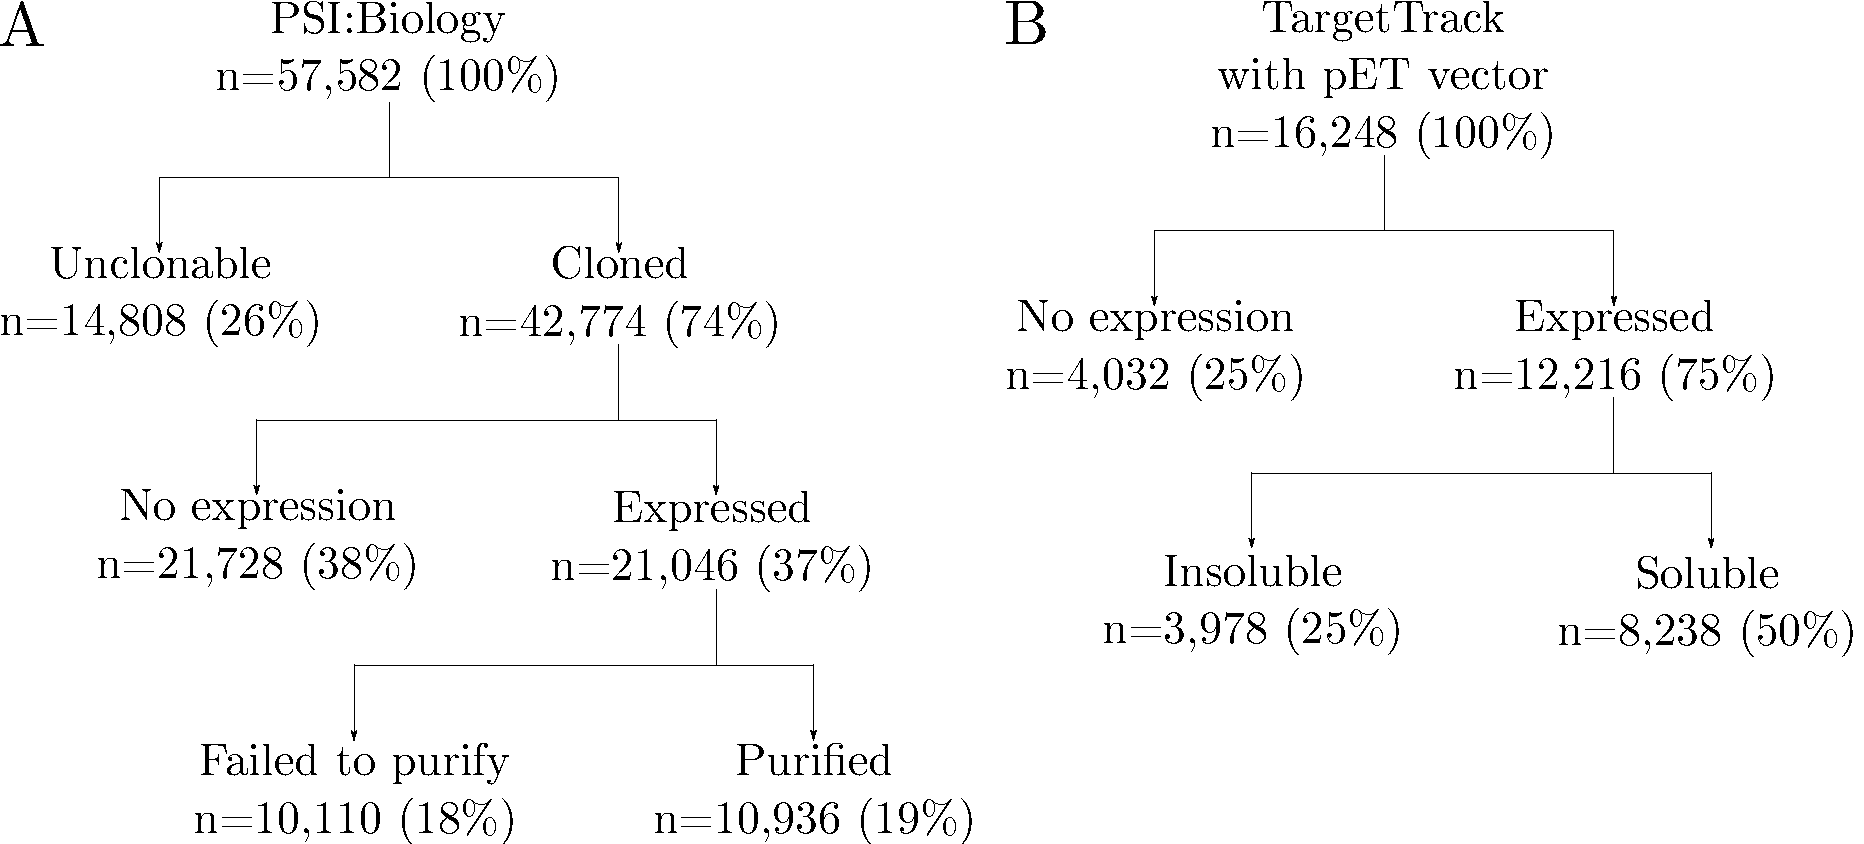
\includegraphics[width=1\textwidth]{chapters/Introduction/Figures/Status_of_protein_expression(2).pdf}
\caption[The success rate of recombinant protein production is around a quarter.]{\textbf{The success rate of recombinant protein production is around a quarter. (A)} All experiments, using different vectors and hosts, preformed for deposition to the TargetTrack database shows around $19\%$ of experiments are purified. Data taken from Protein Structural Initiative (PSI:Biology) metrics. \textbf{(B)} A subset of experiments from TargetTrack database using pET vector and \textit{E. coli} as expression host, shows $50\%$ of experiments produce soluble proteins. }%the List of Figures because of the *}
\label{fig:fail_succ}
\end{figure}


In the following sub-sections, we will discuss these two steps\textemdash protein expression and solubility in details. Unless otherwise stated, these discussions will refer to prokaryotes, in particular, \textit{E. coli} based systems. 

% Protein expression
\subsection{Protein expression}
Protein expression is the process by which protein is synthesised using the information in the messenger RNA (mRNA) (Figure \ref{fig:tranc_transl}). 


\begin{figure}[htbp!]
\center
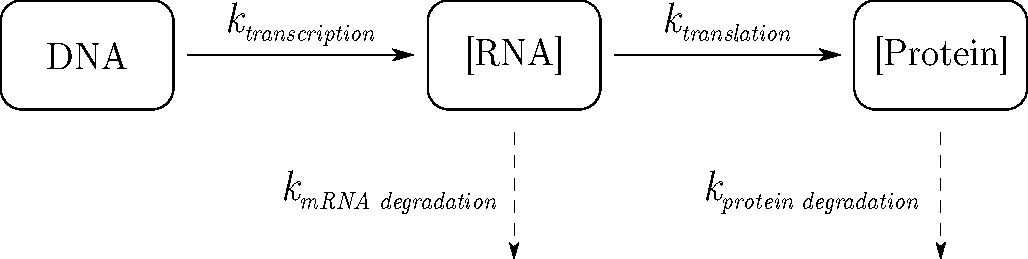
\includegraphics[width=0.7\textwidth]{chapters/Introduction/Figures/transc_transl.pdf}
\caption[Protein expression depends on the rates of RNA and protein synthesis and their degradation.]{\textbf{Protein expression depends on the rates of RNA and protein synthesis and their degradation.} Solid arrow represents synthesis whereas dashed arrow represents degradation. [RNA], concentration of mRNA; [Protein], concentration of protein; $k_{transcription}$, rate of transcription; $k_{translation}$, rate of translation; $k_{mRNA\ degradation}$, rate of mRNA degradation; $k_{protein\ degradation}$, rate of protein degradation. Figure redrawn from Abreu \textit{et al.} (2009).}%the List of Figures because of the *}
\label{fig:tranc_transl}
\end{figure}

Intuitively, we expect the protein yield to be predictable using mRNA levels, the correlation is lower than expected \cite{Abreu2009-zf, Taniguchi2010-uq, Bernstein2002-gg}. This reflects the complexities of the underlying process. The amount of protein produced is determined by translation rate and protein degradation (Figure \ref{fig:tranc_transl}).  This dynamic system can be mathematically described by a first order differential equation \cite{Abreu2009-zf} whose solution at equilibrium gives the following relationship relationship between protein concentration $(P_{\infty})$, mRNA concentration $(R_{\infty})$, translation rate $(k_{translation})$ and protein degradation rate $(k_{protein\ degradation})$ :

\begin{equation}
    \frac{P_{\infty}}{R_\infty} = \frac{k_{translation}}{k_{protein\ degradation}}
\end{equation}

There are various mechanisms regulating translation and protein degradation, so the correlation between $(P_{\infty})$ and $(R_{\infty})$ is not perfect. Squared Pearson's correlation is around $0.4$ for many organisms \cite{Abreu2009-zf}. Assuming the protein degradation rate $(k_{protein\ degradation})$ to be a constant, the ratio of $P/R$ depends upon the translation rate $(k_{translation})$ only. Hence, the amount of protein can be modulated by tuning  $k_{translation}$.

\subsection{Translation}

Translation in prokaryotes is \textit{initiated} when the small ribosome subunit $30S$ binds to the Shine-Dalgarno sequence and moves upto the start codon. The currently accepted model is that the initiator tRNA charged with N-formylmethionine, initiation factor (IF-2) and guanosine triphosphate (GTP) binds with this subunit followed by the release of IF-3 \cite{hames2005biochemistry}. This complex is called the 30S initiation complex. IF-1 and IF-2 are released and the large ribosomal subunit $50S$ now binds followed by the hydrolysis of GTP, to form a $70S$ initiation complex. 

After the formation of initiation complex, the decoding of information in the mRNA begins. This is called \textit{translation elongation}. The $70S$ complex consists of three active sites: peptidyl-tRNA site (P site), aminoacyl-tRNA site (A site) and exit site (E site). Initially, the start codon and the successive codon of mRNA is positioned at P site and A site respectively. The initiator tRNA charged with N-formylmethionine is coupled with start codon at the P site and the corresponding aminoacyl-tRNA is coupled to the next codon at the A site through codon-anticodon pairing (Figure \ref{fig:prokaryotic_translation}). Peptide bond is formed between the amino acid carried by tRNA at P and A site to give a dipeptide. tRNA at P site is translocated to E site, tRNA at A site to P site and the ribosome moves along the mRNA. The deactylated tRNA at E site is released. Since the A site is now empty, it receives the next aminoacyl-tRNA and the process continues adding an amino acid to C terminal of the dipeptide. 


Once the ribosome encounters a stop codon, release factor (RF1 or RF2 and RF3) bind to the ribosome resulting in a tranfer of polypeptide to a water molecule rather than aminoacyl-tRNA. The free polypeptide is released from the ribosome and $70S$ ribosome disassociates into $30S$ and $50S$ subunits. This step is called \textit{translation termination}. 

%%TODO - FIGURE FOR TRANSLATION


\begin{figure}[!hbtp]
    \centering
    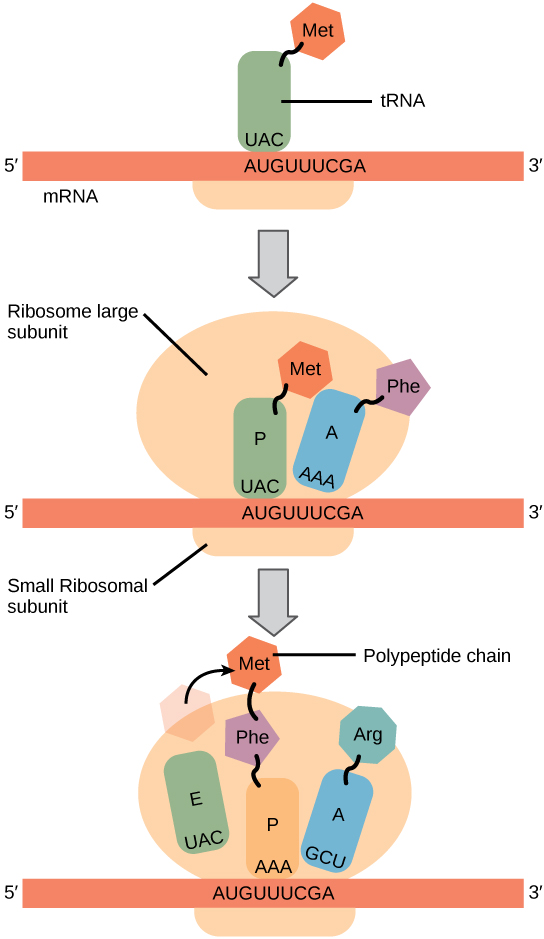
\includegraphics{chapters/Introduction/Figures/translation.jpg}
    \caption[Prokaryotic translation.]{\textbf{Prokaryotic translation.} Initiator tRNA binds to the smaller subunit at the start codon. Larger subunit joins to form a translation initiation complex such that initiator tRNA is at P site and the next aminoacyl-tRNA is at A site. Initiator tRNA moves to the E site, dipeptide is formed at the P site and new aminoacyl-tRNA is received at the A site. Figure from OpenStax College, Concepts of Biology. OpenStax CNX (Creative Commons license: CC BY 4.0) }%the List of Figures because of the *}
    \label{fig:prokaryotic_translation}
\end{figure}


\subsection{mRNA features and their roles in translation}
Translation rate depends on the rate formation of translation initiation complex and utilisation of available tRNA pool. Several features of a mRNA sequence are suggested to explain these two major dependencies of translation rate. However, many mRNA features are not independent, making it hard to distinguish the impacts of individual features \cite{mauger2019mrna}. The features can be classified into three categories: codon preferences, mRNA folding (secondary structure) and mRNA:ncRNA avoidance. These three categories of features is the basis to understand and optimise protein production. Hence, we will describe them in more details:

% mRNA features
%Codon Analysis


\subsubsection{Features based on codon analysis}
This category measures the bias in codon usage relative  to endogenous mRNAs. Higher values of these indices is an indicator that the given mRNA sequence follows the codon usage pattern of the host. Features under this category are the codon adaptation index (CAI) \cite{Sharp1987-ed}, tRNA adaptation index (tAI) \cite{ Reis2004-dl, Sabi2014-je} and related metrics such as codon pair usage \cite{Gutman1989-pn}. For example: the codon adaptation index (CAI) for a given protein is the harmonic mean of the relative adaptiveness $w$ \cite{Sharp1987-ed} of the codons:

\begin{equation}
    CAI_{g}=(\prod_{i=1}^{N} w_i)^{1/N}
    \label{eqn:cai}
\end{equation}
where $w_i$ is the relative adaptiveness of the $i^{th}$ codon which is the ratio of observed frequency of the codon $f_i$ upon consideration to the frequency of the most frequent synonymous codon. $$w_i = \frac{f_i}{max(f_i)}$$ 

Based upon the idea of CAI, tAI was developed to measure the translational efficiency by taking into account of tRNA concentration and codon-anticodon coupling efficiency. We first define the absolute adaptiveness $W_i$ of codon $i$ as:

\begin{equation}
    W_i = \sum_{j=1}^{n_i} (1 - s_{ij})tGCN_{ij}
\end{equation}
where $n_i$ is the number of anticodons pairing with codon $i$, $tGCN_{ij}$ is the copy number of the $j^{th}$ tRNA that recognizes the $i^{th}$ codon. $tGCN_{ij}$ is correlated with the tRNA concentration \cite{kanaya1999studies, novoa2012role}. $s_{ij}$ is a constraint on the codon-anticodon pairing and has values between $0$ (more efficient pairing) and $1$ (less efficient pairing). The relative adaptiveness $w_i$ of the $i^{th}$ codon is  $W_i$ normalised by maximum of $W_i$ among all codons. If $W_i$ is zero, then the relative adaptiveness is the mean of all $W_i$. Once $w_i$ are found, the tAI is the harmonic mean as in Equation \ref{eqn:cai}. 


Both CAI and tAI measures are equivalent to a zeroth order Markov model whereas codon pair usage or di-codon frequency is essentially a first order Markov model. It is thought that a higher value of these indices means that the sequence can utilise the available tRNA pool more efficiently which causes an increase in efficiency of translation \cite{ikemura1985codon, Gutman1989-pn, Sharp1987-ed, Reis2004-dl, Sabi2014-je, Brule2017-mx}. However, this proposition has been challenged and studies suggest that mRNA secondary structure might be more important in explaining translation efficiency.  \cite{Kudla2009-tl, Boel2016-jd, Cambray2018-kn}.

%% Secondary structure
\subsubsection{Secondary structure}
%Translation initiation in prokaryotes begins after the ribosomal $30S$ subunit binds to the Shine-Dalgarno sequence and recognises the start codon. The larger subunit is then assembled to form a translation initiation complex, which moves along the transcript, decoding the codons to form a polypeptide chain. However, if this 
If the region around a translation initiation site forms a strong secondary structure, this leads to disruption of the formation of initiation complex, which inhibits translation (Figure \ref{fig:sec_str_rbs}) \cite{Kudla2009-tl, Espah_Borujeni2014-vy, Tuller2015-ts}. Recent studies show that the RNA structure stability of this region explains variation in protein expression better then codon usage \cite{Kudla2009-tl, Plotkin2011-ak, Cambray2018-kn} indicating that translation initiation is a rate limiting step for translation. Furthermore, secondary structure has been shown to change the functional half-life of mRNA and thus further influence protein expression \cite{mauger2019mrna}. Minimum free energy (MFE) of mRNA is widely used to measure the strength and stability of secondary structure. A way to find the MFE is to enumerate all possible structures of a given mRNA and then find the minimum. However, this is impractical because combinatorial explosion occurs quickly as the length of mRNA increases. Clever dynamic programming algorithms has made this problem tractable the details of which is described below.


\begin{figure}[htbp!]
\center
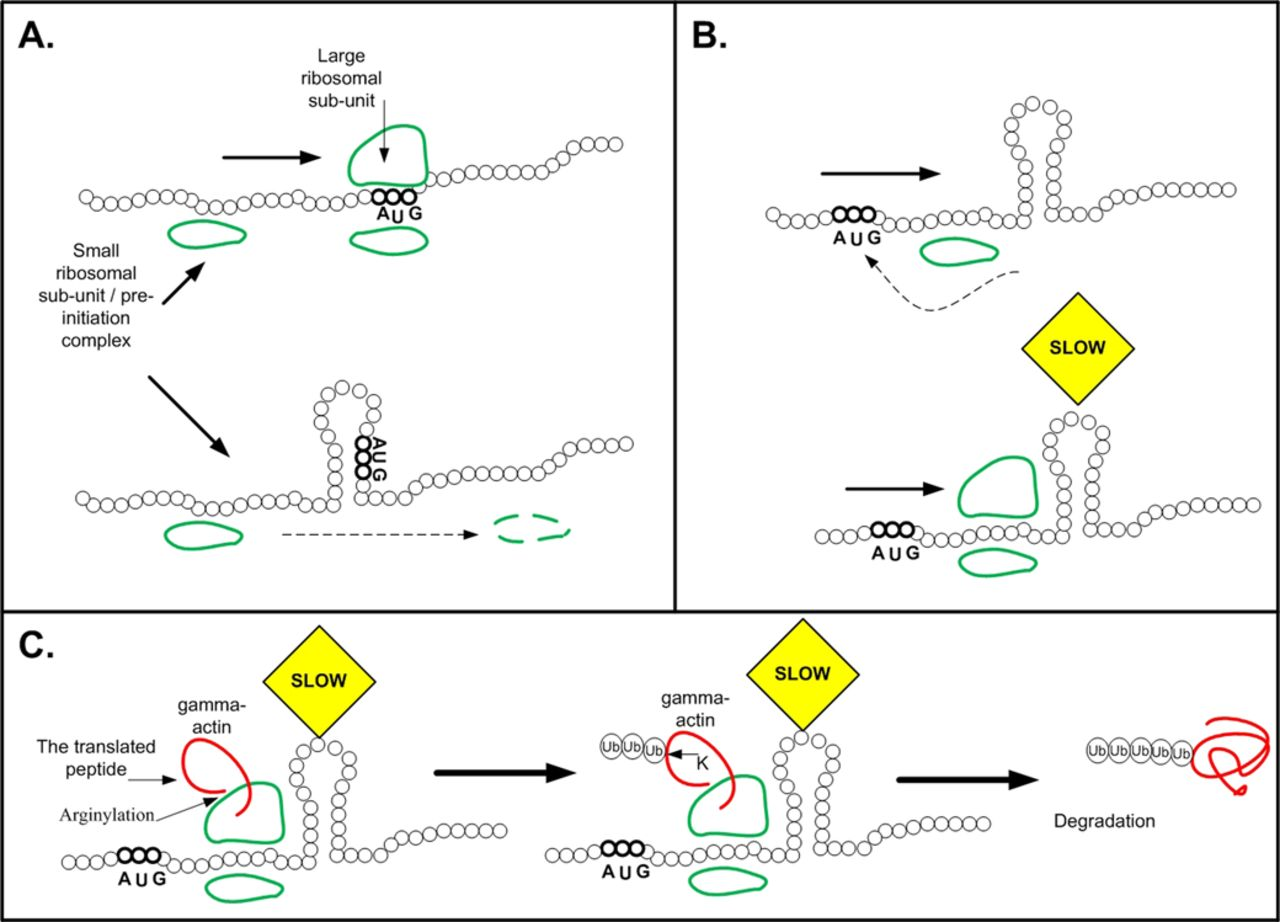
\includegraphics[width=1\textwidth]{chapters/Introduction/Figures/sec_str_rbs.jpg}
\caption[Secondary structure at the translation initiation site inhibits translation.]{\textbf{Secondary structure at the translation initiation site inhibits translation. (A) } The start codon AUG is recognised by the pre-initiation complex if the secondary structure is weak (top) but fails to do so in presence of a strong structure (bottom). \textbf{(B)} Presence of strong structure downstream of translation initiation site prevents the movement of pre-initiation complex (top) which could improve translation efficiency by improving ribosomal allocation (bottom). \textbf{(C)} Such downstream structures could influence post-translation modification by slowing down the ribosome. For example: lysin residues in arginylated gamma actin are exposed due to slow translation and undergo ubiquitination. Figure from Tuller and Zur, (2011) (Creative Commons license: CC BY ) }%the List of Figures because of the *}
\label{fig:sec_str_rbs}
\end{figure}



\paragraph{Computation of minimum free energy (MFE) and suboptimal structures}
Thermodynamically, an RNA structure with the lowest Gibb's free energy is the most stable. This energy is called minimum free energy. Thermodynamic ensembles usually follow the principle of locality, which says that interactions occur only between neighbouring particles. For example: In the Ising model of magnetism, spin interactions happen only between the nearest particles. Similarly, MFE is also calculated by using so called 'Turner parameters' \cite{turner2009nndb} in a nearest neighbouring model and a set of recursive equations called Zuker's algorithm \cite{zuker1981optimal}. However, the accuracy of the computed MFE is only within $5-10\%$ and a large number of alternate RNA structures lie within $5-10\%$ of the predicted global minimum \cite{eddy2004rna}. This prompts us to calculate some other free energies for different suboptimal conformations that RNA may achieve in a near thermodynamic equilibrium. Furthermore, depending on the criteria to pick an \textit{optimal} sturcture from a Boltzmann's ensemble, suboptimal structures may not lie near the thermodynamic equilibrium at all. For example: Ding \textit{et al.} \cite{ding2005rna}  found that structures tend to form clusters in a Boltzmann's ensemble. Instead of free energy, if we use these clusters as a criteria for sampling, then structure that has a minimum distance from all clusters is the optimial structure \cite{lorenz2016predicting}. This structure is also known as centroid structure and other structures around the centroid may as well be regarded as suboptimal.



There were some early attempts to compute suboptimal structures for example, by Zuker \cite{zuker1989finding} and Waterman \textit{et al.} \cite{waterman1985dynamic}. However, the backtracing procedure in their algorithms was not efficient enough to compute energies for longer RNA molecules. This problem was solved by McCaskill \cite{mccaskill1990equilibrium} by proposing an efficient algorithm to compute energy through a partition function which has the same time complexity as Zuker's algorithm for MFE $(\mathcal{O}(n^{3}))$.

\paragraph{Partition function and base pairing probabilities}
Consider a structure $s$ of an RNA molecule with free energy $E(s)$. In a thermodynamic ensemble of different structures at equilibrium, using the principle of maximum entropy, we see that the probability that the given RNA has the structure $s$ follows a Boltzmann distribution:

\begin{equation}
    p(s) \propto e^{-\beta E(s)}
\end{equation}

where $\beta$ is called 'thermodynamic beta' and equals $1/k_B T$, where $k_B$ is the Boltzmann's constant and $T$ is the absolute temperature (Subsection \ref{subsection:sim_anneal} Simulated annealing ). Since sum of probabilities over set of all structures $\Xi$, must be equal to unity, we have:

\begin{equation}
\begin{aligned}
    \sum_s p(s) &= \frac{1}{Z} \sum_{s\in\Xi} e^{-\beta E(s)}  = 1  \\
    Z &= \sum_{s\in\Xi} e^{-\beta E(s)} 
\end{aligned}
\label{eqn:part_func}
\end{equation}

The quantity $Z$, which plays a role of normalisation of probabilities, is called the \textit{canonical partition function}. Many thermodynamic parameters of interest can be derived from $Z$, for example, free energy $G$ of RNA in terms of $Z$ is given by:

\begin{equation}
\label{eqn:free_en}
    G = -\frac{1}{\beta} \ln(Z)
\end{equation}

The efficient dynamic programming to enumerate $Z$ was proposed by McCaskill \cite{mccaskill1990equilibrium} with time complexity of $\mathcal{O}(n^{3})$. This method is essentially a recursive decomposition of $Z$ similar to Zuker's algorithm only difference being the addition in Zuker's relation are now substituted by product because free energies are additive. If $E$ is the total free energy and $E_L$ are the energy contributions from various types of loops (hairpin, stacked pair, bulges, interior loops, multiloops) in a structure, then:

\begin{equation}
    E = \sum_L E_L
    \label{eqn:free_en_add}
\end{equation}

If we suppose the term $Q_{ij}^b$ accounts for all loops $L$ enclosed by $i,j$, we see that additivity of free energy (Equation \ref{eqn:free_en_add}) implies a multiplicative contribution to the partition function (\ref{eqn:part_func}) which gives the following recursive equation :

\begin{equation}
    Q_{ij}^b = \sum_L e^{-\beta E_L} \prod_{i<h<k<j} Q_{hk}^b
    \label{eqn:mcc_restr_part}
\end{equation}

Using this restricted partition function term for loop contributions, the total partition function between $i^{th}$ and $j^{th}$ nucleotides ($Q_{ij}$) can now be written as:

\begin{equation}
    Q_{ij} = Q_{i j-1} + \sum_{i \leq k <j} Q_{i k-1} Q_{kj}^b
    %where, by convention, Q_{i, i} = Q_{i, i-1} = 1.
    \label{eqn:mcc_full}
\end{equation}

The full partition function of RNA with $N$ nucleotides is given by $Z = Q_{1N}$. Equations \ref{eqn:mcc_restr_part} and \ref{eqn:mcc_full} are McCaskill's recursions for partition function. Once $Z$ is known, the probability of any structure $s$ with free energy $E(s)$ is given by:

\begin{equation}
\label{eqn:prob_part_func}
    p(s) = \frac{1}{Z} e^{-\beta E(s)}
\end{equation}

The computational approach outlined above is very generic and can be used for other specific cases. For example: if we want to know the probability that $[i^{th}, j^{th}]$ nucleotides are paired, then we can modify Equation \ref{eqn:part_func}, where partition function is found by simply summing Boltzmann's factor over all structures $\zeta$ where $[i^{th}, j^{th}]$ nucleotides are paired ($\zeta \subseteq \Xi$, where $\Xi$ is the ensemble of structures):

\begin{equation}
    Z_p = \sum_{s\in\zeta} e^{-\beta E(s)}
\end{equation}

The base pairing probabilities are, given by equation \ref{eqn:prob_part_func} with an appropriately computed $Z$. % which is Z on the above equation.


%% Avoidance
\subsubsection{mRNA:ncRNA avoidance}
Recently, Umu et al \cite{Umu2016-zq} found that in bacteria and the archaea, the strength of interactions between mRNAs and non-coding RNAs (ncRNAs) anti-correlate with protein levels. These signals are particularly obvious at the translation initiation site, suggesting that there is an avoidance of inappropriate interactions for highly expressed proteins. However, from a large pool of mRNA and ncRNA, a complete avoidance of interactions is unlikely and a trade off exists between interactions and protein expression. Further, it is suggested that compartmentalisation should minimise these cross talk interactions in eukaryotes. Compartmentalisation has been a topic of considerable research and is linked with noise filtering in gene expression and cellular feedback process \cite{rao2002control, stoeger2016passive, banani2017biomolecular, dong2017shaping}. We now outline in brief, the necessary background to understand the computation of RNA interactions and mRNA:ncRNA avoidance.


\paragraph{Unpairing of bases and accessibility}
McCaskill’s equations \ref{eqn:mcc_restr_part} and \ref{eqn:mcc_full} for the partition function can also be `inverted' to find the probability that $[i^{th}, j^{th}]$ nucleotides are unpaired in the given ensemble. The energy required to unpair the nucleotides is called accessibility or opening energy. If $\kappa \subseteq \Xi$ is the set of all structures $s$ where $[i^{th}, j^{th}]$ nucleotides are unpaired, then the accessibility is given by :

\begin{equation}
\begin{aligned}
    E_{accessibility} &= E_{s \in \kappa} - E_{s \in \Xi}\\
    E_{accessibility} &= -\frac{1}{\beta}\ln{\frac{Z_{unpaired}}{Z}}
\end{aligned}
\end{equation}

The term $\frac{Z_{unpaired}}{Z} = p_u$ is the probability that $[i^{th}, j^{th}]$  nucleotides  are unpaired \cite{Bernhart2011-cc}. Since the pair $i,j$ may or may not be enclosed by a base pair $k,l$ $\ni$ $\forall$ $k,l :$ $ k < i  < j < l$ (Figure \ref{fig:part_fun_decomp}), this probability can be computed by McCaskill approach \cite{Bernhart2011-cc}. Accessibility prediction forms the basis of RNA:RNA interactions. 



\begin{figure}[htbp!]
\center
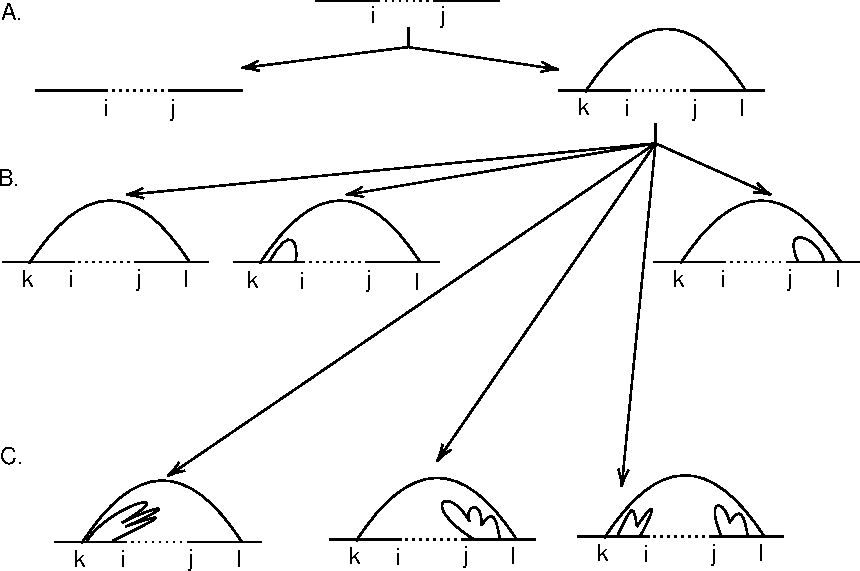
\includegraphics[width=1\textwidth]{chapters/Introduction/Figures/accs.pdf}
\caption[Decomposition of partition function to calculate unpairing probability of the region $(i,j)$ in a nucleotide sequence.]{\textbf{Decomposition of partition function to calculate unpairing probability of the region $[i,j]$ in a nucleotide sequence. (A)}  The interval [i,j] may either be enclosed by pair [k,l] (right) or may be open (left). \textbf{(B)} The enclosed pair may or may not contain an hairpin or \textbf{(C)} multiloops. The partition function $Z_{unpaired}$ is a sum of all these contributions.  Figure adapted from Bernhart \textit{et al.}, (2011)}%the List of Figures because of the *}
\label{fig:part_fun_decomp}
\end{figure}


% The exact equation to compute this probability and the accessibility in $\mathcal{O}(n^{3})$ time is given by Bernhart \textit{et al.}  with an algorithmic implementation in RNAplfold of ViennaRNA suite \cite{Lorenz2011-rg}. Accessibility prediction forms the basis of RNA:RNA interactions. 


\paragraph{RNA:RNA interactions} \label{subsec:rna_interac}
For two RNA molecules to interact and pair, most computational tools assume that this is  a two step process\textemdash unfolding of the RNA molecules at the target sites, followed by an actual interaction (hybridisation) \cite{Muckstein2006-ys}.
Thus, the total binding energy $\Delta G$ is the sum of the accessibility of the target site of the longer RNA molecule $\Delta G_{unpaired}$ and the subsequent interaction between the unfolded region of the interacting molecules $\Delta G_{int}$. $\Delta G_{unpaired}$ is computed by equation $1.8$, where as $\Delta G_{int}$ is computed through equation \ref{eqn:free_en} by replacing $Z$ with $Z_{int}$. For an interaction between nucleotides $[i, j]$ and $[i^*, j*]$ the partition function $Z_{int}$ is given by \cite{Muckstein2006-ys} (Figure \ref{fig:part_fun_interac}):





\begin{equation}
\begin{aligned}
    Z_{int} &= p_u[i,j] \sum_{i^*>j*} Z^I[i,j,i^*,j^*] \\
    where, \\
    Z^I[i,j,i^*,j^*] &= \sum_{\substack{i<k<j\\
    j*<k^*<i^*}} Z^1[i,k,i^*,k^*] e^{E_I(i,k,i^*,k^*)}
\end{aligned}
\end{equation}

with $E_I(i,k,i^*,k^*)$ as the free energy of the interior loop enclosed by $(i,k)$ and $(i^*,k^*)$ and $Z^1[i,k,i^*,k^*]$ contains at least one substructure between $(i,k)$ and $(i^*,k^*)$. 

\begin{wrapfigure}{r}{0.5\textwidth}
  \begin{center}
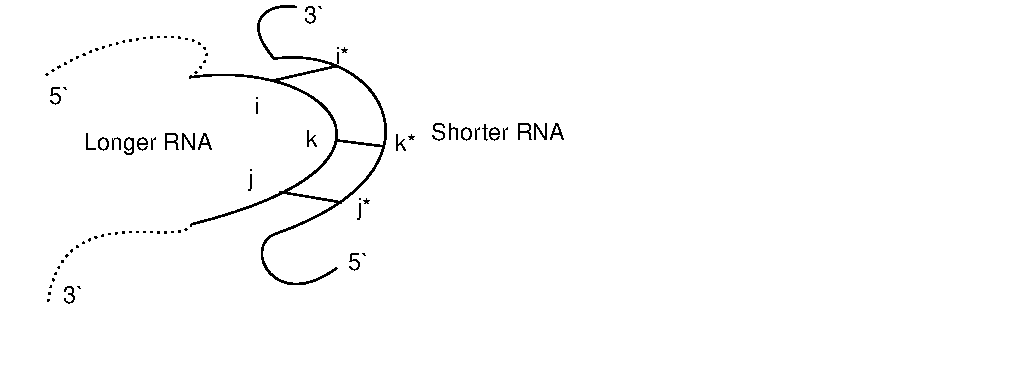
\includegraphics[width=0.7\textwidth]{chapters/Introduction/Figures/interac.pdf}
\caption[RNA:RNA interaction and notations used for partition function.]{\textbf{RNA:RNA interaction and notations used for partition function.} Full shape of longer RNA is not shown. The nucleotides between $[i,j]$ and $[i^*,j^*]$ may contain mismatches. Figure adapted from Muckstein \textit{et al.}, (2006). }%the List of Figures because of the *}
\label{fig:part_fun_interac}
  \end{center}
\end{wrapfigure}

The RNA:RNA interaction prediction mechanisms are still being actively refined because many RNA:RNA interactions have important regulatory functions. For example, in eukaryotes, microRNAs can reduce the levels of mRNAs by interacting with the $3^{\prime}$UTRs of the mRNA targets \cite{catalanotto2016microrna, valencia2006control}.










Apart from these general mRNA features which play a role in protein expression, several specific features also exist. For example: Cis-regulatory elements such as promoters and enhancers, interactions of mRNA with sRNA and miRNA as well as introns in $5^{\prime}$ UTR in eukaryotes. However, our discussion will be based around the general features only. 


A number of gene optimisation tools build a suitable cost or fitness function using a combination of these features. Typically, a genetic algorithm is then used to optimise the fitness. The synonymous mRNA sequence with the maximum fitness is regarded as the optimised mRNA sequence with optimal expression \cite{Villalobos2006-nx, Salis2009-dh, Raab2010-eg, Chung2012-zh, Terai2016-vp}. Despite being optimised on expression, the sequences may form aggregates, which cannot be used for further studies \cite{gustafsson2004codon, rosano2009rare}. This leads us to the discussion of optimising solubility. 


% Solubility
\subsection{Protein solubility}
% The Gibb's phase rule describes the state of a system at equilibrium and is given by 

% \begin{equation}
%     f + p = c + 2
% \end{equation}

% where $c$ is the number of components, $p$ is the number of phases and $f$ is the degree of freedom. For a two phase system (solid and liquid) at constant pressure and temperature, with two components (solute and solvent for example, protein and water), $f = 0$. This means the amount of protein in solution phase no longer depends upon the total amount of protein in the system and remains constant \cite{arakawa19853}. Thermodynamically, the chemical potential of protein in solid phase and liquid phase are now equal. The physical solubility, thus, can be defined as the concentration of protein in a saturated solution which is in equilibrium with the solid phase. Solubility has units of moles per liter ($m/L$) and often, for convenience, written in grams per liter ($g/L$). 


% This physical solubility of a protein depends on the experimental conditions such as temperature, pH, ionic concentration \cite{Kramer2012-wk}. This might lead to the variability of results across various experimental conditions. Hence, 
Solubility is defined as the proportion of the supernatant fraction, obtained after the centrifuging the the translation mixture, to the uncentrifuged total protein \cite{Niwa2009-ye}. It ranges from $0\%$ to $130\%$ with solubility less than $30\%$ categorised as aggregation-prone and greater than $70\%$ are highly soluble. Several \textit{intrinsic} features of the protein itself such as molecular weight, flexibility, hydrophobicity, isoelectric point and structural propensities are also known to influence solubility \cite{Wilkinson1991-zp, Chiti2003-zk, Tartaglia2004-wm, Diaz2010-md}. Sometimes these intrinsic features are modified by doing either mutagenesis or truncation, which might assist in improving solubility. Several solubility enhancing tags are also available for example, thioredoxin (TRX), maltose binding protein (MBP), small ubiquitin-related modifier (SUMO) and glutathione S-transferase (GST). Although, the exact mechanisms of how these tags work is still unclear, it is proposed that they might act like a chaperone and assist in correct folding of the target protein or add charges which decreases the overall aggregation propensity \cite{Costa2014-oe}.

\subsubsection{Intrinsic properties of a protein}
Intrinsic properties are derived from different properties of the residues inside the poly-peptide chain. The commonly used intrinsic properties of proteins are described below.

\paragraph{Hydrophobicity}
Water soluble proteins fold such that the hydrophilic parts are exposed and can form hydrogen bonds with the water molecules whereas the hydrophobic parts are buried in the core. This hydrophobic effect is thought to be responsible for protein solubility \cite{tanford1978hydrophobic}. Several scales have been proposed to measure the hydrophobicity of residues \cite{Kyte1982-qn, abraham1987extension, janin1979surface, rose1985hydrophobicity}. However, none of these scales can fully model the full range of behaviour of residues \cite{charton1982structural}. 


We will use Kyte-Doolittle's scale \cite{Kyte1982-qn} for representative purposes. In this scale, residues are given a hydropathy score such that positive scores represent hydrophobicity and negative score represent hydrophilicity. The magnitude of score represents the strength. For example: isoleucine (I) is given 4.5 and is the most hydrophobic residue, where as  arginine (R) is given -4.5 and is the most hydrophilic residue. Using these scores, a hydropathy plot for a given polypeptide can be drawn (Fig. \ref{fig:hydrophobicity_flexibility_plot}). Hydropathy plot can be used to examine the hydrophobicity of protein region of interest. Using hydrophobic effect, we can then infer whether the residue is buried or located on the surface. Furthermore, the overall hydrophobicity of the protein can be determined by averaging the hydropathy scores across the polypeptide chain to obtain the GRand AVerages of hydropathY (GRAVY) score.


\begin{figure}[htbp!]
\center
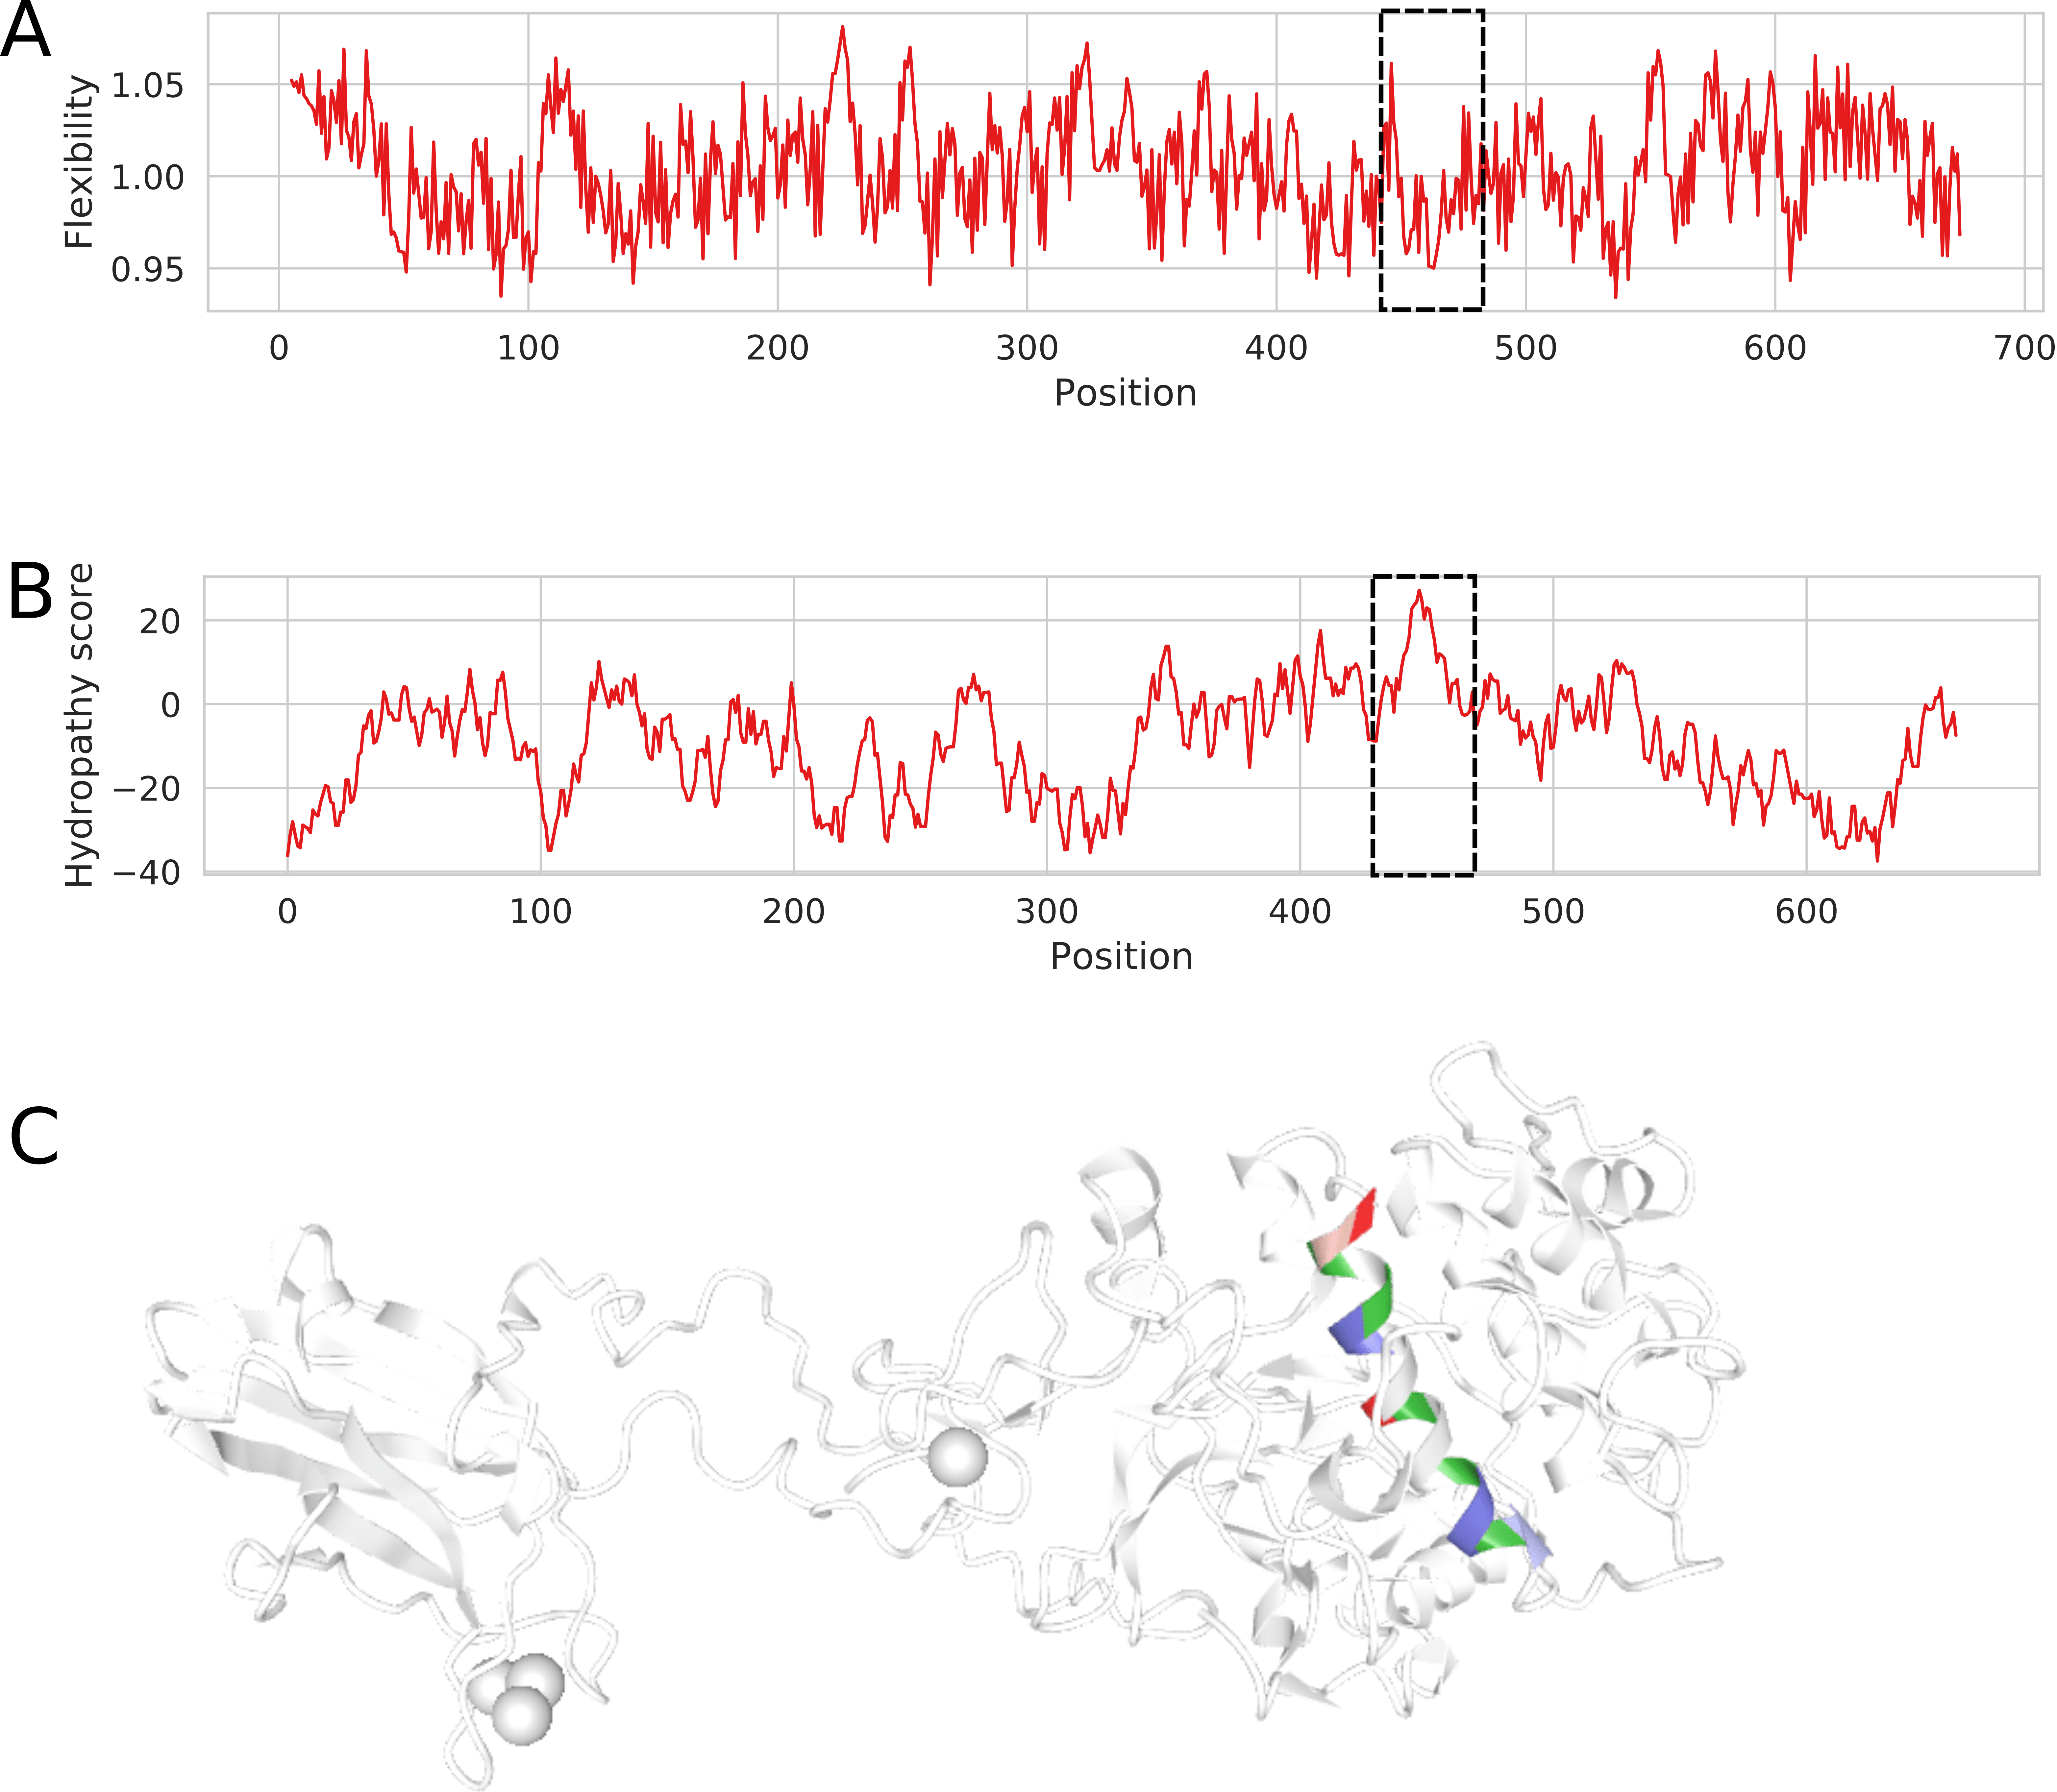
\includegraphics[width=1\textwidth]{chapters/Introduction/Figures/flex_and_hydrop.png}
\caption[Profiles of KPC1\_DROME (UniProtKB P05130).]{\textbf{Profiles of KPC1\_DROME (UniProtKB P05130)}. 
\textbf{(A)} Flexibility plot generated using normalised B-factors from Vihinen et al. (1994), with a sliding window of 9 residues. For these normalised B-factors, values greater than one are regarded to be flexible and values less than one are rigid. \textbf{(B)} Hydropathy plot generated using Kyte-Doolittle's hydrophobicity scale, with a sliding window of 19 residues. For illustration, the hydropathy and flexibility of residues at around position $440$ to $470$ (shown by dotted box) are positive and rigid. This indicates the presence of an alpha helix which is supported by the actual 3D structure \textbf{(C)}. The coloured helix is the region $440$ to $470$.  }%the List of Figures because of the *}
\label{fig:hydrophobicity_flexibility_plot}
\end{figure}


% \begin{figure}[htbp!]
% \center
% 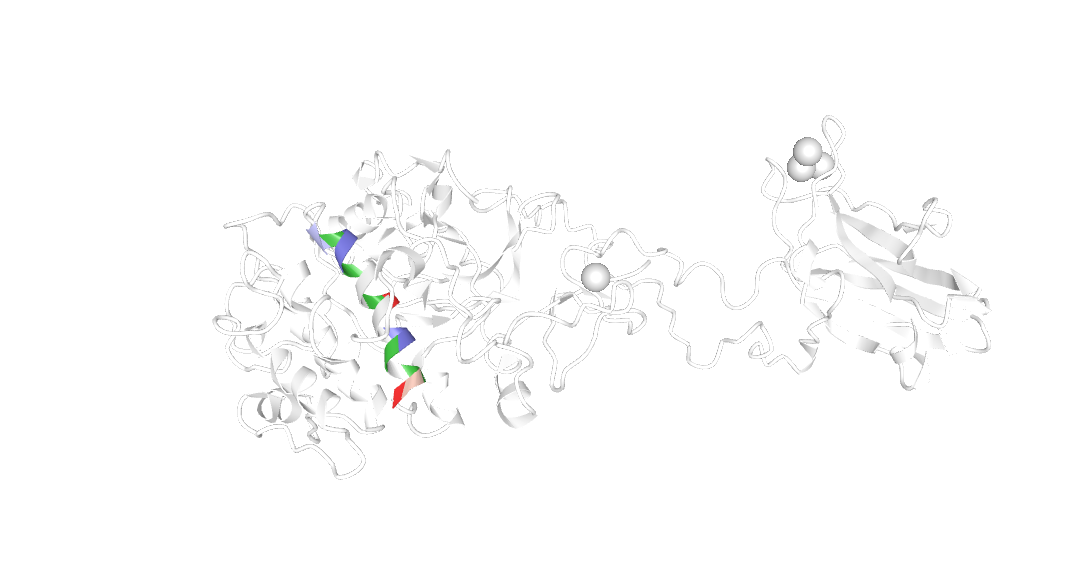
\includegraphics[width=1\textwidth]{chapters/Introduction/Figures/kpc1_drome.png}
% \caption{\textbf{3D structure of KPC1\_DROME (UniProtKB P05130)}. The highlighted helix runs from position $448$ to $467$. The presence of this helix can be inferred by the hydropathy plot (Fig \ref{fig:hydrophobicity_plot}) and the flexibility profile plot (Fig. \ref{fig:flexibility_plot}). }%the List of Figures because of the *}
% \label{fig:3dplot_kpc1_drome}
% \end{figure}


\paragraph{Isoelectric point}
The net charge of a protein at a given pH depends on acid dissociative constant (pKa) of ionisable groups such as amine and carboxyl group. At a certain pH, the amount of negative and positive charge are equal, resulting a zero net charge. This pH is called the isoelectric point (pI). The net charge is positive at pH below pI and negative at pH above pI \cite{shaw2001effect}. Since there are no net charges, the solubility of a protein is minimum at the isoelectric point.

\paragraph{Instability index}
Guruprasad et. al \cite{guruprasad1990correlation} found that the distribution of certain dipeptides on stable and unstable protein is different. Based on 12 unstable and 32 stable proteins, they assigned a weight called dipeptide instability weight value (DIWV) for all dipeptides. The instability index (II) is then given by equation \ref{eqn:instability_index}.

\begin{equation}
    II = \frac{10}{L}\sum_{i=1}^{L-1}DIWV(x_i y_{i+1})
    \label{eqn:instability_index}
\end{equation}

where $L$ is the length of the sequence and $x_i y_{i+1}$ is a dipeptide.

%%%http://pd.chem.ucl.ac.uk/pdnn/refine3/adps.htm
%%Biomolecular Crystallography: Principles, Practice, and Application : page 641

\paragraph{Flexibility}
Protein molecules are dynamic and are inherently flexible due to the motion of the constituent atoms \cite{vihinen1994accuracy, alvarez2014relationship, teilum2009functional}. The structural flexibility of a protein can be inferred by using B-factors \cite{vihinen1994accuracy, Karplus1985-ea, Smith2003-gb}.


The B-factor (Equation \ref{eqn:bfactor}) or temperature factor of the atoms in a crystalline structure is the measure of mean squared displacement vibration around their mean position $(u = \langle (x-x_0)^2 \rangle)$, where $x$ is the displacement of the atom from its mean position $x_0$. B-factor thus reflects the \textit{orderedness} of the crystal lattice and subsequent uncertainty in X-ray scattering structure determination \cite{Schlessinger2005-ps, Carugo2018-ka, Bramer2018-dh}. It has unit of $\AA^2$.


\begin{equation}
    B = 8\pi^2 u
    \label{eqn:bfactor}
\end{equation}

To understand the effect of the B-factor, we define a quantity $f$ called the atomic scattering factor as:

\begin{equation}
    f = \frac{amplitude\ of\ wave\ scattered\ by\ an\ atom}{amplitude\ of\ wave\ scattered\ by\ one\ electron}
\end{equation}

Atomic scattering factor after taking into account of the motion of atom becomes:

\begin{equation}
    f_B = f\cdot e^{-B(sin\ \theta /\lambda)^2}
\end{equation}

where $\theta$ is the Bragg angle and $\lambda$ is the wavelength of the wave. Thus, we see that B-factor attenuates the amplitude of wave scattered by an atom (Figure \ref{fig:bfactors} ).

% \begin{figure}[htbp!]
% \center
% 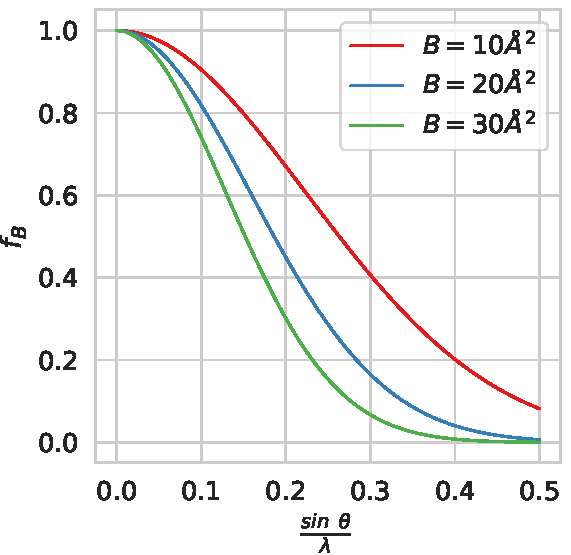
\includegraphics[width=0.5\textwidth]{chapters/Introduction/Figures/bfactors.pdf}
% \caption{\textbf{Attenuation of the incident waves due to increasing B-factor}. As B-factor increases, atomic scattering factor $(f)$ and consequently, the amplitude of wave scattered by an atom decreases rapidly.}%the List of Figures because of the *}
% \label{fig:bfactors}
% \end{figure}

Experimental B-factors for different residues in a protein sequence can be obtained the from Protein Data Bank (PDB). However, due to variation of structures, the B-factor of a given residue varies, even within the same polypeptide chain. For standardisation, the B-factor of residues within a chain are normalised using a z-score.

\begin{equation}
    B_{norm}^i =  \frac{B^i - \langle B\rangle}{\sigma}
\end{equation}

where, $B_{norm}^i$ is the normalised B-factor of residue $i$, $\langle B\rangle$ is the mean and $\sigma$ is the standard deviation of all B-factors across the chain.

\begin{wrapfigure}{r}{0.5\textwidth}
  \begin{center}
    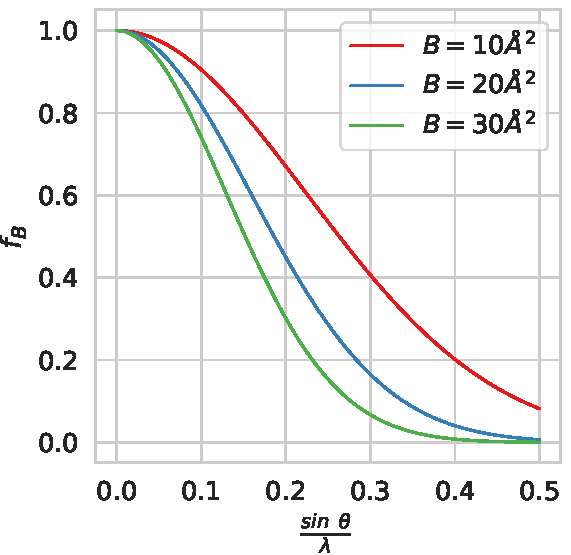
\includegraphics[width=0.45\textwidth]{chapters/Introduction/Figures/bfactors.pdf}
    \caption[Attenuation of the incident waves due to increasing B-factor.]{\textbf{Attenuation of the incident waves due to increasing B-factor.} As B-factor increases, atomic scattering factor $(f)$ and consequently, the amplitude of wave scattered by an atom decreases rapidly.}%the List of Figures because of the *}
    \label{fig:bfactors}
  \end{center}
\end{wrapfigure}


A number of high resolution structures are sampled from database and $B_{norm}^i$ is calculated for each residue on each protein. The mean of $B_{norm}^i$ across the sampled structures is the final normalised B-factor \cite{Schlessinger2005-ps, Smith2003-gb, Karplus1985-ea, vihinen1994accuracy}. 


The structural flexibility of protein can either be determined by using these normalised B-factors from experiments or by directly computing atomic displacements form molecular dynamics simulations (MDS) 
\cite{dong2018structural, kufareva2011methods}. Root mean square fluctuations and radius of gyration from MDS are useful in examining the flexibility. The profile plot (Fig. \ref{fig:hydrophobicity_flexibility_plot}) can be used to visualise and infer the local flexibility and dynamics of the protein structure. Since structural flexibility is inherently related to the protein dynamics, it is thought to influence several properties such as conformal variations, functions, thermal stability, ligand binding and disordered regions  \cite{Vihinen1987-jo, Teague2003-vq, Ma2005-cr, Yuan2005-gl, Yin2011-su, amaral2017protein}. Although the relationship of flexibility with solubility has been noted previously \cite{Tsumoto2003-qp}, it has been overlooked. 


% \begin{figure}[htbp!]
% \center
% 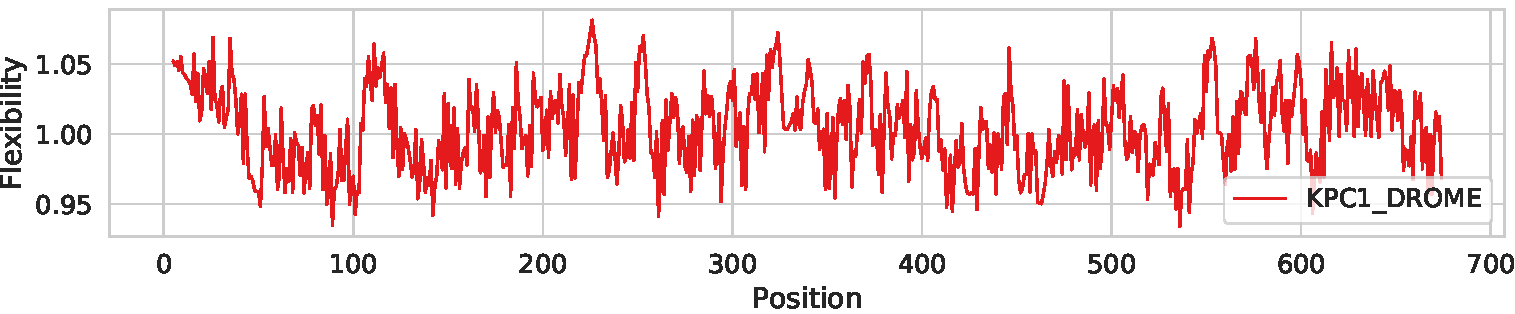
\includegraphics[width=1\textwidth]{chapters/Introduction/Figures/flexibility.pdf}
% \caption{\textbf{Flexibility profile of KPC1\_DROME (UniProtKB P05130)}. Plot was generated using normalised B-factors from Vihinen et al. (1994), with a sliding window of 9 residues. For these normalised B-factors, values greater than one are regarded to be flexible and values less than one are rigid. For illustration purposes, the residues at around position $440$ to $470$ are rigid, suggesting that there might be some structures. This is also supported by the hydropathy plot (Fig. \ref{fig:hydrophobicity_plot}) and the actual 3D structure (Fig. \ref{fig:3dplot_kpc1_drome}).}%the List of Figures because of the *}
% \label{fig:flexibility_plot}
% \end{figure}


Beside these features, amino acids also tend to have different structural propensities which is also thought to influence protein solubility \cite{Idicula-Thomas2005-qw, Huang2012-ft}.


Many solubility prediction tools have been developed around these features using statistical models (e.g., linear and logistic regressions) and machine learning models (e.g., support vector machines and neural networks) \cite{Hirose2013-nq, Habibi2014-jq, Hebditch2017-bg, Sormanni2017-lo, Heckmann2018-wb, Wu2019-nz, Yang2019-kd}. Newer tools such as SOLart also employ 3D structural information for a precise estimation of solvent accessibility, which makes the prediction more accurate \cite{hou2020solart}. Despite a higher prediction accuracy, the usability of these structure based tools might be limited due to the lack of 3D structure information of many proteins of interest.





% Signal peptides
\section{Signal Peptide}
Secretory proteins such as hormones and toxins are some of the commercially important use cases of recombinant protein expression. These secretory proteins are often enriched with a short hydrophobic peptide at the N-terminal (Figure \ref{fig:signal_peptides}). This is called signal peptide (SP). Signal peptides are recognised by a protein complex called the signal recognition particle (SRP). SRP carries the signal peptide to the endoplasmic reticulum (ER) lumen, where post translation modification happens and the newly synthesised protein is secreted out.  Despite having no consensus, SP have a tripartite structure as N-region, H-region and C-region \cite{Von_Heijne1985-qv} (Figure \ref{fig:signal_peptide_structure}). 

\begin{figure}[htbp!]
\center
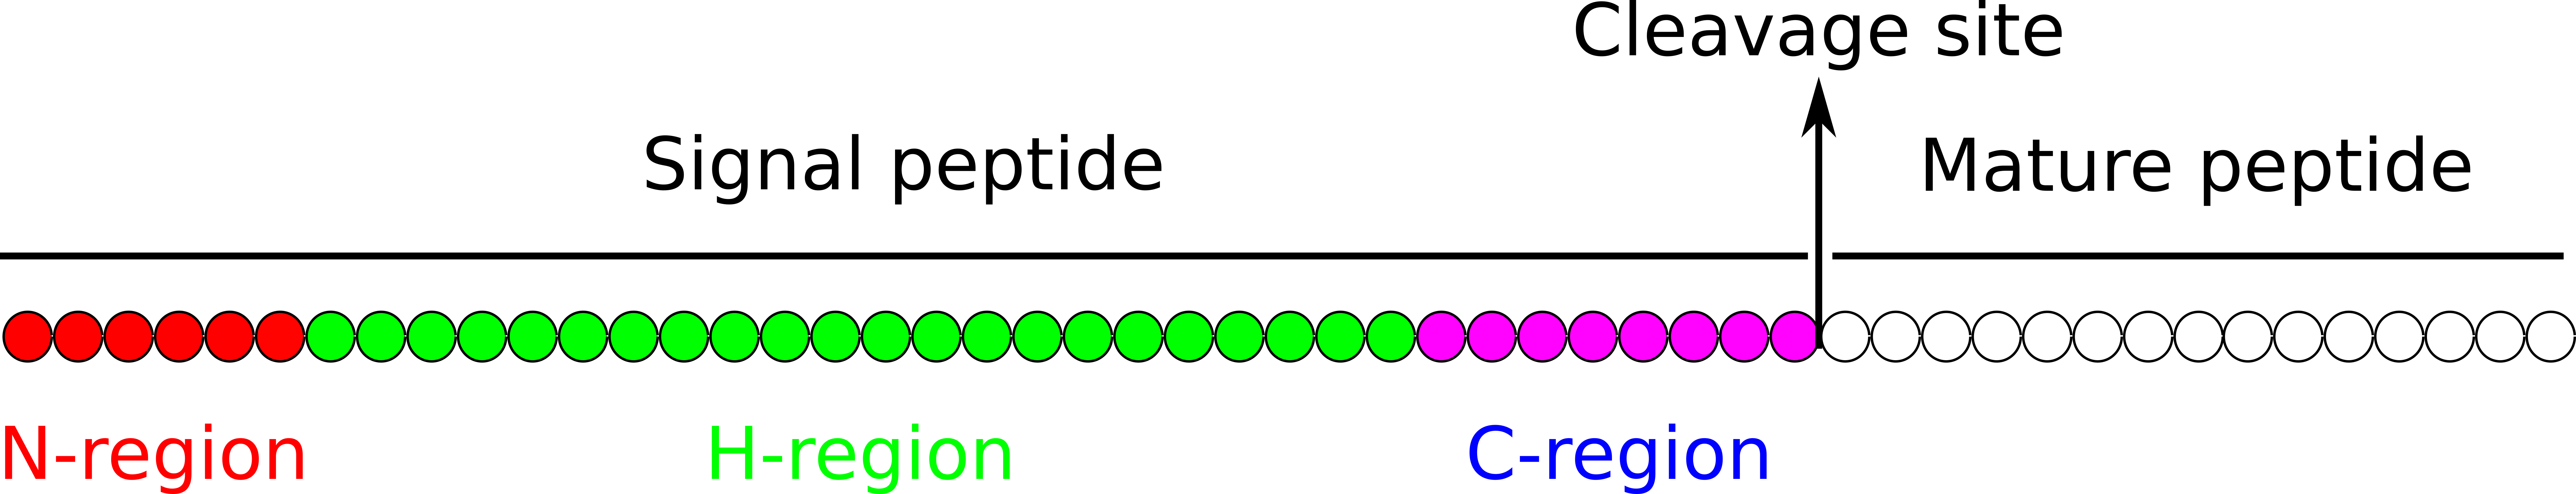
\includegraphics[width=1\textwidth]{chapters/Introduction/SignalPeptide/Figures/signal_peptide.png}
\caption[Tripartite structure of a signal peptide.]{\textbf{Tripartite structure of a signal peptide.} N, H and C domains in a signal peptide. C domain also contains a cleavage site from which mature peptide is cleaved off after reaching the endoplasmic lumen. Sequence logo (bottom) shows an enrichment of Leucine (L) at the H-region.}
\label{fig:signal_peptide_structure}
\end{figure}


\begin{wrapfigure}{r}{0.5\textwidth}
  \begin{center}
    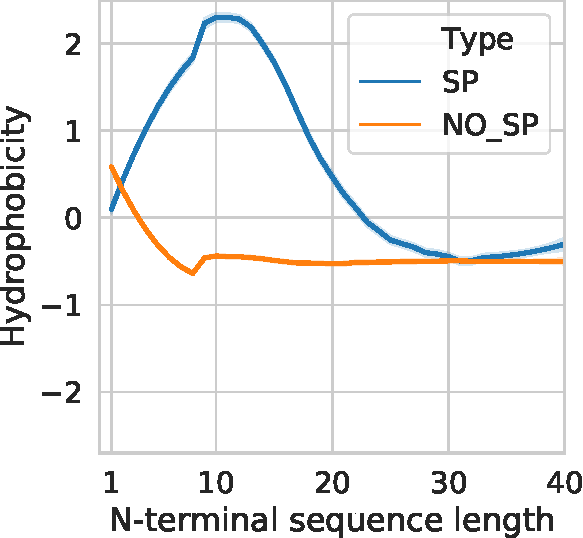
\includegraphics[width=0.45\textwidth]{chapters/Introduction/SignalPeptide/Figures/sp_nosp_lineplot.pdf}
    \caption[Signal peptides are highly hydrophobic at the N-terminal.]{\textbf{Signal peptides are highly hydrophobic at the N-terminal.} Savitzky–Golay filtering is applied to the hydrophobicity. SP (N=2,609) and NO\_SP (N=14,655) sequences from SignalP 5.0 dataset (Armenteros \textit{et al.} (2019)). SP, Signal Peptide; NO\_SP, Not a SP.}%the List of Figures because of the *}
    \label{fig:signal_peptides}
  \end{center}
\end{wrapfigure}
The N-region usually consists of 2-5 charged residues, whereas the H-region is highly hydrophobic and forms an alpha helix. The C-region consists of small polar uncharged residues which often form a $\beta$-sheet structure. This topology is thought to help binding with signal peptidase and cleave off the signal peptide at the cleavage site. 

% Translation is temporarily paused when signal recognition particle (SRP) binds to the SP. SRP then carries the ribosome/mRNA complex towards the translocon of endoplasmic recticulum (ER). Signal peptide is then detached from the mature peptide and possibly digested by signal peptidase. Translation resumes, pushing the nascent polypetide inside the ER lumen, where post translation modification happens and the newly synthesised protein is secreted out. 

The use of signal peptides in recombinant expression can lead to a high yield. As an added benefit, the proteins are often closer to the native activity because proper folding can happen inside the ER \cite{Futatsumori-Sugai2010-iu, Karyolaimos2019-ip}. 



% Optimisation methods
\section{Mathematical optimisation}
Optimisation is a way to find out the best solution to the problem. The starting point for optimisation is to define an objective function or the cost function. For an objective function $f: A \rightarrow  \mathbb{R}$, the goal of optimisation is to find $x_0 \in A$ such that $f(x_0) \leq f(x)$ $\forall\ x \in A$. If the objective function is differentiable, then we can use the gradient information to reach the optimal point. Non differentiable functions are usually optimised by heuristic optimisation methods. Heuristic methods often provide a near optimal solution even if the search space is large. The following optimisation methods are used in this study.


\subsection{Simulated annealing}
\label{subsection:sim_anneal}
Simulated annealing is a heuristic optimisation technique inspired by the way metals cool and anneal. More precisely, it is based on the thermodynamics of a system undergoing a slow cooling so that the atoms have sufficient time to redistribute to form a crystalline structure\textemdash a state of minimum energy  \cite{Kirkpatrick1983-hh, Ingber2000-aw, Keith2002-jx, Brownlee2011-bk, presse1988numerical}. Simulated annealing algorithm is often used to solve combinatorial optimisation problems in bioinfomatics and other sciences. It has been used to align and predict non-coding RNAs from multiple sequences \cite{Lindgreen2007-jy}, to find consensus sequences \cite{Keith2002-jx} and optimise the ribosome binding sites \cite{Salis2009-dh} and mRNA folding using minimum free energy models \cite{Gaspar2013-bg}.

Let $p_i$ is the probability that a system is in certain state $i$ with energy $\epsilon_i$. Then entropy of the system is defined as:
\begin{equation}
    S = -k_B\sum_{i} p_i \ln(p_i)
    \label{eqn:entropy}
\end{equation}
where $k_B$ is the Boltzmann's constant. For any system, the second law of thermodynamics states that the entropy is maximised as the system evolves towards a  thermodynamic equilibrium. Hence, to know the behaviour of the system, Equation \ref{eqn:entropy} needs to be maximised under these two constrains:
\begin{equation}
    \begin{split}
        1)\ \sum_j p_j &= 1 \\
        2)\ \sum_j p_j \epsilon_j &= E
    \end{split}
\end{equation}
The first condition simply means that sum of all probabilities should be unity while the second condition implies the total energy of the system is constant. Using Lagrange multipliers,  
\begin{equation}
    S = -k_B\sum_j p_j \ln(p_j) - \lambda [\sum_j p_j -1 ] - \beta[\sum_j p_j \epsilon_j - E]
    \label{eqn:lagrange_mult}
\end{equation}
Setting the first derivative of Equation \ref{eqn:lagrange_mult} to zero, we obtain:
\begin{equation}
    p_i = e^{1-\lambda}.e^{-\beta \epsilon_i}
    \label{eqn:prob_aft_max}
\end{equation}
$\beta$, also known as thermodynamic beta, can be shown to be equal to $1/k_B T$, where $T$ is the absolute temperature. $\lambda$ is chosen to normalise the probability $p_i$ in Equation \ref{eqn:prob_aft_max}. We thus arrive at the Boltzmann's probability distribution:
\begin{equation}
    p_i = \frac{1}{Z} e^{-\beta \epsilon_i}
    \label{eqn:prob_boltzmann}
\end{equation}
where $Z$ is the partition function. For a system in thermal equilibrium at temperature $T$, Equation \ref{eqn:prob_boltzmann} gives us a set of probability mass functions for all different energy states $\epsilon_i$. An interesting implication of the Boltzmann's distribution is that even at low temperature, there is a non zero probability of system being at high energy.  


Mathematical way to reach the minima of the Boltzmann's distribution is by using a Markov chain sampling while simultaneously decreasing the temperature. The decreasing temperature is simulated by applying a cooling schedule, which could be exponentially decreasing \cite{Kirkpatrick1983-hh}. Markov chain sampling can be done by using Metropolis-Hastings algorithm or perhaps Gibb's sampling, although it is less commonly used  \cite{Keith2002-jx}. In Metropolis-Hastings algorithm, a \textit{bad} move (uphill) $E_2$ from initial state $E_1$ such that $E_2 > E_1$, is accepted if $R(0,1) \geq p_2/p_1$, where $R(0,1)$ is a uniformly random number between $0$ and $1$ \cite{hastings1970monte}. Unlike gradient descent, where only \textit{good} moves (downhill) ($E_2 < E_1)$ are accepted, this algorithm thus, can move both uphill and downhill without getting trapped in local minima. The probability of system moving uphill, however, decreases with decrease in temperature \cite{presse1988numerical}. 


%‘bad’ move
A use case of simulated annealing on a Rastrigin function (Figure \ref{fig:rastrigin}) is shown in Figure \ref{fig:sim_anneal}. 

\begin{figure}[H]
\center
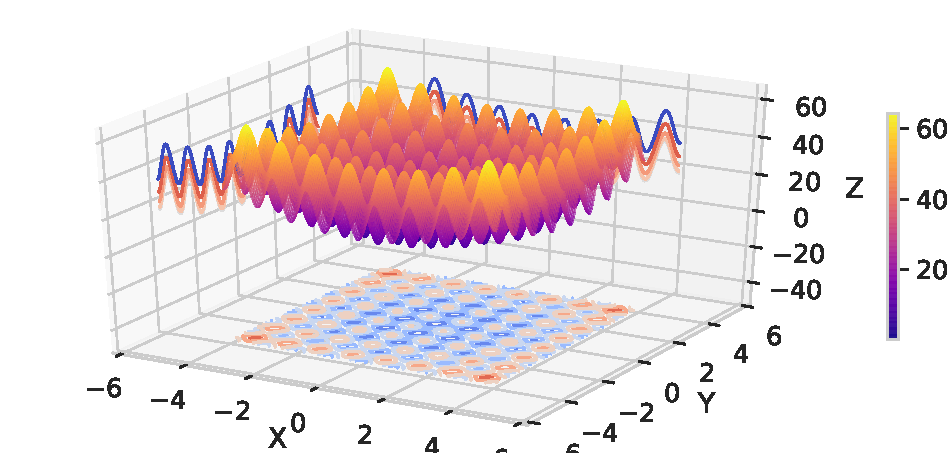
\includegraphics[width=1\textwidth]{chapters/Introduction/Figures/rastrigin.pdf}
\caption[Two dimensional Rastrigin function.]{\textbf{Two dimensional Rastrigin function.} Rastrigin function is frequently used as a test function in optimisation problems because of a large number of local minima. The global minima is at $(0, 0)$ where the value of function is $0$.}%the List of Figures because of the *}
\label{fig:rastrigin}
\end{figure}


\begin{figure}[H]
\center
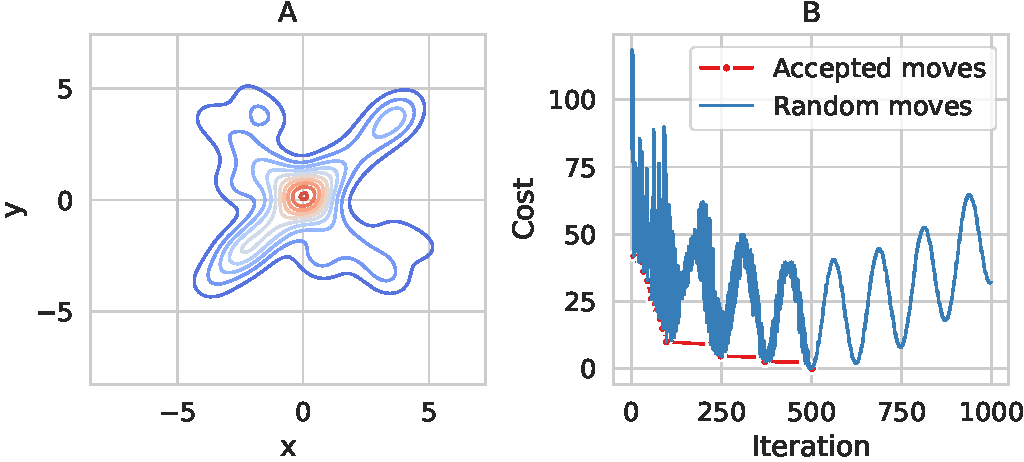
\includegraphics[width=1\textwidth]{chapters/Introduction/Figures/simulated_annealing.pdf}
\caption[Simulated annealing on a two dimensional Rastrigin function.]{\textbf{Simulated annealing on a two dimensional Rastrigin function.} This simulation was run for $1,000$ iterations with an initial temperature of $1$. The minimum found was at $(0.006, -0.013)$, where the value of function was $0.04$.  \textbf{(A)} Kernel density estimate of the moves during simulated annealing shows that they converge near the true minimum $(0, 0)$. \textbf{(B)} The accepted costs are usually immune to the traps of local minima. The algorithm converted at $502^{nd}$ iteration, where the accepted cost is $0.04$. This is close to the global minima $0$. }%the List of Figures because of the *}
\label{fig:sim_anneal}
\end{figure}


\subsection{Nelder-Mead method}
The Nelder-Mead method is another type of derivative-free, heuristic optimisation technique \cite{Nelder1965-zb}. The method, however, requires the objective function to be evaluated at different points hence can also be categorised as a \textit{direct search} method. Direct search methods usually employ a non-degenerate simplex at each step \cite{lagarias1998convergence}. 

% \footnote{Simplex in $n$ dimensions is a convex-hull of $n+1$ vertices and can be understood as a generalisation of triangles. By non-degenerate, we mean the volume of the simplex is non zero.}

For an $n$ dimensional function $f(x)$, initialisation is done by choosing $n+1$ points $(x_i, 1\leq i \leq n+1)$ which form a simplex. These points are ordered such that $f(x_1) \leq f(x_2) \leq ... f(x_{n+1})$. Since the goal is to minimise $f(x)$, in this case $x_{n+1}$ is the worst point and $x_1$ is the best. The worst point is then reflected along the centroid of the simplex to give a new vertex $x_r$ such that the volume is preserved and the non-degeneracy is maintained \cite{presse1988numerical}. Three cases may happen:

\begin{itemize}
  \item $f(x) \leq f(x_r) \leq f(x_{n+1})$
  
  In this case, the new move is neither good nor bad. $x_r$ replaces some older point $x_o$ where $f(x) \leq f(x_o) \leq f(x_{n+1})$.
  
  \item $f(x) \leq f(x_{n+1}) \leq f(x_r) $
  
  In this case, the new move is worst. The simplex is contracted by decreasing $x_{n+1}$ to $x_c$. If $x_c < Min(f(x_{n+1}), f(x_r))$, $x_{n+1}$ is replaced by $x_c$. Else, contraction is repeated.
  
  \item $f(x_r) \leq f(x_1) \leq f(x_{n+1}) $
  
  In this case, the new move is good. $x_r$ replaces the older best point $x_1$. 
\end{itemize}

The ordering of points and reflection are repeated, until the change in the value of the function at the best point falls below a preset tolerance. This method tends to get stuck at local minima (Figure \ref{fig:nelder-mead} A, B), because whenever it encounters one, the algorithm contracts the simplex rather than exploring the surrounding. However for functions with a few or no local minima, for example, Rosenbrock function (Fig. \ref{fig:rosen}), if the starting point is good, this algorithm is very efficient in finding the minima (which is often global) (Figure \ref{fig:nelder-mead} C, D).


\begin{figure}[H]
\center
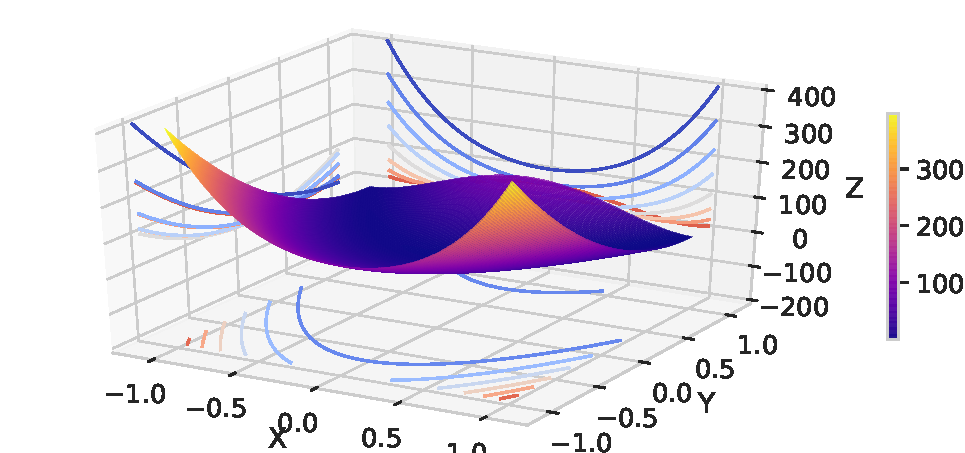
\includegraphics[width=0.75\textwidth]{chapters/Introduction/Figures/rosen.pdf}
\caption[Two dimensional Rosenbrock function.]{\textbf{Two dimensional Rosenbrock function.} Rosebrock function has a characteristic valley where the global minimum lies. The global minima is at $(1, 1)$ where the value of function is $0$.}%the List of Figures because of the *}
\label{fig:rosen}
\end{figure}

\begin{figure}[H]
\center
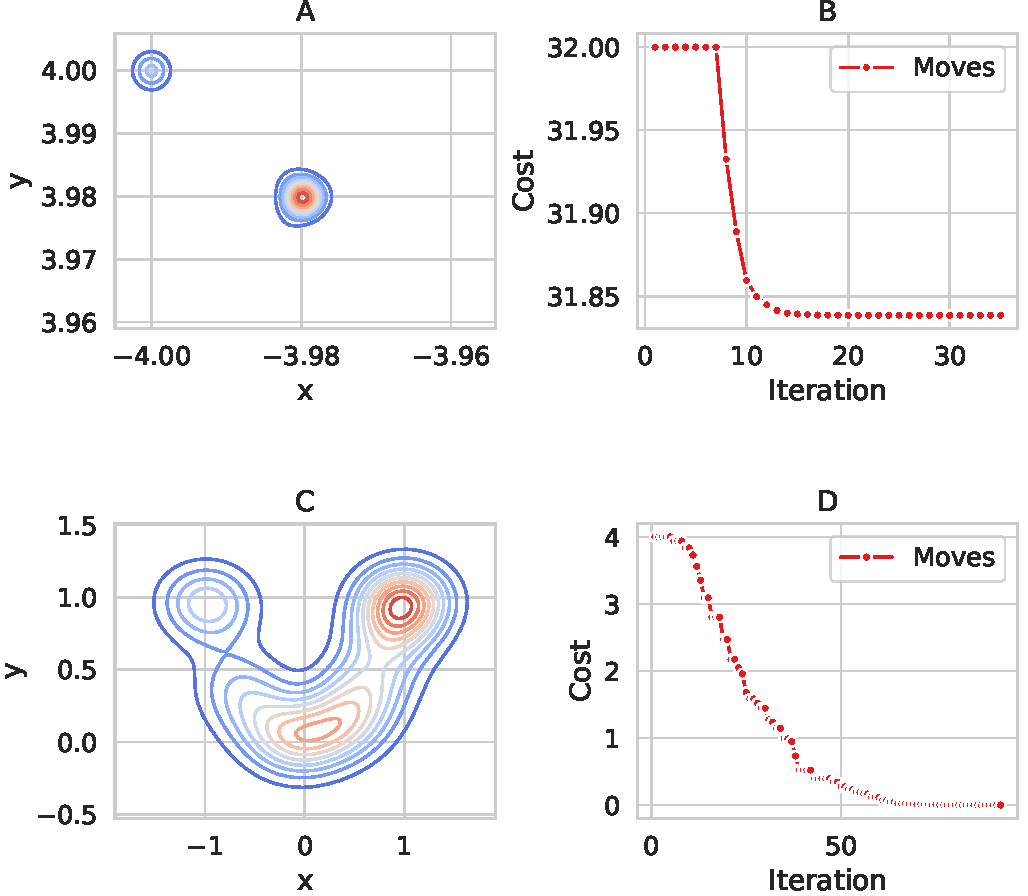
\includegraphics[width=0.75\textwidth]{chapters/Introduction/Figures/Nelder-Mead.pdf}
\caption[Although the Nelder-Mead method tends to get stuck on local minima, a good initial point can result in a global optimum.]{\textbf{Although the Nelder-Mead method tends to get stuck on local minima, a good initial point can result in a global optimum.} \textbf{(A)} Nelder-Mead method applied on a Rastrigin function. Kernel density estimate of the moves shows that the algorithm gets stuck at a local minima $(-3.98, 3.98)$. \textbf{(B)} The algorithm terminated after $35$ iterations where the minimum was found to be $3.36$, which is a local minimum. \textbf{(C)} Nelder-Mead method applied on a Rosenbrock function with $(-2,2)$ as the starting point. Kernel density estimate of the moves shows that the algorithm moves around the valley and terminates at $(1.0001, 1.0002)$ close to the global minima. \textbf{(D)} The algorithm terminated after $92$ iterations where the minimum was found to be $3.36 \times 10^{-8}$.}%the List of Figures because of the *}
\label{fig:nelder-mead}
\end{figure}

% Classifier
\section{Classifiers}
Classifiers are functions which map the input vector to some specific category. In the context of machine learning, we usually use a set of labelled data (known as training data) to fit a classifier. This fitted classifier, also known as model, can then be used to do predictions on unknown data. Many types of classifiers exist such as linear classifiers, support vector machines, decision trees and neural networks (Figure \ref{fig:classifier_comparision}). One special classifier built from an ensemble of decision trees called the Random forest classifier is used in this work. 

\subsection{Random forest}
A random forest is a classifier consisting of a collection of tree structured classifiers $\{h(x, \Theta_k), k=1, ...\}$ where the  $\{\Theta_k\}$ are independent, identically distributed random vectors and each tree casts a unit vote for the most popular class at input {x} \cite{breiman2001random}. For a given data, a number of decision trees $B$ are constructed using bootstrapping. Every time a new split is done, a subset $m$ of total vectors (features) $f$ is used, such that $m < f$. If $m = f$, this procedure is called bagging. In practise, usually, $m \approx \sqrt{f}$. Surprisingly, the number of trees, $B$, is not critical and setting this to a very high value will not lead to overfitting, which can be shown to be a consequence of strong law of large numbers \cite{james2013introductiontostatlearning, breiman2001random}. This also makes random forests more robust to noise and outliers than other classifiers. 

Typically, each bagged tree uses around two-third of training points. Out-of-bag (OOB) estimates can be computed by preforming predictions on the remaining one-third points. OOB errors reflect the generalisability of the model. For each feature, we can also compute the total reduction of Gini index by that feature at each tree split, where Gini index is defined by: 
\begin{equation*}
    G = \sum_{k=1}^{K}(p_{mk}(1-p_{mk}))
\end{equation*}
and is a measure of variance across $K$ classes for the proportion of training observations, $p_{mk}$, in the $m^{th}$ region that are from the $k^{th}$ class. This gives us the feature importance, sometimes called the Gini importance. However, it should be noted that $m$ features used for each split are actually random and is not based on feature importance at all. This seemingly deceptive strategy forces all the subsequent trees to not use the same strongest predictor, thus forcing a decorrelation among the trees. This makes the outputs less variable and more reliable.

\begin{figure}[!hbtp]
\centerline{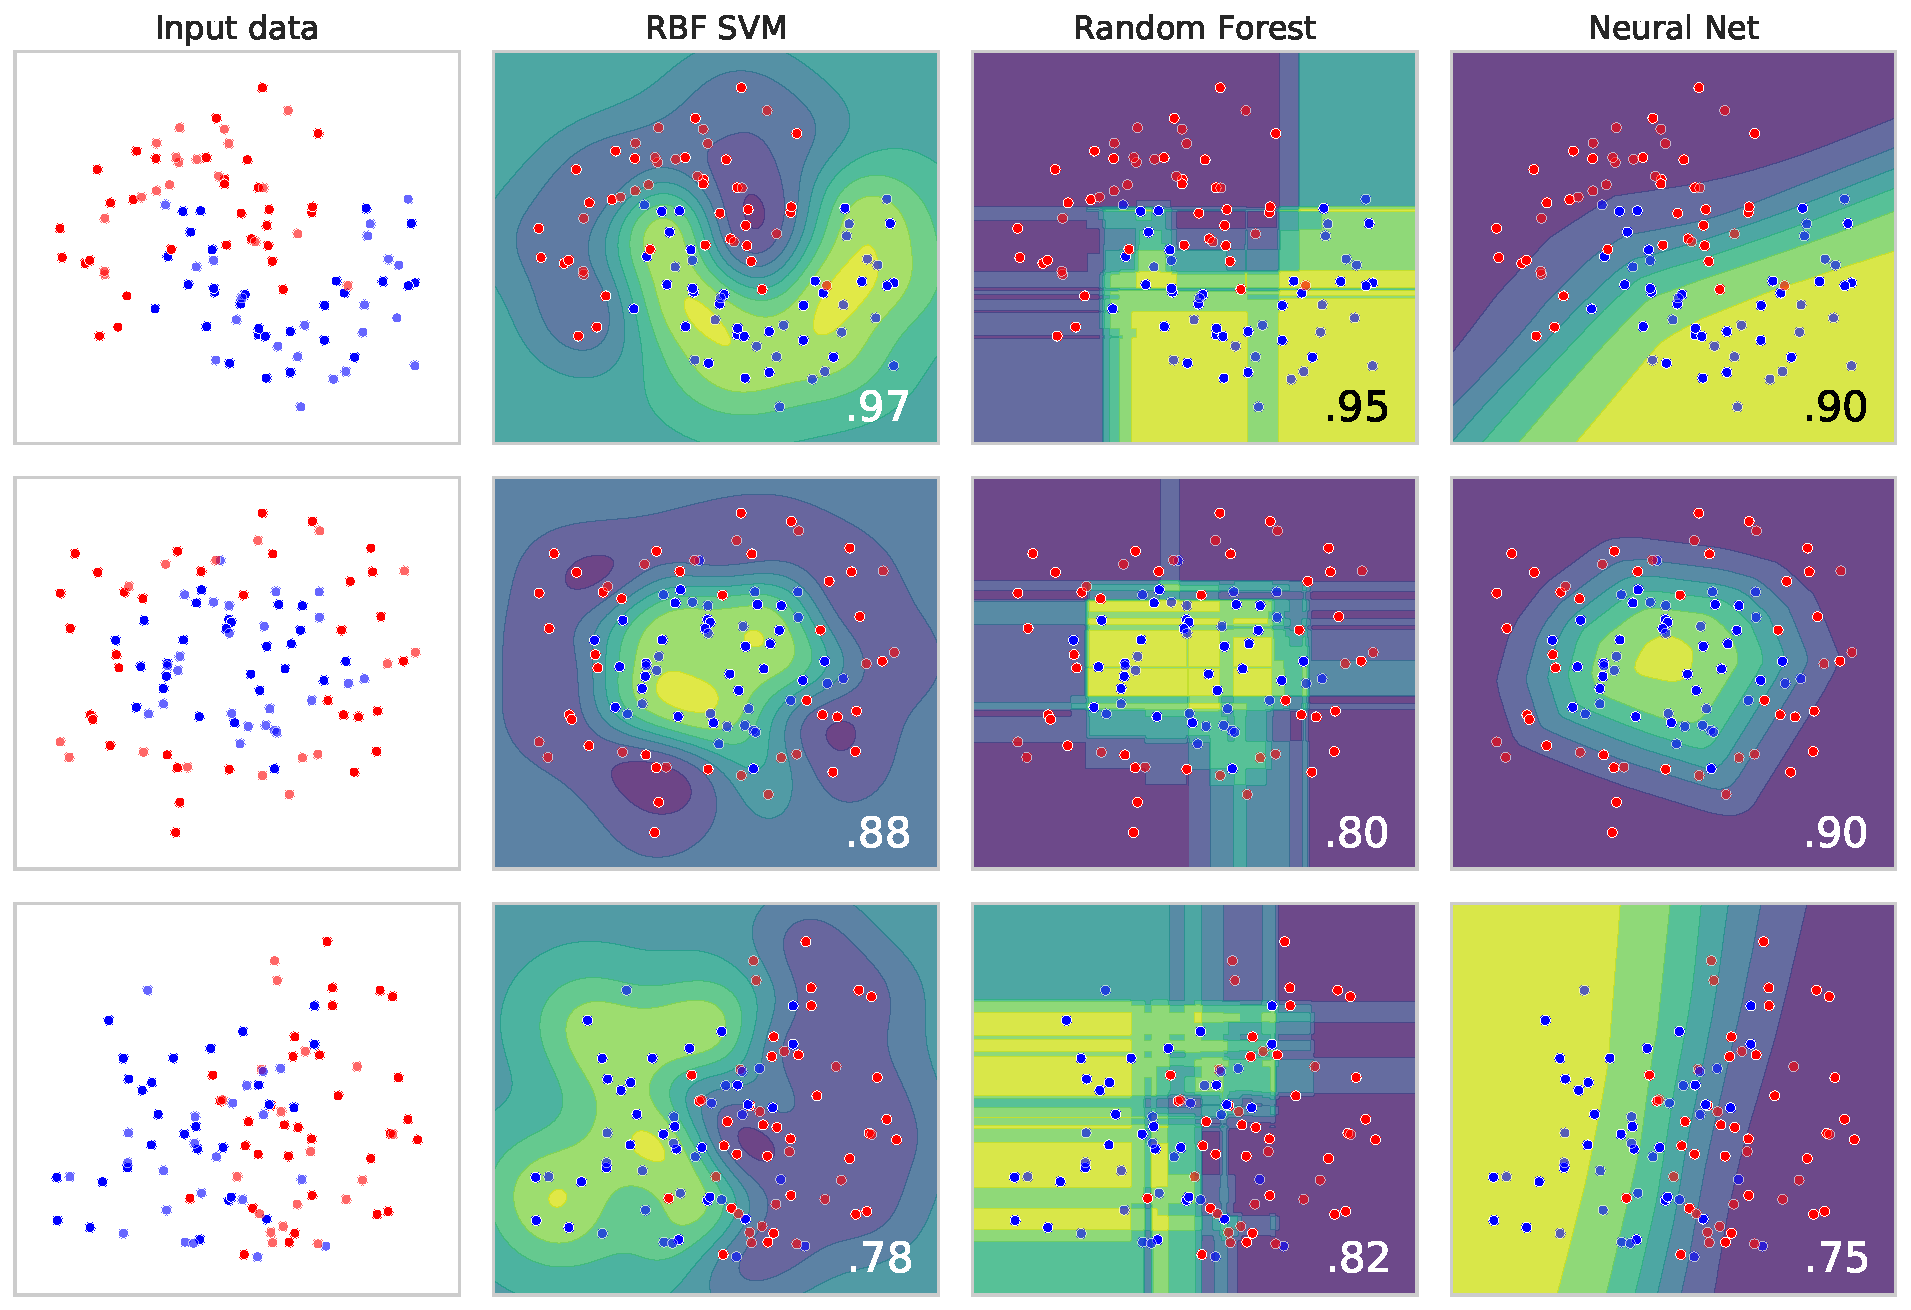
\includegraphics[width=1\textwidth]{chapters/Introduction/Figures/classifier_comparision.pdf}}
\caption[Comparison between some of the commonly used classifiers.]{{\bf Comparison between the some of the commonly used classifiers.} Three commonly used classifiers\textemdash SVM with RBF kernel, Random forest and a simple neural network (multi-layered perceptron) on three synthetic datasets as input. The input data is a binary data coloured as red and blue. The decision boundary is shown as contours and the accuracy of each classifier is shown on bottom right. Adapted from https://scikit-learn.org/stable/auto\_examples/classification/plot\_classifier\_comparison.html. SVM, Support Vector Machine; RBF, Radial Basis Function.}\label{fig:classifier_comparision}
\end{figure}








\chapter{Protein yield is tunable by synonymous codon changes of translation initiation sites}
Paul Gardner developed the idea for the project. Chun Shen Lim did data analysis on multiple datasets and subsequently found mRNA accessibility as the best predictor of protein expression (Fig \ref{fig:tisigner_fig1}, \ref{fig:tisigner_fig2}, \ref{fig:appendix_TIsigner_S6}, \ref{fig:appendix_TIsigner_S7}). In addition, he also tested the tool I$\chi$nos (Fig \ref{fig:appendix_TIsigner_S8}), fitted the logistic regression  (Fig \ref{fig:appendix_TIsigner_S12}) and did the densitometric analysis (Fig \ref{fig:appendix_TIsigner_S14}). The plasmids construction for GFP and RLuc experiments was done by Dr Craig van Dolleweerd from Callaghan Innovation (Fig \ref{fig:appendix_TIsigner_S1}- \ref{fig:appendix_TIsigner_S5} and Table \ref{tab:appendix_TIsigner_T1} - \ref{tab:appendix_TIsigner_T3}). GFP expression experiments were done by Dr Daniela M. Remus from Callaghan Innovation. RFP experiments were done by Dr Augustine Chen at the University of Otago. All the remaining figures and data analysis, simulations and development of TIsigner tool (both command line \href{https://github.com/Gardner-BinfLab/TIsigner/tree/master/TIsigner\_cmd}{https://github.com/Gardner-BinfLab/TIsigner/tree/master/TIsigner\_cmd} and web server \href{https://tisigner.com/tisigner}{https://tisigner.com/tisigner}) was done by me. Dr Paul Gardner and Dr Chun Shen Lim provided supervision and feedback.

\section{Abstract}
Recombinant protein production is a key process in generating proteins of interest in the pharmaceutical industry and biomedical research. However, about 50\% of recombinant proteins fail to be expressed in a variety of host cells. To address this problem, we have modified up to the first nine codons of messenger RNAs with synonymous substitutions and showed that protein levels can be tuned. These modifications alter the ‘accessibility’ of translation initiation sites. We have also revealed the dynamics between accessibility, gene expression, and turnovers using a coarse-grained simulation.

\section{Introduction}
Recombinant protein expression has numerous applications in biotechnology and biomedical research. Despite extensive refinements in protocols over the past three decades, half of the experiments fail in the expression phase (http://targetdb.rcsb.org/\\metrics/). Notable problems are the low expression of ‘difficult-to-express’ proteins such as those found in, or associated with, membranes, and the poor growth of the expression hosts, which may relate to toxicity of heterologous proteins \cite{Kimelman2012-cu} (see \cite{Berlec2013-mb,Rosano2014-oq} for detailed reviews). Despite these issues, mRNA abundance can only explain up to 40\% of the variation in protein abundance, due to the complexity of translation and turnover of biomolecules \cite{Abreu2009-zf,Hanson2018-ge,Lim2018-rq,Stevens2013-hu,Schwanhausser2011-po,Bernstein2002-gg,Taniguchi2010-uq}. Furthermore, strong promoters used in expression vectors do not always lead to a desirable level of protein expression because of leaky expression \cite{Rosano2014-oq}.

For \textit{Escherichia coli}, mainstream models that may explain the lower-than-expected correlation between mRNA and protein levels are codon-usage and mRNA structure. Codon analysis is based on the frequency of codon usage in highly expressed proteins using codon adaptation index (CAI) \cite{Sharp1987-ed} or tRNA adaptation index (tAI) \cite{Reis2004-dl,Sabi2014-je}, whereas mRNA folding analysis predicts the stability of mRNA secondary structures. Codon usage bias is thought to correlate with tRNA abundance, translation efficiency and protein production \cite{Sharp1987-ed,Gutman1989-pn,Reis2004-dl,Sabi2014-je,Brule2017-mx,Osterman2020-vb,Verma2019-gh} but its usefulness has been questioned \cite{Kudla2009-tl,Plotkin2011-ak,Boel2016-jd,Cambray2018-kn}. More recent studies show stronger support for models based on mRNA folding, in which the stability of RNA structures around the Shine-Dalgarno sequence and translation initiation sites inversely correlates with protein expression \cite{De_Smit1990-xy,Kudla2009-tl,Plotkin2011-ak,Dvir2013-lq,Tuller2015-ts,Cambray2018-kn}. We recently proposed a third model in which the avoidance of inappropriate interactions between mRNAs and non-coding RNAs (ncRNAs) has a strong effect on protein expression \cite{Umu2016-zq}. The roles of these models in protein expression is an active area of research.

The algorithms for gene optimisation sample synonymous protein-coding sequences using ‘fitness’ models based on CAI, tAI, mRNA folding, and/or G+C content (\%) \cite{Villalobos2006-nx,Salis2009-dh,Raab2010-eg,Chung2012-zh,Terai2016-vp}. However, these ‘fitness’ models are usually based on some of the above findings that rely on either endogenous proteins, reporter proteins, or a few heterologous proteins with their synonymous variants. It is unclear whether these features are generalisable to explain the expression of all heterologous proteins. To address this question, we studied multiple large datasets across species in order to extract features that allow us to predict the outcomes of 11,430 experiments of recombinant protein expression in \textit{E. coli}. With this information, we propose how such features can be exploited to fine-tune protein expression at a low cost.

\section{Results}
\subsection{Accessibility of translation initiation sites strongly correlates with protein abundance}
To identify a better energetic model for mRNA structure that explains protein expression, we examined an \textit{E. coli} expression dataset of green fluorescent protein (GFP) fused in-frame with a library of 96-nt upstream sequences (N=244,000 variants) \cite{Cambray2018-kn}. These 96-nt sequences were randomly generated to achieve a full factorial design by varying A+T content (\%), CAI, codon ramp bottleneck position and strength, hydrophobicity of the encoded peptide, and MFEs. We removed the redundancy of these 96-nt upstream sequences by clustering on sequence similarity, giving rise to 14,425 representative sequences. We calculated the accessibility (also known as ‘opening energy’ based on unpairing probability) for all the corresponding sub-sequences (see Methods). We examined the correlation between the opening energies and GFP levels. We found that the opening energies of translation initiation sites, in particular from the nucleotide positions $−30$ to $18$ ($−30:18$), shows the highest correlation with protein abundance (Fig \ref{fig:tisigner_fig1}A; Spearman’s correlation, $R_s = -0.65$, $P < 2.20 \times 10^{-16}$). This is stronger than the highest correlation between the minimum free energy $−30:30$ and protein abundance, which was previously reported as the highest ranked feature (Fig \ref{fig:tisigner_fig1}A; $R_s = 0.51$, $P < 2.20 \times 10^{-16}$). To account for multiple-testing, the P-values were adjusted using Bonferroni's correction and reported to machine precision. The datasets used and results are summarised in Supplementary Table S4.

% \begin{SCfigure}
% 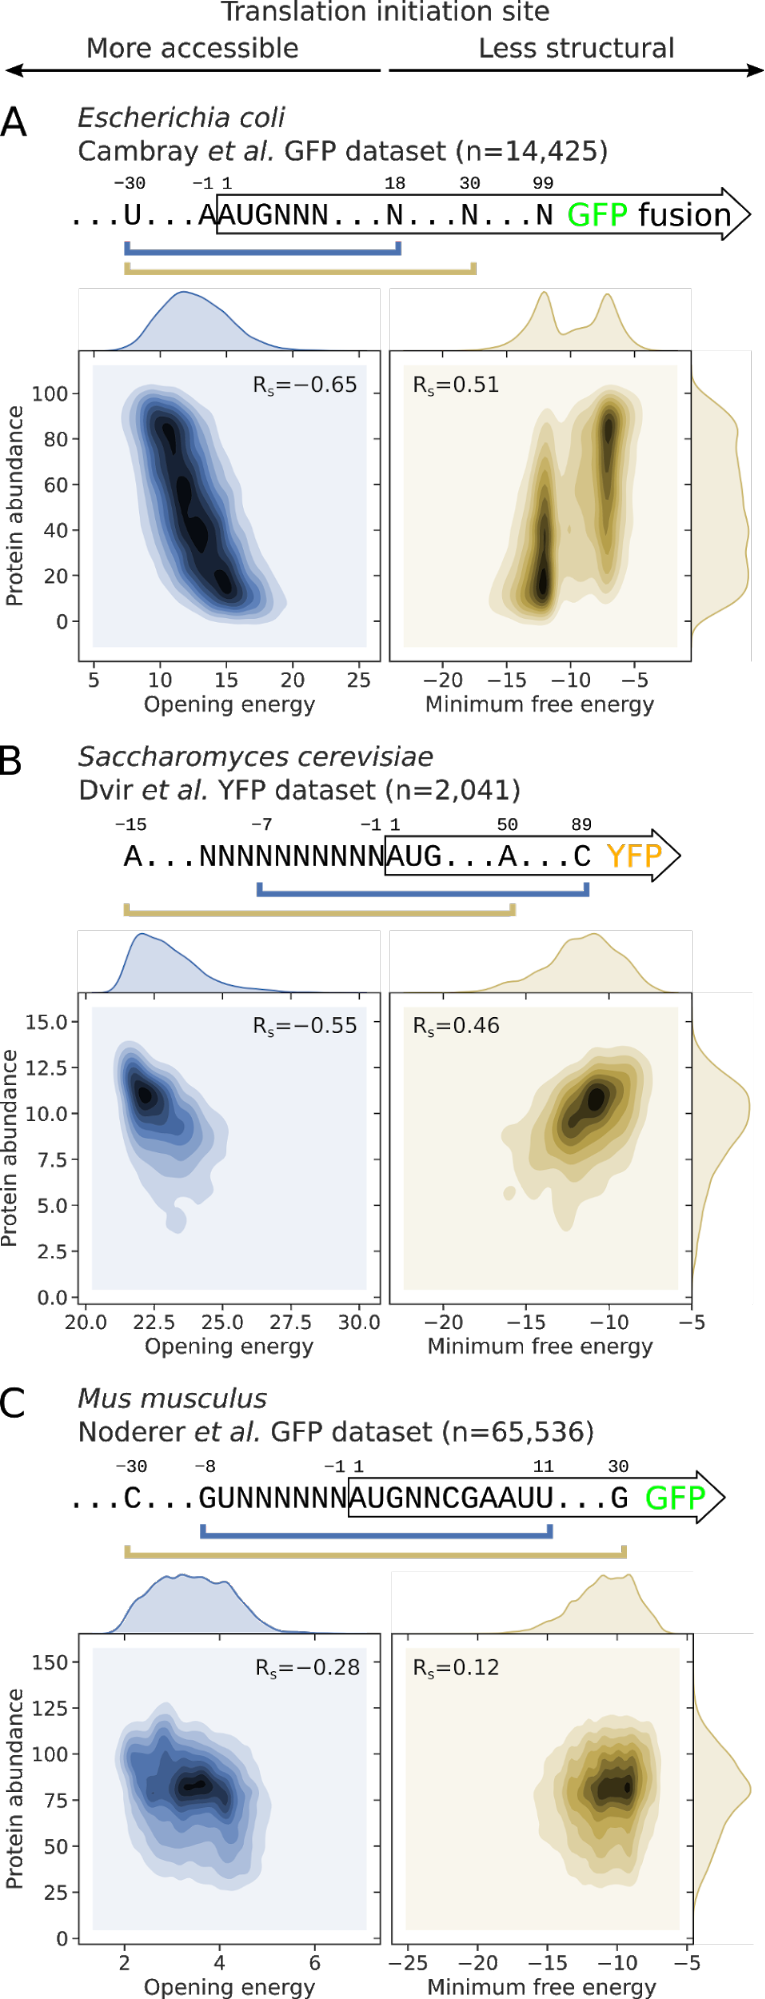
\includegraphics[width=0.5\textwidth]{chapters/TIsigner/Figs/fig1.png}
% \caption[Correlations between the opening energies of translation initiation sites and protein abundance are stronger than that of minimum free energy.]{\textbf{Correlations between the opening energies of translation initiation sites and protein abundance are stronger than that of minimum free energy. (A)}. For \textit{E. coli}, the opening energy at the region $−30:18$ shows the strongest correlation with protein abundance (see also \ref{fig:tisigner_fig2}B or Supplementary Fig S6A, sub-sequence l=48 at position i=18). For this analysis, we used a representative GFP expression dataset from Cambray et al. (2018). The reporter library consists of GFP fused in-frame with a library of 96-nt upstream sequences (N=14,425). The minimum free energy −30:30 shown was determined by Cambray et al. (right panel). \textbf{(B)}  For \textit{S. cerevisiae}, the opening energy $−7:89$ shows the strongest correlation with protein abundance (see also Supplementary Fig S6B, sub-sequence l=96 at position i= 89). For this analysis, we used the YFP expression dataset from Dvir et al. (2013). The YFP reporter library consists of 2,041 random decameric nucleotides inserted at the upstream of YFP start codon. The minimum free energy $−15:50$ was previously shown to correlate the best with protein abundance (right panel). \textbf{C} For \textit{M. musculus}, the opening energy $−8:11$ shows the strongest correlation with protein abundance (see also Supplementary Fig S6C, sub-sequence l=19 at position i=11). For this analysis, we used the GFP expression dataset from Noderer et al. (2014). The GFP reporter library consists of 65,536 random hexameric and dimeric nucleotides inserted at the upstream and downstream of GFP start codon, respectively. The minimum free energy −30:30 was shown (right panel). See also Supplementary Table S4. $R_s$, Spearman’s rho. Bonferroni adjusted P-values are below machine’s underflow level for the correlations between opening energies and protein abundances shown in the left panels.}
% \label{fig:tisigner_fig1}
% \end{SCfigure}

\begin{SCfigure}[][hbtp!]
	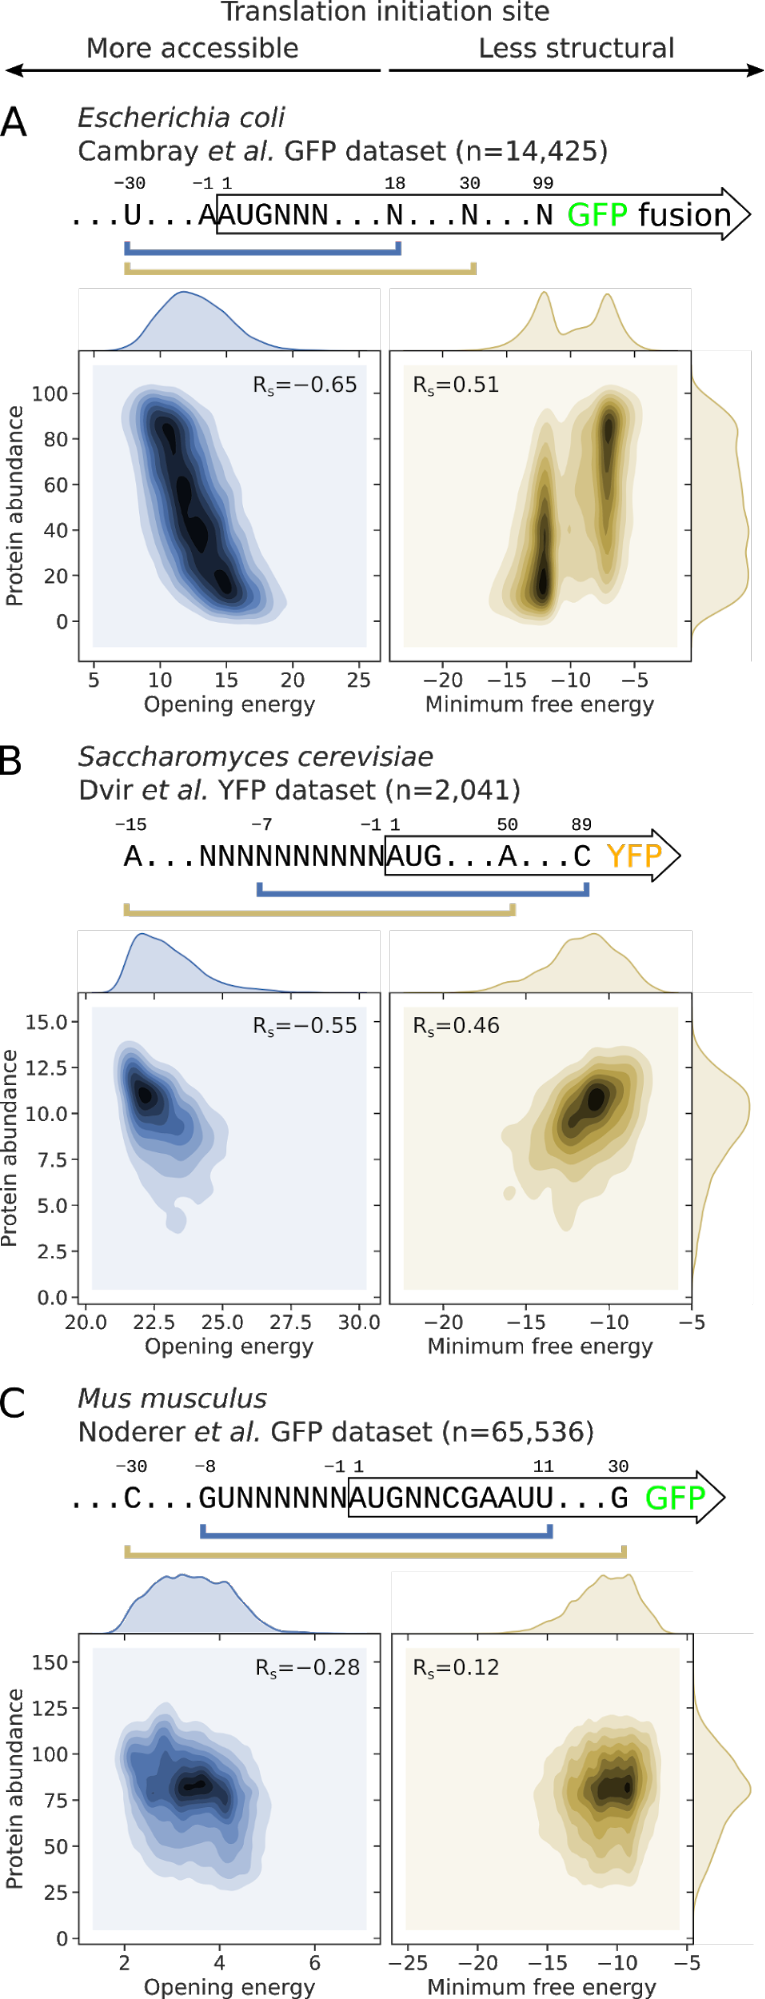
\includegraphics[width=0.5\textwidth]{chapters/TIsigner/Figs/fig1.png}
	\caption[Correlations between the opening energies of translation initiation sites and protein abundance are stronger than that of minimum free energy.]{\textbf{Correlations between the opening energies of translation initiation sites and protein abundance are stronger than that of minimum free energy. (A)}. For \textit{E. coli}, the opening energy at the region −30:18 shows the strongest correlation with protein abundance (see also \ref{fig:tisigner_fig2}B or Supplementary Fig S6A, sub-sequence l=48 at position i=18). For this analysis, we used a representative GFP expression dataset (N=14,425) from Cambray et al. (2018).The minimum free energy −30:30 shown was determined by Cambray et al. (right panel). \textbf{(B)}  For \textit{S. cerevisiae}, the opening energy −7:89 shows the strongest correlation with protein abundance (see also Supplementary Fig \ref{fig:appendix_TIsigner_S6}B, sub-sequence l=96 at position i= 89). For this analysis, we used the YFP expression dataset (N=2,041) from Dvir et al. (2013). The minimum free energy −15:50 was previously shown to correlate the best with protein abundance (right panel). \textbf{(C)} For \textit{M. musculus}, the opening energy −8:11 shows the strongest correlation with protein abundance (see also Supplementary Fig \ref{fig:appendix_TIsigner_S6}C, sub-sequence l=19 at position i=11). For this analysis, we used the GFP expression dataset (N=65,536) from Noderer et al. (2014). The minimum free energy −30:30 was shown (right panel). See also Supplementary Table S4. $R_s$, Spearman’s rho. Bonferroni adjusted P-values are below machine’s underflow level for the correlations between opening energies and protein abundances shown in the left panels.}
	\label{fig:tisigner_fig1}
\end{SCfigure}


We repeated the analysis for a dataset of yellow fluorescent protein (YFP) expression in \textit{Saccharomyces cerevisiae} \cite{Dvir2013-lq}. This dataset corresponds to a library of $5^{\prime}$ UTR variants, in which the 10-nt sequences preceding the YFP translation initiation site were randomly substituted (N=2,041 variants). In this case, the opening energy $−7:89$ showed a stronger correlation with protein abundance than that of the minimum free energy $−15:50$ reported previously (\ref{fig:tisigner_fig1}B; $R_s=−0.55$ versus $0.46$).

To examine the usefulness of accessibility in complex eukaryotes, we analysed a dataset of GFP expression in \textit{Mus musculus} \cite{Noderer2014-ve}. The reporter library was originally designed to measure the strength of translation initiation sequence context, in which all possible substitutions were made at the flanking regions of the GFP translation initiation site (6-nt upstream region and 2-nt downstream region of initiation codon; N=65,536 variants). Here the opening energy $−8:11$ showed a maximum correlation with expressed proteins, which again, is stronger than that of the minimum free energy $−30:30$ (\ref{fig:tisigner_fig1}C; $R_s=−0.28$ versus $0.12$). 

Taken together, our findings suggest that the accessibility of translation initiation sites strongly correlates with protein abundance across species. Interestingly, our findings also suggest that the Shine-Dalgarno sequence \cite{Shine1974-kl} at $−13:−8$ should be accessible to recruit ribosomes.

\subsection{Accessibility predicts the outcome of recombinant protein expression}
We investigated how accessibility performs in the real world in prediction of recombinant protein expression. For this purpose, we analysed 11,430 expression experiments in \textit{E. coli} from the ‘Protein Structure Initiative:Biology’ (PSI:Biology) \cite{Chen2004-cp,Seiler2014-on,Acton2005-ng}. These PSI:Biology targets were expressed using the pET21\_NESG expression vector that harbours the T7lac inducible promoter and a C-terminal His tag \cite{Acton2005-ng}.

We split the experimental results of the PSI:Biology targets into protein expression ‘success’ and ‘failure’ groups that were previously curated by DNASU (N=8,780 and 2,650, respectively; see Supplementary Fig \ref{fig:appendix_TIsigner_S7}). These PSI:Biology targets span more than 189 species and the failures are representative of various problems in heterologous protein expression. Only 1.6\% of the targets were \textit{E. coli} proteins, which is negligible (N=179; see Supplementary Fig \ref{fig:appendix_TIsigner_S7}).

We calculated the opening energies for all possible sub-sequences of the PSI:Biology targets as above (\ref{fig:tisigner_fig2}, positions relative to initiation codons). For each sub-sequence region, we used the opening energies to predict the expression outcomes and computed the prediction accuracy using the area under the receiver operating characteristic curve (AUC; see \ref{fig:tisigner_fig2}C). A closer look into the correlations between opening energies and expression outcomes, and AUC scores calculated for the sub-sequence regions reveals a strong accessibility signal of translation initiation sites (\ref{fig:tisigner_fig2}B and C, Cambray’s GFP and PSI:Biology datasets, respectively). We matched the correlations and AUC scores by sub-sequence regions and confirmed that sub-sequence regions that have strong correlations are likely to have high AUC scores (\ref{fig:tisigner_fig2}D). In contrast, the sub-sequence regions that have zero correlations are not useful for predicting the expression outcomes (AUC approximately 0.5).

We then asked how accessibility manifests in the endogenous mRNAs of \textit{E. coli}, for which we studied a proteomics dataset of 3,725 proteins available from PaxDb \cite{Wang2015-ky}. As expected, we observed a similar accessibility signal, with the region −25:16 correlated the most with protein abundance (\ref{fig:tisigner_fig2}E). However, the correlation was rather low ($R_s=−0.17$, $P<2.2 \times 10^{-16}$), which may reflect the limitation of mass spectrometry to detect lower abundances \cite{Tabb2009-ek,Nilsson2010-ol}. Furthermore, the endogenous promoters have variable strength, which gives rise to a broad range of mRNA and protein levels \cite{Deuschle1986-oz,Delvigne2017-vm}. Taken together, our results show that the accessibility signal of translation initiation sites is very consistent across various datasets analysed (Supplementary Fig \ref{fig:appendix_TIsigner_S6} and \ref{fig:tisigner_fig2}).


\begin{SCfigure}[][hbtp!]
	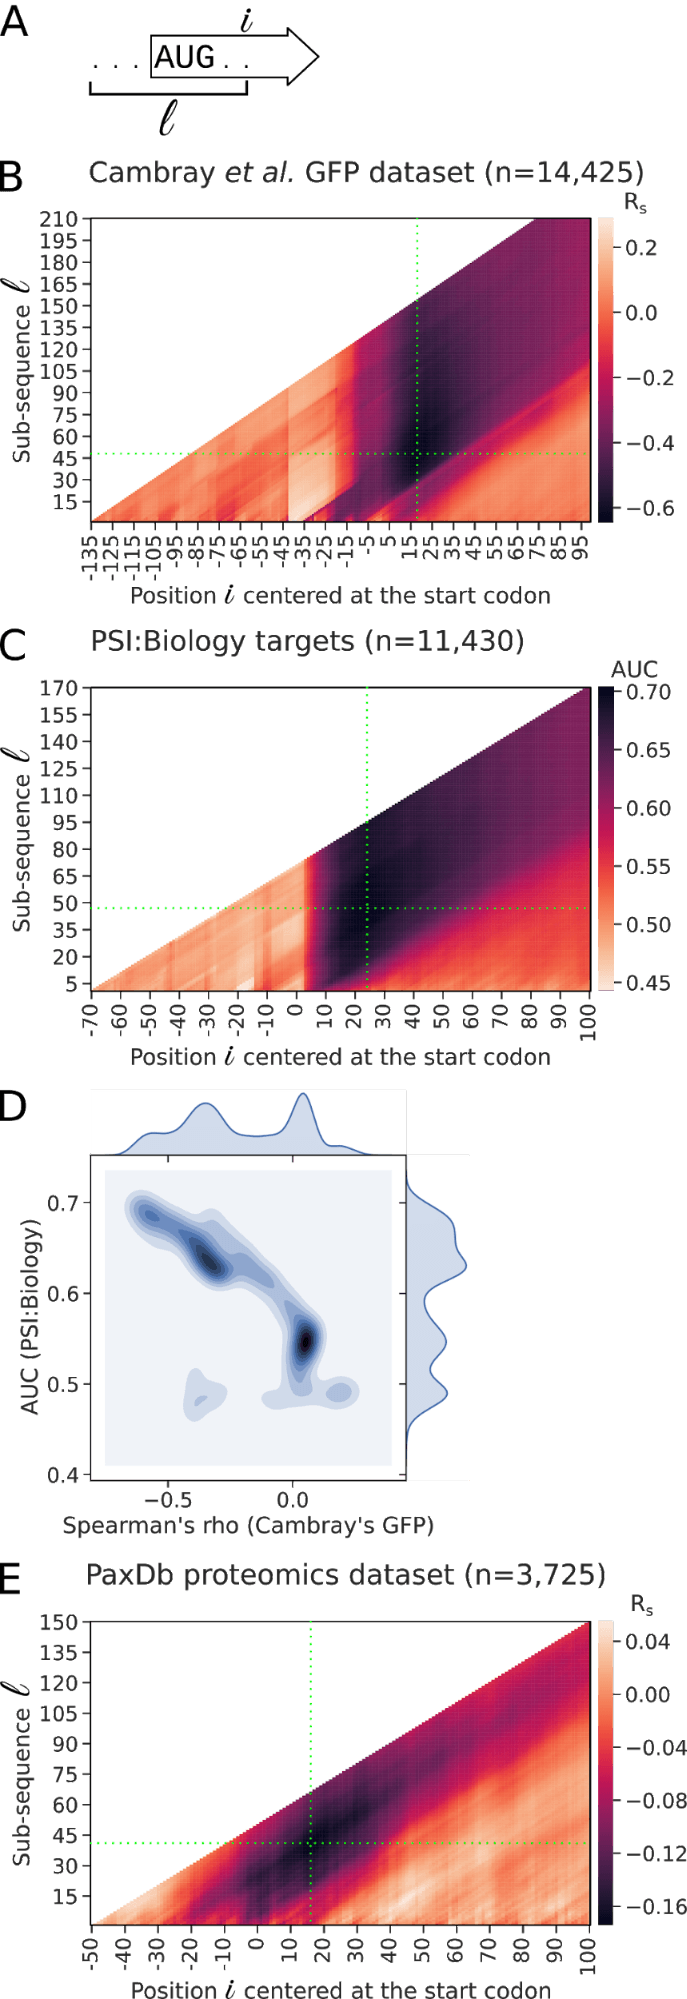
\includegraphics[width=0.5\textwidth]{chapters/TIsigner/Figs/fig2.png}
	\caption[Opening energies of regions surrounding the Shine-Dalgarno and start codons are predictive of protein expression in \textit{E. coli}.]{\textbf{Opening energies of regions surrounding the Shine-Dalgarno and start codons are predictive of protein expression in \textit{E. coli}. (A)} Schematic representation of a transcript sub-sequence l at position i for the calculation of opening energy. \textbf{(B)} Correlation between the opening energies for the sub-sequences of GFP transcripts and protein abundance. The opening energy at the region −30 to 18 nt (green crosshair) shows the strongest correlation with protein abundance [$R_s=−0.65$; N=14,425, GFP expression dataset of Cambray et al. (2018)]. \textbf{(C)} Prediction accuracy of the expression outcomes of the PSI:Biology targets using opening energy (N=11,430). The opening energy at the region −23:24 (green crosshair) shows the highest prediction accuracy score (AUC=0.70). \textbf{(D)} Comparison between the correlations and AUC scores by sub-sequence region taken from the above analyses. Sub-sequences that have strong correlations are likely to have high AUC scores, whereas the sub-sequence regions that have no correlations are likely not useful in prediction of the expression outcomes. \textbf{(E)} Correlation between the opening energies for the sub-sequences of \textit{E. coli} transcripts and protein abundance. The transcripts used for this analysis are protein-coding sequences concatenated with 50 and 10 nt located upstream and downstream, respectively. The opening energy at the region −25:16 (green crosshair) shows the strongest correlation with protein abundance ($R_s=−0.17$; N=3,725, PaxDb integrated proteomics dataset). See also Supplementary Table S4. $R_s$, Spearman’s rho. }
	\label{fig:tisigner_fig2}
\end{SCfigure}




\subsection{Accessibility outperforms other features in prediction of recombinant protein expression}
To choose an accessibility region for subsequent analyses, we selected the top 200 regions from the above correlation analysis on Cambray’s GFP dataset (\ref{fig:tisigner_fig2}B) and used random forest to rank their Gini importance scores in prediction of the outcomes of the PSI:Biology targets. The region $−24:24$ was ranked first, which is nearly identical to the region $−23:24$ with the top AUC score (\ref{fig:tisigner_fig2}C, AUC=0.70). We therefore used the opening energy at the region $−24:24$ in subsequent analyses.

We asked how the other features perform compared to accessibility in prediction of heterologous protein expression, for which we analysed the same PSI:Biology dataset. We first calculated the minimum free energy and avoidance at the regions −30:30 and 1:30, respectively. These are the local features associated with translation initiation rate. We also calculated CAI \cite{Sharp1987-ed}, tAI \cite{Tuller2010-ub}, codon context (CC) \cite{Ang2016-rv}, G+C content, and I$\chi$nos scores \cite{Tunney2018-sr}. CC is similar to CAI except it takes codon-pairs into account, whereas the I$\chi$nos scores are translation elongation rates predicted using a neural network model trained with ribosome profiling data (Supplementary Fig \ref{fig:appendix_TIsigner_S8}). These are the global features associated with translation elongation rate. We built a random forest model to rank the Gini importance scores of these local and global features. The local features ranked higher than the global features (\ref{fig:tisigner_fig3}A). We then calculated and compared the prediction accuracy of these features. The AUC scores for the local features were 0.70, 0.67 and 0.62 for the opening energy, minimum free energy and avoidance, respectively, whereas the global features were 0.58, 0.57, 0.54, 0.54 and 0.51 for I$\chi$nos, G+C content, CAI, CC and tAI, respectively (\ref{fig:tisigner_fig3}B). The local features outperform the global features, suggesting that effects on translation initiation are a major predictor of the outcome of heterologous protein expression. We further examined the local G+C contents corresponding to the local features (Supplementary Fig \ref{fig:appendix_TIsigner_S9}). The G+C contents in the regions $−24:24$ and $−30:30$ weakly correlate with opening energy and minimum free energy, respectively. The AUC scores for these local G+C contents are also lower than the corresponding local features, suggesting that these local G+C contents are not good proxies for the corresponding local features. Overall, our findings support previous reports that the effects on translation initiation are rate-limiting \cite{Kudla2009-tl,Tuller2015-ts} which, interestingly, correlate with the binary outcome of recombinant protein expression (\ref{fig:tisigner_fig3}C). Importantly, accessibility outperformed all other features.


\begin{figure}[hbtp!]
	\center
	\includegraphics[width=1\textwidth]{chapters/TIsigner/Figs/fig3.png}
	\caption[Accessibility of translation initiation sites is the strongest predictor of heterologous protein expression in \textit{E. coli}.]{\textbf{Accessibility of translation initiation sites is the strongest predictor of heterologous protein expression in \textit{E. coli}. (A)} mRNA features ranked by Gini importance for random forest classification of the expression outcomes of the PSI:Biology targets (N=8,780 and 2,650, ‘success’ and ‘failure’ groups, respectively). The features associated with translation initiation rate (purple; opening energy −24:24, minimum free energy −30:30, and mRNA:ncRNA avoidance 1:30) have higher scores than the feature associated with translation elongation rate [blue; tRNA adaptation index (tAI), codon context (CC), codon adaptation index (CAI), G+C content (\%), and I$\chi$nos]. The I$\chi$nos scores are translation elongation rates predicted using a neural network model trained with ribosome profiling data (Supplementary Fig \ref{fig:appendix_TIsigner_S8}). \textbf{(B)} ROC analysis shows that accessibility (opening energy −24:24) has the highest classification accuracy. The AUC scores with 95\% confidence intervals are shown. See also Supplementary Table S4. \textbf{(C)} Accessibility (opening energy −24:24) is the best feature in explaining the expression outcomes.  $R_s$, Spearman’s rho. }
	\label{fig:tisigner_fig3}
\end{figure}




To identify a good opening energy threshold, we calculated positive likelihood ratios for different opening energy thresholds using the cumulative frequencies of true negative, false negative, true positive and false positive derived from the above receiver operating characteristic (ROC) analysis (Supplementary Fig \ref{fig:appendix_TIsigner_S12}, top panel). Meanwhile, we calculated the 95\% confidence intervals of these positive likelihood ratios using 10,000 bootstrap replicates. We reasoned that there is an upper and lower bound on translation initiation rate, therefore the relationship between translation initiation rate and accessibility is likely to follow a sigmoidal pattern. We fit the positive likelihood ratios into a four-parametric logistic regression model (Supplementary Fig \ref{fig:appendix_TIsigner_S12}). As a result, we are 95\% confident that an opening energy of 10 kcal/mol or below at the region $−24:24$ is about two times more likely to belong to the sequences which are successfully expressed than those that failed.

\subsection{Accessibility can be improved using a simulated annealing algorithm}
The above results suggest that accessibility can, in part, explain the low expression problem of heterologous protein expression. Therefore, we sought to exploit this idea for optimising gene expression. We developed a simulated annealing algorithm to maximise the accessibility at the region $−24:24$ using synonymous codon substitution (see Methods). Previous studies have found that full-length synonymous codon-substituted transgenes may produce unexpected results, such as a reduction in mRNA abundance, RNA toxicity, and/or protein misfolding \cite{Ben-Yehezkel2015-bj,Umu2016-zq,Tunney2018-sr,mittal2018codon}. Therefore, we sought to determine the minimum number of codons required for synonymous substitutions in order to achieve near-optimum accessibility. For this purpose, we used the PSI:Biology targets that failed to be expressed. We applied our simulated annealing algorithm such that synonymous substitutions can happen at any codon of the sequences except the start and stop codons, although the changes may not necessarily happen to all codons due to the stochastic nature of our optimisation algorithm (see Methods).  Next, we constrained synonymous codon substitution to the first 14 codons and applied the same procedure (Supplementary Fig \ref{fig:appendix_TIsigner_S10}A). Therefore, the changes may only occur at any or all of the first 14 codons. We repeated the same procedure for the first nine and also the first four codons. Thus a total of four series of codon-substituted sequences were generated. We then compared the distributions of opening energy −24:24 for these series using the Kolmogorov-Smirnov statistic (DKS; see Supplementary Fig \ref{fig:appendix_TIsigner_S10}B). The distance between the distributions of the nine and full-length codon-substituted series was significantly different yet sufficiently close (DKS=0.087, P=$3.3 \times 10^{-8}$), suggesting that optimisation of the first nine codons is sufficient in most cases to achieve an optimum accessibility of translation initiation sites. We named our software Translation Initiation coding region designer (TIsigner), which by default, allows synonymous substitutions in the first nine codons.

We asked to what extent the existing gene optimisation tools modify the accessibility of translation initiation sites. For this purpose, we first submitted the PSI:Biology targets that failed to be expressed to the ExpOptimizer web server from NovoPro Bioscience (see Methods). We also optimised the PSI:Biology targets using the standalone version of Codon Optimisation OnLine (COOL) \cite{Chung2012-zh}. We found that both tools increase accessibility indirectly even though their algorithms are not specifically designed to do so. In fact, a purely random synonymous codon substitution on these PSI:Biology targets using our own script resulted in similar increases in accessibility (Supplementary Fig \ref{fig:appendix_TIsigner_S10}C). These results may explain some indirect benefits from the existing gene optimisation tools (i.e. any change from suboptimal is likely to be an improvement, see below).

\subsection{Low protein yields can be improved by synonymous codon changes in the vicinity of translation initiation sites}
To demonstrate that heterologous protein expression is tunable with minimum effort, we designed and tested a series of GFP reporter gene constructs. We tested 29 plasmids harbouring GFP reporter genes with synonymous changes within the first nine codons (opening energies from 5.56 to 21.68 kcal/mol; Supplementary Table S5 and Supplementary Methods). GFP expression is controlled by an IPTG inducible T7lac promoter. In addition, all plasmids harbour a second reporter gene, i.e. mScarlet-I, which is controlled by the constitutive promoter from the nptII gene for aminoglycoside-3'-O-phosphotransferase of E. coli transposon Tn5 \cite{Bindels2017-ud,Schlechter2018-nj}. mScarlet-I expression was measured to correct for plasmid copy number and as a proxy for bacterial growth \cite{Schlechter2020-ab}. 

Consistent with the above results, the GFP level significantly correlates with accessibility (i.e., anti-correlates with opening energy, $R_s=−0.53$, $P=3.4\times 10^{-3}$; \ref{fig:tisigner_fig4}A). This correlation was also the strongest compared to other features. Curiously, we observed a diminishing return with opening energies lower than that of the wild-type sequence (11.68 kcal/mol). To investigate this, we simulated a protein production experiment by modelling cell growth, transcription, translation, and turnovers (see Methods). We assumed that opening energies of 12 kcal/mol or below is favourable in this model, based on our analysis of 8,780 PSI:Biology 'success' group (Supplementary Fig \ref{fig:appendix_TIsigner_S10}). Interestingly, our in silico coarse-grained model shows a similar protein production trend as the actual experiment (\ref{fig:tisigner_fig4}B).

We then tested this finding using the luciferase reporter of \textit{Renilla reniformis} (RLuc). Similarly, we designed a series of RLuc variants, but with opening energies below that of the wild-type sequence (5.77 to 10.38 kcal/mol; Supplementary Fig S13 and Table S5). In addition, we tested commercially designed sequences, in which sequence optimisations were performed in full-length rather than the first 9 codons. However, RLuc is poorly soluble in the BL21Star(DE3) \textit{E. coli} host (Supplementary Fig \ref{fig:appendix_TIsigner_S13}B). We observed that TIsigner (9.9 kcal/mol) and commercially optimised luciferase reporter genes produced significantly higher luminescence than the wild-type. We also found that the levels of wild-type luciferase and many variants with lower opening energies (5-7 kcal/mol) were not significantly different, likely due to poor solubility.

\begin{SCfigure}[][hbtp!]
	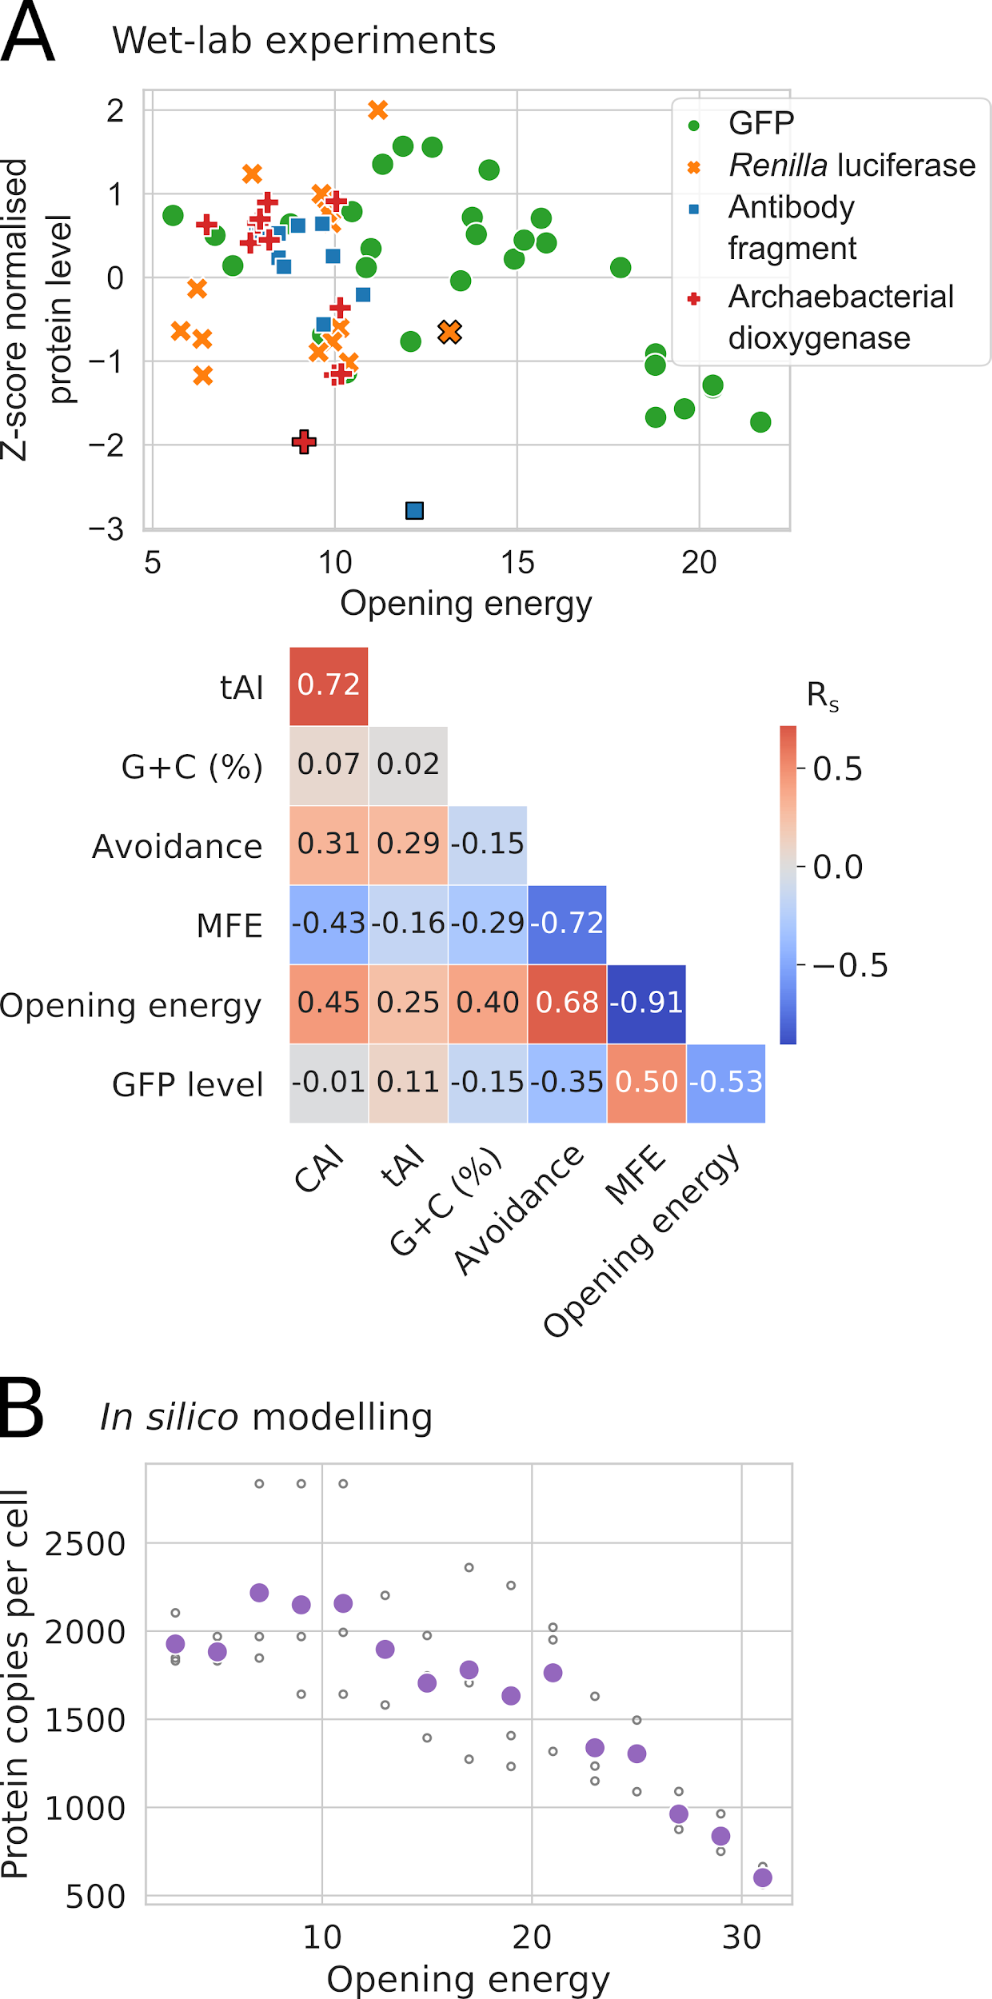
\includegraphics[width=0.5\textwidth]{chapters/TIsigner/Figs/fig4.png}
	\caption[The yields of heterologous protein productions are tunable by synonymous codon changes in the first nine codons.]{\textbf{The yields of heterologous protein productions are tunable by synonymous codon changes in the first nine codons. (A)} GFP level strongly correlates with accessibility, i.e., anti-correlates with opening energy ($R_s=−0.53$, $P=3.4 \times 10^{−3}$; N=29). This correlation is the strongest compared to other features. The protein levels of GFP, \textit{Renilla} luciferase (RLuc), an antibody fragment and an archaebacterial dioxygenase were transformed using z-score method. The GFP and RLuc levels were derived from the average values of at least two and three independent biological replicates, respectively. Black outlines denote wild-type sequences. See also Supplementary Fig \ref{fig:appendix_TIsigner_S13}, \ref{fig:appendix_TIsigner_S14} and Table S5. CAI, codon adaptation index; CC, codon context; Rs, Spearman’s rho; tAI, tRNA adaptation index. \textbf{(B)} Coarse-grained simulation of a protein production experiment by modelling cell growth, transcription, translation, and turnovers, given that translation initiation sites with opening energies less than or equal to 12 kcal/mol is optimum. The in silico model shows a similar trend of protein production as the wet-lab experimental results. Unfilled and filled (purple) circles denote the in silico replicates and their corresponding average values, respectively ($R_s=−0.75$, $P=2.8\times 10^{−9}$).}
	\label{fig:tisigner_fig4}
\end{SCfigure}



As both wild-type GFP and RLuc genes are strongly expressed in \textit{E. coli}, we asked whether poorly expressed proteins can be improved by increasing accessibility of translation initiation sites. We performed densitometric analysis of previously published Western blots, which include the results of a cell-free expression system using constructs harbouring a wild-type antibody fragment or archaebacterial dioxygenase and its synonymous variants (within the first six codons) \cite{Voges2004-dt}. Indeed, variants with opening energies lower than the wild-type sequences were expressed at higher levels (Supplementary Fig \ref{fig:appendix_TIsigner_S14}).

\section{Discussion}
Our findings show that the accessibility of translation initiation sites is the strongest predictor of heterologous protein expression in E. coli. Whereas previous studies have largely used minimum free energy models to define the accessibility of a region of interest \cite{Salis2009-dh,Bhattacharyya2018-zy,Nieuwkoop2019-ft,Voges2004-dt,pelletier1987involvement}. However, Terai and Asai (2020) and ourselves have independently discovered that the opening energy is a better choice for modelling accessibility \cite{Bhandari2021-wd,Terai2020-co} (see \ref{fig:tisigner_fig1}A for example). Opening energy is an ensemble average energy that accounts for suboptimal RNA structures that are not reported by minimum free energy models by default \cite{Muckstein2006-ys,Bernhart2011-cc}. Currently, the modelling of accessibility using opening energy is largely used for the prediction of RNA-RNA intermolecular interactions, for example, as implemented in RNAup and IntaRNA \cite{Lorenz2011-rg,Mann2017-yy}. Our study has shown that this approach can be used to identify the key accessibility regions that are consistent across multiple large expression datasets. We have implemented our findings in TIsigner web server, which currently supports recombinant protein expression in \textit{E. coli} and \textit{S. cerevisiae} (optimisation regions $−24:24$ and $−7:89$, respectively; see \ref{fig:tisigner_fig1}). An independent yet similar implementation is available in XenoExpressO web server with the purpose of optimising protein expression for an \textit{E. coli} cell-free system \cite{Zayni2018-wc}. The authors showed that an increase in accessibility of a 30 bp region from the Shine-Dalgarno sequence enhances the expression level of human voltage dependent anion channel, which further supports our findings.

The strengths of our approaches are five-fold. Firstly, the likelihood of success or failure can be assessed prior to running an experiment. Users can compare the opening energies calculated for the input and optimised sequences and the distributions of the ‘success’ and ‘failure’ of the PSI:Biology targets. We also introduced a scoring scheme to score the input and optimised sequences based upon how likely they are to be expressed (Supplementary Fig \ref{fig:appendix_TIsigner_S12}; see also Methods). Secondly, optimised sequences can have up to the first nine codons substituted (by default), meaning that gene optimisation using a standard PCR cloning method is feasible. For cloning, we propose a nested PCR approach, in which the final PCR reaction utilises a forward primer designed according to the optimised sequence \cite{Sambrook2001-ki} (Supplementary Fig \ref{fig:appendix_TIsigner_S10}D). Thirdly, the cost of gene optimisation can be reduced dramatically as gene synthesis is replaced with PCR using our approach. This enables high-throughput protein expression screening using the optimised sequences, generated at a low cost. Fourthly, tunable expression is possible, i.e. high, intermediate or even low expression $5^{\prime}$ codon sequences can be designed, allowing for more control over heterologous protein production, as demonstrated by our experiments (\ref{fig:tisigner_fig4}). Finally, our fast, lightweight, coarse-grained simulation approach has opened up new avenues to study several aspects of gene expression, such as transcription, translation, cellular growth, and turnovers, which give good proxies to how cellular systems behave.


\section{Material and methods}
\subsection{Plasmids}
Plasmids were constructed using the MIDAS Golden Gate cloning system (see Supplementary Methods, Fig \ref{fig:appendix_TIsigner_S1}, \ref{fig:appendix_TIsigner_S2}, \ref{fig:appendix_TIsigner_S3}, \ref{fig:appendix_TIsigner_S4}, \ref{fig:appendix_TIsigner_S5}, and Table \ref{tab:appendix_TIsigner_T1}, \ref{tab:appendix_TIsigner_T2}, \ref{tab:appendix_TIsigner_T3}) \cite{Van_Dolleweerd2018-sg}.

\subsection{Data}
Datasets used in this study are listed in Supplementary Table S4. These include fluorescence reporter expression datasets previously generated using E. coli, Saccharomyces cerevisiae, and Mus musculus cultured cells (Supplementary Fig \ref{fig:appendix_TIsigner_S6}), and recombinant protein production dataset from the Protein Structure Initiative: Biology (PSI:Biology; Supplementary Fig \ref{fig:appendix_TIsigner_S7}). Two ribosome profiling libraries previously generated using \textit{E. coli} were retrieved from the Sequence Read Archive (SRR7759806 and SRR7759807) \cite{Mohammad2019-if}.

\subsection{Sequence features analysis}
Representative sequences were chosen using CD-HIT-EST \cite{Li2006-qp,Fu2012-ng}. Minimum free energies, opening energies and avoidance were calculated using RNAfold, RNAplfold and RNAup from ViennaRNA package (version 2.4.11), respectively \cite{Hofacker1994-vu,Muckstein2006-ys,Bernhart_undated-tw,Bompfunewerer2008-tm,Lorenz2011-rg,Bernhart2011-cc,Lorenz2016-ie}. RNAfold was run with default parameters. For RNAplfold, sub-sequences were generated from the input sequences to calculate opening energies (using the parameters -W 210 -u 210). For RNAup, we examined the stochastic interactions between the region 1:30 of each mRNA and 54 non-coding RNAs (using the parameters -b -o). RNAup reports the total interaction between two RNAs as the sum of energy required to open accessible sites in the interacting molecules Gu and the energy gained by subsequent hybridisation Gh\cite{Muckstein2006-ys}. For the interactions between each mRNA and 54 non-coding RNAs, we chose the most stable mRNA:ncRNA pair to report an inappropriate mRNA:ncRNA interaction, i.e. the pair with the strongest hybridisation energy, (Gh)min. 

CAI, tAI and Codon Context (CC) were calculated using the reference weights from Sharp and Li \cite{Sharp1987-ed}, Tuller et al. \cite{Tuller2010-ub} and Ang et al. \cite{Ang2016-rv}, respectively. Translation elongation rate was predicted using I$\chi$nos \cite{Tunney2018-sr} that were trained using the \textit{E. coli} ribosome profiling data (Supplementary Fig \ref{fig:appendix_TIsigner_S8}). Local G+C contents were also examined (Supplementary Fig \ref{fig:appendix_TIsigner_S9}).

\subsection{Coarse-grained simulation}
To understand the dynamics between accessibility and protein production, we performed a coarse grained simulation using constructs with increasing opening energy on a simulated cellular system. Despite being less precise than fine grained methods such as ab initio and molecular dynamics, coarse grained simulations often give similar results, with an added advantage of being scalable to very large systems.

To set the simulation, we binned the opening energies between 2 and 32 in intervals of two, with each bin representing a ‘reporter plasmid construct’ whose opening energy is the mean of the bin. For each construct, the ‘technical replicates’ were generated by allowing slight variations on the mean opening energy of the bin. This is to model variation between replicates, and the discrepancies between the estimated and the actual opening energies in vivo. For each round of transcription, mRNA copies were randomly generated from 30 to 60 plasmid DNA copies \cite{Held2003-ts,Gomes2020-ek,Rosano2014-oq}. We chose an optimum opening energy of 12 kcal/mol or less for translation (Supplementary Fig \ref{fig:appendix_TIsigner_S10}). However, this is probabilistic which occasionally allowed protein production from higher opening energy transcripts. We allowed mRNA to decay probabilistically when a mRNA molecule is translated for more than 10 rounds.

We also set a threshold of protein tolerance to be 1,000,000 copies where the copy numbers of endogenous proteins are usually less than 10,000 \cite{Taniguchi2010-uq}, beyond which there is a sporadic death of cells. However, in this simulation, the chances of staying viable and reproducing are higher than death, and cells grow steadily. This threshold also simulated random but low cell deaths in the experiment, without setting an extra variable.

To limit the computational complexity, our coarse-grained simulations used lower constants and iterations. Initialising with 100 cells, the algorithm was set to terminate either after 10,000 iterations or when the total number of  cells becomes zero. After termination, the total number of proteins and cells for each construct were taken from the endpoints. To imitate ‘biological replicates’, we repeated the above simulation three times with different random numbers, which provides slightly different initial conditions for each experiment.

\subsection{Development of Translation Initiation coding region designer (TIsigner)}
Finding a synonymous sequence with a maximum accessibility is a combinatorial problem that spans a vast search space. For example, for a protein-coding sequence of nine codons, assuming an average of 3 synonymous codons per amino acid, we can expect a total of 19,682 unique synonymous coding sequences. This number increases rapidly with increasing numbers of codons. Heuristic optimisation approaches are preferred in such situations because the search space can be explored more efficiently to obtain nearly optimal solutions. 

To optimise the accessibility of a given sequence, TIsigner uses a simulated annealing algorithm \cite{Kirkpatrick1983-hh,Ingber2000-aw,Keith2002-jx,Brownlee2011-bk}, a heuristic optimisation technique based on the thermodynamics of a system settling into a low energy state after cooling. Simulated annealing algorithms have been used to solve many combinatorial optimisation problems in bioinformatics. For example, we previously applied this algorithm to align and predict non-coding RNAs from multiple sequences \cite{Lindgreen2007-jy}. Other studies use this algorithm to find consensus sequences \cite{Keith2002-jx}, optimise ribosome binding sites \cite{Salis2009-dh} and predict mRNA foldings \cite{Gaspar2013-bg} using minimum free energy models.

% According to statistical mechanics, the probability pi of a system occupying energy state Ei,with temperatureT, follows a Boltzmann distribution of the form e-Ei/T, which gives a set of probability mass functions along every point i in the solution space.  Using a Markov chain sampling, these probabilities are sampled such that each point has a lower temperature than the previous one. As the system is cooled from high to low temperatures (T0), the samples converge to a minimum of E, which in many cases will be the global minimum \cite{Keith2002-jx}. A frequently used Markov chain sampling technique is Metropolis-Hastings algorithm in which a ‘bad’ moveE2 from initial state E1 such that E2 >E1, is accepted if  R(0,1)  p2/ p1, where R(0,1) is a uniformly random number between 0 and 1.

In our implementation, each iteration consists of a move that may involve multiple synonymous codon substitutions. The algorithm begins at a high temperature where the first move is drastic, synonymous substitutions occur in all replaceable codons. At the end of the first iteration, a new sequence is accepted if the opening energy is smaller than that of the input sequence. However, if the opening energy of a new sequence is greater than that of the input sequence, acceptance depends on the Metropolis-Hastings criteria. The accepted sequence is used for the next iteration, which repeats the above process. As the temperature cools, the moves get milder with fewer synonymous codon changes (Supplementary Fig \ref{fig:appendix_TIsigner_S10}). Simulated annealing stops upon reaching a near-optimum solution. 

For the web version of TIsigner, the default number of replaceable codons is restricted to the first nine codons. However, this default setting can be reset to range from the first four to nine codons, or the full length of the coding sequence. Since the accessibility of a fixed region is optimised, this process only takes O(1) time (Supplementary Fig \ref{fig:appendix_TIsigner_S11}). Furthermore, TIsigner runs multiple simulated annealing instances, in parallel, to obtain multiple possible sequence solutions.

When users select T7lac promoter as the $5^{\prime}$ UTR, they can adjust ‘Expression Score’, that is calculated based on the PSI:Biology dataset (see below). This allows them to tune the expression level of a target gene. In contrast, when users input a custom $5^{\prime}$ UTR sequence, they only have the option to either maximise or minimise expression.

To implement ‘Expression Score’, the posterior probabilities of success for input and optimised sequences are evaluated using the following equations from Bayesian statistics:

\begin{equation*}
\begin{split}
positive\ posterior\ odds &= prior\ odds \times fitted\ positive\ likelihood\ ratio \\
positive\ posterior\ probability &= \frac{ positive\ posterior\ odds}{1 + positive posterior odds}
\end{split}
\end{equation*}


The fitted positive likelihood ratios were obtained from the following 4-parametric logistic regression equation:
\begin{equation*}
fitted\ positive\ likelihood\ ratio = d + \frac{(a-d)}{1+(\frac{positive\ likelihood\ ratio}{c})^b}
\end{equation*}

with parameters a, b, c, and d. The prior probability was set to 0.49, which is the proportion of ‘Expressed’ (N=21,046) divided by ‘Cloned’ (N=42,774) of the PSI:Biology targets reported as of 28 June 2017 (http://targetdb.rcsb.org/metrics/). Posterior probabilities were scaled as percentages to score the input and optimised sequences (Supplementary Fig \ref{fig:appendix_TIsigner_S12}).

The presence of terminator-like elements \cite{Chen2013-um} in the protein-coding region may result in expression of truncated mRNAs due to early transcription termination. Therefore, we implemented an optional check for putative terminators in the input and optimised sequences by cmsearch (INFERNAL version 1.1.2) \cite{Nawrocki2013-te} using the covariance models of terminators from RMfam \cite{Gardner2015-ui,Kalvari2018-un}. We also allow users to filter the output sequences for the presence of restriction sites. Restriction modification sites (AarI, BsaI, and BsmBI) are avoided by default.

Besides \textit{E. coli}, users can choose \textit{S. cerevisiae}, \textit{M. musculus} or ‘Other’ as the expression host. The regions for optimising accessibility are $−7:89$, $−8:11$ and $−24:89$ for \textit{S. cerevisiae}, \textit{M. musculus} and ‘Other’, respectively (\ref{fig:tisigner_fig1} and Supplementary Fig \ref{fig:appendix_TIsigner_S6}). When users choose ‘Custom’ for expression host, the region for optimising accessibility becomes customisable.

\subsection{Sequence optimisation}
We submitted the PSI:Biology targets that failed to be expressed (N=2,650) to the ExpOptimizer web server from NovoPro Bioscience (https://www.novoprolabs.com/\\tools/codon-optimization). A total of 2,573 sequences were optimised. The target sequences were also optimised using a local version of COOL \cite{Chung2012-zh} and TIsigner using default settings. We also ran a random synonymous codon substitution as a control for these 2,573 sequences.

\subsection{GFP assay}
BL21(DE3)pLysS competent \textit{E. coli} cells (Invitrogen) were transformed with plasmids and grown overnight on Luria-Bertani (LB) agar plates containing spectinomycin (50 $\mu g/ml$) and chloramphenicol (25 $\mu g/ml$). Single colonies were picked and inoculated into 3 ml LB broth containing the same antibiotics, and cultures were grown for 18 hours at 37$^{\circ}$C, 200 rpm. Cultures were diluted with fresh media at 1:20 and grown at 37$^{\circ}$C, 200 rpm, until reaching the mid-logarithmic growth phase (optical densities at 600 nm ($OD_{600}$) of ~0.3). Of each culture, 20 $\mu l$ was seeded into 96-well plates containing 180 $\mu l$  LB broth supplemented with antibiotics and isopropyl-$\beta$-D thiogalactopyranoside (IPTG) (1 mM final concentration) per well. Fluorescence intensities and ODs were measured in a black, flat, clear bottom 96-well plate with lid (CELLSTAR, Greiner) using a FLUOstar Omega plate reader (BMG Labtech) equipped with an excitation filter (band pass 485-12) and an emission filter (band pass 520) for GFP and excitation filter (band pass 484) and an emission filter (band pass 610-10) for mScarlet-I. The plate was incubated at 37$^{\circ}$C with “meander corner well shaking” at 300 rpm for 7 hours measuring fluorescence and ODs every 10 minutes. Fluorescence was measured in a 2 mm circle recording the average of 8 measurements per well. Average values of technical replicates were calculated and normalised to the mScarlet-I second reporter, and then to the normalised value of the GFP variant with the highest opening energy (21.68 kcal/mol). Normalised fluorescence values were obtained from the average values of biological replicates (Supplementary Fig \ref{fig:appendix_TIsigner_S13} and Table S5).

\subsection{Luciferase assay}
BL21Star(DE3) competent cells (Invitrogen) were transformed with plasmids and grown overnight at 37$^{\circ}$C on LB agar plates containing 50 $\mu g/ml$ spectinomycin. Single colonies were picked and inoculated into 5 ml LB broth (50 $\mu g/ml$ spectinomycin) and grown for 18 hours at 37$^{\circ}$C, 200 rpm. Bacterial cultures were diluted with fresh media at 1:20 and grown at 37$^{\circ}$C, 200 rpm, up to a mid-logarithmic phase ($OD_{600}$ of ~0.4). The cultures were split and induced with IPTG at a final concentration of 0.25 mM (or uninduced as controls), and seeded into a white, flat, clear bottom 96-well white plate with lid (Costar, Corning), 150 $\mu l$ per well, in triplicates. Cells were incubated in a FLUOstar Omega Microplate Reader (BMG LABTECH) for 90 minutes at 25$^{\circ}$C, 200 rpm, and $OD_{600}$ was measured every 15 minutes (over 7 cycles). Cells were harvested by centrifugation at $3000 \times g$, for 10 minutes, at 20$^{\circ}$C. Supernatants were removed. As the substrate can penetrate into cells, 50 $\mu l$ of coelenterazine h (Promega) was added to living cells to minimise sample processing steps and variability \cite{Lorenz1996-kh,Fuhrmann2004-by}. Luminescence was measured ($\lambda_{em} = 475 nm$) in a Clariostar microplate reader (BMG LABTECH) at 25$^{\circ}$C every 2 minutes (over 11 cycles). Average values of technical replicates were calculated and normalised to the wild-type. Normalised luminescence values were obtained from the average values of biological replicates (Supplementary Fig \ref{fig:appendix_TIsigner_S14} and Supplementary Table S5).

\subsection{Statistical analysis}
AUC and Gini importance scores were calculated using scikit-learn (version 0.20.2) \cite{Pedregosa2011-cd}. The 95\% confidence intervals for AUC scores were calculated using DeLong’s method \cite{DeLong1988-oo}. Spearman’s correlation coefficients and Kolmogorov-Smirnov statistics were calculated using Pandas (version 0.23.4) \cite{McKinney2010-rg} and scipy (version 1.2.1) \cite{Oliphant2007-za,Millman2011-tt}, respectively. Positive likelihood ratios with 95\% confidence intervals were calculated using the bootLR package \cite{Marill2017-qb,R_Core_Team2019-kt}. The P-values of multiple testing were adjusted using Bonferroni's correction and reported to machine precision. Plots were generated using Matplotlib (version 3.0.2) \cite{Hunter2007-ii} and Seaborn (version 0.9.0) \cite{Waskom2018-dp}. 

\subsection{Code and data availability}
Our code and data can be found in our GitHub repository (https://github.com/Gardner-BinfLab/TIsigner\_paper\_2019). These include the scripts and Jupyter notebooks to reproduce our results and figures. The source code of TIsigner is available at https://github.com/Gardner-BinfLab/TISIGNER-ReactJS. The public web version of this tool runs at https://tisigner.com/tisigner. The experimental data, analysis and results are available at https://github.com/bkb3/TIsignerExperiment\\/tree/master/Jupyter and an interactive version of results are available at \\https://bkb3.github.io/TIsignerExperiment/.



\chapter{Solubility-Weighted Index: fast and accurate prediction of protein solubility}
This chapter is adapted from a paper published in \textit{Bioinformatics} \cite{Bhandari2020-pz}. Dr Chun Shen Lim found that protein structural flexibility is potentially the best predictor of solubility in the PSI:Biology dataset and conceived the project. He compared flexibility with 9,913 miscellaneous protein features calculated using the ‘protr’ R package, and benchmarked the existing solubility prediction tools [Fig \ref{fig:appendix_solubility_S2}, \ref{fig:solubility_04},  \ref{fig:appendix_solubility_S1}, Table~\ref{Tab:solubility_01} \ref{tab:appendix_sodope_S2}]. I derived the Solubility-Weighted Index,  did all the remaining analysis and figures, and developed SoDoPE (both the command line \href{https://github.com/Gardner-BinfLab/SoDoPE\_paper\_2020/tree/master/SWI}{https://github.com/Gardner-BinfLab/SoDoPE\_paper\_2020/tree/master/SWI} and the web server \href{https://tisigner.com/sodope}{https://tisigner.com/sodope}). Dr Lim and Associate Professor Paul Gardner supervised the study.


\section{Abstract}
\textbf{Motivation:} Recombinant protein production is a widely used technique in the biotechnology and biomedical industries, yet only a quarter of target proteins are soluble and can therefore be purified.\\
\textbf{Results:} We have discovered that global structural flexibility, which can be modeled by normalised B-factors, accurately predicts the solubility of 12,216 recombinant proteins expressed in \textit{Escherichia coli}. We have optimised these B-factors, and derived a new set of values for solubility scoring that further improves prediction accuracy. We call this new predictor the ‘Solubility-Weighted Index’ (SWI). Importantly, SWI outperforms many existing protein solubility prediction tools. Furthermore, we have developed ‘SoDoPE’ (Soluble Domain for Protein Expression), a web interface that allows users to choose a protein region of interest for predicting and maximising both protein expression and solubility.\\
\textbf{Availability:} The SoDoPE web server and source code are freely available at\\ \href{https://tisigner.com/sodope}{https://tisigner.com/sodope} and \\ \href{https://github.com/Gardner-BinfLab/TISIGNER-ReactJS}{https://github.com/Gardner-BinfLab/TISIGNER-ReactJS}, respectively.
The code and data for reproducing our analysis can be found at\\ \href{https://github.com/Gardner-BinfLab/SoDoPE\_paper\_2020}{https://github.com/Gardner-BinfLab/SoDoPE\_paper\_2020}.\\


\section{Introduction}

High levels of protein expression and solubility are two major requirements of successful recombinant protein production \citep{Esposito2006-tj}. However, recombinant protein production is a challenging process. Almost half of recombinant proteins fail to be expressed and half of the successfully expressed proteins are insoluble (\href{http://targetdb.rcsb.org/metrics/}{http://targetdb.rcsb.org/metrics/}). These failures hamper protein research, with particular implications for structural, functional and pharmaceutical studies that require soluble and concentrated protein solutions \citep{Kramer2012-wk, Hou2018-yd}. Therefore, solubility prediction and protein engineering for enhanced solubility is an active area of research. Notable protein engineering approaches include mutagenesis, truncation (i.e., expression of partial protein sequences), or fusion with a solubility-enhancing tag \citep{Waldo2003-ui, Esposito2006-tj, Trevino2007-on, Chan2010-mo, Kramer2012-wk, Costa2014-oe}.

Protein solubility, in part, depends upon extrinsic factors such as ionic strength, temperature and pH, as well as intrinsic factors—the physicochemical properties of the protein sequence and structure, including molecular weight, amino acid composition, hydrophobicity, aromaticity, isoelectric point, structural propensities and the polarity of surface residues \citep{Wilkinson1991-zp, Chiti2003-zk, Tartaglia2004-wm, Diaz2010-md}. Many solubility prediction tools have been developed around these features using statistical models (e.g., linear and logistic regression) or other machine learning models (e.g., support vector machines and neural networks) \citep{Hirose2013-nq, Habibi2014-jq, Hebditch2017-bg, Sormanni2017-lo, Heckmann2018-wb, Wu2019-nz, Yang2019-kd}. 

In this study, we investigated the experimental outcomes of 12,216 recombinant proteins expressed in \textit{Escherichia coli} from the ‘Protein Structure Initiative:Biology’ (PSI:Biology) \citep{Chen2004-cp, Acton2005-ng}. We showed that protein structural flexibility is more accurate than other protein sequence properties in solubility prediction \citep{vihinen1994accuracy, Craveur2015-wg}. Flexibility is a standard feature appears to have been overlooked in previous solubility prediction attempts. On this basis, we derived a set of 20 values for the standard amino acid residues and used them to predict solubility. We call this new predictor the ‘Solubility-Weighted Index’ (SWI). SWI is a powerful predictor of solubility, and a good proxy for global structural flexibility. In addition, SWI outperforms many existing \textit{de novo} protein solubility prediction tools.

\section{Results}

\subsection{Global structural flexibility performs well at predicting protein solubility}
We sought to understand what makes a protein soluble, and develop a fast and accurate approach for solubility prediction. To determine which protein sequence properties can accurately predict protein solubility, we analysed 12,216 target proteins from over 196 species that were expressed in \textit{E. coli} \citep{Chen2004-cp,Acton2005-ng} (the PSI:Biology dataset; see Supplementary Fig \ref{fig:appendix_solubility_S1} and Table S1A). These proteins were expressed either with a C-terminal or N-terminal polyhistidine fusion tag (pET21\_NESG and pET15\_NESG expression vectors, N = $8,780$ and $3,436$, respectively). The protein entries were previously curated and classified as ‘Protein\_Soluble’ or ‘Tested \_Not\_Soluble’ \citep{Seiler2014-on}, based on the soluble analysis of cell lysate using SDS-PAGE \citep{Xiao2010-nb}. Both the expression system and solubility analysis method are routinely used in the labs \citep{Costa2014-oe}. This large collection of dataset captures a wide variety of protein solubility issues.

We evaluated nine standard and 9,920 miscellaneous protein sequence properties using the Biopython’s ProtParam module and ‘protr’ R package, respectively \citep{Cock2009-jl,Xiao2015-uw}. For example, the standard properties include the Grand Average of Hydropathy (GRAVY), secondary structure propensities, protein structural flexibility, etc., whereas miscellaneous properties include amino acid composition, autocorrelation, etc. Strikingly, protein structural flexibility outperformed other features in solubility prediction [Area Under the ROC Curve (AUC) = $0.67$; Fig \ref{fig:solubility_01}, Supplementary Fig \ref{fig:appendix_solubility_S2} and Table S2].


\begin{figure}[!hbtp]
\centerline{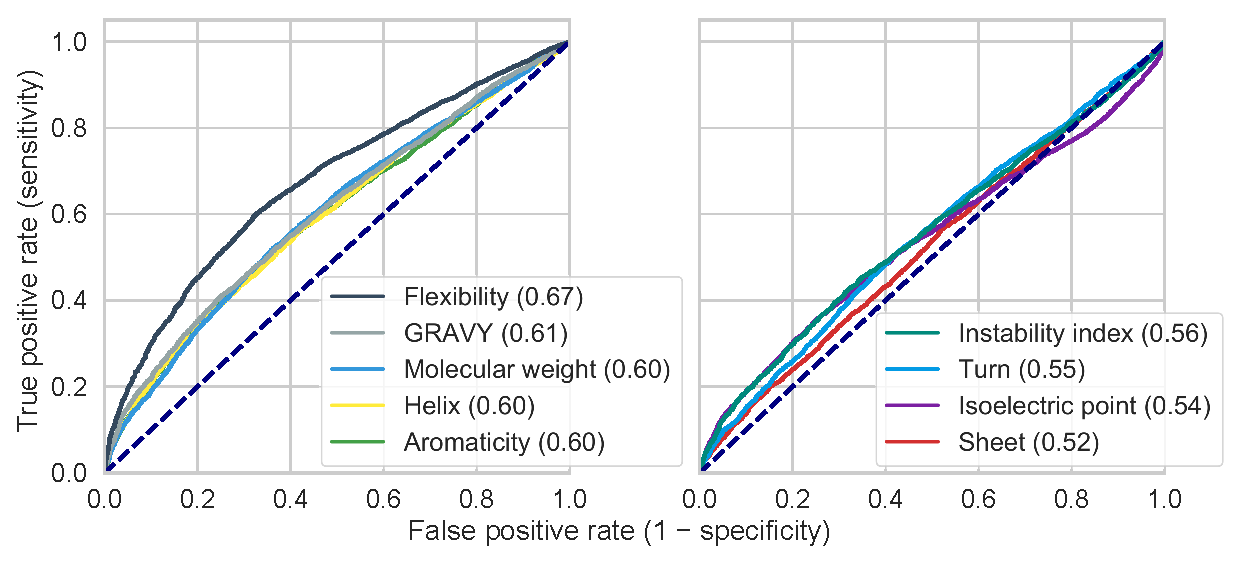
\includegraphics[width=1\textwidth]{chapters/Solubility/Figures/fig1.eps}}
\caption[Global structural flexibility outperforms other standard protein sequence properties in protein solubility prediction.]{{\bf Global structural flexibility outperforms other standard protein sequence properties in protein solubility prediction}. ROC analysis of the standard protein sequence features for predicting the solubility of 12,216 recombinant proteins expressed in {\it E. coli} (the PSI:Biology dataset). The ROC curves are shown in two separate panels for clarity. AUC scores (perfect = $1.00$, random = $0.50$) are shown in parentheses. Dashed lines denote the performance of random classifiers. See also Supplementary Fig \ref{fig:appendix_solubility_S2} and Table S2. AUC, Area Under the ROC Curve; GRAVY, Grand Average of Hydropathy; PSI:Biology, Protein Structure Initiative:Biology; ROC, Receiver Operating Characteristic.}\label{fig:solubility_01}
\end{figure}

\subsection{The Solubility-Weighted Index (SWI) is an improved predictor of solubility}
Protein structural flexibility, in particular, the flexibility of local regions, is often associated with function \citep{Craveur2015-wg}. The local flexibility of an amino acid residue $i$ can be written as:
\begin{equation}
\begin{split}
f_i = \frac{1}{5.25} \times [B_i + 0.8125(B_{i-1} + B_{i+1}) + \\ 0.625(B_{i-2} + B_{i+2}) + \\0.4375(B_{i-3} +B_{i+3}) +\\ 0.25(B_{i-4} + B_{i+4})]
\end{split}
\label{eqn:local_flexibility}\vspace*{-10pt}
\end{equation}
where $B_i$ denotes the normalised B-factor of amino acid residue $i$. These normalised B-factors were previously derived from the B-factors extracted from protein crystal structures \citep{Karplus1985-ea,Ragone1989-bx,vihinen1994accuracy,Smith2003-gb} (see also Supplementary Notes). These normalised B-factors can be applied to any protein sequences without crystallographic data for flexibility prediction, for example as implemented in Biopython.

To predict global protein structural flexibility $F$ (as in Fig \ref{fig:solubility_01}), $F$ can be calculated as the sliding window average of normalised B-factors (i.e., the arithmetic mean of $f_i$) \citep{vihinen1994accuracy,Cock2009-jl}. 
\begin{equation}
    F = \langle f_i \rangle
    \label{eqn:global_flex}\vspace*{-10pt}
\end{equation}

Therefore, we can simplify Equation \ref{eqn:local_flexibility} by setting $f'_i = B_i$ like a zeroth order Markov model. The simplified global flexibility $F'$ is then the arithmetic mean of normalised B-factors (see Supplementary Notes \ref{section:appendix_solubility_supp_notes} for mathematical proof ).
\begin{equation}
    F' = \langle f'_i \rangle = \langle B_i \rangle
    \label{eqn:Markov_model}\vspace*{-5pt}
\end{equation}

We found a strong correlation between $F$ and $F'$ for the PSI:Biology dataset (Spearman’s rho = $0.98$, P-value below machine’s underflow level). Hence, the sliding window approach (Equation \ref{eqn:local_flexibility} and \ref{eqn:global_flex}) is not necessary for this purpose.



% The calculation of flexibility is usually performed by assigning a set of 20 normalised B-factors to a protein sequence and averaging the values by a sliding window approach (the B-factor is a measure of vibration of the $C_\alpha$ atom, see Supplementary Notes) \citep{Karplus1985-ea,Ragone1989-bx,vihinen1994accuracy,Smith2003-gb}. We reasoned that such sliding window approach can be approximated by a more straightforward arithmetic mean for calculating global structural flexibility (see Supplementary Notes). We determined the correlation between flexibility (Vihinen {\it et~al.}’s sliding window approach as implemented in Biopython) and solubility scores calculated as follows:
% %
% \begin{equation}
%     \frac{1}{L}\sum_{i=1}^L B_{i}
%     \label{eq:01}
% \end{equation}
% %
% where $B_i$ is the normalised B-factor of the amino acid residue at the position $i$, and $L$ is the sequence length. A strong correlation was obtained (Spearman’s rho = $0.98$, P-value below machine’s underflow level), suggesting that the sliding window approach is not necessary for our purpose.


We applied this arithmetic mean approach (i.e., sequence composition scoring) to the PSI:Biology dataset using four sets of previously published, normalised B-factors \citep{Bhaskaran1988-bn,Ragone1989-bx,vihinen1994accuracy,Smith2003-gb}. Among these sets of B-factors, sequence composition scoring using the most recently published set of normalised B-factors produced the highest AUC score (AUC = $0.66$; Supplementary Fig \ref{fig:appendix_solubility_S3}).

To improve the prediction accuracy of solubility, we iteratively refined the weights of amino acid residues using the Nelder-Mead optimisation algorithm \citep{Nelder1965-zb} (Fig \ref{fig:solubility_02}). Smith {\it et~al.}’s normalised B-factors were used as initial weights. To avoid testing and training on similar sequences, we generated 10 cross-validation sets with a maximised heterogeneity between these subsets (i.e. no similar sequences between subsets). We clustered all 12,216 PSI:Biology protein sequences by a $40\%$ similarity threshold using USEARCH to produce 5,050 clusters with remote between-cluster similarity (see Methods  and Supplementary Fig \ref{fig:appendix_solubility_S4}). The clusters were grouped into 10 cross-validation sets of approximately 1,200 sequences each. As about $12\%$ of clusters contain a mix of soluble and insoluble proteins, we avoided selecting a representative sequence for each cluster (Supplementary Fig \ref{fig:appendix_solubility_S4}C). Furthermore, to avoid overfitting due to sequence similarity and imbalanced classes, we performed 1,000 bootstrap resamplings for each cross-validation step (Fig \ref{fig:solubility_02}A) and Supplementary Fig \ref{fig:appendix_solubility_S5}). We calculated the solubility scores using the optimised weights and the AUC scores for each cross-validation step as shown Fig \ref{fig:solubility_02}A. Our training and test AUC scores were $0.72 \pm 0.00$ and $0.71 \pm 0.01$, respectively, showing a 7.5\% improvement over flexibility in solubility prediction (mean $\pm$ standard deviation; Fig \ref{fig:solubility_02}B and  Supplementary Table \ref{tab:appendix_sodope_S3}).

\begin{figure}[!hbtp]
\centerline{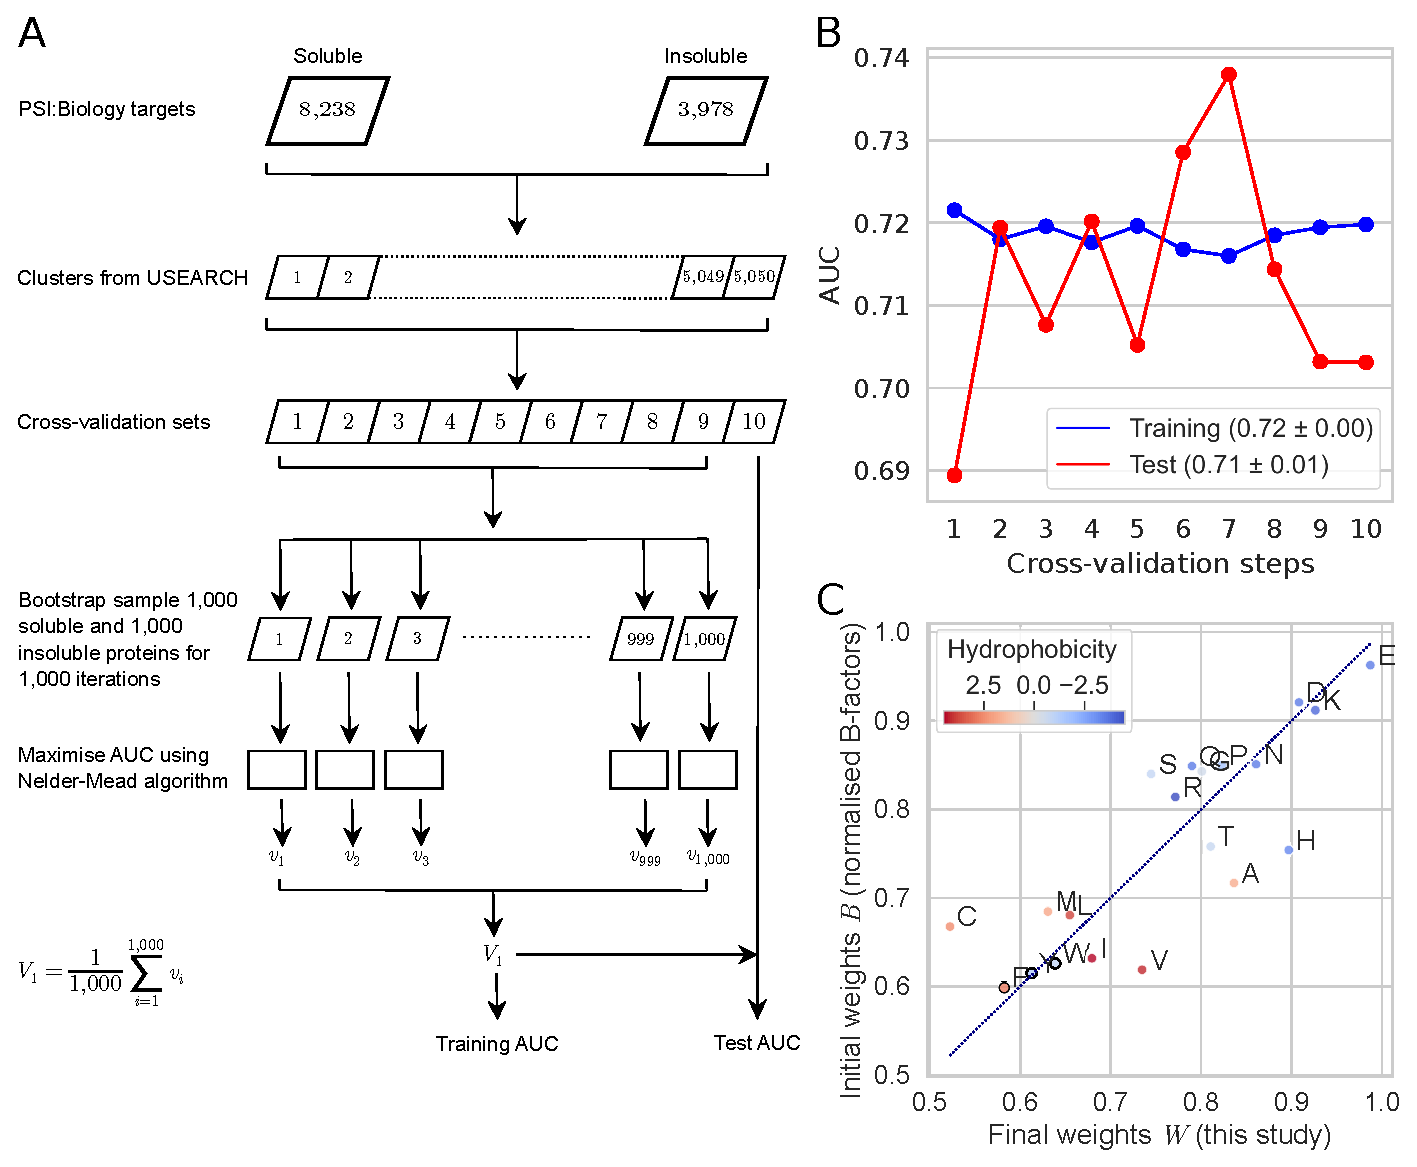
\includegraphics[width=1\textwidth]{chapters/Solubility/Figures/fig2.eps}}
\caption[Derivation of the Solubility-Weighted Index (SWI).]{{\bf Derivation of the Solubility-Weighted Index (SWI).} {\bf (A)} Flow chart shows an iterative refinement of the weights of amino acid residues for solubility prediction. Each cross-validation step used separate sequence similarity clusters for training and testing. Furthermore, bootstrapping was used to resample each training set, avoiding training and testing on similar sequences. The solubility scores of protein sequences were calculated using a sequence composition scoring approach. These scores were used to compute the AUC scores for training and test datasets. {\bf (B)} Training and test performance of solubility prediction using optimised weights for 20 amino acid residues in a 10-fold cross-validation (mean AUC $\pm$ standard deviation). Related data and figures are available as Supplementary Table \ref{tab:appendix_sodope_S3} and Supplementary Fig \ref{fig:appendix_solubility_S4} and \ref{fig:appendix_solubility_S5} . {\bf (C)} Comparison between the 20 initial and final weights for amino acid residues. The final weights $W = \langle V_i \rangle,\ 1\leq i\leq 10 $, were used to calculate the solubility score of a protein sequence (SWI) in the subsequent analyses. Filled circles, which represent amino acid residues, are colored by hydrophobicity \citep{Kyte1982-qn}. Solid black circles denote aromatic residues phenylalanine (F), tyrosine (Y), tryptophan (W). Dotted diagonal line represents no change in weight. See also Supplementary Table \ref{tab:appendix_sodope_S4}. AUC, Area Under the ROC Curve; ROC, Receiver Operating Characteristic.}\label{fig:solubility_02}
\end{figure}

\begin{figure}[!hbtp]
\centerline{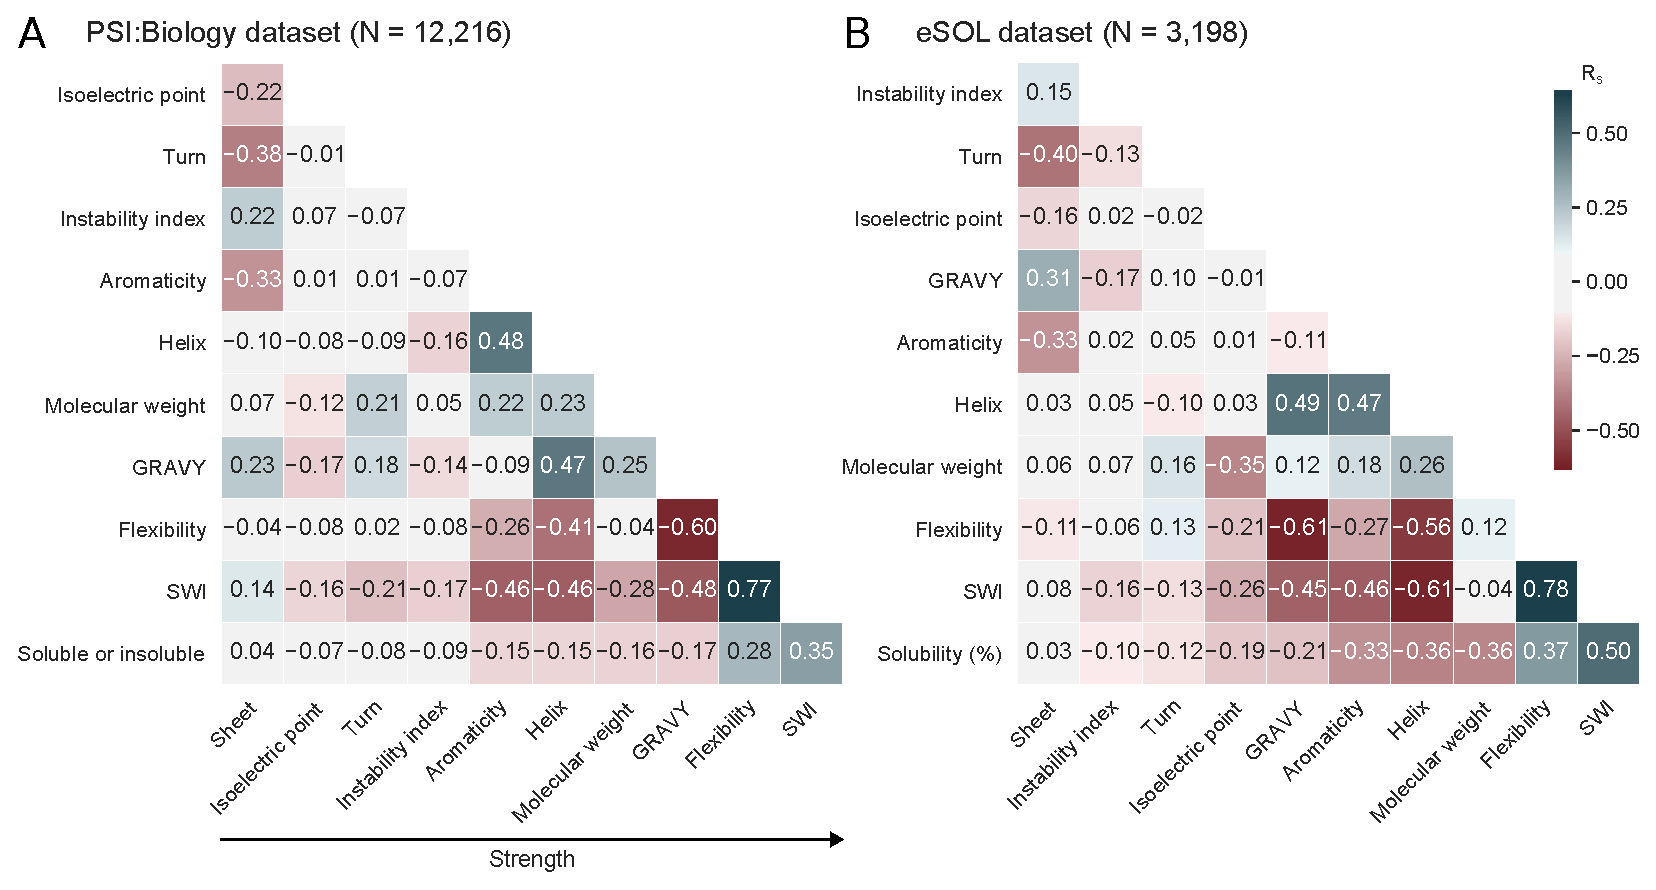
\includegraphics[width=1\textwidth]{chapters/Solubility/Figures/fig3.eps}}
\caption[SWI strongly correlates with protein solubility.]{{\bf SWI strongly correlates with protein solubility.} {\bf (A)} Correlation matrix plot of the solubility of recombinant proteins expressed in {\it E. coli} and their standard protein sequence properties and SWI. These recombinant proteins are the PSI:Biology targets (N = $12,216$) with a binary solubility status of 'Protein\_Soluble’ or 'Tested\_Not\_Soluble’. Related data is available as Supplementary Table \ref{tab:appendix_sodope_S5}. {\bf (B)} Correlation matrix plot of the solubility percentages of {\it E. coli} proteins and their standard protein sequence properties and SWI. The solubility percentages were previously determined using an {\it E. coli} cell-free system (eSOL, N = $3,198$). Related data is available as Supplementary Table \ref{tab:appendix_sodope_S6}. GRAVY, Grand Average of Hydropathy; PSI:Biology, Protein Structure Initiative:Biology; $R_s$, Spearman’s rho; SWI, Solubility-Weighted Index.
}\label{fig:solubility_03}
\end{figure}


The final weights were derived from the arithmetic means of the weights for individual amino acid residues obtained from cross-validation (Fig \ref{fig:solubility_02} and Supplementary Table \ref{tab:appendix_sodope_S4}). We observed over a $20\%$ change on the weights for cysteine (C) and histidine (H) residues (Fig \ref{fig:solubility_02}C and Supplementary Table \ref{tab:appendix_sodope_S4}). These results are in agreement with the contributions of cysteine and histidine residues as shown in Supplementary Fig \ref{fig:appendix_solubility_S2}B . We call the solubility score of a protein sequence calculated using the final weights the Solubility-Weighted Index (SWI):
\begin{equation}
    SWI = \langle W_i \rangle
    \label{eqn:swi}\vspace*{-10pt}
\end{equation}
where $W_i$ is the optimised weight of residue $i$.


To validate the cross-validation results, we used a dataset independent of the PSI:Biolgy known as eSOL \citep{Niwa2009-ye} (Supplementary Table \ref{tab:appendix_sodope_S1}). This dataset consists of the solubility percentages of \textit{E. coli} proteins determined using an \textit{E. coli} cell-free system (N = $3,198$). Our solubility scoring using the final weights showed a significant improvement in correlation with \textit{E. coli} protein solubility over the initial weights (Smith {\it et~al.}’s normalised B-factors) [Spearman’s rho of $0.50$ (P = $2.51 \times 10^{-205}$) versus $0.40$ (P = $4.57 \times 10^{-120}$)]. We repeated the correlation analysis by removing extra amino acid residues including His-tags from the eSOL sequences (MRGSHHHHHHTDPALRA and GLCGR at the N- and C-termini, respectively). This artificial dataset was created based on the assumption that His-tags have little effect on solubility. We observed a slight decrease in correlation for this artificial dataset (Spearman’s rho = $0.47$, P = $3.67 \times 10^{-176}$), which may be due to the effects of His-tags in solubility and/or the limitation(s) of our approach that may overfit to His-tag fusion proteins.

We performed Spearman’s correlation analysis for both the PSI:Biology and eSOL datasets. SWI shows the strongest correlation with solubility compared to the standard and 9,920 miscellaneous sequence properties (Fig \ref{fig:solubility_03} and Supplementary Fig \ref{fig:appendix_solubility_S2} , respectively; see also Supplementary Table \ref{tab:appendix_sodope_S2}, \ref{tab:appendix_sodope_S5}, \ref{tab:appendix_sodope_S6}). SWI strongly correlates with flexibility, suggesting that SWI is also a good proxy for global structural flexibility.


We asked whether protein solubility can be predicted by surface amino acid residues. To address this question, we examined a previously published dataset for the protein surface 'stickiness’ of $397$ \textit{E. coli} proteins \citep{Levy2012-ct}. This dataset has the annotation for surface residues based on previously solved protein crystal structures. We observed little correlation between the protein surface 'stickiness' and the solubility data from eSOL (Spearman’s rho = $0.05$, P = $0.34$, N = $348$; Supplementary Fig \ref{fig:appendix_solubility_S6}A ). Next, we evaluated if amino acid composition scoring using surface residues is sufficient, in which optimising only the weights of surface residues should achieve similar or better results than SWI. As above, we iteratively refined the weights of surface residues using the Nelder-Mead optimisation algorithm. The method was initialised with Smith {\it et~al.}’s normalised B-factors and a maximised correlation coefficient was the target. However, a low correlation was obtained upon convergence (Spearman’s rho = $0.18$, P = $7.20 \times 10^{-4}$; Supplementary Fig \ref{fig:appendix_solubility_S6}B ). In contrast, the SWI of the full-length sequences has a much stronger correlation with solubility (Spearman’s rho = $0.46$, P = $2.97 \times 10^{-19}$; Supplementary Fig \ref{fig:appendix_solubility_S6}C ). These results show that the full-length of sequences contributes to protein solubility, not just surface residues, suggesting that solubility is modulated by cotranslational folding \citep{Davis1999-ha,Natan2018-hv}.

To understand the properties of soluble and insoluble proteins, we determined the enrichment of amino acid residues in the PSI:Biology targets relative to the eSOL sequences (see Methods). We observed that the PSI:Biology targets are enriched in charged residues lysine (K), glutamate (E) and aspartate (D), and depleted in aromatic residues tryptophan (W), albeit to a lesser extend for insoluble proteins (Supplementary Fig \ref{fig:appendix_solubility_S7}A ). As expected, cysteine residues (C) are enriched in the PSI:Biology insoluble proteins, supporting previous findings that cysteine residues contribute to poor solubility in the \textit{E. coli} expression system \citep{Wilkinson1991-zp,Diaz2010-md}.

In addition, we compared the distributions of the SWI scores of soluble and insoluble proteins in the PSI:Biology and eSOL datasets. We included an analysis of random sequences to confirm whether SWI can distinguish between biological and random sequences. In general, the SWI scores of soluble proteins are higher than those of insoluble proteins (Supplementary Fig \ref{fig:appendix_solubility_S7}B ), and the SWI scores of true biological sequences are higher than those of random sequences, addressing our concern about the potential flaw of this position independent, sequence composition scoring approach.


\subsection{SWI outperforms many protein solubility prediction tools}
To confirm the usefulness of SWI in solubility prediction, we compared SWI with the existing tools CamSol v2.1 \citep{Sormanni2015-yr,Sormanni2017-lo}, ccSOL omics \citep{Agostini2014-te}, DeepSol v0.3 \citep{Khurana2018-xl}, PaRSnIP \citep{Rawi2018-xo}, Protein-Sol \citep{Hebditch2017-bg}, and the Wilkinson-Harrison model \citep{Wilkinson1991-zp,Davis1999-ha,Harrison2000-wm}. We did not include the specialised tools that model protein structural information such as surface geometry, surface charges and solvent accessibility because these tools require prior knowledge of protein tertiary structure. For example, Aggrescan3D and SOLart accept only PDB files that can be either downloaded from the Protein Data Bank or produced using a homology modeling program \citep{hou2020solart,Kuriata2019-ku}.

SWI outperforms other tools except for Protein-Sol in predicting \textit{E. coli} protein solubility (Fig \ref{fig:solubility_04} and Table~\ref{Tab:solubility_01}). The test AUC scores of SWI were also less variable than most other tools, suggesting that SWI is less prone to overfitting (Fig \ref{fig:solubility_02} and  \ref{fig:solubility_04}A). Our SWI C program is also the fastest solubility prediction algorithm (Fig \ref{fig:solubility_04}B, Table~\ref{Tab:solubility_01} and Supplementary Table \ref{tab:appendix_sodope_S6}).




%%%TABLE HERE
\begin{table*}%[]
% \processtable{Comparison of protein solubility prediction methods and software.\label{Tab:solubility_01}}
% {\resizebox{\textwidth}{!}{
\caption{Comparison of protein solubility prediction methods and software.}
\label{Tab:solubility_01}
{\resizebox{\textwidth}{!}{
\begin{tabular}{@{}llllll@{}}
\toprule
 &
  Approaches &
  Features &
  Wall time (s per sequence)\textsuperscript{a} &
  PSI:Biology (AUC)\textsuperscript{b} &
  eSOL {[}R\textsubscript{s} (P-value){]} \\ \midrule
SWI &
  \begin{tabular}[c]{@{}l@{}}Arithmetic mean (this study).\\
  Sequence composition scoring using a set of 20 values for amino \\ acid residues derived from Smith {\it et~al.}’s normalised B-factors. \\Trained and tested using the PSI:Biology dataset curated by\\ DNASU \citep{Seiler2014-on}. \\Available at \href{https://tisigner.com/sodope}{https://tisigner.com/sodope} and \\
  \href{https://github.com/Gardner-BinfLab/SoDoPE\_paper\_2020}{https://github.com/Gardner-BinfLab/SoDoPE\_paper\_2020}\end{tabular} &
  1 &
  {\bf 0.00  $\pm$ 0.00 }&
  {\bf 0.71  $\pm$ 0.01 } &
  0.50 (2.51 $\times$ 10\textsuperscript{$-$205}) \\ \midrule
Protein-Sol &
  \begin{tabular}[c]{@{}l@{}}Linear model \citep{Hebditch2017-bg}.\\  Trained and tested using eSOL dataset \citep{Niwa2009-ye}.\\  Available at \href{https://protein-sol.manchester.ac.uk/}{https://protein-sol.manchester.ac.uk/}\end{tabular} &
  10 &
  1.16  $\pm$ 0.75 &
  0.68 $\pm$ 0.02 &
  {\bf 0.54 (2.37 $\times$ 10\textsuperscript{$-$240})} \\\midrule
Flexibility &
  \begin{tabular}[c]{@{}l@{}}A sliding window of 9 amino acid residues using Vihinen {\it et~al.}’s \\normalised B-factors. \\Available at \href{https://github.com/biopython/biopython}{https://github.com/biopython/biopython}\end{tabular} &
  1 &
  0.38  $\pm$ 0.04 &
  0.67 $\pm$ 0.02 &
  0.37 (7.73 $\times$ 10\textsuperscript{$-$106}) \\\midrule
DeepSol S2 &
  {\begin{tabular}[c]{@{}l@{}}Neural network models \citep{Khurana2018-xl}\textsuperscript{c}.\\Trained and tested using a PSI:Biology dataset curated by\\ ccSOL omics \citep{Agostini2014-te}.\\ Available at \href{https://github.com/sameerkhurana10/DSOL\_rv0.2}{https://github.com/sameerkhurana10/DSOL\_rv0.2}\end{tabular}} &
  {57 (11 types)} &
  2069.77  $\pm$ 1613.63 &
  0.67 $\pm$ 0.02 &
  0.23 (5.82 $\times$ 10\textsuperscript{$-$41}) \\
DeepSol S3 &
   &
   &
  2075.93  $\pm$ 1613.80 &
  0.66 $\pm$ 0.02 &
  0.35 (7.48 $\times$ 10\textsuperscript{$-$91}) \\
DeepSol S1 &
   &
   &
  2081.93  $\pm$ 1612.71 &
  0.64 $\pm$ 0.03 &
  0.39 (9.52 $\times$ 10\textsuperscript{$-$116}) \\\midrule
CamSol intrinsic web server &
  \begin{tabular}[c]{@{}l@{}}Linear and logistic regression models (Sormanni {\it et~al} 2015, 2017).\\Trained and tested using previously published datasets \\\citep{Familia2015-mo}.\\Available at\\ \href{http://www-vendruscolo.ch.cam.ac.uk/camsolmethod.html}{http://www-vendruscolo.ch.cam.ac.uk/camsolmethod.html}\end{tabular} &
  4 &
  NA &
  0.66 $\pm$ 0.01 &
  0.44 (4.53 $\times$ 10\textsuperscript{$-$148}) \\\midrule
PaRSnIP &
  \begin{tabular}[c]{@{}l@{}}Gradient boosting machine model \citep{Rawi2018-xo}.\\Trained and tested using a PSI:Biology dataset curated by\\ ccSOL omics \citep{Agostini2014-te}.\\Available at \href{https://github.com/RedaRawi/PaRSnIP}{https://github.com/RedaRawi/PaRSnIP}\end{tabular} &
  8,477 (14 types) &
  2055.50  $\pm$ 1621.11 &
  0.61 $\pm$ 0.02 &
  0.29 (3.57 $\times$ 10\textsuperscript{$-$65}) \\\midrule
Wilkinson- Harrison model &
  \begin{tabular}[c]{@{}l@{}}Linear model using charge average and turn-forming \\residue fraction\\ \citep{Wilkinson1991-zp, Davis1999-ha, Harrison2000-wm}.\\Available at\\ \href{https://github.com/brunoV/bio-tools-solubility-wilkinson}{https://github.com/brunoV/bio-tools-solubility-wilkinson}\end{tabular} &
  2 &
  0.09  $\pm$ 0.00 &
  0.55 $\pm$ 0.03 &
  $-$0.06 (1.16 $\times$ 10\textsuperscript{$-$4}) \\\midrule
ccSOL omics web server &
  \begin{tabular}[c]{@{}l@{}}Support vector machine model \citep{Agostini2014-te}.\\Trained and tested using a PSI:Biology dataset curated in-house.\\Available at\\ \href{http://s.tartaglialab.com/new\_submission/ccsol\_omics\_file}{http://s.tartaglialab.com/new\_submission/ccsol\_omics\_file}\end{tabular} &
  5 &
  NA &
  0.51 $\pm$ 0.01 &
  $-$0.02 (0.18) \\ %\botrule
\end{tabular}}}{}
\small Boldface values are the best results.\\
\textsuperscript{a}The wall time was reported at the level of machine precision (mean seconds $\pm$ standard deviation). A total of 10 sequences were chosen from the PSI:Biology and eSOL datasets, related to Fig \ref{fig:solubility_04}B and Supplementary Table \ref{tab:appendix_sodope_S7} (see Methods).\\
\textsuperscript{b}For SWI, mean AUC $\pm$ standard deviation was calculated from a 10-fold cross-validation (see Methods). For other tools, no cross-validations were done as the AUC scores were calculated directly from the individual subsets used for cross-validation.\\
\textsuperscript{c}DeepSol reports solubility prediction as probability and binary classes. The probability of solubility was used to calculate AUC and Spearman’s correlation due to better results.\\
AUC, Area Under the ROC Curve; NA, not applicable; PDB, Protein Data Bank; PSI:Biology, Protein Structure Initiative:Biology; ROC, Receiver Operating Characteristic; R\textsubscript{s}, Spearman’s rho; SWI, Solubility-Weighted Index; s, seconds.
\end{table*}



\section{Discussion}
The profile of normalised B-factors along a protein sequence can be used to infer the flexibility and dynamics of the protein structure \citep{Karplus1985-ea,vihinen1994accuracy}. Protein structural flexibility has been associated with conformal variations, functions, thermal stability, ligand binding and disordered regions \citep{Vihinen1987-jo,Teague2003-vq,Radivojac2004-ff,Ma2005-cr,Schlessinger2005-ps,Yuan2005-gl,Yin2011-su}. However, the use of flexibility in solubility prediction has been overlooked although their relationship has previously been noted \citep{Tsumoto2003-qp}. In this study, we have shown that flexibility strongly correlates with solubility (Fig \ref{fig:solubility_03}). Based on the normalised B-factors used to compute flexibility, we have derived a new position and length independent weights to score the solubility of a given protein sequence  (i.e., sequence composition based score). We call this protein solubility score as SWI.



Upon further inspection, we observe some interesting properties in SWI. SWI anti-correlates with helix propensity, GRAVY, aromaticity and isoelectric point (Fig \ref{fig:solubility_02} and \ref{fig:solubility_03}), suggesting that SWI incorporates the key propensities affecting solubility. Amino acid residues with a lower aromaticity or hydrophilic are known to improve protein solubility \citep{Wilkinson1991-zp,Trevino2007-on,Niwa2009-ye,Kramer2012-wk,Warwicker2014-nh,han2019improve}. Consistent with previous studies, the charged residues aspartate (D), glutamate (E) and lysine (K) are associated with high solubility, whereas the aromatic residues phenylalanine (F), tryptophan (W) and tyrosine (Y) are associated with low solubility (Fig \ref{fig:solubility_02}C and Supplementary Fig \ref{fig:appendix_solubility_S7} ). Cysteine residue (C) has the lowest weight, probably because disulfide bonds couldn’t be properly formed in the \textit{E. coli} expression hosts \citep{Stewart1998-dn,Aslund1999-jl,Rosano2014-oq,jia2016high}. The weights are likely different if the solubility analysis was done using the reductase-deficient, \textit{E. coli} Origami host strains, or eukaryotic hosts.

Higher helix propensity has been reported to increase solubility \citep{Idicula-Thomas2005-qw,Huang2012-ft}. However, our analysis has shown that helical and turn propensities anti-correlate with solubility, whereas sheet propensity lacks correlation with solubility, suggesting that disordered regions may tend to be more soluble (Fig \ref{fig:solubility_03}). In accordance with these, SWI has stronger negative correlations with helix and turn propensities. Our findings also suggest that protein solubility can be largely explained by overall amino acid composition, not just the surface amino acid residues. This idea aligns with our understanding that protein solubility and folding are closely linked, and folding occurs cotranslationally, a complex process that is driven various intrinsic and extrinsic factors \citep{Wilkinson1991-zp,Davis1999-ha,Chiti2003-zk,Tartaglia2004-wm,Diaz2010-md,Natan2018-hv}. However, it is unclear why sheet propensity has little contribution to solubility as $\beta$-sheets have been shown to link closely with protein aggregation \citep{Idicula-Thomas2005-qw}.

\begin{figure}[!hbtp]
\centerline{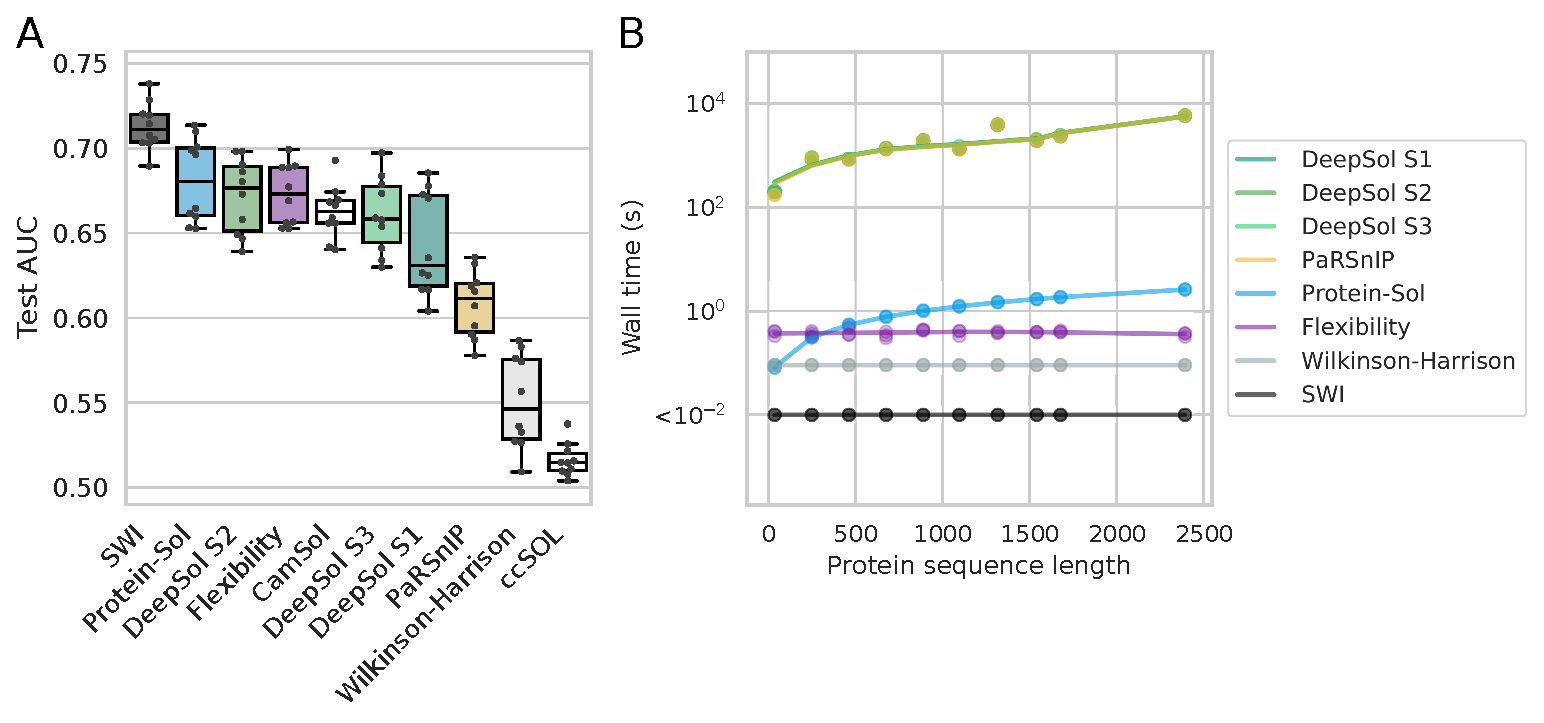
\includegraphics[width=1\textwidth]{chapters/Solubility/Figures/fig4.eps}}
\caption[SWI outperforms existing protein solubility prediction tools.]{{ \bf SWI outperforms existing protein solubility prediction tools. (A)} Prediction accuracy of solubility prediction tools using the above cross-validation sets (Fig \ref{fig:solubility_02}A). For SWI, the test AUC scores were calculated from a 10-fold cross-validation (i.e., a boxplot representation of Fig \ref{fig:solubility_02}B). For other tools, no cross-validations were done as the AUC scores were calculated directly from the individual subsets used for cross-validation. CamSol and ccSOL omics are only available as web servers (no fill colors). {\bf (B)} Wall time of protein solubility prediction tools per sequence (log scale). All command line tools were run three times using 10 sequences selected from the PSI:Biology and eSOL datasets. Related data is available as Supplementary Table \ref{tab:appendix_sodope_S7}. AUC, Area Under the ROC Curve; PSI:Biology, Protein Structure Initiative:Biology; ROC, Receiver Operating Characteristic; SWI, Solubility-Weighted Index; s, seconds.
}\label{fig:solubility_04}\vspace*{-10pt}
\end{figure}

We conclude that SWI is a well-balanced index that is derived from a simple sequence composition scoring method. To demonstrate the usefulness of SWI, we developed a web server called SoDoPE (Soluble Domain for Protein Expression; \href{https://tisigner.com/sodope}{https://tisigner.com/sodope}). SoDoPE calculates the probability of solubility of a user-selected region based on SWI, which can either be a full-length or a partial sequence (see Methods and Supplementary Table \ref{tab:appendix_sodope_S8}). This implementation is based on our observation that some protein domains tend to be more soluble than the others, and these soluble domains may enhance protein solubility as a whole. To demonstrate this point, we used SoDoPE to analyse three commercial monoclonal antibodies and the proteomes of the severe acute respiratory syndrome coronaviruses (SARS-CoV and SARS-CoV-2) \citep{Marra2003-zt,Wang2009-vj,Wu2020-oo} (Supplementary Fig \ref{fig:appendix_solubility_S8}  and \ref{fig:appendix_solubility_S9} ). SoDoPE also provides options for solubility prediction at the presence of solubility-enhancing tags. Similarly, these fusion tags may act as soluble ‘protein domains’ that can outweigh the aggregation propensity of insoluble proteins. However, some soluble fusion proteins may become insoluble after proteolytic cleavage of solubility tags \citep{Lebendiker2014-di}. In addition, SoDoPE is integrated with TIsigner, a web service for optimising protein expression \citep{Bhandari2021-wd}. This pipeline provides a holistic approach to improve the outcome of recombinant protein expression. \vspace*{-10pt}


% \begin{methods}
\section{Methods}

\subsection{Data}
We retrieved 12,216 PSI:Biology entries from the DNASU database \citep{Chen2004-cp,Acton2005-ng,Seiler2014-on}. These proteins were previously expressed in {\it E. coli} using pET21\_NESG or pET15 \_NESG expression vectors (N = $8,780$ and $3,436$, respectively). For validation, we used the solubility data of {\it E. coli} proteins from eSOL (N = $3,198$; \href{http://www.tanpaku.org/tp-esol/index.php?lang=en}{http://www.tanpaku.org/tp-esol/index.php?lang=en}) \citep{Niwa2009-ye}. See also Supplementary Fig \ref{fig:appendix_solubility_S1}  and Table S1A. 

In addition, we downloaded the 'stickiness’ data of $397$ \textit{E. coli} proteins to examine the effects of surface amino acid residues (\href{http://www.weizmann.ac.il/Structural\_Biology/faculty\_pages/ELevy/intDef/interface\_def.html}{http://www.weizmann.ac.il/Structural\\\_Biology/faculty\_pages/ELevy/intDef/interface\_def.html}) \citep{Levy2012-ct}.

\subsection{Protein sequence properties}
The standard protein sequence properties were calculated using the Bio.SeqUtils. ProtParam module of Biopython v1.73 \citep{Cock2009-jl}. All miscellaneous protein sequence properties were computed using the R package protr v1.6-2 \citep{Xiao2015-uw}. 

\subsection{Protein solubility prediction}
We used the standard and miscellaneous protein sequence properties to predict the solubility of the PSI:Biology and eSOL targets. For method comparison, we chose the protein solubility prediction tools that are scalable (Table~\ref{Tab:solubility_01}). Default configurations were used for running the command line tools.

To benchmark the wall time of solubility prediction tools, we selected 10 sequences that span a large range of lengths from the PSI:Biology and eSOL datasets (from 36 to 2,389 residues). All the tools were run and timed using a single process without using GPUs on a high performance computer [\verb|/usr/bin/time| \verb|-f| \verb|'%E'| \verb|<command>|]; CentOS Linux 7 (Core) operating system, 72 cores in 2 $\times$ Broadwell nodes (E5-2695v4, 2.1 GHz, dual socket 18 cores per socket), 528 GiB memory]. Single sequence fasta files were used as input files.


\subsection{SWI}
To improve protein solubility prediction, we optimised Smith {\it et~al.}’s normalised B-factors using the PSI:Biology dataset (Fig \ref{fig:solubility_02}). To avoid including homologous sequences in the test and training sets, we clustered the PSI:Biology targets using USEARCH v11.0.667, 32-bit \citep{Edgar2010-fc}. His-tag sequences were removed from all sequences before clustering to avoid false cluster inclusions. We obtained 5,050 clusters using the parameters: \verb|-cluster_fast| \verb|<input_file>| \verb|-id 0.4 -msaout| \verb|<output_file>| \verb|-threads 4|. These clusters were grouped into 10 subsets with approximately 1,200 sequences per subset manually. The subsequent steps were carried out using sequences with His-tags. 

We iteratively refined the weights of amino acid residues for solubility scoring using a 10-fold cross-validation, in which a maximised AUC was the target (Fig \ref{fig:solubility_02}A). Since AUC is non-differentiable, we used the Nelder-Mead optimisation method (implemented in SciPy v1.2.0), which is a derivative-free, heuristic, simplex-based optimisation \citep{Nelder1965-zb,Oliphant2007-za,Millman2011-tt}. For each step in cross-validation, we used bootstrap resamplings containing 1,000 soluble and 1,000 insoluble proteins. Optimisation was carried out for each sample, giving 1,000 sets of weights. The arithmetic mean of these weights was used to determine the training and test AUC for the cross-validation step. 


\subsection{Bit score}
To examine the enrichment of amino acid residues in soluble and insoluble proteins, we compute the bit scores for each residue in the PSI:Biology soluble and insoluble groups (Supplementary Fig \ref{fig:appendix_solubility_S7}A). The count of each residue (x) in each group was normalised by the total number of residues in that group. We used the normalised count of amino acid residues using the eSOL \textit{E. coli} sequences as the background. The bit score of residue $x$ for soluble or insoluble group is then given by the following equation:
%
\begin{equation}
    bit\ score (x_i) = log_2 \frac{f_i(x)}{f_{eSOL}(x)}, i =[soluble, insoluble]
    \label{eq:03}
\end{equation}
%
where $f_i(x)$ is the normalised count of residue $x$ in the PSI:Biology soluble or insoluble group and $f_{eSOL}(x)$  is the normalised count in the eSOL sequences.

For a control, random protein sequences were generated with incremental lengths, starting from a length of 50 residues to 6,000 residues with a step size of 50 residues. A hundred random sequences were generated for each length, giving a total of 12,000 unique random sequences.

\subsection{The SoDoPE web server}
To estimate the probability of solubility using SWI, we fitted the following logistic regression to the PSI:Biology dataset:
%
\begin{equation}
    probability\ of\ solubility = \frac{1}{1 + exp(-(ax + b))}
    \label{eq:04}
\end{equation}
%
where, $x$ is the SWI of a given protein sequence, $a = 81.05812$ and  $b = -62.7775$. The P-value of log-likelihood ratio test was below machine’s underflow level. Equation \ref{eq:04} can be used to predict the solubility of a protein sequence given that the protein is successfully expressed in \textit{E. coli} (Supplementary Table \ref{tab:appendix_sodope_S8}).

On this basis, we developed a solubility prediction web service called SoDoPE (Soluble Domain for Protein Expression). Our web server accepts either a nucleotide or amino acid sequence. Upon sequence submission, a query is sent to the HMMER web server to annotate protein domains (\href{https://www.ebi.ac.uk/Tools/hmmer/}{https://www.ebi.ac.uk/\\Tools/hmmer/}) \citep{Potter2018-ox}. Once the protein domains are identified, users can choose a domain or any custom region (including full-length sequence) to examine the probability of solubility, flexibility and GRAVY. This functionality enables protein biochemists to plan their experiments and opt for the domains or regions with high probability of solubility. Furthermore, we implemented a simulated annealing algorithm that maximised the probability of solubility for a given region by generating a list of regions with extended boundaries. Users can also predict the improvement in solubility by selecting a commonly used solubility tag or a custom tag.

We linked SoDoPE with TIsigner, which is our existing web server for optimising the accessibility of translation initiation site \citep{Bhandari2021-wd}. This pipeline allows users to predict and optimise both protein expression and solubility for a gene of interest. The SoDoPE web server is freely available at \href{https://tisigner.com/sodope}{https://tisigner.com/sodope}.

\subsection{Statistical analysis}
Data analysis was done using Pandas v0.25.3 \citep{McKinney2010-rg}, scikit-learn v0.20.2 \citep{Pedregosa2011-cd}, numpy v1.16.2 \citep{Van_der_Walt2011-hv} and statsmodel v0.10.1 \citep{Seabold2010-qk}. Plots were generated using Matplotlib v3.0.2 \citep{Caswell2018-pc} and Seaborn v0.9.0 \citep{Waskom2014-ar}. 


\subsection{Code and data availability}
Jupyter notebook of our analysis can be found at \href{https://github.com/Gardner-BinfLab/SoDoPE\_paper\_2020}{https://github.com/Gardner-BinfLab/SoDoPE\_paper\_2020}. The source code for our solubility prediction server (SoDoPE) can be found at \href{https://github.com/Gardner-BinfLab/TISIGNER-ReactJS}{https://github.com/Gardner-BinfLab/TISIGNER-ReactJS}.

% \end{methods}


% \section{Acknowledgements}
% We thank New Zealand eScience Infrastructure for providing a high performance computing platform. We are grateful to Harry Biggs for proofreading our manuscript and providing feedback for the web server. \vspace*{-12pt}


% \section{Funding}
% This work was supported by the Ministry of Business, Innovation and Employment, New Zealand (MBIE grant: UOOX1709).\vspace*{-12pt}

\chapter{Razor: annotation of signal peptides from toxins}
Dr Chun Shen Lim conceived the study. I performed all the data analysis and developed Razor (both the command line \href{https://github.com/Gardner-BinfLab/Razor}{https://github.com/Gardner-BinfLab/Razor} and the web server \href{https://tisigner.com/razor}{https://tisigner.com/razor}). I drafted the manuscript \cite{Bhandari2020-oj}. Dr Lim and Associate Professor Paul Gardner supervised the study. 

\section{Abstract}
Signal peptides are responsible for protein transport and secretion and are ubiquitous to all forms of life. The annotation of signal peptides is important for understanding protein translocation and toxin secretion and evolution. Here we explore the features of these signal sequences from eukaryotic proteins. Strikingly, we find that the signal peptides from secretory toxins share universal features across kingdoms, supporting the idea of horizontal gene transfer or convergence of toxin genes across kingdoms as shown by previous studies. We leverage these features to build Razor, a simple yet powerful tool specialised in identifying signal peptides from toxins using the first 23 N-terminal residues. We demonstrate the usability of Razor by analysing all the sequences reviewed by UniProt. Indeed, Razor is able to identify toxins using their N-terminal sequences only. Interestingly, we also discover that many defensive proteins across kingdoms harbour a toxin-like signal peptide; some of these defensive proteins have been shown to emerge through convergent evolution, e.g. defensin and defensin-like protein families, and phospholipase families. In sum, Razor uses an approach independent of homology search to identify novel and known toxin classes across species using N-terminal residues. Razor is available as a web application (https://tisigner.com/razor) and a command-line tool (https://github.com/Gardner-BinfLab/Razor).



\section{Introduction}
Secretory proteins are translocated in the secretory pathway with the assistance of a short peptide extension at the N-terminus. This special targeting peptide is known as the Signal Peptide (SP) \cite{Von_Heijne1990-sb}. Secretory pathways and their corresponding SPs have evolved across organisms to carry out different functions \cite{Hegde2006-od,Owji2018-hg}. Despite being ubiquitous across all domains of life, SPs do not share a consensus. Nevertheless, a SP usually consists of three regions: a positively charged domain (N-region), a hydrophobic core (H-region), followed by a polar but electrically neutral domain (C-region) containing a cleavage site \cite{Von_Heijne1985-qv,Von_Heijne1990-sb,Nielsen1998-dy}. Apart from translocating proteins, SPs are also responsible for several other roles, such as in regulatory functions, antigen presentation, and some human diseases \cite{Borrego1998-la,Datta2007-av,Owji2018-hg}.

An important group of secretory proteins is toxins, whose precursors almost always contain SPs \cite{Fry2009-iu}. Toxins have evolved in all domains of life primarily as a defense mechanism or for predation \cite{Casewell2013-pe}. Furthermore, several organisms in the animal kingdom have evolved to create venoms, which consist of a complex mixture of different types of toxins, usually with a specialised apparatus to facilitate their delivery. Such adaptations may have evolved through convergence or duplication and neofunctionalisation \cite{Casewell2020-qg}. However, a recent study found that at least five toxin gene families were horizontally transferred from bacteria and fungi to centipedes \cite{Undheim2021-eg}, suggesting common features exist in these gene families. Besides, the pharmacological actions of toxins on living cells are often employed to develop anti-toxins, novel drugs, and pathogen-resistant transgenic crops \cite{King2011-vf,Estrada2007-ij,Bidondo2019-zf,Samy2017-yi,Li2018-sr}. Hence, annotating SPs is essential in the functional and structural studies of proteins in fundamental research, commercial, and pharmaceutical industries. In addition, understanding the presence or absence of SPs in the genes of interest is critical for choosing the appropriate recombinant protein expression and purification systems, as the intracellular accumulation of secretory proteins and toxins may be toxic to the host cells. Indeed, the ability of SPs to translocate proteins has been utilised in recombinant protein expression systems for high quality and quantity results \cite{Futatsumori-Sugai2010-iu,Cho2019-dq,Karyolaimos2019-ip,Peng2019-xc}.

Despite the immense use cases of toxins, there are very few tools to predict them, such as ClanTox, ToxinPred, TOXIFY, and ToxClassifier, some being specialised such as SpiderP for spider toxins \cite{Naamati2010-vc,Gupta2013-fw,Wong2013-qh,Gacesa2016-fl,Cole2019-bp}. Moreover, these methods are based on the properties of the mature peptides (or the propeptides), rather than the SPs. To address these issues, we first examined the features of SPs from eukaryotic proteins and toxins. We then exploited those features to build Razor, a new tool for annotating SPs. We have optimised the command-line version of Razor for high-throughput analysis and used it to predict new SPs by scanning all the sequences reviewed by UniProt \cite{UniProt_Consortium2019-ch}. We were able to predict novel toxins and defensive proteins using only the first 23 N-terminal residues, as evidenced by the protein family annotations.

\section{Results}
\subsection{Toxin SPs have distinct sequence properties}
We investigated the sequence composition of SPs by first aligning the sequences from the N-terminal residue or by centering at the cleavage sites, followed by computing bit scores for each residue (Fig  \ref{fig:razor_02}). These approaches provide sufficient leverage to enumerate the tripartite domains of SPs (N-, H-, and C-domains). In general, hydrophobic residues are enriched towards the N-termini (H-region), which are characteristic features of SPs \cite{Von_Heijne1990-sb} (Supplementary Fig \ref{fig:appendix_razor_S1}). Strikingly, the SPs of toxins show a strong abundance of isoleucine (I) and lack leucine (L) and alanine (A) residues in contrast to other eukaryotic SPs (Fig \ref{fig:razor_02}). This is supported by an amino acid composition analysis of the N-terminal subsequences (Supplementary Fig \ref{fig:appendix_razor_S2}). We also analysed other features of these N-terminal subsequences, including GRAVY, structural flexibility, helix, sheet and turn propensities, instability index, aromaticity, isoelectric point, and SWI. Interestingly, isoelectric point appears as a prominent feature of toxin SPs (Supplementary Fig \ref{fig:appendix_razor_S3}).


The cleavage sites mark the end of SPs and the beginning of the mature region (or the propeptide), which is a unique feature of SPs (Fig \ref{fig:razor_02}). By aligning the sequences at the cleavage sites, we observed a clear emergence of (−3,−1) rule preceding the cleavage sites, i.e. a distinctive presence of small and charged residues such as alanine (A) and valine (V) \cite{Von_Heijne1983-hr}.

\begin{figure}[!hbtp]
\centerline{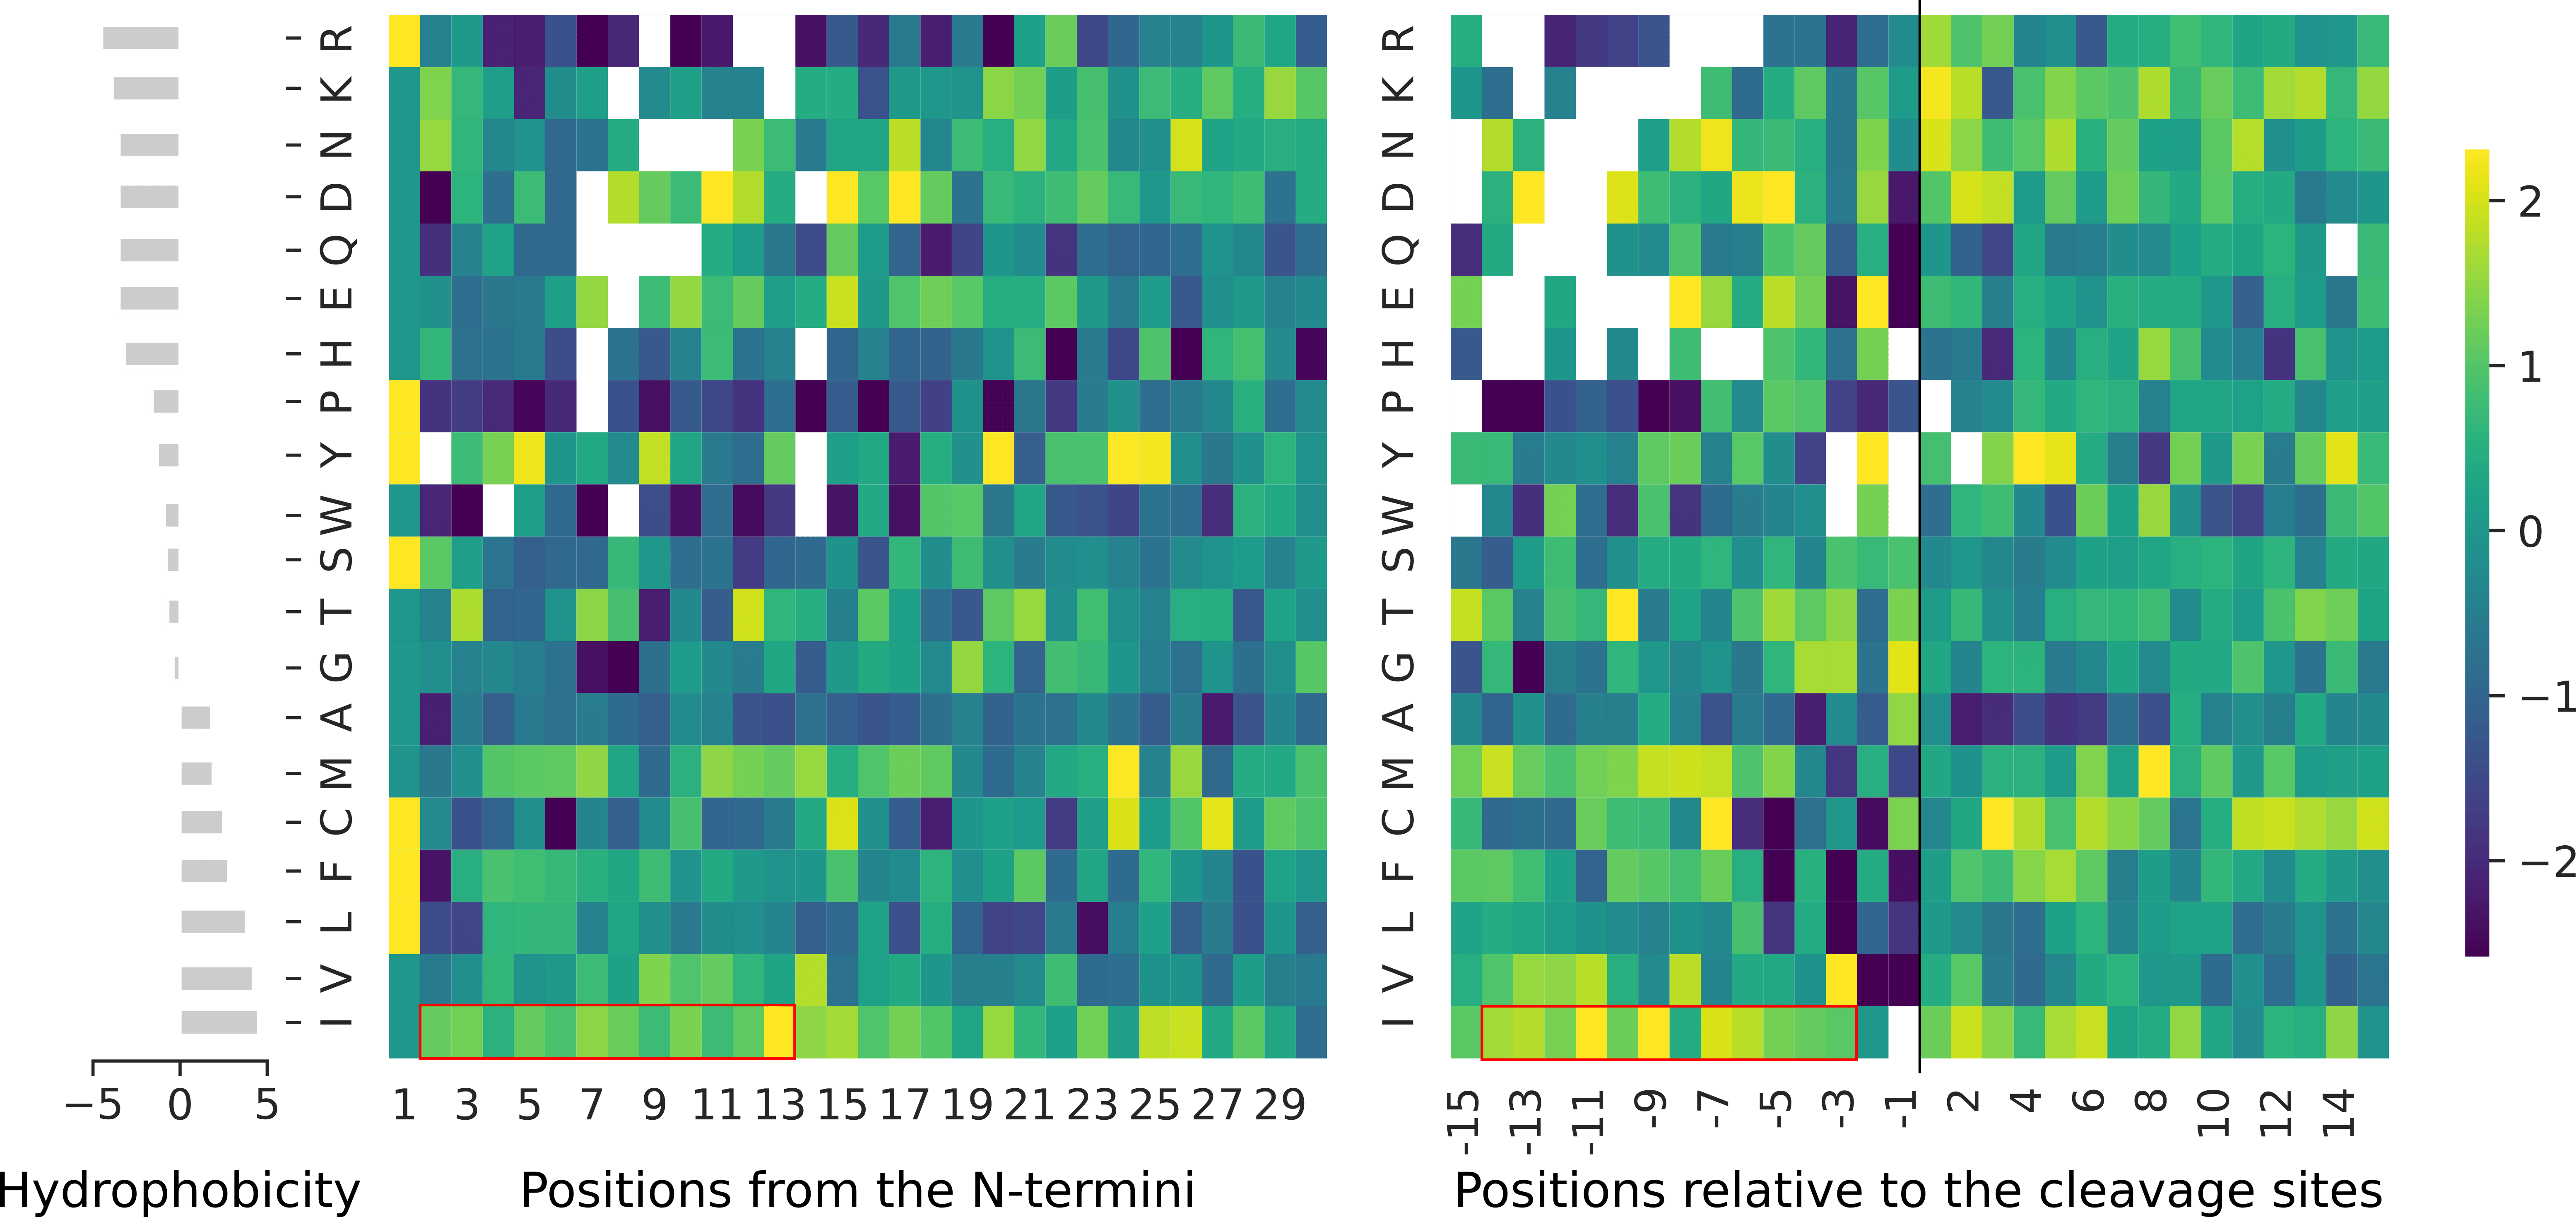
\includegraphics[width=1\textwidth]{chapters/Signal_Peptide/Figures/fig1_bitscore_heatmap_toxin.png}}
\caption[The Signal Peptides (SPs) from toxins are enriched with isoleucine residues in contrast to other eukaryotic SPs.]{\textbf{The Signal Peptides (SPs) from toxins are enriched with isoleucine residues in contrast to other eukaryotic SPs.} The bar plot shows Kyte and Doolittle’s hydrophobicity scale. The heatmaps show the enrichment of residues in bit scores by aligning SPs from the N-termini (left) and at the cleavage sites (right, black vertical line). The unfilled, red rectangles indicate the enrichment of isoleucine residues (I). The white spaces correspond to the absence of residues at certain positions due to limited sample size (261 toxin SPs and 1,738 non-toxin SPs that have been experimentally validated).
}\label{fig:razor_02}
\end{figure}



\subsection{Razor accurately predicts toxin SPs}
By taking these important features into account, we built SP classifiers to annotate eukaryotic and toxin SPs using random forest (Fig \ref{fig:razor_01}). Only SPs with experimental evidence were used for training. We compared these classifiers using an independent test set, where, the MCC, and the cleavage site precision and recall of Razor for eukaryotic SP prediction were 0.405, 0.136, 0.596, respectively (SPs vs non-SPs, see Supplementary Fig \ref{fig:appendix_razor_S4}, Table S3 and S4). More importantly, Razor outperforms state-of-the-art in toxin SP prediction, achieving an MCC score of 0.611, and the cleavage site precision and recall of 0.355 and 0.831, respectively (toxin SPs vs non-SPs, see (Fig \ref{fig:razor_03}), and Supplementary Table \ref{tab:razor_benchmark_independent_test_set_toxin_mcc} and \ref{tab:razor_benchmark_independent_test_set_toxin_precision_recall}).


\begin{figure}[!hbtp]
\centerline{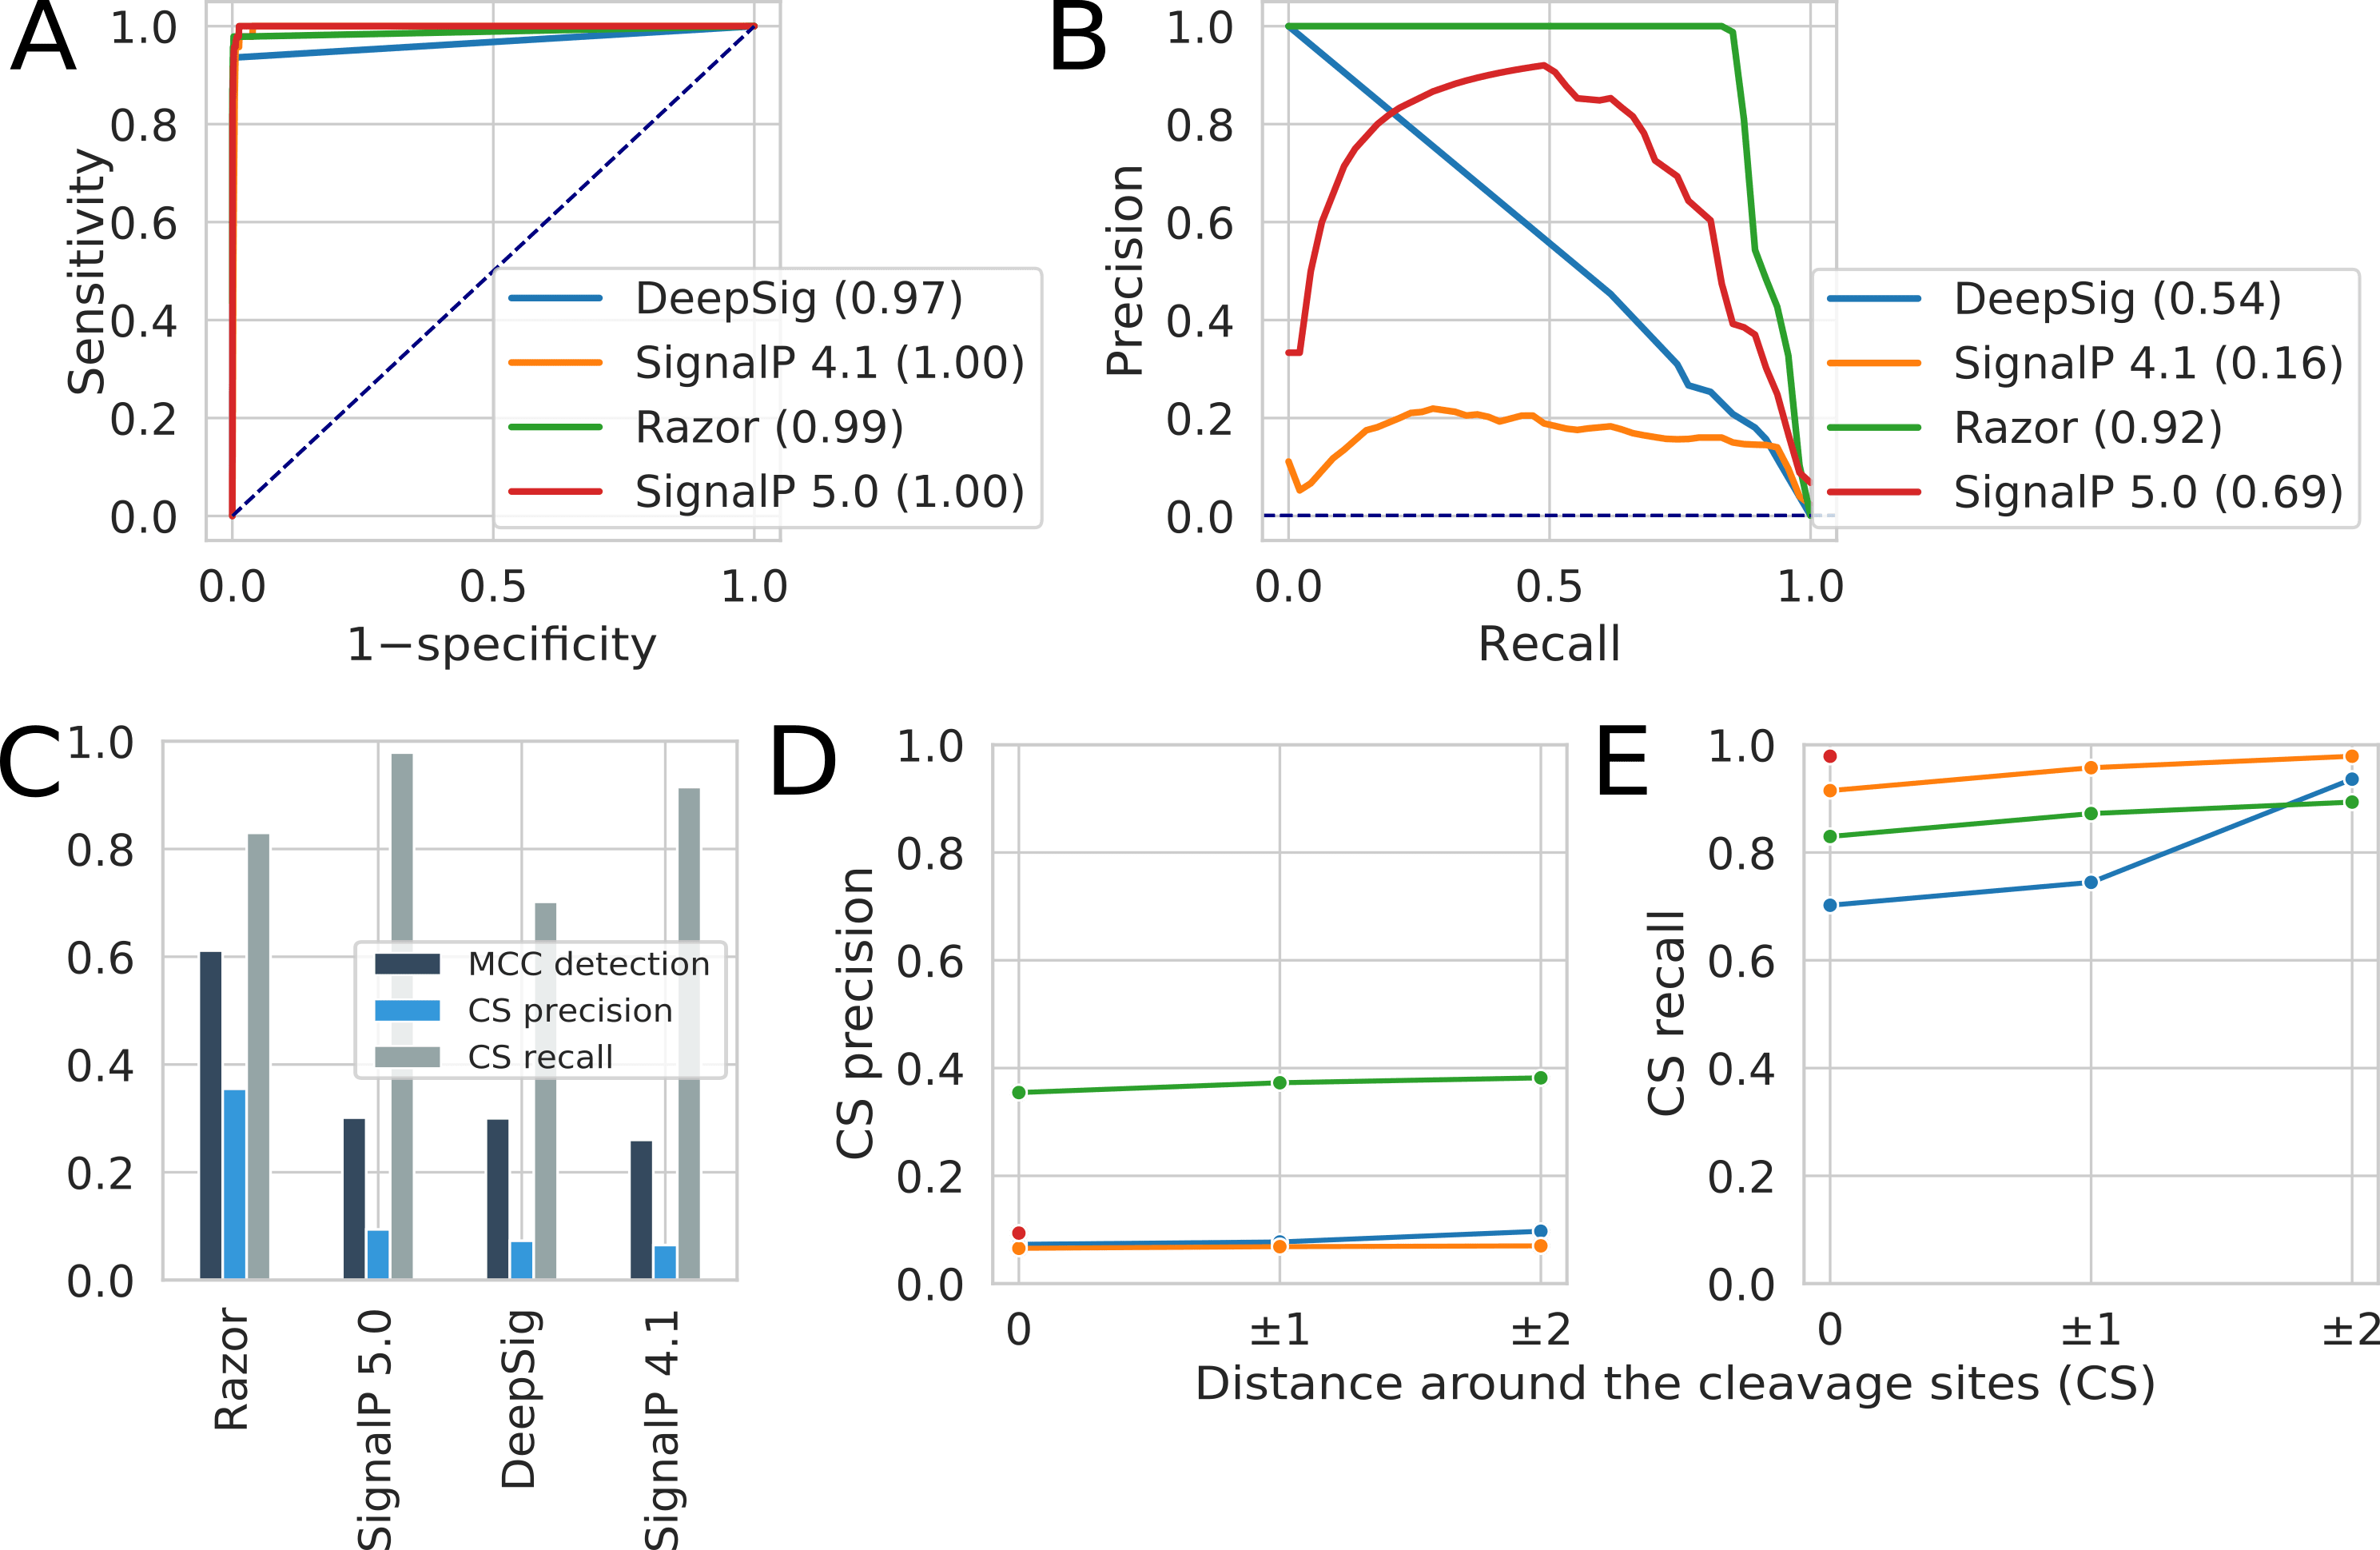
\includegraphics[width=1\textwidth]{chapters/Signal_Peptide/Figures/fig3_new_benchmarking_cleavage_sites_with_toxin.png}}
\caption[Razor outperforms other tools in predicting toxin SPs. ]{\textbf{Razor outperforms other tools in predicting toxin SPs. } Benchmarks were carried out using an independent test set (47 experimentally validated toxin SPs and 52,055 non-SPs). \textbf{(A)} Receiver operating characteristic curves \textbf{(B)}  and precision recall curves \textbf{(C)}  of the SP prediction tools. Areas under the curves are shown in parentheses. The dotted lines show the performance of a random classifier. \textbf{(C)}  Matthew’s Correlation Coefficients (MCC) of the SP prediction tools. The cleavage site (CS) precisions \textbf{(D)}  and recalls \textbf{(E)}  of windows surrounding the cleavage sites are shown. Data are available in Supplementary Tables \ref{tab:razor_benchmark_independent_test_set_toxin_mcc} and \ref{tab:razor_benchmark_independent_test_set_toxin_precision_recall}.
}\label{fig:razor_03}
\end{figure}


\subsection{Defensive proteins harbour a toxin-like SP}
The training set for the toxin SP classifier was mainly composed of the SPs from animal toxins, e.g. snake three-finger toxins, scorpion toxins, and phospholipase A2, and plant toxins, e.g. ribosome-inactivating proteins (Fig \ref{fig:razor_04}A). To further assess our new toxin SP classifier, we scanned the reviewed sequences from UniProt (N=561,776). A total of 910 sequences were predicted positive from all SP detection models. 

\begin{figure}[!hbtp]
\centerline{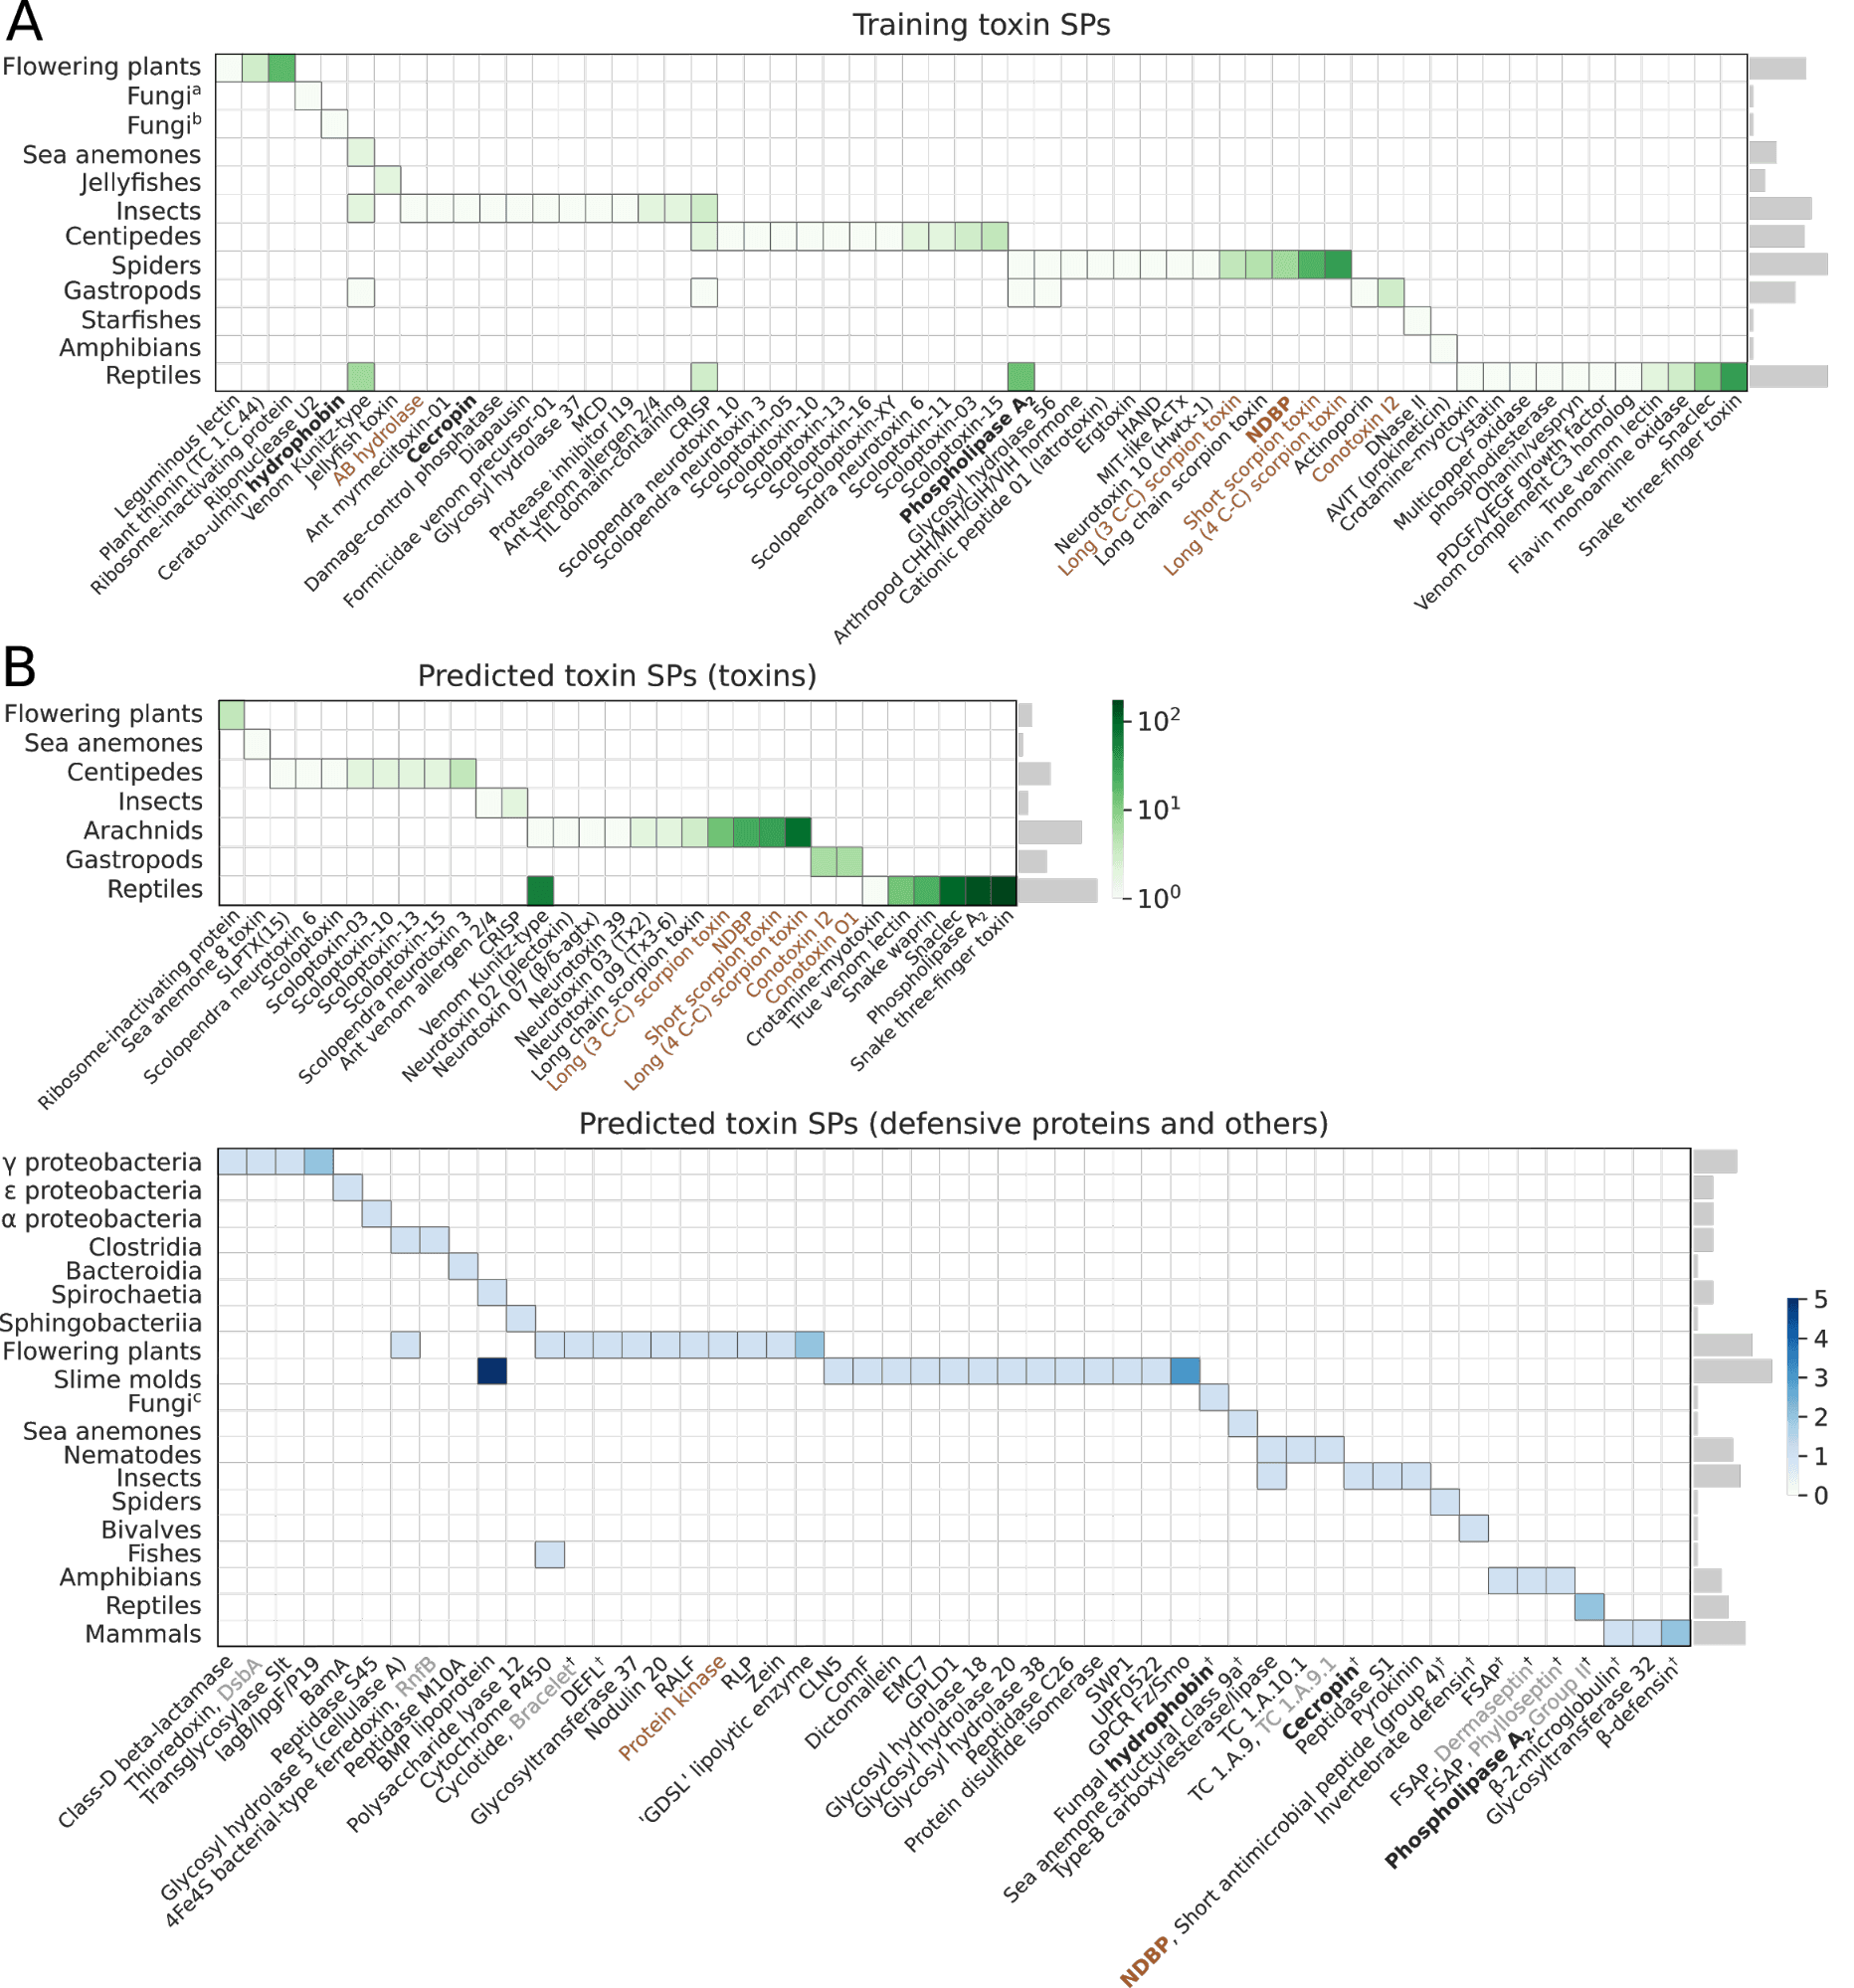
\includegraphics[width=0.85\textwidth]{chapters/Signal_Peptide/Figures/fig4_tox.png}}
\caption[Razor identifies SPs from toxins along with several classes of defensive proteins.]{\textbf{Razor identifies SPs from toxins along with several classes of defensive proteins.} The reviewed sequences from UniProt were examined (N=561,776). \textbf{(A)} Heatmap shows the abundance of protein families in the training toxin sequences with SPs by taxa. A total of 237 of 261 training toxins had protein family annotations. \textbf{(B)} Heatmaps show the abundance of protein families in the sequences predicted to harbour toxin SPs. A total of 753 of 759 toxins predicted to harbour toxin SPs had protein family annotations (top). A total of 110 other types of proteins were predicted to harbour toxin SP, in which 76 of them had protein family annotations (bottom). The scale bars indicate the frequencies of protein families. Those protein families that have defensive properties are marked with $\dagger$ (bottom). Protein families that are in common between the training and predicted toxin SP sequences are bolded (bottom panel). Protein subfamily, family and superfamily are shown in grey, black and brown, respectively. Fungi\textsuperscript{a}, Eurotiomycetes; Fungi\textsuperscript{b}, Sordariomycetes; Fungi\textsuperscript{c}, Agaricomycetes; CLN5, Ceroid-Lipofuscinosis Neuronal protein; ComF, Competence protein F; CRISP, Cysteine RIch Secretory Protein; DEFL, DEFensin Like; EMC7, ER membrane protein complex subunit 7; FSAP, Frog Skin Antimicrobial Peptide; GPLD1, Glycosyl-phosphatidylinositol-specific phospholipase D; HAND, Helical Arthropod-Neuropeptide-Derived; RALF, Rapid ALkalinization Factor; RLP, Receptor Like Protein; SLPTX, Scoloptoxin; UPF, Uncharacterised Protein Family.
}\label{fig:razor_04}
\end{figure}

%\begin{figure}
%\captionsetup{labelformat=empty}
%\caption[]{
% Fungi\textsuperscript{a}, Eurotiomycetes; Fungi\textsuperscript{b}, Sordariomycetes; Fungi\textsuperscript{c}, Agaricomycetes; CLN5, Ceroid-Lipofuscinosis Neuronal protein; ComF, Competence protein F; CRISP, Cysteine RIch Secretory Protein; DEFL, DEFensin Like; EMC7, ER membrane protein complex subunit 7; FSAP, Frog Skin Antimicrobial Peptide; GPLD1, Glycosyl-phosphatidylinositol-specific phospholipase D; HAND, Helical Arthropod-Neuropeptide-Derived; RALF, Rapid ALkalinization Factor; RLP, Receptor Like Protein; SLPTX, Scoloptoxin; UPF, Uncharacterised Protein Family.
%}
%\end{figure}



In (Fig \ref{fig:razor_04}), we excluded potential false positive hits, i.e. computationally annotated transmembrane proteins by UniProt (N=33). The remaining sequences were divided into two groups based on the presence or absence of toxin annotation. From these probable toxin SPs, 759 sequences had annotations for toxins. They included protein families such as scorpion toxin, phospholipase A2 and ribosome-inactivating protein (Fig \ref{fig:razor_04}B). The remaining 110 sequences had no annotations for toxins. These sequences were clustered at an identity threshold of 70\%, which gave rise to 100 representative sequences. Interestingly, many of these proteins without toxin annotations have some defensive properties such as antibacterial peptides and cyclotides. Furthermore, other defensive proteins such as beta-defensin and defensin-like (DEFL) are the results of convergent evolution. For example, beta-defensin-like motifs are also found in toxins from lepidosauria (rattlesnakes and bearded dragons) and mammalia (platypus) \cite{Fry2009-iu,Fry2010-bs,Whittington2008-vm}. This suggests why their SPs show some remote similarity with toxin SPs.


\section{Discussion}
We have studied the features of SPs from eukaryotic proteins. While SPs share a common hydrophobic nature, we have found several differences between toxin SPs and other eukaryotic SPs in their residue compositions and consequently the sequence properties. We have used these features to develop Razor for annotating eukaryotic SPs, which have specialised functionalities in annotating toxin SPs. Razor outperforms other sophisticated methods in predicting toxin SPs. Using Razor, we were able to predict several classes of probable toxins, which are yet to be annotated (Fig \ref{fig:razor_04}). Our predicted results consist of toxins and defensive proteins from diverse species, which gives us an overview of the source of toxins.

Since toxins and defensive proteins occur naturally in organisms to attack and neutralise foreign invaders, many of our predicted results include proteins involved in innate immune response and signalling. Some of the frequently observed biological processes of these proteins were ‘killing of cells of other organism [GO:0031640]’, ‘defense response to fungus [GO:0050832]’, ‘defense response to bacterium [GO:0042742]’ and ‘innate immune response [GO:0045087]’ (Supplementary Fig \ref{fig:appendix_razor_S5} and \ref{fig:appendix_razor_S6}). Many toxins and defensive proteins are commercially important. For example, plant toxins such as defensin-like protein, animal toxins such as cecropin are used to develop disease-resistant transgenic crops \cite{Stotz2009-dj,Lacerda2014-ce,Wu2016-hf,Boccardo2019-hi,Ali2018-jt}. Similarly, the cytotoxic activity of phospholipase A2 on cancer cells makes it a promising candidate for cancer therapy \cite{Xiao2017-vm,Hiu2020-fr,Lomonte2012-ug}. 

Taken together, Razor uses an approach independent of homology search to identify known and novel toxin classes across species. Razor was able to identify previously unannotated SPs and a spectrum of toxins and defensive proteins simply using the first 23 N-terminal residues. This also suggests a possible evolutionary constraint on SPs driven by the specialisation of the toxin secretory systems (or convergent evolution), and supports the idea of horizontal gene transfer of several toxin gene classes \cite{Undheim2021-eg}. Therefore, accurate annotation of toxin SPs can enhance comparative genomics analysis and genome sequencing projects. Razor might also be useful in other research areas such as recombinant protein expression, toxicology, transgenics, and drug design.





\section{Methods}
\subsection{Datasets}
We retrieved the training dataset for the state-of-the-art SP prediction program SignalP 5.0, which is a curated set of the N-terminal sequences from all domains of life \cite{Almagro_Armenteros2019-vr}. To get the full sequences and annotations of eukaryotic proteins, we used UniProt’s ID mapping service \cite{UniProt_Consortium2019-ch} and obtained 17,264 fully annotated sequences, of which 2,609 sequences have been experimentally validated to harbour functional SPs. These sequences were used to build a generic, eukaryotic SP classifier. For feature analysis, we clustered these sequences (60 N-terminal residues) at an identity threshold of 70\% using CD-HIT v4.8.1 \cite{Fu2012-ng}. A single representative sequence was retained for each cluster to reduce sequence redundancy (Supplementary Table \ref{tab:razor_datasets}).

To build a classifier specialised for annotating toxin SPs, we manually curated a separate positive set using the dataset from the animal toxin annotation project \cite{Jungo2012-ja} and a subset from the above training set. Other SPs were assigned as a negative set. We then clustered the sequences as above and analysed the representative sequences (Supplementary Table \ref{tab:razor_datasets}). 

The SP classifiers were compared using an independent test set retrieved from UniProt on 16 February 2021. In particular, the eukaryotic SP classifier was evaluated using 241 SPs with experimental evidence and 52,055 non-SPs, whereas the toxin SP classifier was evaluated using a subset of this independent set (toxin SPs=47, non-SPs=52,055). We also scanned the reviewed sequences from UniProt (N=561,776, retrieved on 2 September 2020).

\subsection{Bit score}
The bit scores of the N-terminal residues were computed as:
%
\begin{equation}
    bit\ score (residue) = log_2 \frac{Normalised\ count\ of\ residue\ in\ positive\ set}{Normalised\ count\ of\ residue\ in\ negative\ set}
    % \label{eq:03}
\end{equation}
%
For eukaryotic proteins, the positive set and the background set were SPs and non-SPs, respectively. For toxins, the positive set and the background set were toxin SPs and non-toxin SPs, respectively.


\subsection{Protein sequence properties}
The standard protein sequence properties, implemented in BioPython, were calculated using the Bio.SeqUtils.ProtParam module v$1.73$ \cite{Cock2009-ym}. These features include GRand AVerage of hydropathicitY (GRAVY), Flexibility, Helix, Sheet and Turn propensities, Instability Index, Aromaticity, and Isoelectric Point. An additional feature included is the Solubility-Weighted Index (SWI; \cite{Bhandari2020-pz}.

\subsection{SP classifiers}
We built a random forest classifier based on several sequence features (GRAVY, flexibility, helix, and SWI), as well as the counts of residues (R, K, N, D, C, E, V, I, Y, F, W, L, Q, and P) of the first 30 N-terminal residues. The residues were chosen such that they maximised Matthew's correlation coefficient (MCC) in five-fold cross-validations. After the cross-validation step, we generated five random forest models, which are used for scoring the N-terminal of a given sequence. The scores from these classifiers are comparable to the S-score of SignalP 4.0 except that our scores are non-position-specific \cite{Petersen2011-ex}.

For the prediction of the cleavage site, we took a total of 30 residues such that the cleavage site is aligned in between positions 15 and 16 in order to capture the major differences in residue distribution around the cleavage site. We built a $20\times30$ matrix and populated it with the hydrophobicity scale \cite{Kyte1982-qn} as initial weights. We then used multi-objective simulated annealing \cite{Kirkpatrick1983-hh} at each position such that the new weights maximised the AUC and precision-recall curve based on the training set. The scoring of the cleavage site (C-score) is done using the random forest classifier trained on the aligned set encoded using the optimised weight matrix. Small limitation of our approach is that we are unable to detect the correct cleavage site if it is located before the 15th position. Yet, based on training data, this is rarely observed (N=13).

After detecting the cleavage site, the final score for classification (Y-score) is the geometric mean $Y = \sqrt{S \times C} $, where S is the S-score and C is the max of C-scores along the sequence. For the final classifier, we chose a threshold of Y-score that maximised the MCC after five-fold cross-validations (MCC=0.914) on the training set.

We then built models specialised in annotating the toxin SPs based on hydrophobicity, SWI, flexibility, and turn. These features were selected such that they maximised the MCC using five-fold cross-validations on the training set. The N-terminal length of 23 was found to generate the maximum median MCC score for the toxin SP classifier (MCC=0.741, see also Supplementary Table \ref{tab:razor_feature_selection}). Similar to the SP prediction models, the toxin SP classifiers consist of five models each.

\subsection{Performance measures}
We use MCC as a measure of performance to correctly identify eukaryotic SPs. We also use cleavage site precision $(CS_P=N_{corr}/N_P)$ and recall $(CS_R=N_{corr}/N)$, where $N_{corr}$ is the number of the correctly identified cleavage site, $N_P$ is the number of predicted SPs and $N$ is the number of SPs \cite{Almagro_Armenteros2019-vr,Savojardo2017-ux}.

\subsection{Tool}
We developed Razor for annotating SPs using the eukaryotic and toxin SP classifiers (Fig \ref{fig:razor_01}).


\begin{wrapfigure}{r}{0.5\textwidth}
  \begin{center}
    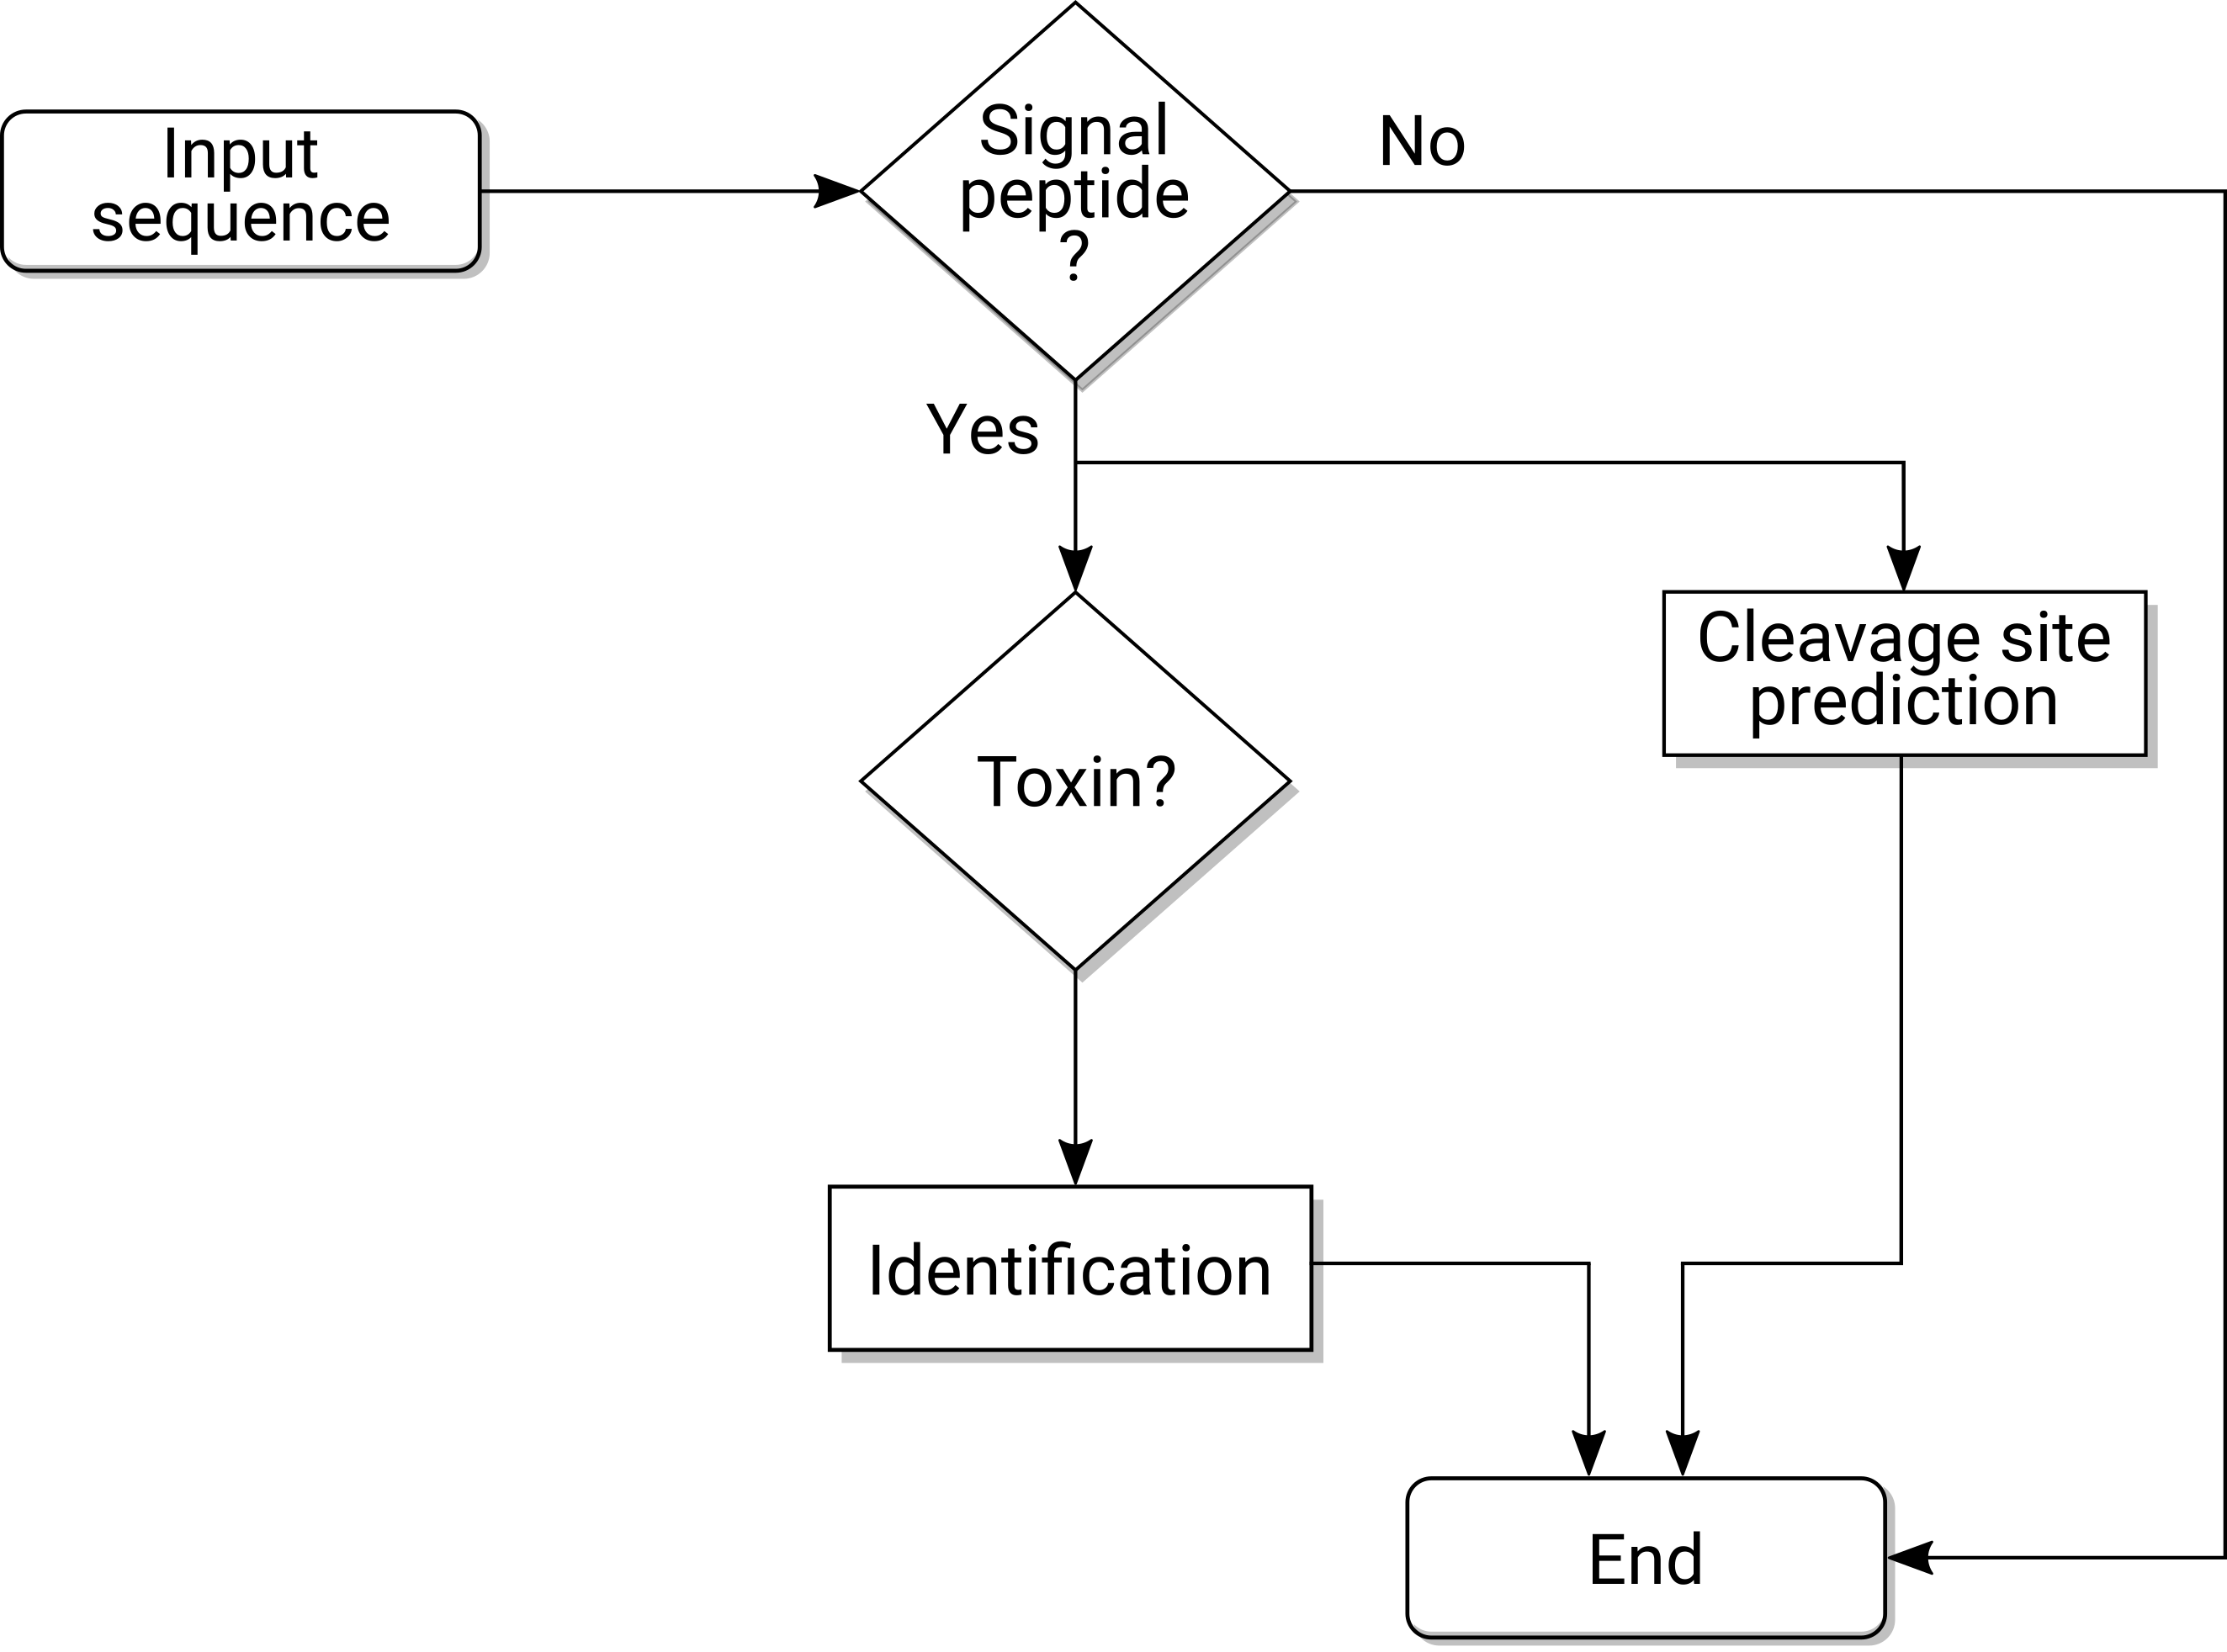
\includegraphics[width=0.45\textwidth]{chapters/Signal_Peptide/Figures/flowchart-fs8.png}
    \caption[Flow chart of toxin SP classification using Razor.]{Flow chart of toxin SP classification using Razor.
    }%the List of Figures because of the *}
    \label{fig:razor_01}
  \end{center}
\end{wrapfigure}

Razor accepts either a nucleotide sequence or a protein sequence. Sequences with a length of lower than 30 residues are padded with Serine (Ser, S), because it shows equal enrichment across all datasets, in particular after the H-region (Fig \ref{fig:razor_02}). Razor is available both as a command-line tool (https://github.com/Gardner-BinfLab/Razor) and a web application (https://tisigner.com/razor). For the web application, predictions from five models are displayed as stars. The final score is the median of scores from five models and is displayed along with the region for SP. A plot of C-scores along the sequence is also displayed along with the annotation for the cleavage site. In addition, we integrated the Razor web application with our protein expression and solubility optimisation tools, TIsigner and SoDoPE, respectively \cite{Bhandari2020-pz,Bhandari2021-wd}. Our web tools assist users in annotating SPs and protein domains, and making the decisions from gene cloning to protein expression and purification.


% \begin{figure}[!hbtp]
% \centerline{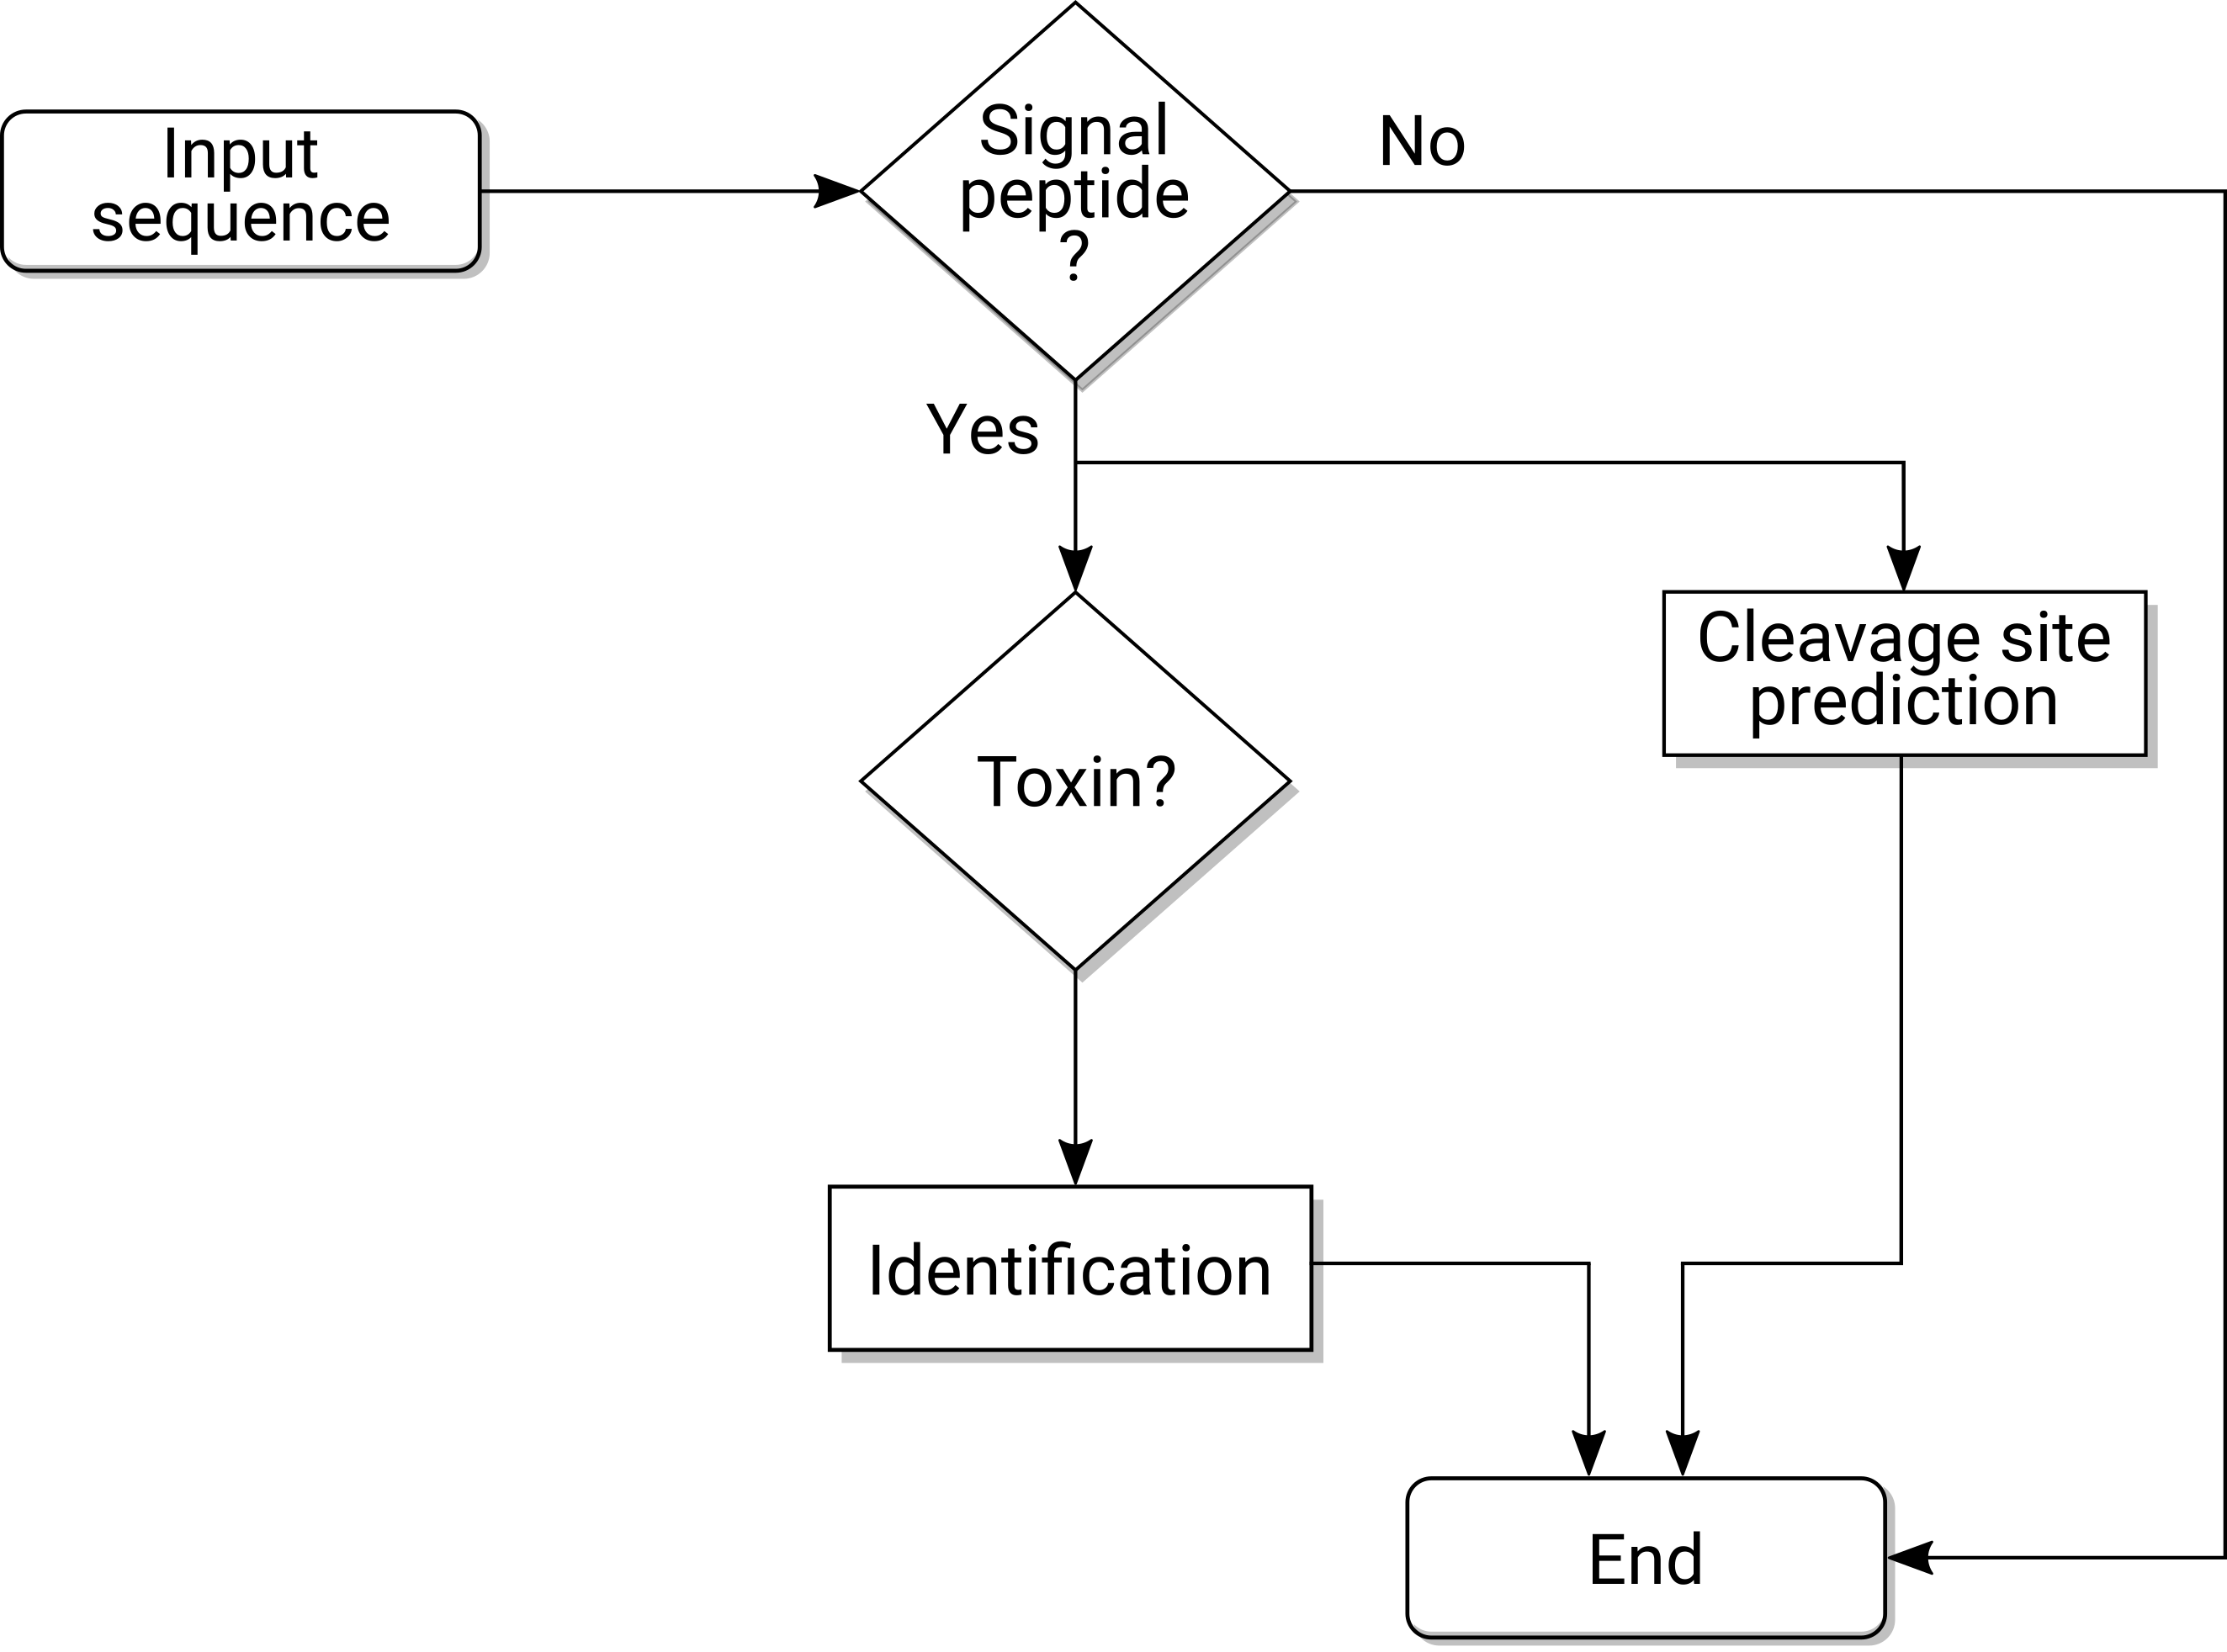
\includegraphics[width=1\textwidth]{chapters/Signal_Peptide/Figures/flowchart-fs8.png}}
% \caption[Flow chart of toxin SP classification using Razor.]{Flow chart of toxin SP classification using Razor.
% }\label{fig:razor_01}
% \end{figure}


\subsection{Statistical analysis}
Data analysis was performed using pandas v1.0.3 \cite{McKinney2010-rg}. Hydrophobicity and SWI were smoothed for the classifier training using the Savitzky-Golay filter implemented in SciPy v1.4.1 \cite{Virtanen2020-fq}. Random forest classifier and MCC computation were done using scikit-learn v0.23.1 \cite{Pedregosa2011-cd}. Plots were generated using Matplotlib v3.1.3 and Seaborn v0.10.0 \cite{Hunter2007-ii,Waskom2020-ye}.


\subsection{Code and data availability}
Jupyter notebooks for reproducing our analyses are available at
https://github.com/\\Gardner-BinfLab/Razor\_paper\_2021. The source code for Razor, our SP annotation server can be found at https://github.com/Gardner-BinfLab/TISIGNER-ReactJS.


% \section{Acknowledgements}
% The authors thank Dr Astra Heywood for providing feedback on the figures and the Razor web application.


% \section{Funding}
% This work was supported in part by the Ministry of Business, Innovation and Employment [MBIE Smart Idea grant: UOOX1709 and MBIE Data Science Programmes grant: UOAX1932], and the Royal Society of New Zealand Te Apārangi [Marsden grant: 19-UOO-040].




\chapter{TISIGNER.com: interactive web services for improving recombinant protein production}
This chapter is adapted from a paper published in Nucleic Acids Research,  the 2021 Web Server Issue \cite{bhandaribk2021-nar-gkab175}. Paul Gardner and Chun Shen Lim provided supervision and feedback. I wrote all the tools under \href{https://tisigner.com}{https://tisigner.com} and did a full stack web developement.


\section{Abstract}
Experiments that are planned using accurate prediction algorithms will
mitigate failures in recombinant protein production. We have developed
TISIGNER \\(https://tisigner.com) with the aim of addressing technical
challenges to recombinant protein production. We offer three web
services, TIsigner (\underline{T}ranslation \underline{I}nitiation
coding region de\underline{signer}), SoDoPE (\underline{So}luble
\underline{Do}main for \underline{P}rotein \underline{E}xpression) and
Razor, which are specialised in synonymous optimisation of recombinant
protein expression, solubility and signal peptide analysis,
respectively. Importantly, TIsigner, SoDoPE and Razor are linked, which
allows users to switch between the tools when optimising genes of
interest.


\section{Introduction}

Recombinant protein production is a key process for life science
research and the development of biotherapeutics. However, low protein
expression and aggregation are the two major bottlenecks of recombinant
protein production \cite{Berlec2013-mb,Esposito2006-tj,Hou2018-yd,Kramer2012-wk,Mazurenko2020-pr,Rosano2014-oq,Vihinen2020-ar}.
Since mRNA abundance alone is insufficient to explain protein abundance \cite{Bernstein2002-gg,Abreu2009-zf,Lim2018-rq,Nieuwkoop2020-ph,Taniguchi2010-uq},
several features of mRNA sequence have been proposed to affect protein expression. 
These features are mostly related to codon usage, such as
the codon adaptation index and tRNA adaptation index
\cite{Brule2017-mx,Reis2004-dl,Gutman1989-pn,Sabi2014-je,Sharp1987-ed},
or measures of mRNA secondary structure, such as G+C content, minimum
free energy (MFE) of RNA secondary structure, and mRNA:ncRNA interaction
avoidance
\cite{De_Smit1990-xy,Dvir2013-lq,Kudla2009-tl,Plotkin2011-ak,Tuller2015-ts,Umu2016-zq}.
Many of these features are not independent, making it challenging to
distinguish the impacts of individual features
\cite{mauger2019mrna}. This, in turn, hinders
the development of accurate prediction/optimisation tools. Recent systematic 
studies suggest that MFE is the most important feature in
protein expression \cite{Cambray2018-kn,mauger2019mrna}. However, more 
recent work shows that the mRNA accessibility of translation initiation sites 
outperforms MFE in predicting relative protein levels from mRNA sequences
\cite{Bhandari2021-wd,Terai2020-co}. Accessibility
is computed by considering all possible structures for a region,
weighted by free energy, not just the single structure with the MFE \cite{Bernhart2006-ma}.

In addition to high protein expression level, high solubility is
preferable for the purification and long-term storage of recombinant
proteins. However, almost half of the successfully expressed proteins
are insoluble
(\href{http://targetdb.rcsb.org/metrics}{http://targetdb.rcsb.org\\/metrics}),
which makes the recombinant protein production process challenging. A
number of methods have been suggested to improve protein solubility, for
example, truncation, mutagenesis, and the use of solubility-enhancing
tags \cite{Chan2010-mo,Costa2014-oe,Esposito2006-tj,Waldo2003-ui}. 
Nevertheless, accurate solubility prediction could save
resources and aid in designing soluble proteins before the experiments.
With these in mind, we have recently formulated the Solubility-Weighted
Index (SWI), which outperforms recent solubility prediction tools based
on machine-learning algorithms
\cite{Bhandari2020-pz}.

Besides, many recombinant proteins of interest are secretory. The
intracellular accumulation of heterologous secretory proteins may be
toxic to the host cells. Therefore, the translocation efficiency of
these proteins plays an important role in the yield quantity and
quality. Secretory proteins usually have a short peptide at the
N-terminus called Signal Peptide (SP) which is responsible for the 
translocation of secretory proteins via the Sec, Signal Recognition Particle
(SRP) or Twin arginine transport (Tat) pathways
\cite{Luirink1994-br,Palmer2012-cw,Rusch2007-it,Von_Heijne1990-sb}.
Detection of SPs or fusion of a suitable SP at the N-terminus is useful
for optimising protein production
\cite{Freudl2018-lr,Karyolaimos2020-gg,Rosano2019-sj,Zamani2015-xj}. In
addition, different pathways have different advantages, for example, the
SRP dependent pathway can be used for rapidly folding proteins
\cite{Owji2018-hg}. However, the Sec dependent
pathway, which is common across all forms of life, has been widely used
for recombinant protein expression because of higher protein production
capacity and quality
\cite{Ma2018-iz,Owji2018-hg}. In addition, the
presence of SPs should almost always be checked when planning the
expression experiments for uncharacterised proteins.

% **************************************************************
% Keep this command to avoid text of first page running into the
% first page footnotes
% \enlargethispage{-65.1pt}
% **************************************************************

Existing web tools predict or optimise either protein expression or
solubility alone
\cite{Agostini2014-te,Chin2014-wu,Grote2005-vr,Puigbo2007-oj,Hebditch2017-bg,Hon2020-gk,Smialowski2012-yg,Sormanni2015-yr,Zayni2018-wc}.
There also exists several web tools for predicting SPs
\cite{Almagro_Armenteros2019-vr,Bagos2009-wh,Hiller2004-gc,Kall2004-te,Savojardo2017-ux}.
Only a very few tools can detect toxic proteins, for example, SpiderP, ClanTox,
and ToxinPred \cite{Gupta2013-fw,Naamati2009-uf,Wong2013-qh}. 
These tools are either limited to predicting the
venoms of certain organisms, such as spiders, or they are not designed
to predict the signal peptides of toxins, rather to predict the toxicity
of mature peptides.
Moreover, these tools are offered through different independent
services. We reasoned these functionalities should be integrated in
order to assist not only in choosing appropriate expression systems, but
also in optimising the expression and solubility levels of recombinant
proteins. Here we present TISIGNER.com that integrates the optimisation
tools TIsigner (\underline{T}ranslation \underline{I}nitiation coding
region de\underline{signer}), SoDoPE (\underline{So}luble
\underline{Do}main for \underline{P}rotein \underline{E}xpression) for
protein expression and solubility, respectively, and Razor for detecting
SPs \cite{Bhandari2021-wd,Bhandari2020-pz,Bhandari2020-oj}. Our web application provides easy, fast and interactive ways to
assist users in planning and designing their experiments (Figure \ref{fig:nar_webserver_fig_1}).

\begin{figure*}[!hbtp]
\begin{center}
\makebox[\textwidth][c]{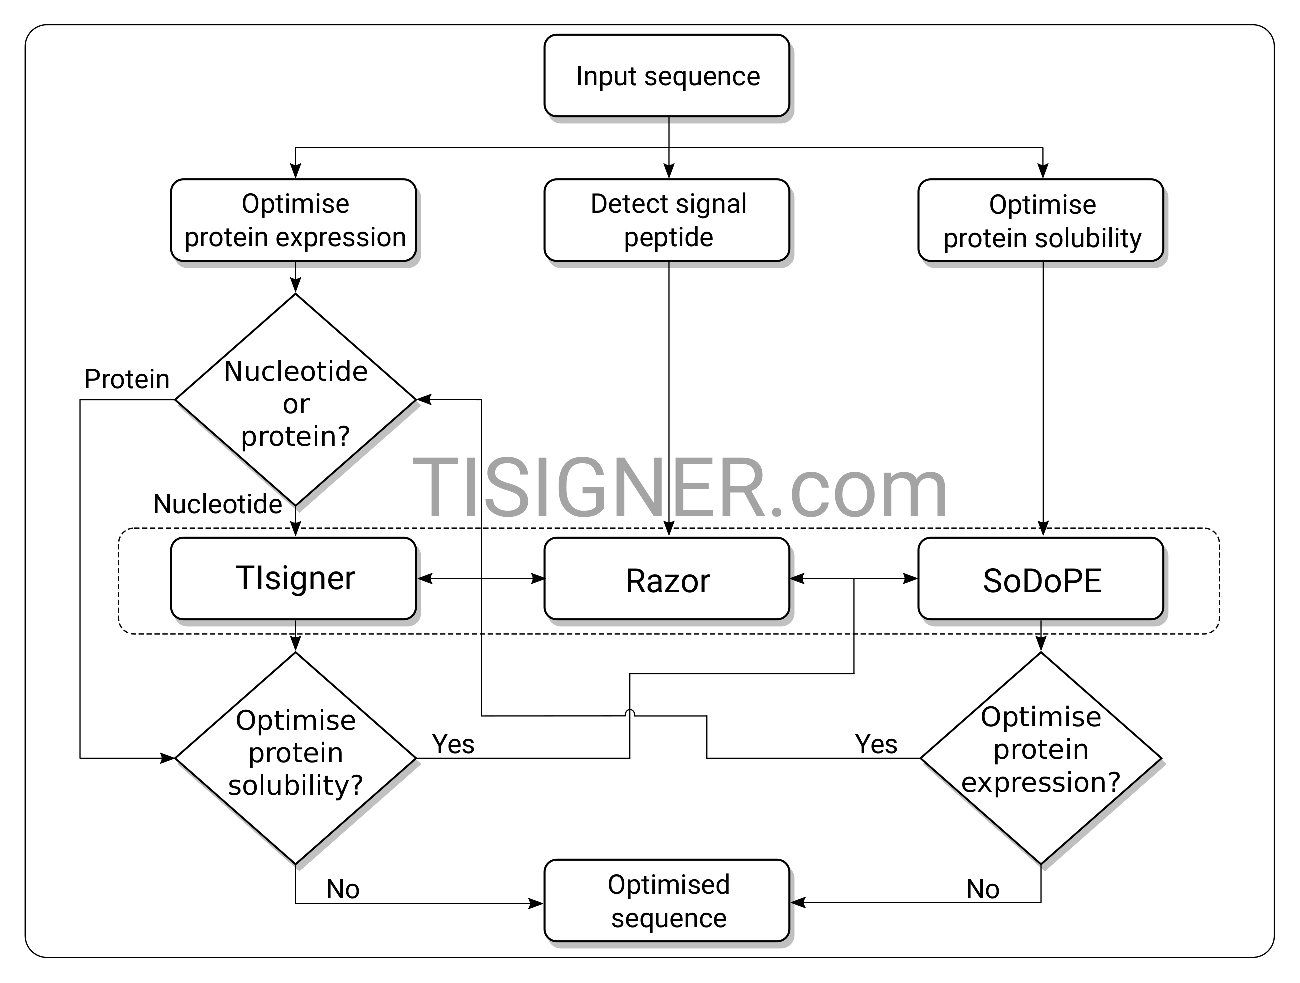
\includegraphics[width=1\textwidth]{chapters/TIsigner_Web/Fig/fig1.eps}}%
\end{center}
\caption[Flow chart for optimising recombinant protein production
using the TISIGNER web application.]{Flow chart for optimising recombinant protein production
using the TISIGNER web application. TIsigner, SoDoPE and Razor are
linked so that protein expression and solubility can be seamlessly
optimised. TIsigner accepts a nucleotide sequence as input, whereas
SoDoPE and Razor accept either a nucleotide or protein sequence. SoDoPE,
\underline{So}luble \underline{Do}main for \underline{P}rotein
\underline{E}xpression; TIsigner, \underline{T}ranslation
\underline{I}nitiation coding region de\underline{signer}.}
\label{fig:nar_webserver_fig_1}
\end{figure*}


\section{Web services}

\subsection{TIsigner}

TIsigner offers tunable protein expression by optimising the mRNA
accessibility of translation initiation sites
\cite{Bhandari2021-wd}. The regions used to
calculate accessibility (opening energy) are specific to the expression
hosts, which is calculated using RNAplfold
\cite{Bernhart2006-ma,Bernhart2011-cc,Lorenz2011-rg}. For
\emph{Escherichia coli}, \emph{Saccharomyces cerevisiae}, and \emph{Mus
musculus} expression hosts, the optimal regions relative to the start
codon for optimisation are $-24:24$, $-7:89$, $-8:11$, respectively. For other
expression hosts, we provide an option `Other', which optimises the
accessibility of the region $−24:89$. Since \emph{E. coli} is the most
popular expression host, the default settings aim to optimise protein
expression in \emph{E. coli} with the T7 lac promoter system (see
below). In this case, only the protein coding sequence is required for
input (Figure \ref{fig:nar_webserver_fig_1}). Otherwise, the 5$^{\prime}$UTR (5$^{\prime}$ 
untranslated region) sequence is also required.



\begin{figure}[!hbtp]
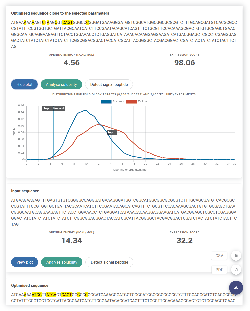
\includegraphics[width=1\textwidth]{chapters/TIsigner_Web/Fig/fig2.pdf}
\caption[The results of TIsigner shows a protein
expression optimised nucleotide sequence.]{The results of TIsigner shows a protein
expression optimised nucleotide sequence. The highlighted nucleotides
show changes made to the input sequence. The opening energy of the input
sequence before and after optimisation is annotated over the
distributions of the opening energy for 8,780 `success' and 2,650 `failure'
experiments from PSI:Biology. Further optimised sequences, if found, are
also displayed. The results can be downloaded in either CSV or PDF
format using the download icon on the bottom right. Each resulting
sequence can be analysed for solubility or signal peptide.}
\label{fig:nar_webserver_fig_2}
\end{figure}

The settings for TIsigner are grouped by complexity (i.e., general,
extra, and advanced). The general settings include the options to modify
the expression host, promoter and target expression score. The target
expression score ranges from $0$ to $100$ (i.e., from the minimum to 
maximum predicted level), which is derived from a logistic regression of 
the opening energy distribution of $11,430$ expression experiments in 
\emph{E. coli} from the `Protein Structure Initiative:Biology' (PSI:Biology) 
\cite{Chen2004-cp,Seiler2014-on}. Hence, this scoring system is only 
applicable to the \emph{E. coli} T7 lac promoter system. Since, there is a non-linear relationship between opening energy and expression score, an interactive plot is also displayed along with the slider to set the target expression score. For other expression 
hosts and promoters, the target expression level can be either maximised or 
minimised (i.e., binary). The extra settings have the options to optimise 
sequence within the translation initiation region or the full-length sequence. 
The AarI, BsaI, BsmBI restriction modification sites are filtered by default, 
whereas other sites can be manually supplied (e.g., a Shine-Dalgarno motif or terminator U-tract). 
The advanced settings allows users to tweak the random seed and sampling 
options (i.e., quick or deep, which uses different numbers of iterations and 
parallel processes). Here users can also customise the region for optimisation 
or disable the terminator checks.

Once the input sequence passes a sanity check, the optimisation task is
rapid ($O(1)$ time using RNAplfold v2.4.11 (using parameters -W
$210$ -u $210$)) with our simulated annealing algorithm. A list of optimised
sequences are returned after checking for terminators using cmsearch
(Infernal v1.1.2)
\cite{Nawrocki2013-te} with RMfam models
\cite{Gardner2015-ui,Kalvari2021-ck}. If
terminators are found, an option to use the full-length sequence for
optimisation will be prompted to users. In a default case (\emph{E.
coli} T7 lac promoter system), the optimised sequence closest to the
chosen expression level is selected as the first solution (Figure \ref{fig:nar_webserver_fig_2}). For other
expression hosts and/or promoters, the optimised sequence with the
minimum changes in nucleotides is selected as the first solution. The
altered nucleotides are highlighted (Figure \ref{fig:nar_webserver_fig_2}). The accessibility of translation
initiation sites for both the input and optimised sequences is shown as
opening energy (kcal/mol). The results can be exported as a PDF or CSV
file. When the default settings are used, the opening energy for each
sequence is indicated on the distributions of the opening energy of
$8,780$ `success' and $2,650$ `failure' groups of the PSI:Biology target
genes. Furthermore, options for solubility and SP analyses using SoDoPE and 
Razor, respectively, are available for each sequence on
the same results page (Figure \ref{fig:nar_webserver_fig_2}).


\subsection{SoDoPE}

SoDoPE is our interactive solubility analysis and optimisation tool
based on the Solubility-Weighted Index (SWI)
\cite{Bhandari2020-pz}. SoDoPE accepts either
a nucleotide or protein sequence (Figure \ref{fig:nar_webserver_fig_1}). Upon submission, a query is
sent to the HMMER web service for domain annotation
\cite{Potter2018-ox}. Successful annotations
are displayed as interactive graphics, in which the annotated domains
are represented as discorectangles, above a grey band that represents
the input protein sequence (Figure \ref{fig:nar_webserver_fig_3}). Information about a protein domain is shown
upon a mouse hover. The domains can be selected for solubility
analysis. For a complete domain annotation report, a link to the HMMER
results page is also provided.

\begin{figure}[!hbtp]
\includegraphics[width=1\textwidth]{chapters/TIsigner_Web/Fig/fig3.pdf}
\caption[Exploring and optimising protein solubility using SoDoPE interactive
graphics.]{Exploring and optimising protein solubility using SoDoPE interactive
graphics. Upon clicking a protein domain or selecting a region of
interest, its solubility is optimised in real-time, and a list of
regions with extended boundaries and higher probabilities of solubility
is returned as green buttons (clickable). The probabilities of
solubility of the selected region with and without fusion tags can be
visualised in a barplot. The flexibility and hydrophobicity profile
plots for the selected region can also be selectively viewed. The
sequence can also be checked for the presence of a signal peptide or
optimised for protein expression.}
\label{fig:nar_webserver_fig_3}
\end{figure}

In addition, a two-way slider is available for navigation through any
region of interest (Figure \ref{fig:nar_webserver_fig_3}). The probability of solubility, flexibility and GRAVY
(GRand AVerage of hydropathicitY) is shown in real-time according to the
user-selected region. The selected region is optimised for higher
solubility using simulated annealing. Only the regions with extended
boundaries and also higher probability of solubility is returned. SP
analysis can also be done using Razor (see below).

A profile plot of flexibility and/or hydrophilicity corresponding to the
user selected region is generated (Figure \ref{fig:nar_webserver_fig_3}). This allows an estimation of
rigid/flexible regions and possible helices, that may be helpful for
mutagenesis experiments. The sequence of the selected region is shown,
with the option of sequence conversion between nucleotide and amino acid
sequence format. In particular, the nucleotide sequence can be
redirected to TIsigner for optimising protein expression (Figure \ref{fig:nar_webserver_fig_1} and \ref{fig:nar_webserver_fig_3}, through the `view DNA \textbar\ optimise expression' button).

The contributions of several solubility-enhancing tags to user selected
regions can be compared and shown in a bar plot, including thioredoxin
(TRX), maltose binding protein (MBP), small ubiquitin-related modifier
(SUMO) and glutathione S-transferase (GST) tags (Figure \ref{fig:nar_webserver_fig_3}). Users can also input a
fusion sequence of interest either in a nucleotide or protein sequence
format.

% **************************************************************
% Keep this command to avoid text of first page running into the
% first page footnotes
% \enlargethispage{-65.1pt}
% **************************************************************

\subsection{Razor}

Razor is our SP prediction tool which is based upon random forest models
of protein features from the eukaryotic SP sequences of the SignalP 5.0
dataset and the animal toxin annotation project
\cite{Almagro_Armenteros2019-vr,Bhandari2020-oj,Jungo2012-ja}. Razor accepts
either a protein or a nucleotide sequence (Figure \ref{fig:nar_webserver_fig_1}). After validation, the
N-terminal region is checked for the presence of a SP using five random
forest models. This gives five SP scores (S-scores) for a given
sequence. For detecting the cleavage site, we use a sliding window of $30$
residues and our optimised weight matrix for residues around the
cleavage site. The scored subsequences are scored by additional five
random forest models to give the cleavage site scores (C-scores) along
the sequence, which is displayed as a step plot (Figure \ref{fig:nar_webserver_fig_4}). The Y-score, which is
the geometric mean of S-scores and the max of C-scores, is used to infer
whether the given sequence has a SP or not. The median of these five
Y-scores is displayed as the final score. The cleavage site from the
model with the median of max of C-scores is used to annotate the
predicted region.

\begin{figure}[!hbtp]
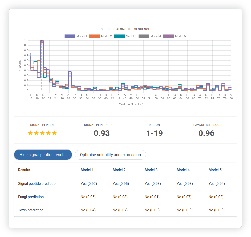
\includegraphics[width=1\textwidth]{chapters/TIsigner_Web/Fig/fig4.pdf}
\caption[Detection of signal
peptides using Razor.]{Detection of signal
peptides using Razor. The dotted annotation in the step plot for the
cleavage site scores (C-scores) shows the most likely position for
proteolytic cleavage. The sequence can also be checked and optimised for protein
solubility and expression.}
\label{fig:nar_webserver_fig_4}
\end{figure}


If any of the models detect a SP in the input sequence, we further check
whether the SP belongs to toxins, using five random forests trained on
toxin-specific SPs. The final toxin score is the median of scores from
those random forest models. Furthermore, since we noticed a lack of
tools specialising in predicting SPs from fungi, any detected signal
peptide is checked for such origin. Similarly, we use five random
forests for detecting fungal SPs, with the final fungal score being the
median score of these models. This random forest is built using residue composition of the signal sequence. Since we have five random forest models in
each step (SP, toxin- and fungal-specific SP detection steps), stars are displayed as an
indication of the number of models agreeing on the sequence falling on
either category (Figure \ref{fig:nar_webserver_fig_4}).

Razor is linked with SoDoPE for checking and optimising protein
solubility (Figure \ref{fig:nar_webserver_fig_4}). If a nucleotide sequence was submitted, this sequence can
also be optimised for protein expression using TIsigner (Figure \ref{fig:nar_webserver_fig_1}).


\section{Discussion}
Low protein expression and solubility are the major hindrances to a successful recombinant protein production. Based on our comprehensive studies on these two problems, we have developed novel tools to optimise protein expression (TIsigner) and solubility (SoDoPE), and assessed their predictive performance using independent datasets (Table \ref{tab:Summary_of_TIsigner_and_SoDoPE}). Our tools offer some unique features in an interactive way. TIsigner allows tuning of protein expression from low to high levels, whereas SoDoPE allows easy navigation of protein sequence/domains with real-time solubility prediction. Based on our assessment of similar tools, none of the publicly available tools provides these features.

Our third tool, Razor, is designed to check the presence of SPs. Compared to other related tools, Razor also predicts toxin- and fungal-specific SPs (Table \ref{tab:Summary_of_Razor}). These would be helpful for users in choosing the expression and purification systems that prevent the harmful intracellular accumulation of recombinant secretory proteins/toxins. 

Our tools are interactive, fast, and accurate. Importantly, our tools are highly integrated, allowing a seamless transition between the optimisation tools. To make such transition intuitive, our web services limits one input sequence at a time and we aim to remove this input sequence limitation in the future. For optimising a large number of sequence, we provide the command-line version of each of our tools (see below).


\section{General information}

Demo input and results are available for new users to get started. A
list of frequently asked questions is also available for each tool. The
frontend is written in React and uses responsive web design principles.
The backend is written in Flask and Python v3.6. The website is hosted on
a virtual machine (Red Hat Enterprise Linux 8) running on Intel Xeon (8
${\times}$ 2.60 GHz) with 4GiB RAM, by the Information Technology Services at the
University of Otago.


\section{Data availability}

The web server is available at \href{https://tisigner.com}{https://tisigner.com}. This website is free
and open to all users and there is no login required. All our tools, and the website 
are open-sourced (\href{https://github.com/Gardner-BinfLab/TISIGNER-ReactJS}{https://github.com/Gardner-BinfLab/TISIGNER-ReactJS};\\ \href{https://github.com/Gardner-BinfLab/TIsigner/tree/master/TIsigner\_cmd}{https://github.com/Gardner-BinfLab/TIsigner/tree/master/TIsigner\_cmd};\\ \href{https://github\\.com/Gardner-BinfLab/SoDoPE\_paper\_2020/tree/master/SWI}{https://github.com/Gardner-BinfLab/SoDoPE\_paper\_2020/tree/master/SWI};\\ \href{https://github.com/Gardner-BinfLab/Razor}{https://github.com/Gardner-BinfLab/Razor}) and privacy friendly (no user data stored).


% \section{Acknowledgements}

% This work was supported in part by the Ministry of Business, Innovation
% and Employment {[}MBIE Smart Idea grant: UOOX1709 and MBIE Data Science
% Programmes grant: UOAX1932{]}, and the Royal Society of New Zealand Te
% Apārangi {[}Marsden grant: 19-UOO-040{]}.


\chapter{Discussion}
Recombinant protein production is widely used in scientific research and industry. However, in general, the success rate of these experiments is around a 25\%, the 75\% failure rate is attributed to protein expression and solubility. In this work, we studied the major factors affecting these two steps and used the findings to develop methods to optimise the protein production. In addition, since many recombinant proteins of interest are secretory, translocation efficiency also plays an important role in the final yield. Since protein translocation is usually performed by signal peptides, fusing appropriate signal peptide to the protein of interest increases the yield. Therefore, we also developed tool to predict the presence of signal peptide in the sequence and identify the mature peptide. 

\section{Optimising protein expression using TIsigner (Translation Initiation coding region designer)}
We have demonstrated that mRNA accessibility is a better predictor of protein expression across several datasets (Table \ref{tab:Summary_of_TIsigner_and_SoDoPE}). Therefore, we used this feature to develop, TIsigner (\href{https://tisigner.com/tisigner}{https://tisigner.com/tisigner}), a tool for optimising protein expression. TIsigner uses a simulated annealing algorithm to provide a novel mechanism for tuning the protein expression from low to high levels. Other unique features include an estimation of protein expression for mRNA sequences, which we've named as 'expression score' and synonymous changes limited to the first 10 codons of the input sequence. TIsigner's synonymous substitution algorithm is designed to make a minimal number of changes. This approach is advantageous for two reasons\textemdash first, it is possible to do a PCR cloning using the optimised part as primers, which in turn reduces the cost of the experiment significantly as compared to the conventional full gene synthesis method. Second, it reduces the possibility of generating toxic mRNA sequences. mRNA toxicity is still a difficult problem to address and the mechanisms of toxicity are not fully understood yet \cite{mittal2018codon}. However, TIsigner offers a possibility to do synonymous changes over all codons, which may be useful if terminators are found. The web-version of TIsigner automatically suggests doing a full length substitution if any terminators are found (Figure \ref{fig:terminator_prompt}).

\begin{figure}[htbp!]
\center
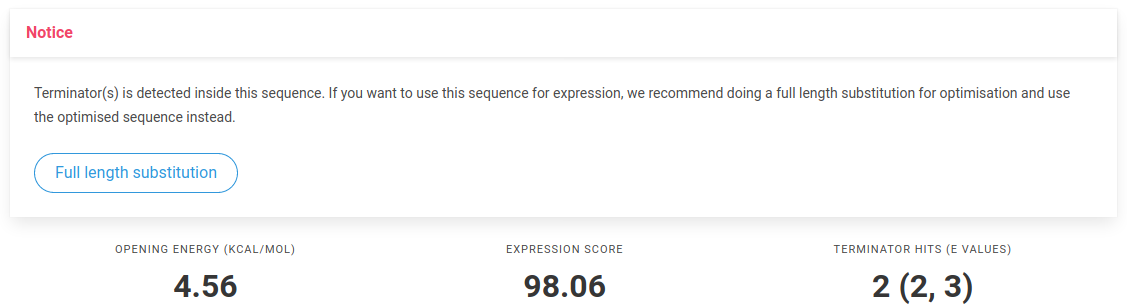
\includegraphics[width=1\textwidth]{chapters/Discussion/Figures/terminator_prompt.png}
\caption[TIsigner suggests to do a full length substitution if any transcription terminators are found in the sequence.]{\textbf{TIsigner suggests to do a full length substitution if any transcription terminators are found in the sequence.} Mock data was used for demonstration purposes.}%the List of Figures because of the *}
\label{fig:terminator_prompt}
\end{figure}


\section{Optimising protein solubility using SoDoPE (Soluble Domains for Protein Expression)}
Almost all use cases of protein require a soluble product. Hence, optimising just protein expression is not sufficient for a better protein production. Based on protein structural flexibility, which is the most accurate predictor of solubility among all conventional features, we have developed a new metric called the Solubility-Weighted Index (SWI). SWI is a very accurate predictor of solubility and outperforms other tools (Table: \ref{tab:Summary_of_TIsigner_and_SoDoPE}). Using SWI, we developed a solubility prediction and optimisation tool, SoDoPE (\href{https://tisigner.com/sodope}{https://tisigner.com/sodope}). SoDoPE is an unparalleled tool with a distinctive interface for an easy navigation of protein sequence/domains with real-time solubility prediction and optimisation. The effect of different solubility tags on solubility can also be compared to pick the best one for experiment.


\section{Detection of signal peptides using Razor}
The presence of signal peptides should almost always be checked when planning expression experiments for uncharacterised proteins. Based on the properties of signal sequences, we developed Razor (\href{https://tisigner.com/razor}{https://tisigner.com/razor}) to detect the presence of N-terminal signal peptides. Compared to other related tools, Razor also predicts toxin and fungi\textemdash specific SPs. These would be helpful for users in choosing the expression and purification systems that prevent the harmful intracellular accumulation of recombinant secretory proteins/toxins. The performance summary of Razor is given in Table \ref{tab:Summary_of_Razor}.



\section{Reception of tools by the community}
TISIGNER (\href{https://tisigner.otago.ac.nz}{https://tisigner.otago.ac.nz}, \href{https://tisigner.com}{https://tisigner.com}, \href{https://tisigner.nz}{https://tisigner.nz}) is the web-suite for these tools. Initially, it consisted of TIsigner only, hence the name, but has been expanded to include both SoDoPE and Razor. Our tool has been online since February 2020. Despite the short period (March 2021 at the time of writing), our tools are gaining traction among researchers worldwide, with an exponential increase in the numbers of visitors from many countries (Figure \ref{fig:tisigner_stats}).


\begin{figure}[H]
\center
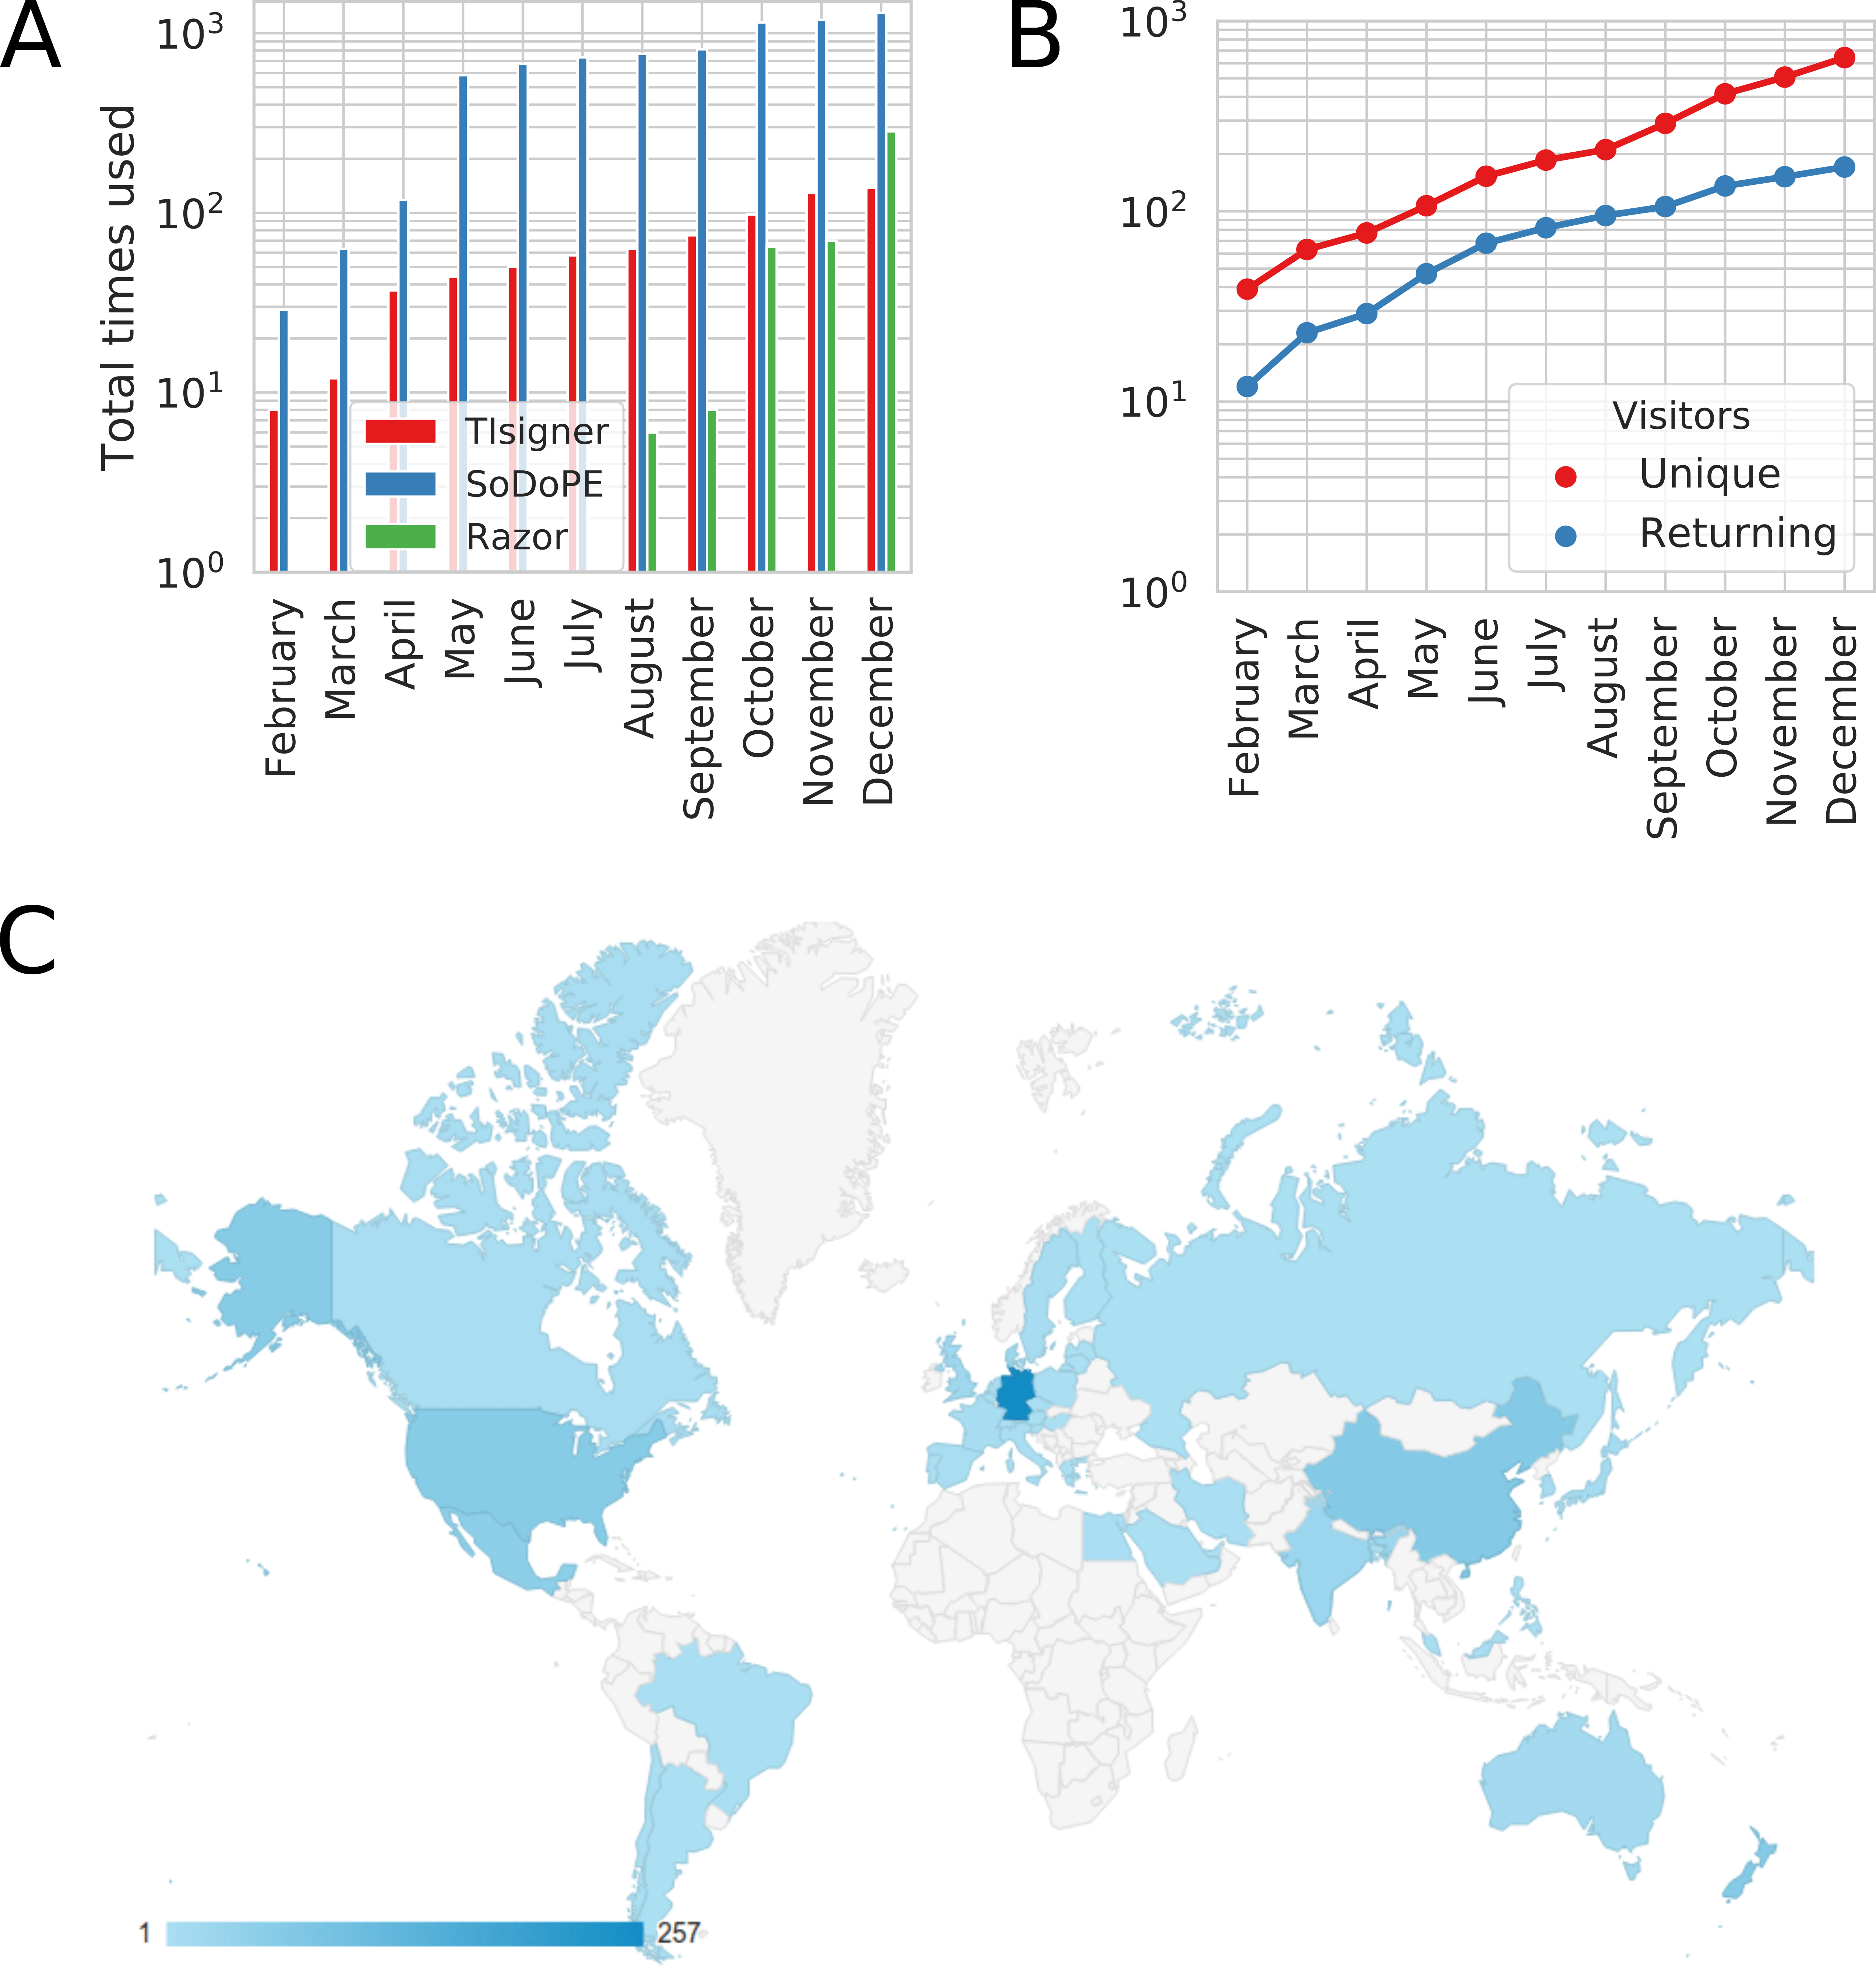
\includegraphics[width=0.8\textwidth]{chapters/Discussion/Figures/tisigner_stats.png}
\caption[TISIGNER.com web service is getting popular among researchers worldwide.]{\textbf{TISIGNER.com web service is getting popular among researchers worldwide. (A)} Number of times each tool was used in a logarithmic scale. \textbf{(B)} The number of unique and returning visitors in a logarithmic scale. \textbf{(C)} Geographical location of users. Data is for the period of February 2020 to March 2021 from Google Analytics (\href{https://analytics.google.com}{https://analytics.google.com}). }%the List of Figures because of the *}
\label{fig:tisigner_stats}
\end{figure}


\section{Outlook}
Tthe present work enumerates some of the cellular level processes responsible in protein synthesis. In this section, we will use a simplified version of higher level modelling by taking into account of the production system as a black-box (S) which has various levels of noise and uncertainties. In such a crowded environment, there might be some, possibly unknown, additional constrain and feedback between or within the cells, which could stabilise or destabilise the production system. Let us represent any and all of these uncertainties, noises and feedbacks collectively by a black-box (F) and simply refer to as feedbacks. A stable system is a result of interplay between the system and its feedback. These type of systems are called \textit{control systems} (Figure \ref{fig:control_system}A). The output behaviour of output of these systems when the input is switched from low to high is studied within the framework of step response.

\begin{figure}[htbp!]
\center
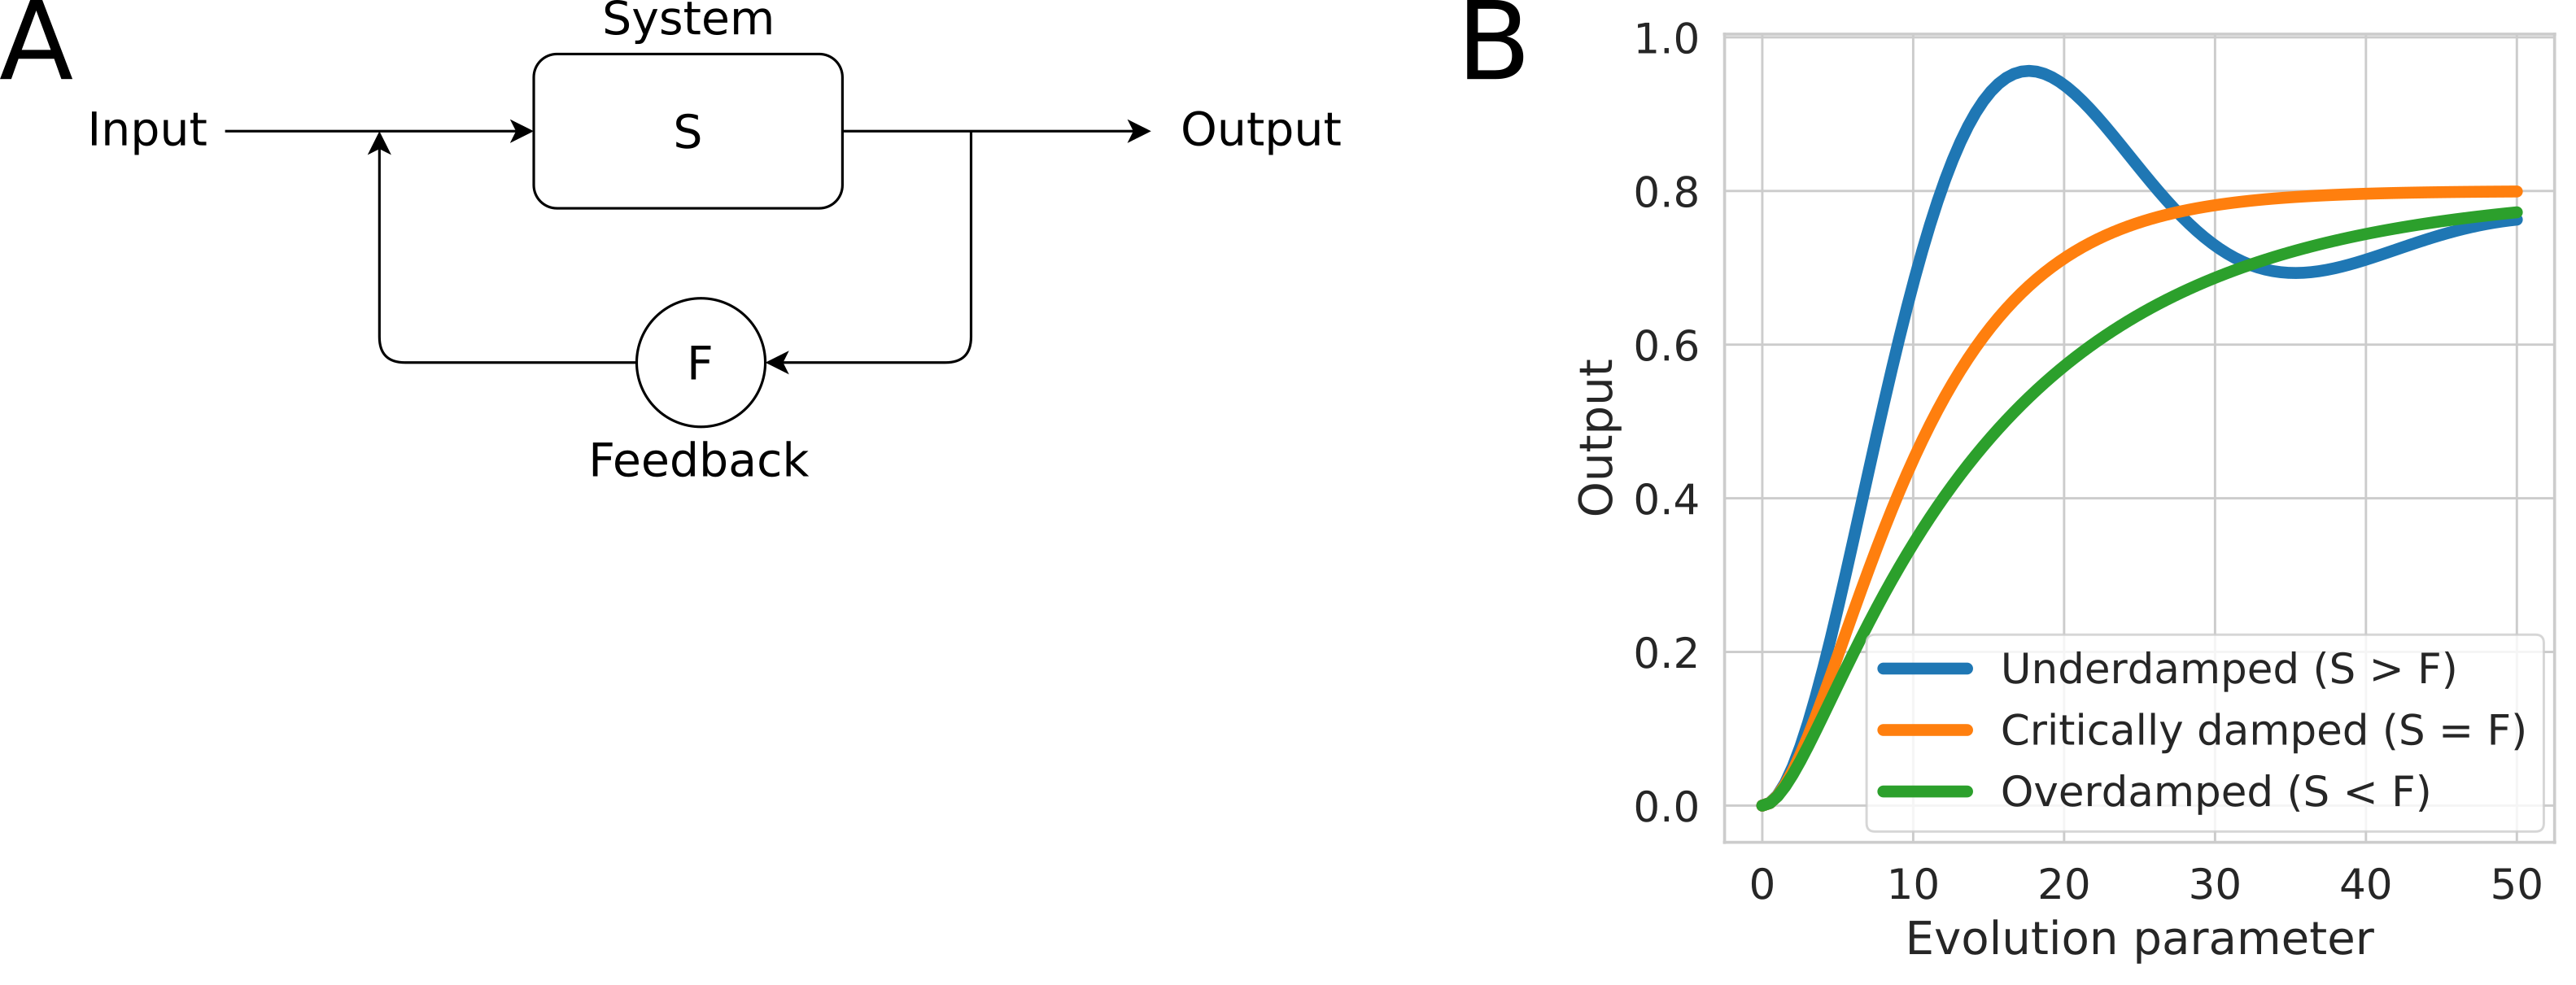
\includegraphics[width=1\textwidth]{chapters/Discussion/Figures/control_system.png}
\caption[Different possible step responses of a stable control system when input is switched from low to high.]{\textbf{Different possible step responses of a stable control system when input is switched from low to high. (A)} A control system (S) with a feedback loop (F). This system is assumed to be stable. \textbf{(B)} Output (step response) when the damping effects due to feedback (F) are low, equal and high compared to the system (S). Evolution parameter is an arbitrary parameter of the system.}%the List of Figures because of the *}
\label{fig:control_system}
\end{figure}

In control theory, the evolution of higher order system with respect to some evolution parameter (often time, but could be any other variable) is approximated by a second order ordinary differential equation: 
\begin{equation}
    \Ddot{x} + 2\zeta\omega_n\dot{x} + \omega_n^2 x = 0
\end{equation}
where $\omega_n$ is the eigen frequency, $\zeta$ is the damping ratio. The eigen frequency is the frequency at which the system oscillates when no external forces are present, whereas damping ratio is an indicative of the relative strength of feedback to the system (F/S). The most general solution of this equation can be written as a linear combination:
\begin{equation}
    x = Ce^{-\omega_n(\zeta + i\sqrt{1-\zeta^2})} + De^{-\omega_n(\zeta - i\sqrt{1-\zeta^2})}
\end{equation}

Hence for any system, multiple output possibilities exist which are shown in Figure \ref{fig:control_system}B. For $0 \leq \zeta < 1 $, the output is decaying exponential with oscillations and is called underdamped. For $\zeta > 1$, the system does not oscillate and is called overdamped whereas for $\zeta = 1$, the system is logistic in nature and is called critically damped. 



% Documents/Thesis/Committee_Meeting_April_2020/Jupyter_Notebook/NonLinearRegression/For_Thesis.ipynb
\begin{wrapfigure}{r}{0.5\textwidth}
  \begin{center}
    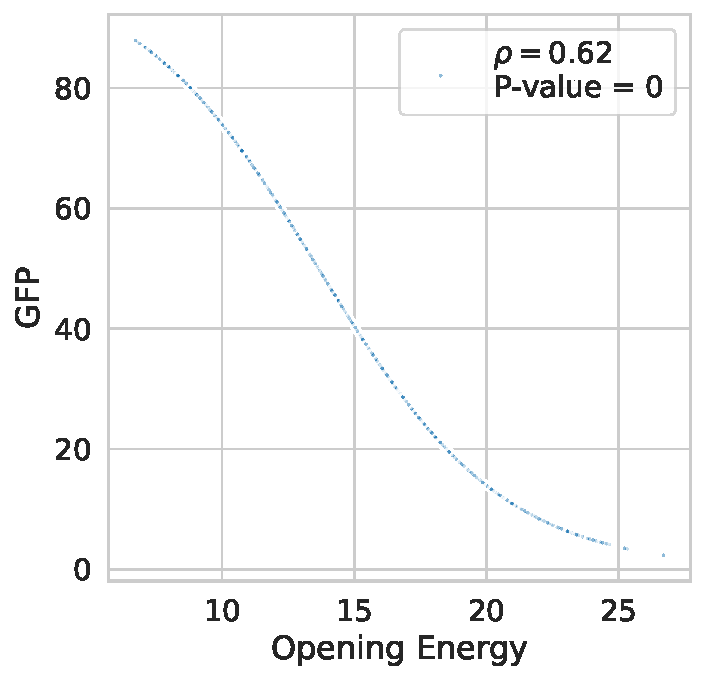
\includegraphics[width=0.5\textwidth]{chapters/Discussion/Figures/cambray_fitting.pdf}
    \caption[Best fit shows an overdamped ($\zeta > 1$) trend in GFP data from Cambray \textit{et al.}]{\textbf{Best fit shows an overdamped ($\zeta > 1$) trend in GFP data from Cambray \textit{et al.} (2018)} Spearman's $\rho = 0.62$, P-value is less than machine's underflow. In these type of systems, the output increases steadily with an increase in input level. Reverse trend is because lower opening energy are more optimal than higher opening energy sequences. }%the List of Figures because of the *}The opening energy of the region (-24:24) is used.
    \label{fig:refitting_data_cambray}
  \end{center}
\end{wrapfigure}

Ideally, physical systems with $\zeta = 1$ (critically damped) are preferred because the maximum output can be reached easily. In contrast, biological systems are often noisy, which could make the output behave like either of the cases. As an illustration, the data from Cambray \textit{et al.} \cite{Cambray2018-kn}, follows an overdamped trend ($\zeta > 1$) (Figure \ref{fig:refitting_data_cambray}). However, the results of our GFP experiments using TIsigner, fits better to the underdamped system ($0 \leq \zeta < 1 $) than a logistic regression (critically damped) (Figure \ref{fig:refitting_data_tisigner}). In this case, the output tends to oscillate when the input is increased beyond a certain limit, which we observed (Figure \ref{fig:refitting_data_tisigner}C).


% Documents/Thesis/Committee_Meeting_April_2020/Jupyter_Notebook/NonLinearRegression/For_Thesis.ipynb
\begin{figure}[htbp!]
\center
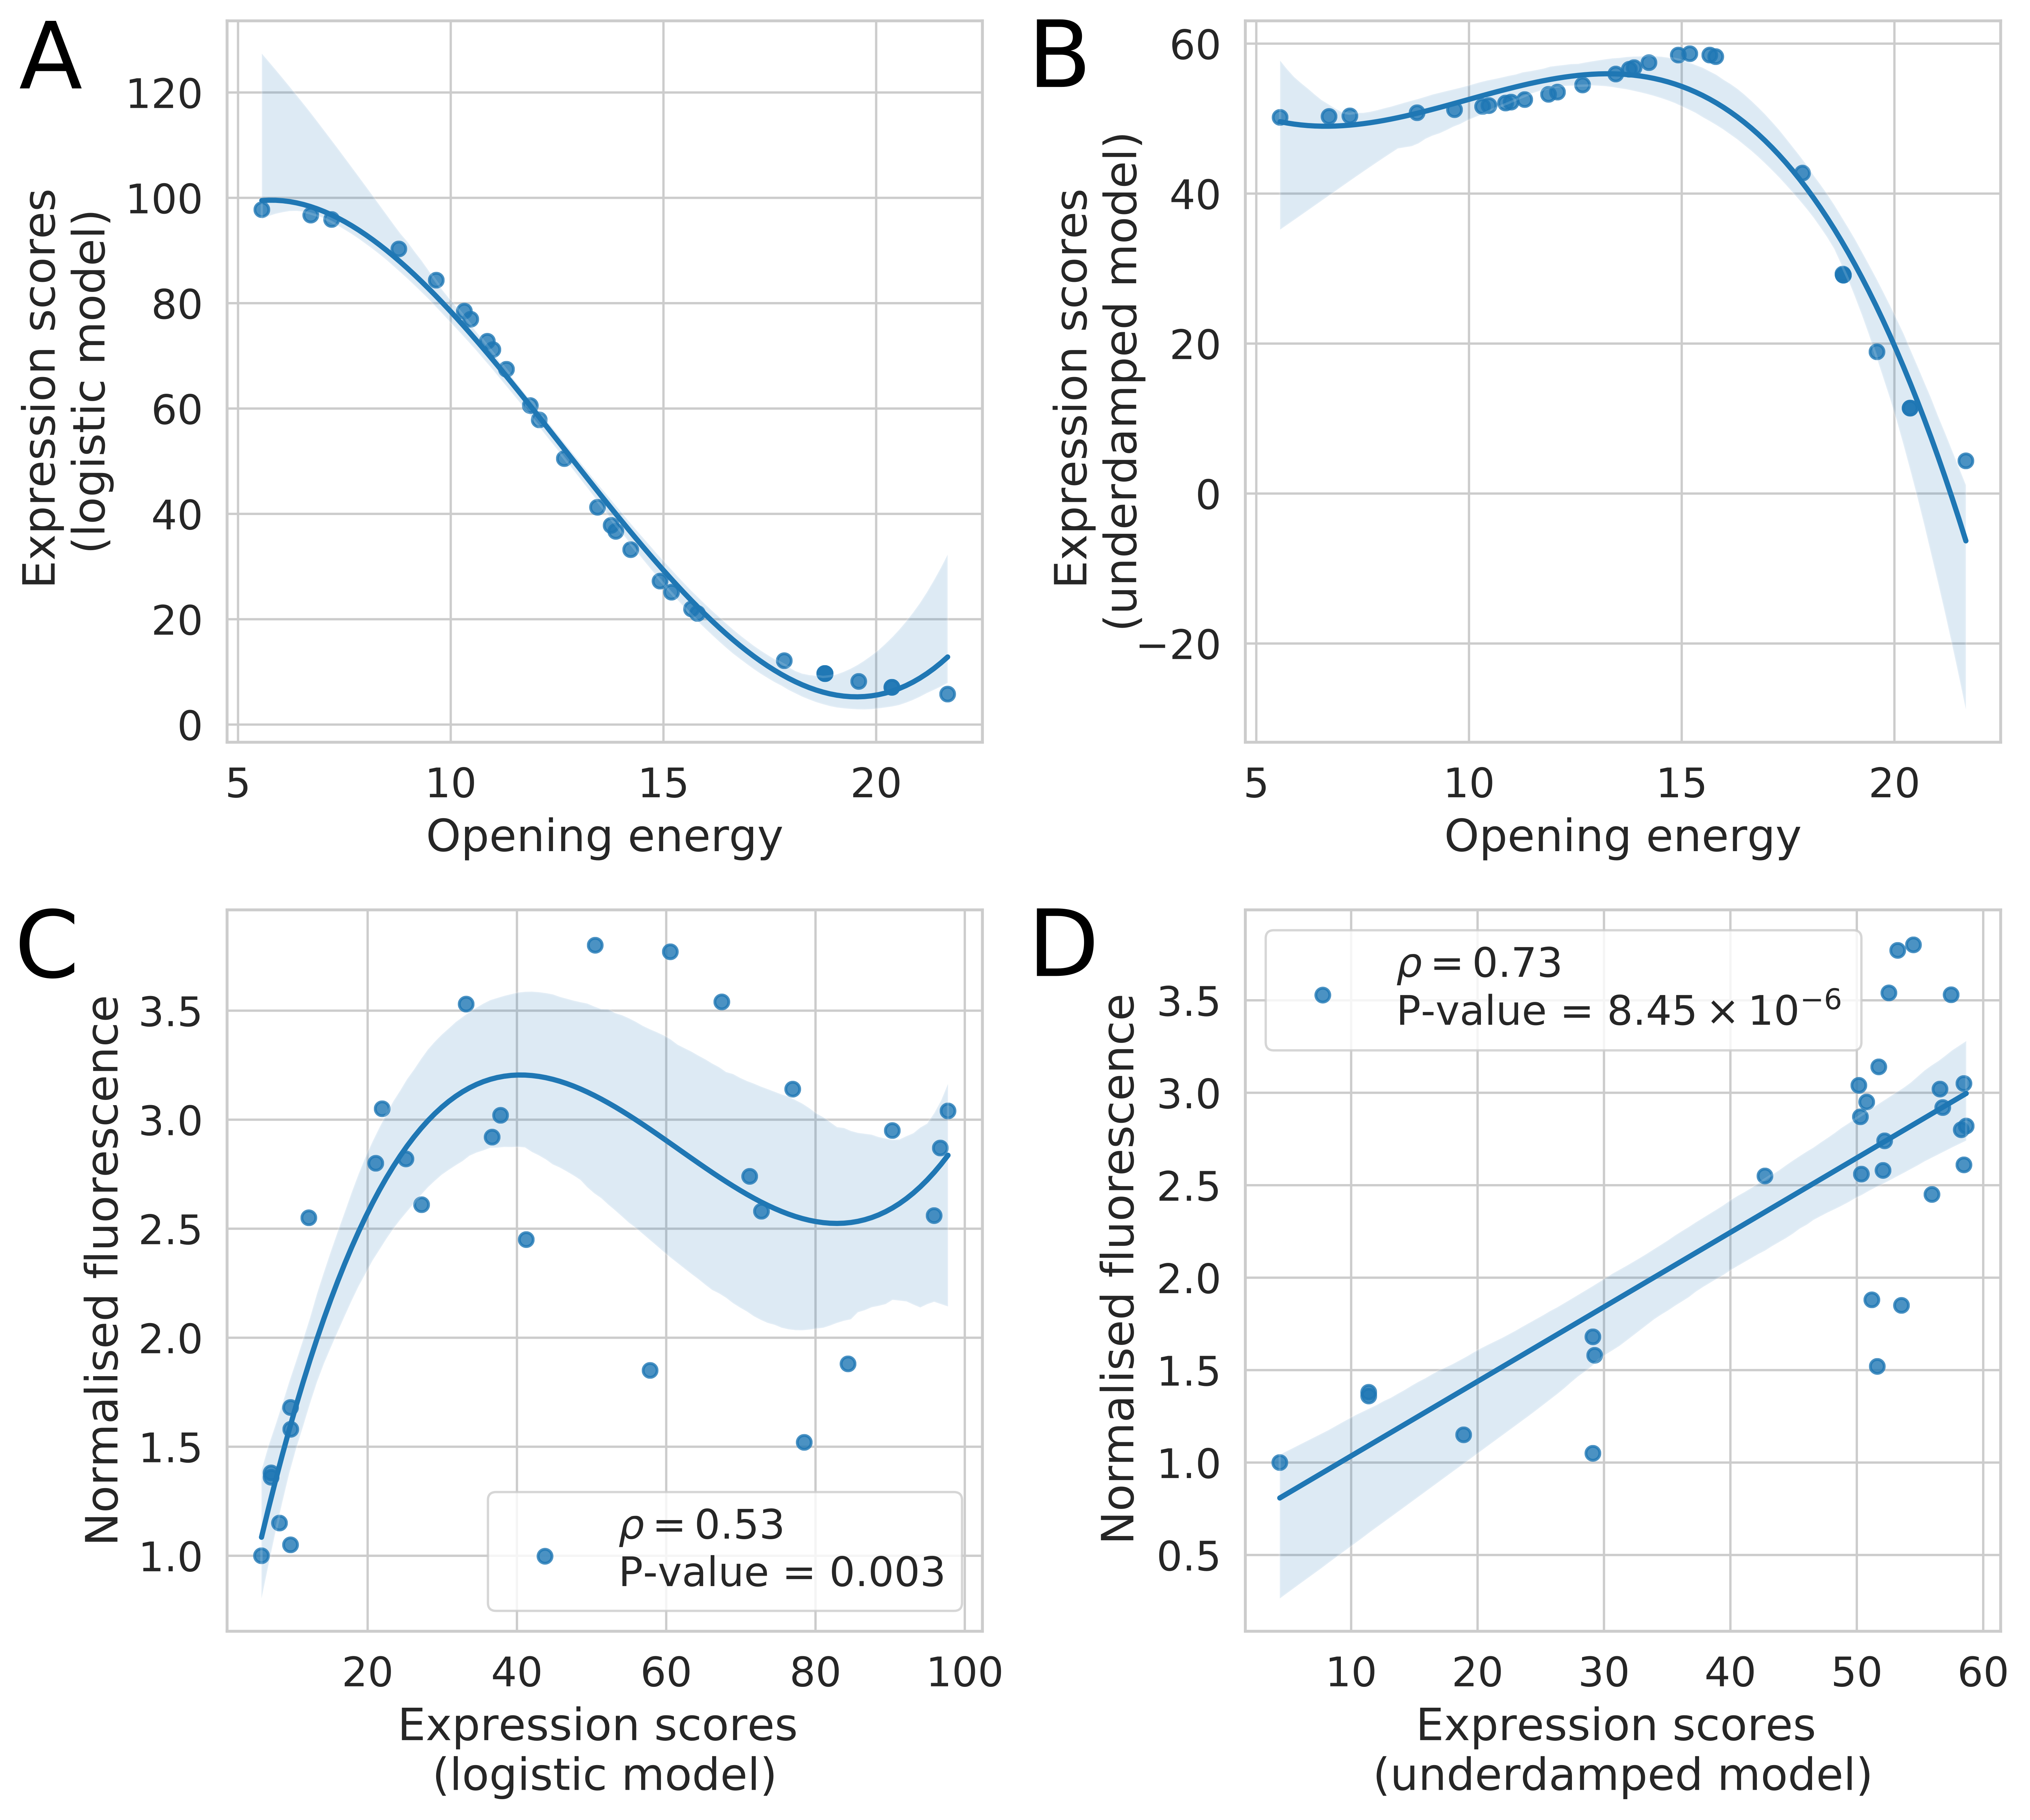
\includegraphics[width=0.9\textwidth]{chapters/Discussion/Figures/refitting_tisigner.png}
\caption[An underdamped model fits better to the TIsigner experimental data (GFP) than a logistic (critically damped) model.]{\textbf{An underdamped model fits better to the TIsigner experimental data (GFP) than a logistic (critically damped) model.} The conversion of opening energy to expression score using \textbf{(A)} logistic (critically damped) model and  \textbf{(B)} underdamped model. Spearman'r $\rho$ between normalised fluorescence and expression scores derived from \textbf{(C)} logistic model and \textbf{(D)} underdamped model. Spearman's $\rho$ is stronger when we model the production as underdamped (0.73, P-value=$8.45\times 10^{-6}$) compared to the critically damped model (0.53, P-value=0.003). Lines represent the best fit regression.}%the List of Figures because of the *}
\label{fig:refitting_data_tisigner}
\end{figure}

 These inherent and inevitable feedbacks and constrains, for example protein toxicity and solubility issues, may be different for different systems, protein of interest and protocols. In this work, these issues were treated separately. However, modelling the production system by taking into account of all these variables may be required to explain the outcomes of recombinant protein production systems with a greater accuracy. The simulated production system (Fig \ref{fig:tisigner_fig4}), which takes into account of only the protein toxicity and mRNA accessibility, was surprisingly close to the experimental results. Combined with a higher order modelling as outlined above, such simulations can be used to explore and study the effects of different features of mRNA and protein as well as stochasticity. Nevertheless, this work provides a sufficient background for such a complex modelling in the future.
 
 
%  The results from the simulation in (Fig \ref{fig:tisigner_fig4}), which takes into account of protein toxicity and mRNA accessibility, was surprisingly close to the experimental results. Such simulations and modelling can be used to explore the effects of many mRNA and protein features as well as stochasticity. Nevertheless, this work provides a sufficient background for such complex modelling in the future. 
 
   


% \section{Future work and outlook}



\appendix

\chapter{Protein yield is tunable by synonymous codon changes of translation initiation sites}
\section{Supplementary notes}

\subsection{Cloning of TIsigner variants of GFP and Luciferase}
The cloning of TIsigner sequence variants for E. coli expression was performed using the MIDAS Golden Gate cloning system \cite{Van_Dolleweerd2018-pw}. As with other Golden Gate assembly (GGA) systems, MIDAS is a modular, hierarchical DNA assembly system that uses the Type IIS restriction enzymes AarI, BsaI and BsmBI to assemble genes, transcription units and other devices from basic parts, and subsequently enables multiple devices to be assembled together on a single plasmid.
As per MIDAS, basic parts such as promoters, coding sequences and terminators were amplified by PCR or ordered as synthetic polynucleotide sequences from gene synthesis companies. The basic parts are listed in Table S1. Protocols for the GGA reactions are as described in van Dolleweerd et al., 2018 \cite{Van_Dolleweerd2018-pw}.

\subsubsection{N-terminal region of GFP (GFPN)}
Overlapping oligonucleotide primer pairs corresponding to the first ten codons of each of the gfp sequence variants produced by the TIsigner algorithm were ordered from Integrated DNA Technologies (IDT) (see Table S2). Each overlapping pair of primers was annealed together and used as a template for amplification by Q5 polymerase (New England Biolabs) to create a double-stranded DNA product spanning the N-terminal region of GFP (GFPN; codons 1 to 10; see Fig S1), and with MIDAS [CCAT] prefix and [GTTG] suffix nucleotides.

\subsubsection{C-terminal region of GFP (GFPC)}
The C-terminal region of GFP (designated GFPC), spanning codons 11 to 238 of the native gfp of \textit{Aequoria victoria}, was synthesized (GeneArt) with flanking BsmBI recognition sites, and with the [GTTG] MIDAS prefix (compatible with the [GTTG] suffix on the GFPN part) and [GCTT] suffix nucleotides.

\subsubsection{N-terminal region of luciferase (RLucN)}
Overlapping oligonucleotide primer pairs corresponding to the first ten codons of each of the luciferase sequence variants generated by the TIsigner algorithm were ordered from Integrated DNA Technologies (IDT) (see Table S3). Each overlapping pair of primers was annealed together and used as a template for amplification by Q5 polymerase (New England Biolabs) to create a double-stranded DNA product spanning the N-terminal region of luciferase (RLucN; codons 1 to 10), and with a MIDAS [CCAT] prefix and an [AGGA] suffix.

\subsubsection{C-terminal region of luciferase (RLucC)}
The C-terminal region of luciferase (designated RLucC), spanning codons 11 to 311 of the native luciferase of \textit{Renilla reniformis}, was amplified from the full-length, native luciferase sequence (synthesized by GeneArt) using primers that add flanking BsmBI recognition sites, and a MIDAS [AGGA] prefix (compatible with the [AGGA] suffix on the RLucN part) and a [GCTT] suffix.


\subsubsection{MIDAS Level-1 cloning of parts}
PCR products, purified using commercially available column-based protocols (Macherey-Nagel), or parts produced by gene synthesis were cloned into the MIDAS pML1 vector by BsmBI-mediated Golden Gate assembly (BsmBI-GGA). As per the MIDAS design, BsmBI-GGA into the pML1 vector results in elimination of the BsmBI recognition sites and each part becomes flanked by BsaI recognition sites that cleave at the MIDAS prefix and suffix nucleotides.

In the case of the \textit{Aequoria victoria} gfp TIsigner variants, each GFPN part cloned into the pML1 vector becomes flanked by BsaI recognition sites that are cleaved at the [CCAT] prefix and [GTTG] suffix (Fig S2). Cloning of the GFPC part into the pML1 vector results in a GFPC module flanked by BsaI recognition sites that are cleaved at the [GTTG] prefix and at the [GCTT] suffix (Fig S3).

In the case of the \textit{Renilla reniformis} luciferase TIsigner variants, each RLucN part cloned into the pML1 vector becomes flanked by BsaI recognition sites that are cleaved at the [CCAT] prefix and [AGGA] suffix, while the C-terminal fragment, RLucC, becomes flanked by BsaI recognition sites that generate an [AGGA] prefix and a [GCTT] suffix upon cleavage.

All parts cloned into the pML1 vector were verified by sequencing.


\subsubsection{MIDAS Level-2 assembly of devices}
Devices were assembled from the cloned Level-1 modules described above, using BsaI-GGA, into the appropriate pML2 vector. As per the MIDAS design, multiple parts can be assembled together, with the position of each part in the assembled device dictated by the compatibility of the prefix and suffix nucleotides flanking each module:
\begin{itemize}
\item A lacI device was assembled in pML2(+)WR from the single lacI genetic element module.
\item An mScarlet-I device was assembled in pML2(+)BR from nptII promoter, mScarlet-I CDS and lambda t0 transcription terminator modules.
\item Full-length gfp devices for each TIsigner variant were assembled in pML2(+)WF from the following modules: T7lac promoter, GFPN, GFPC and T7 T$\phi$ transcription terminator. Since the prefix of the GFPC module, [GTTG] (see Fig S3), is identical to the suffix of each GFPN module (see Fig S2) this allows the two modules to be genetically fused so that, together with the T7lac promoter and T7 T$\phi$ transcription terminator modules, full-length gfp devices are assembled for each variant. The mScarlet-I and gfp devices were assembled in pML2 vectors of opposite orientation (using the “Reverse” vector pML2(+)BR for mScarlet-I, and the “Forward” vector pML2(+)WF for each gfp device), so that they will be divergently transcribed once assembled into the expression vector (Level-3, see below).
\item In a similar fashion, full-length luciferase devices for each TIsigner variant were assembled in pML2(+)BF from T7lac promoter, RLucN, RLucC and T7 T$\phi$ transcription terminator modules.
\end{itemize}
All cloned devices were verified by restriction mapping and sequencing.

\subsubsection{MIDAS Level-3 assembly (construction of the expression plasmids)}
E. coli gfp expression plasmids were constructed by sequentially loading the lacI, mScarlet-I and gfp devices, using alternating AarI- and BsmBI-GGA reactions, into the MIDAS Level-3 destination plasmid pML3.2, which has the medium copy replication origin from the pET series of vectors in place of the high copy pMB1 replicon of the pML3 destination vector originally described in van Dolleweerd et al, 2018 \cite{Van_Dolleweerd2018-pw}. A representative map of an E. coli expression plasmid containing all three devices is shown in Fig S4.
For luciferase expression, the intermediate plasmid containing the lacI device (described above) was used for assembly of each of the luciferase devices (i.e., no mScarlet-I device was added), and a representative map of an E. coli plasmid for luciferase expression is shown in Fig S5. The lacI and luciferase devices are divergently transcribed from the expression vector.

\begin{figure}[htbp!]
	\center
	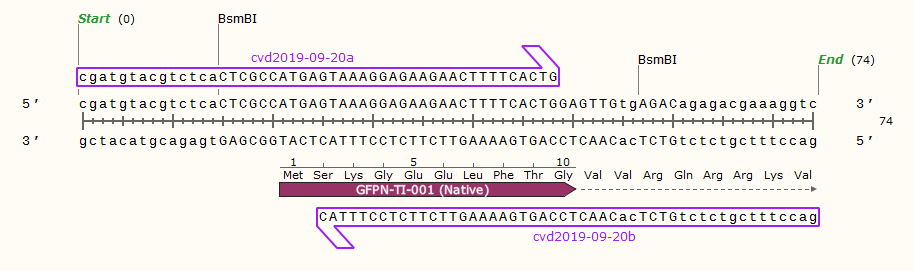
\includegraphics[width=1\textwidth]{appendix/TIsigner/Figs/S1.png}
	\caption[Strategy for producing a double stranded DNA corresponding to the first ten codons of each of the TIsigner variants of GFP.]{\textbf{Strategy for producing a double stranded DNA corresponding to the first ten codons of each of the TIsigner variants of GFP.} The strategy employs a pair of primers that overlap at their 3’ ends that, upon annealing together, can be used as a template for Q5 polymerase to generate a double stranded DNA spanning the N-terminal region of GFP (i.e. GFPN). Shown here is the sequence of variant GFPN-001 generated using the overlapping cvd2019-09-20a forward and cvd2019-09-20b reverse primer pair (see Table S2). The resultant double stranded DNA can then be cloned into the MIDAS pML1 vector by digestion with the Type IIS restriction enzyme BsmBI (recognition site CGTCTC(1/5)). The same primer pair strategy was used for producing TIsigner variants of luciferase, albeit with a different [AGGA] suffix. This map was created with SnapGene.
		
	}%the List of Figures because of the *}
	\label{fig:appendix_TIsigner_S1}
\end{figure}


\begin{figure}[htbp!]
	\center
	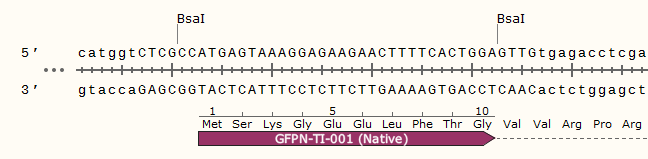
\includegraphics[width=1\textwidth]{appendix/TIsigner/Figs/S2.png}
	\caption[Structure of GFPN variants cloned into the pML1 vector.]{\textbf{Structure of GFPN variants cloned into the pML1 vector.} Following BsmBI-mediated cloning into the pML1 vector, each GFPN variant becomes flanked by BsaI recognition sites (GGTCTC(1/5)). BsaI cleaves at the CCAT prefix upstream of the GFPN sequence and at the GTTG suffix (downstream of the GFPN module). For ease of depiction, only the sequences immediately surrounding the cloned GFPN fragment are shown (i.e., not the rest of the pML1 vector). The structure of luciferase RLucN variants is identical, except for having a different [AGGA] suffix sequence.
		
	}%the List of Figures because of the *}
	\label{fig:appendix_TIsigner_S2}
\end{figure}



\begin{figure}[htbp!]
	\center
	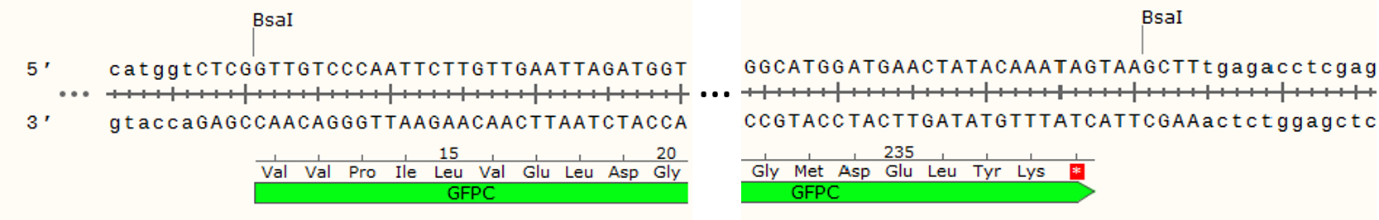
\includegraphics[width=1\textwidth]{appendix/TIsigner/Figs/S3.png}
	\caption[Structure of the GFPC fragment cloned into the pML1 vector.]{\textbf{Structure of the GFPC fragment cloned into the pML1 vector.} Following BsmBI-mediated cloning into the pML1 vector, GFPC becomes flanked by BsaI recognition sites. BsaI cleaves at the [GTTG] prefix (upstream of the GFPC sequence) and at the downstream [GCTT] suffix. For ease of depiction, only sequences around the 5’ and 3’ ends of the GFPC fragment are shown (left- and right-hand sides, respectively). In the case of luciferase, the prefix sequence is [AGGA].
	}%the List of Figures because of the *}
	\label{fig:appendix_TIsigner_S3}
\end{figure}

\begin{figure}[htbp!]
	\center
	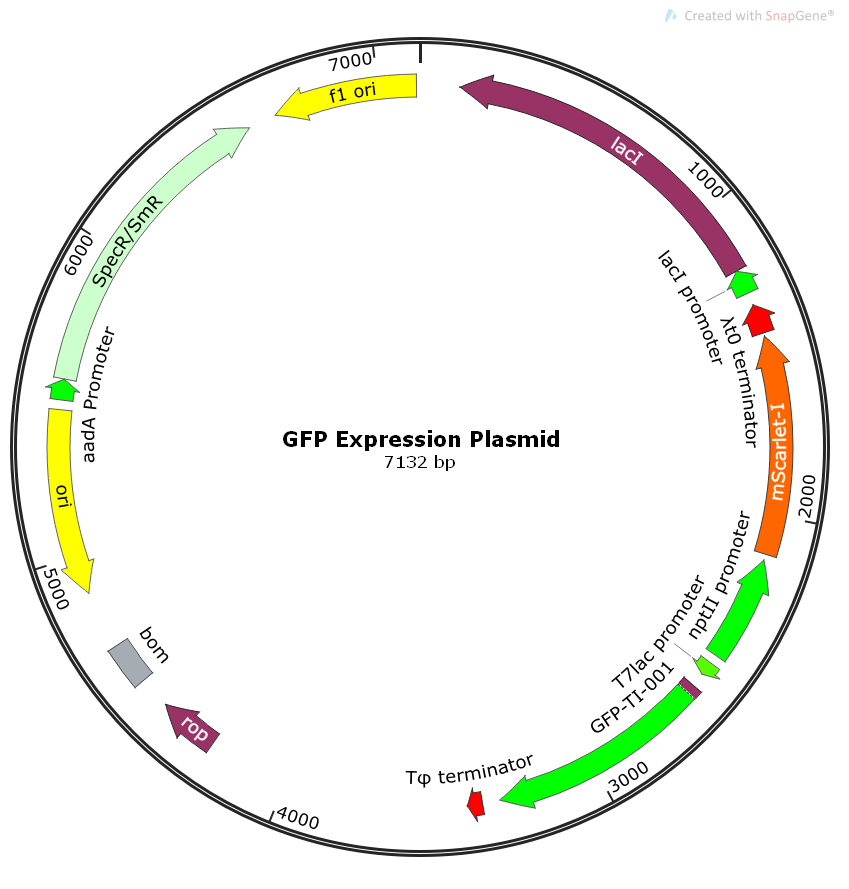
\includegraphics[width=1\textwidth]{appendix/TIsigner/Figs/S4.png}
	\caption[Structure of GFP expression plasmids.]{\textbf{Structure of GFP expression plasmids.} Map view showing the architecture of MIDAS-assembled plasmids used for expression of GFP TIsigner variants. Expression of each of the gfp variants is controlled by the T7lac promoter and oriented such that they are divergently transcribed with respect to the mScarlet-I device, which is driven by the nptII promoter. The devices for lacI, mScarlet-I and gfp were loaded sequentially into plasmid pML3.2, which has the medium copy replication origin from the pET series of vectors (ori-bom-rop) in place of the high copy pMB1 replicon in the pML3 destination vector described in van Dolleweerd et al, 2018 \cite{Van_Dolleweerd2018-pw}, and a selectable marker conferring resistance to spectinomycin.
		
	}%the List of Figures because of the *}
	\label{fig:appendix_TIsigner_S4}
\end{figure}

\begin{figure}[htbp!]
	\center
	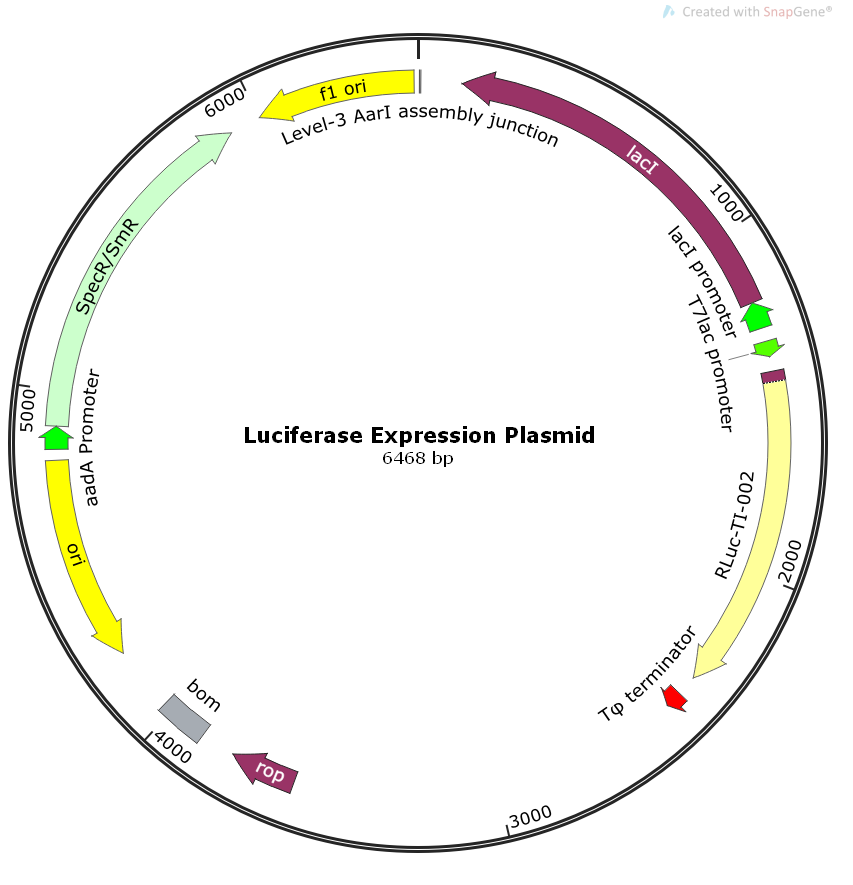
\includegraphics[width=1\textwidth]{appendix/TIsigner/Figs/S5.png}
	\caption[Structure of luciferase expression plasmids.]{\textbf{Structure of luciferase expression plasmids.} Map view showing the architecture of MIDAS-assembled plasmids used for expression of luciferase TIsigner variants. Expression of each of the luciferase variants is controlled by the T7lac promoter and oriented such that they are divergently transcribed with respect to the lacI device, which is driven by the lacI promoter. The devices for lacI and luciferase were loaded sequentially into plasmid pML3.2, which has the medium copy replication origin from the pET series of vectors (ori-bom-rop) in place of the high copy pMB1 replicon in the pML3 destination vector described in van Dolleweerd et al, 2018 \cite{Van_Dolleweerd2018-pw}, and a selectable marker conferring resistance to spectinomycin.
		
	}%the List of Figures because of the *}
	\label{fig:appendix_TIsigner_S5}
\end{figure}


\section{Supplementary figures}
\begin{figure}[htbp!]
	\center
	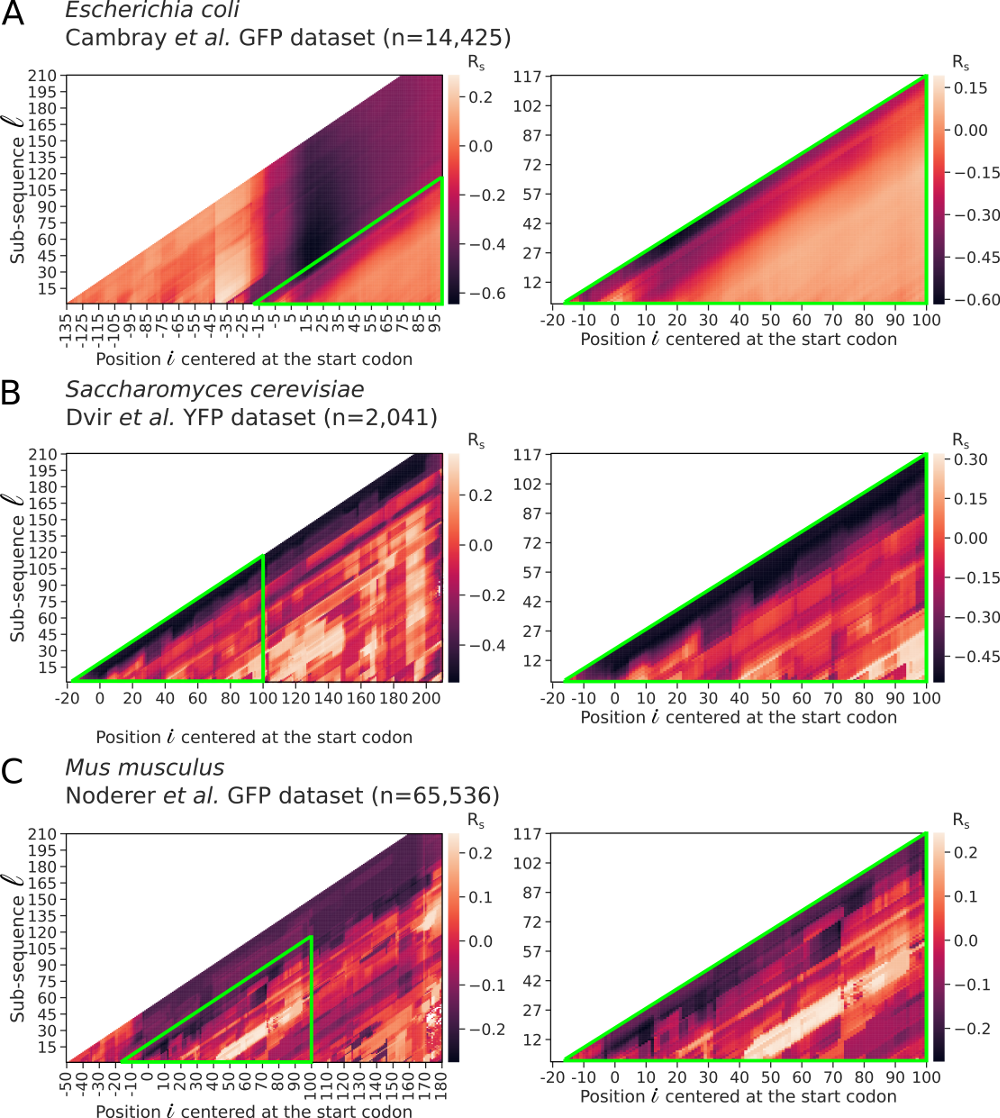
\includegraphics[width=1\textwidth]{appendix/TIsigner/Figs/S6.png}
	\caption[Heatmaps of correlations between opening energy and protein abundance for each of the sub-sequence regions (related to Fig 1).]{\textbf{Heatmaps of correlations between opening energy and protein abundance for each of the sub-sequence regions (related to Fig 1).} Green unfilled triangles indicate the regions before and after scaling (left and right panels, respectively). (A) For E. coli, we used a representative GFP expression dataset from Cambray et al. (2018) \cite{Cambray2018-kn}. The reporter library consists of GFP fused in-frame with a library of 96-nt upstream sequences (n=14,425). (B) For S. cerevisiae, we used a YFP expression dataset from Dvir et al. (2013) \cite{Dvir2013-zt}. The YFP reporter library consists of 2,041 random decameric nucleotides inserted at the upstream of YFP start codon. (C) For M. musculus, we used the GFP expression dataset from Noderer et al. (2014) \cite{Noderer2014-aq}. The GFP reporter library consists of 65,536 random hexameric and dimeric nucleotides inserted at the upstream and downstream of GFP start codon, respectively. $R_s$, Spearman’s rho.
	}%the List of Figures because of the *}
	\label{fig:appendix_TIsigner_S6}
\end{figure}

\begin{SCfigure}[][hbtp!]
	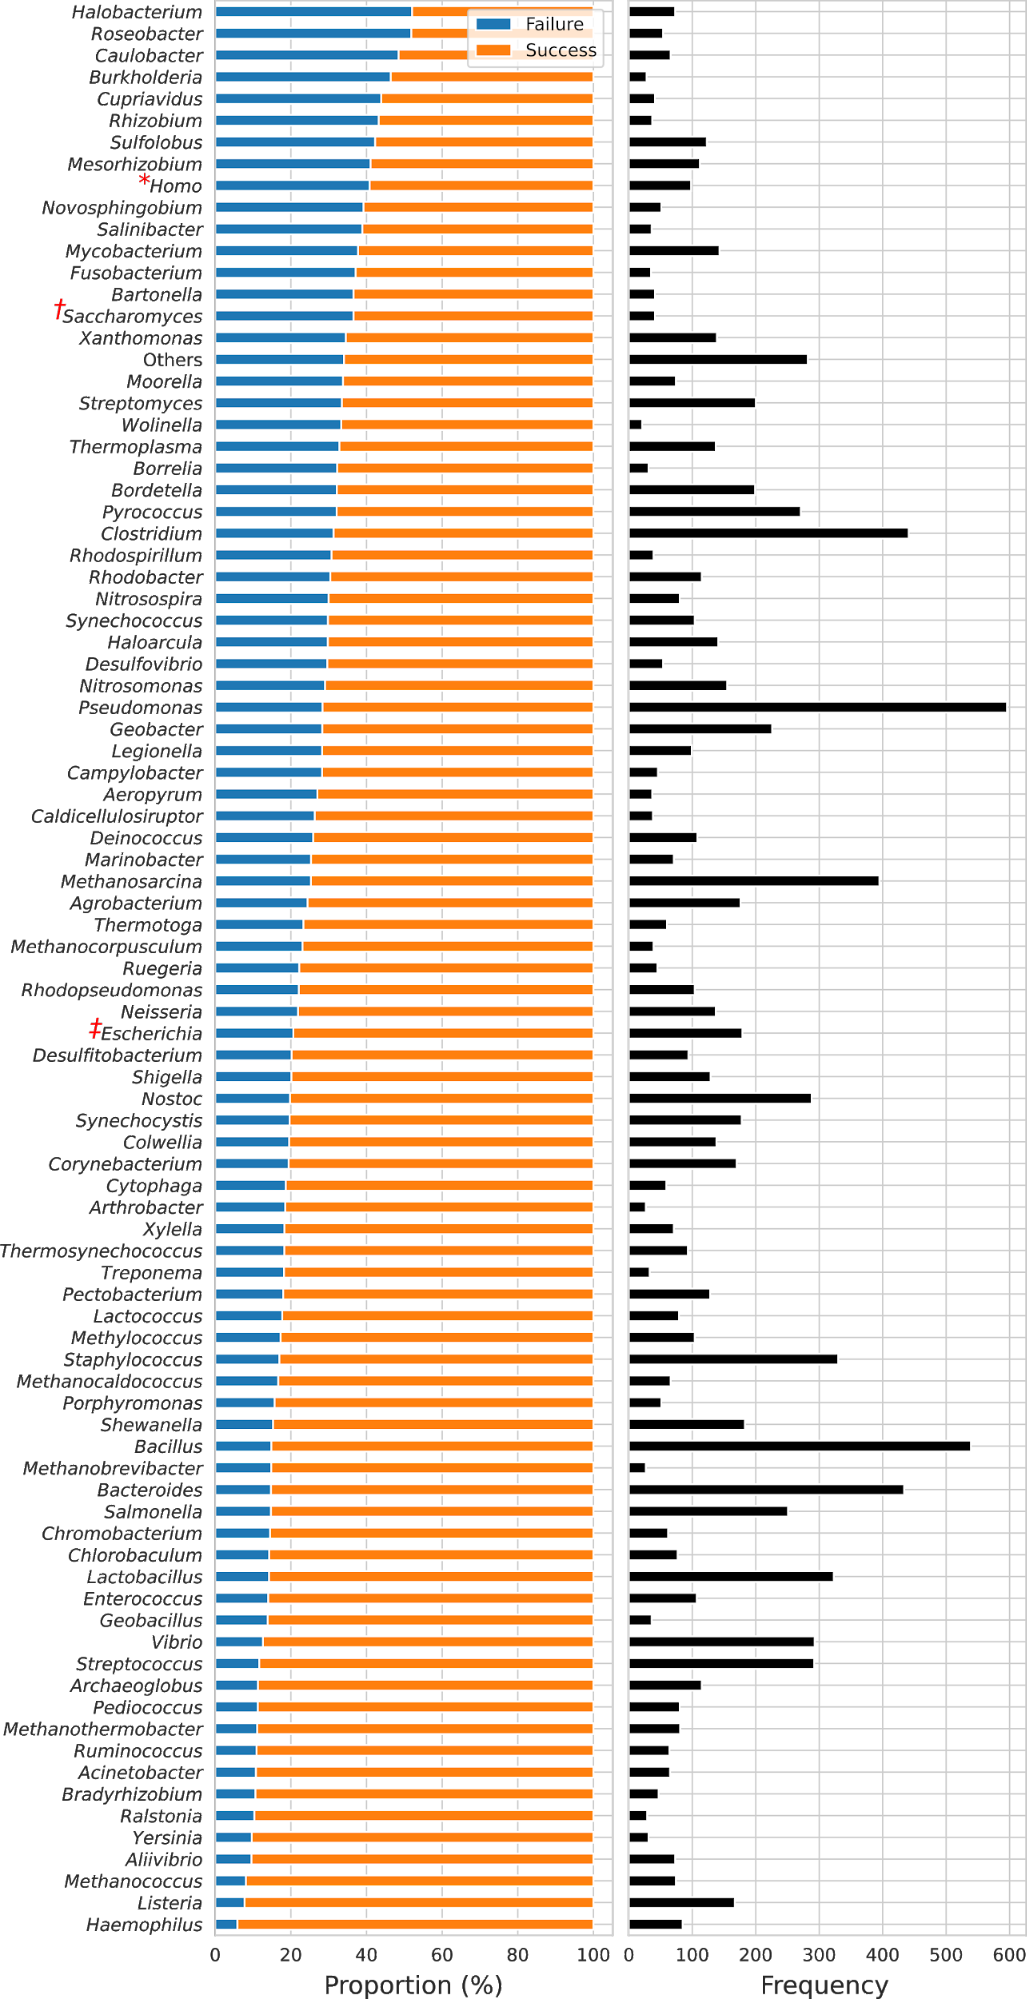
\includegraphics[width=0.5\textwidth]{appendix/TIsigner/Figs/S7.png}
	\caption[ Expression outcomes of the PSI:Biology targets in E. coli (related to Fig 2C and 3). ]{\textbf{ Expression outcomes of the PSI:Biology targets in \textit{E. coli} (related to Fig \ref{fig:tisigner_fig2}C and \ref{fig:tisigner_fig3}). } A total of 11,430 PSI:Biology targets from over 189 species were analysed in this study (n=8,780 and 2,650, ‘success’ and ‘failure’ groups, respectively) \cite{Chen2004-is,Seiler2014-ox,Acton2005-sr}. Genera with at least 20 target genes are shown and the remaining as ‘Others’. The top three PSI:Biology targets are from four Pseudomonas, five Bacillus and six Clostridium species. Red asterisk, obelisk and diesis indicate Homo sapiens, S. cerevisiae and E. coli, respectively. These target genes were inserted into the pET21\_NESG expression vector, in which the promoter and fusion tag are T7lac and C-terminal His tag, respectively.}
	\label{fig:appendix_TIsigner_S7}
\end{SCfigure}



\begin{figure}[htbp!]
	\center
	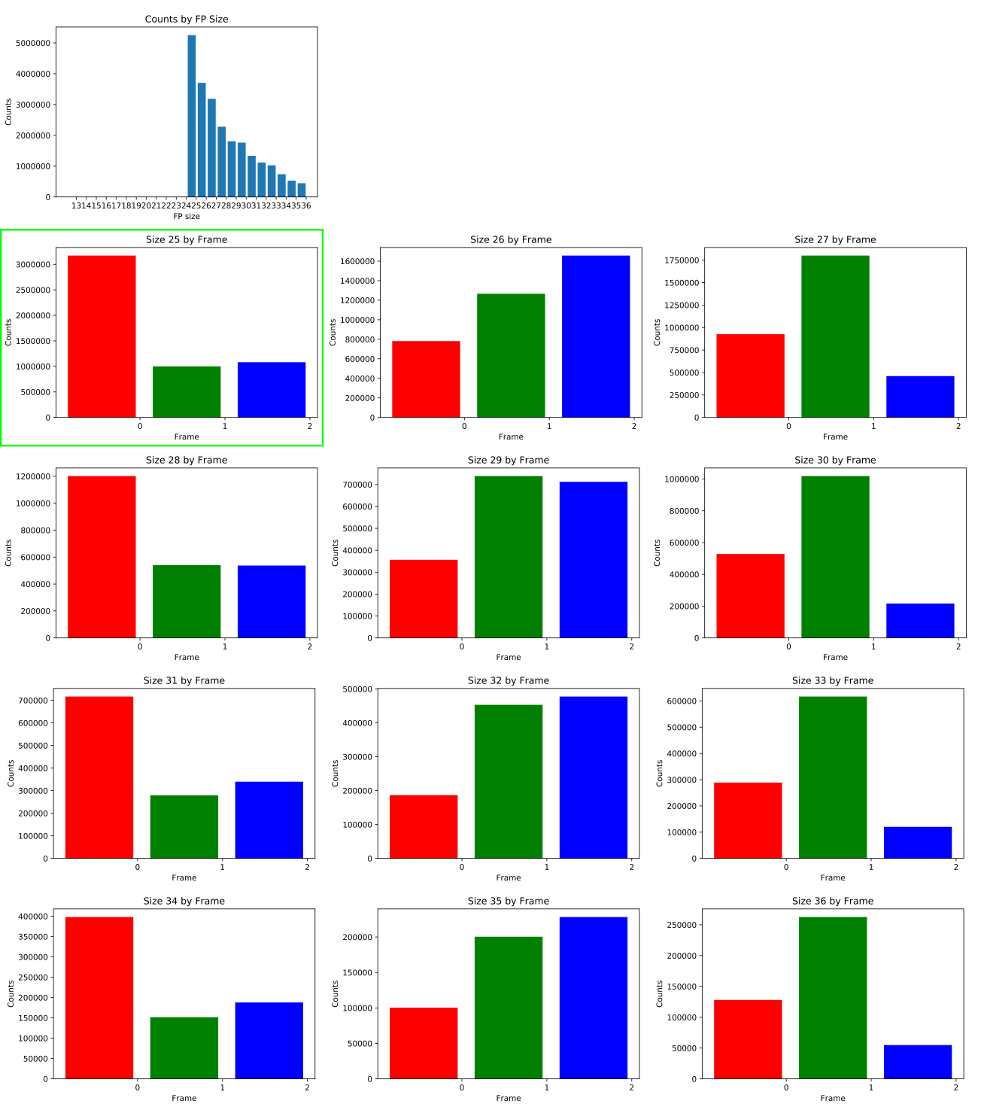
\includegraphics[width=1\textwidth]{appendix/TIsigner/Figs/S8.png}
	\caption[Ribosome footprints in 25-nt fragments show a strong triplet periodicity, indicating translation (related to Fig \ref{fig:tisigner_fig3})]{\textbf{Ribosome footprints in 25-nt fragments show a strong triplet periodicity, indicating translation (related to Fig \ref{fig:tisigner_fig3})}  These 25-nt footprints (green unfilled rectangle) were used to train a neural network model \cite{Tunney2018-kk} in order to predict the translation elongation rates of the PSI:Biology targets. Ribosome profiling data [SRR7759806 and SRR7759807 \cite{Mohammad2019-if}] were first aligned to S. cerevisiae transcriptome. SAM alignment files were merged, and ribosome footprints which were mapped to each frame were enumerated. See https://github.com/Gardner-BinfLab/TIsigner\_paper\_2019. FP, footprints. 
	}%the List of Figures because of the *}
	\label{fig:appendix_TIsigner_S8}
\end{figure}

\begin{figure}[htbp!]
	\center
	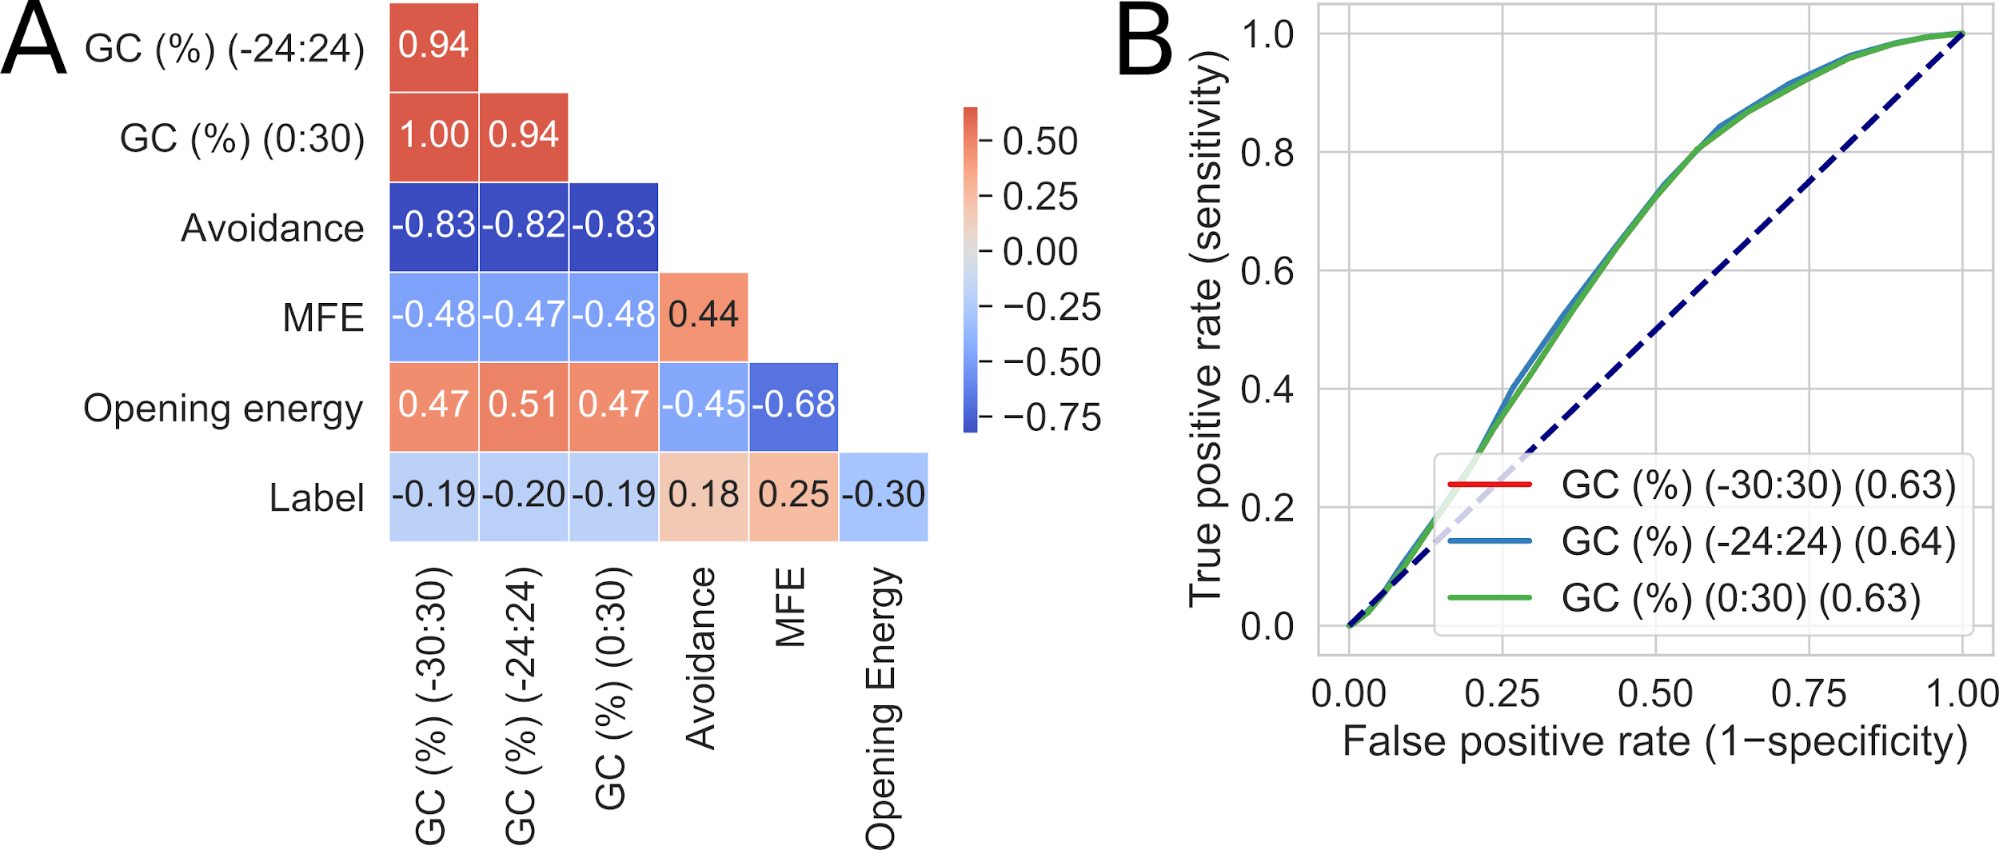
\includegraphics[width=1\textwidth]{appendix/TIsigner/Figs/S9.png}
	\caption[Analysis of the local G+C contents in the PSI:Biology target genes (related to Fig \ref{fig:tisigner_fig3}).]{\textbf{Analysis of the local G+C contents in the PSI:Biology target genes (related to Fig \ref{fig:tisigner_fig3}). (A) }  The G+C contents in the regions −24:24 and −30:30 weakly correlate with opening energy and minimum free energy, respectively. Green unfilled squares indicate Spearman’s correlations ($R_s$) between the local G+C contents and the corresponding local features. \textbf{B}  The local G+C contents show a similar prediction accuracy (AUC scores shown in parentheses).
	}%the List of Figures because of the *}
	\label{fig:appendix_TIsigner_S9}
\end{figure}



\begin{SCfigure}[][hbtp!]
	\includegraphics[width=0.5\textwidth]{appendix/TIsigner/Figs/S10.png}
	\caption[Accessibility of translation initiation sites can be increased by synonymous codon substitution within the first nine codons using simulated annealing.]{\textbf{Accessibility of translation initiation sites can be increased by synonymous codon substitution within the first nine codons using simulated annealing. (A)} Schedules in simulated annealing. The ratio of temperature to the number of the first N substitutable codons decreases exponentially with increasing number of iterations. \textbf{(B)} Accessibility of translation initiation sites increases with increasing number of the first N replaceable codons. The PSI:Biology targets that failed to be expressed were optimised using simulated annealing (n=2,650). The Kolmogorov-Smirnov distance between the distributions of ‘9’ and ‘full-length’ was significantly different but sufficiently close (DKS=0.09, P<10-7), indicating that optimisation of the first nine codons can achieve nearly optimum accessibility. For comparison, the distribution of the PSI:Biology targets that were successfully expressed are shown (n=8,780). See also Table S4. \textbf{(C)} Accessibility of translation initiation sites can be increased indirectly using the existing gene optimisation tools and random synonymous codon substitution. ‘TIsigner (9)’ refers to the default settings of our tool, which allows synonymous substitutions up to the first nine codons (as above). See also Table S4. \textbf{(D)} Accessibility of translation initiation sites can be optimised using PCR cloning. The forward primer should be designed according to TIsiger optimised sequences. For example, using a nested PCR approach, the optimised sequence can be produced using the forward primer designed with appropriate mismatches (gold bulges) to amplify the amplicon from the initial PCR reaction.
	}
	\label{fig:appendix_TIsigner_S10}
\end{SCfigure}


\begin{figure}[htbp!]
	\center
	\includegraphics[width=0.5\textwidth]{appendix/TIsigner/Figs/S11.png}
	\caption[Sequence length does not affect software performance because only a fixed region is taken into account during optimisation ($\mathcal{O}(1)$ time). ]{\protect\rule{0ex}{5ex}\textbf{Sequence length does not affect software performance because only a fixed region is taken into account during optimisation ($\mathcal{O}(1)$ time). } 
	}
	\label{fig:appendix_TIsigner_S11}
\end{figure}

\begin{SCfigure}[][hbtp!]
	\includegraphics[width=0.5\textwidth]{appendix/TIsigner/Figs/S12.png}
	\caption[Opening energy of 10 or below at the region −24:24 is about two times more likely to come from the target genes that are successfully expressed than those that failed (related to Fig \ref{fig:tisigner_fig3}). ]{\textbf{Opening energy of 10 or below at the region −24:24 is about two times more likely to come from the target genes that are successfully expressed than those that failed (related to Fig \ref{fig:tisigner_fig3}).} Cumulative frequency distributions of the true positive and false positive (less than type), and true negative and false negative (more than type) derived from the ROC analysis in Fig \ref{fig:tisigner_fig3}B (left panel, opening energy −24:24). These values were used to estimate positive likelihood ratios with 95\% confidence intervals using 10,000 bootstrap replicates. The estimated ratios and/or confidence intervals are inaccurate at low numbers of true positives or true negatives. Therefore, a four-parameter logistic curve was fitted to the positive likelihood ratios. Fitted values are useful to estimate the posterior probability of protein expression.

	}
	\label{fig:appendix_TIsigner_S12}
\end{SCfigure}

\clearpage

\section{Supplementary tables}


% Please add the following required packages to your document preamble:
% \usepackage{longtable}
% Note: It may be necessary to compile the document several times to get a multi-page table to line up properly
\begin{longtable}{|l|l|}
	\caption{MIDAS parts used in this work. The sequence of each part is shown, with BsmBI recognition sites used for cloning into the MIDAS pML1 vector underlined. MIDAS prefix and suffix nucleotides are highlighted by the bold blue and red text, respectively. The T7lac promoter and T7 Tφ transcription terminator (both sequences taken from pET-15b) were ordered as double-stranded DNA gBlocks from IDT. The lacI genetic element (with lacI promoter in green and lacI coding sequence in blue) was from GeneArt. Other parts were amplified by polymerase chain reaction. For the mScarlet-I part, the coding sequence is highlighted by the blue shading. Sequences of all parts were confirmed following cloning into the MIDAS pML1 vector.
	}
	\label{tab:appendix_TIsigner_T2}\\
	\hline
	\textbf{Part} &
	\textbf{Sequence} \\ \hline
	\endhead
	%
	T7lac promoter &
	\begin{tabular}[c]{@{}l@{}}cgatgtacgtctcaCTCGGGAGCGATCCCGCGAAATTAATACGACT\\ CACTATAGGGGAATTGTGAGCGGATAACAATTCCCCTCTAGAA\\ ATAATTTTGTTTAACTTTAAGAAGGAGATATACCATtgAGACag\\ agacgaaaggtc\end{tabular} \\ \hline
	nptII promoter &
	\begin{tabular}[c]{@{}l@{}}cgatgtacgtctcaCTCGGGAGctcgcacgctgccgcaagcactcagggcg\\ caagggctgctaaaggaagcggaacacgtagaaagccagtccgcagaaacgg\\ tgctgaccccggatgaatgtcagctactgggctatctggacaagggaaaacgca\\ agcgcaaagagaaagcaggtagcttgcagtgggcttacatggcgatagctaga\\ ctgggcggtcttatggacagcaagcgaaccggaattgccagctggggcgccct\\ ctggtaaggttgggaagccctgcaaagtaaactggatggctttcttgccgccaag\\ gatctgatggcgcaggggatcaagatctgatcaagagacaggatactagtggag\\ gaagaaaaAATGtgAGACagagacgaaaggtc\end{tabular} \\ \hline
	lacI genetic element &
	\begin{tabular}[c]{@{}l@{}}cgatgtacgtctcaCTCGGGAGCGTCGAGATCCCG\hlc[green]{GACACCATCG}\\ \hlc[green]{AATGGCGCAAAACCTTTCGCGGTATGGCATGATAGCGCCCGG}\\ \hlc[green]{AAGAGAGTCAATTCAGGGTGGTGAAT}\hlc[blue]{GTGAAACCAGTAACGT}\\ \hlc[blue]{TATACGATGTCGCAGAGTATGCCGGTGTCTCTTATCAGACCGT}\\ \hlc[blue]{TTCCCGCGTGGTGAACCAGGCCAGCCACGTTTCTGCGAAAA}\\ \hlc[blue]{CGCGGGAAAAAGTGGAAGCGGCGATGGCGGAGCTGAATTAC}\\ \hlc[blue]{ATTCCCAACCGCGTGGCACAACAACTGGCGGGCAAACAGTC}\\ \hlc[blue]{GTTGCTGATTGGCGTTGCCACCTCCAGTCTGGCCCTGCACG}\\ \hlc[blue]{CGCCGTCGCAAATTGTCGCGGCGATTAAATCTCGCGCCGAT}\\ \hlc[blue]{CAACTGGGTGCCAGCGTGGTGGTGTCGATGGTAGAACGAAG}\\ \hlc[blue]{CGGCGTCGAAGCCTGTAAAGCGGCGGTGCACAATCTTCTCG}\\ \hlc[blue]{CGCAACGCGTCAGTGGGCTGATCATTAACTATCCGCTGGATG}\\ \hlc[blue]{ACCAGGATGCCATTGCTGTGGAAGCTGCCTGCACTAATGTTC}\\ \hlc[blue]{CGGCGTTATTTCTTGATGTCTCTGACCAGACACCCATCAACA}\\ \hlc[blue]{GTATTATTTTCTCCCATGAAGACGGTACGCGACTGGGCGTGG}\\ \hlc[blue]{AGCATCTGGTCGCATTGGGTCACCAGCAAATCGCGCTGTTAG}\\ \hlc[blue]{CGGGCCCATTAAGTTCTGTCTCGGCGCGTCTGCGTCTGGCT}\\ \hlc[blue]{GGCTGGCATAAATATCTCACTCGCAATCAAATTCAGCCGATAG}\\ \hlc[blue]{CGGAACGGGAAGGCGACTGGAGTGCCATGTCCGGTTTTCAA}\\ \hlc[blue]{CAAACCATGCAAATGCTGAATGAGGGCATCGTTCCCACTGCG}\\ \hlc[blue]{ATGCTGGTTGCCAACGATCAGATGGCGCTGGGCGCAATGCG}\\ \hlc[blue]{CGCCATTACCGAGTCCGGGCTGCGCGTTGGTGCGGATATCTC}\\ \hlc[blue]{GGTAGTGGGATACGACGATACCGAAGACAGCTCATGTTATATC}\\ \hlc[blue]{CCGCCGTTAACCACCATCAAACAGGATTTTCGCCTGCTGGGG}\\ \hlc[blue]{CAAACCAGCGTGGACCGCTTGCTGCAACTCTCTCAGGGCCA}\\ \hlc[blue]{GGCGGTGAAGGGCAATCAGCTGTTGCCCGTGTCACTGGTGAA}\\ \hlc[blue]{AAGAAAAACCACCCTGGCGCCCAATACGCAAACCGCCTCTCC}\\ \hlc[blue]{CCGCGCGTTGGCCGATTCATTAATGCAGCTGGCACGACAGGT}\\ \hlc[blue]{TTCCCGACTGGAAAGCGGGCAGTGA}GCGCAACGCAATTAATG\\ TAAGTTAGCTCACTCATTAGGCACCGGGATCTCGACCGATGCC\\ CTTGAGAGCCTTCAACCCAGTCAGCTCCTTCCGGTGGGCGCG\\ GGGCATGACTACGCTtgAGACagagacgaaaggtc\end{tabular} \\ \hline
	mScarlet-I coding sequence (CDS) &
	\begin{tabular}[c]{@{}l@{}}cgatgtacgtctcaCTCGA\hlc[blue]{ATGgtgagcaagggcgaggcagtgatcaaggag}\\ \hlc[blue]{ttcatgcggttcaaggtgcacatggagggctccatgaacggccacgagttcgagat}\\ \hlc[blue]{cgagggcgagggcgagggccgcccctacgagggcacccagaccgccaagctga}\\ \hlc[blue]{aggtgaccaagggtggccccctgcccttctcctgggacatcctgtcccctcagttca}\\ \hlc[blue]{tgtacggctccagggccttcatcaagcaccccgccgacatccccgactactataag}\\ \hlc[blue]{cagtccttccccgagggcttcaagtgggagcgcgtgatgaacttcgaggacggcg}\\ \hlc[blue]{gcgccgtgaccgtgacccaggacacctccctggaggacggcaccctgatctacaa}\\ \hlc[blue]{ggtgaagctccgcggcaccaacttccctcctgacggccccgtaatgcagaagaag}\\ \hlc[blue]{acaatgggctgggaagcgtccaccgagcggttgtaccccgaggacggcgtgctg}\\ \hlc[blue]{aagggcgacattaagatggccctgcgcctgaaggacggcggccgctacctggcg}\\ \hlc[blue]{gacttcaagaccacctacaaggccaagaagcccgtgcagatgcccggcgcctaca}\\ \hlc[blue]{acgtcgaccgcaagttggacatcacctcccacaacgaggactacaccgtggtgga}\\ \hlc[blue]{acagtacgaacgctccgagggccgccactccaccggcggcatggacgagctgta}\\ \hlc[blue]{caagtaa}GCTTtgAGACagagacgaaaggtc\end{tabular} \\ \hline
	Phage T7 T$\phi$ transcription terminator &
	\begin{tabular}[c]{@{}l@{}}cgatgtacgtctcaCTCGGCTTCAAAGCCCGAAAGGAAGCTGAGTT\\ GGCTGCTGCCACCGCTGAGCAATAACTAGCATAACCCCTTGG\\ GGCCTCTAAACGGGTCTTGAGGGGTTTTTTGCTGAAAGGAGG\\ AACTATATCCGGATCGCTtgAGACagagacgaaaggtc\end{tabular} \\ \hline
	Lambda t0 transcription terminator &
	\begin{tabular}[c]{@{}l@{}}cgatgtacgtctcaCTCGGCTTggactcctgttgatagatccagtaatgacctc\\ agaactccatctggatttgttcagaacgctcggttgccgccgggcgttttttattggt\\ gagaatccaagctagcttggCGCTtgAGACagagacgaaaggtc\end{tabular} \\ \hline
\end{longtable}




\begin{landscape}
	\begin{longtable}{|l|l|l|}
		\caption[Oligonucleotide primer pairs for constructing TIsigner variants of gfp. ]{Oligonucleotide primer pairs for constructing TIsigner variants of gfp. The sequences of each forward and reverse primer pair used for constructing each of the gfp TIsigner variants is shown. The start codon in each of the forward primers is shaded yellow. BsmBI recognition sites (used for Golden Gate assembly into the MIDAS pML1 vector) are underlined.}
%		 The MIDAS prefix [CCAT] and suffix [GTTG] (reverse-complement = CAAC) for the GFPN modules are highlighted in bold blue and red, respectively.}
		\label{tab:appendix_TIsigner_T2}\\
		\hline
		\textbf{\textbf{GFPN TIsigner ID}} & \textbf{Oligonucleotide Primer Pair} & \textbf{Primer Sequences (5’ to 3’)} \\ \hline
		\endfirsthead
		%
		\multicolumn{3}{c}%
		{{\bfseries Table \thetable\ continued from previous page}} \\
		\hline
		\textbf{\textbf{GFPN TIsigner ID}} & \textbf{Oligonucleotide Primer Pair} & \textbf{Primer Sequences (5’ to 3’)} \\ \hline
		\endhead
		%
		\multirow{2}{*}{GFPN-001} & cvd2019-09-20a & \underline{cgatgtacgtctc}aCTCGCCATGAGTAAAGGAGAAGAACTTTTCACTG   \\ \cline{2-3} 
		& cvd2019-09-20b & \underline{gacctttcgtctc}tGTCTcaCAACTCCAGTGAAAAGTTCTTCTCCTTTAC \\ \hline
		\multirow{2}{*}{GFPN-002} & cvd2019-09-21a & \underline{cgatgtacgtctc}aCTCGCCATGTCGAAGGGTGAAGAACTCTTCAC     \\ \cline{2-3} 
		& cvd2019-09-21b & \underline{gacctttcgtctc}tGTCTcaCAACACCAGTGAAGAGTTCTTCACCCTTC  \\ \hline
		\multirow{2}{*}{GFPN-003} & cvd2019-09-21c & \underline{cgatgtacgtctc}aCTCGCCATGAGTAAAGGGGAGGAACTCTTTAC     \\ \cline{2-3} 
		& cvd2019-09-21d & \underline{gacctttcgtctc}tGTCTcaCAACCCCGGTAAAGAGTTCCTCCCCTTTAC \\ \hline
		\multirow{2}{*}{GFPN-004} & cvd2019-09-21e & \underline{cgatgtacgtctc}aCTCGCCATGTCGAAGGGCGAAGAACTCTTC       \\ \cline{2-3} 
		& cvd2019-09-21f & \underline{gacctttcgtctc}tGTCTcaCAACACCAGTGAAGAGTTCTTCGCCCTTC  \\ \hline
		\multirow{2}{*}{GFPN-005} & cvd2019-09-21g & \underline{cgatgtacgtctc}aCTCGCCATGTCTAAGGGTGAGGAGCTCTTC       \\ \cline{2-3} 
		& cvd2019-09-21h & \underline{gacctttcgtctc}tGTCTcaCAACTCCCGTGAAGAGCTCCTCACCCTTAG \\ \hline
		\multirow{2}{*}{GFPN-006} & cvd2019-09-21i & \underline{cgatgtacgtctc}aCTCGCCATGTCGAAAGGGGAAGAACTGTTCAC     \\ \cline{2-3} 
		& cvd2019-09-21j & \underline{gacctttcgtctc}tGTCTcaCAACGCCGGTGAACAGTTCTTCCCCTTTC  \\ \hline
		\multirow{2}{*}{GFPN-007} & cvd2019-09-21k & \underline{cgatgtacgtctc}aCTCGCCATGTCTAAAGGAGAAGAGCTTTTCAC     \\ \cline{2-3} 
		& cvd2019-09-21l & \underline{gacctttcgtctc}tGTCTcaCAACCCCAGTGAAAAGCTCTTCTCCTTTAG \\ \hline
		\multirow{2}{*}{GFPN-008} & cvd2019-09-21m & \underline{cgatgtacgtctc}aCTCGCCATGAGTAAGGGTGAGGAATTATTCACG    \\ \cline{2-3} 
		& cvd2019-09-21n & \underline{gacctttcgtctc}tGTCTcaCAACGCCCGTGAATAATTCCTCACCCTTAC \\ \hline
		\multirow{2}{*}{GFPN-009} & cvd2019-09-22a & \underline{cgatgtacgtctc}aCTCGCCATGAGTAAAGGGGAAGAACTGTTCAC     \\ \cline{2-3} 
		& cvd2019-09-22b & \underline{gacctttcgtctc}tGTCTcaCAACGCCAGTGAACAGTTCTTCCCCTTTAC \\ \hline
		\multirow{2}{*}{GFPN-010} & cvd2019-09-22c & \underline{cgatgtacgtctc}aCTCGCCATGTCTAAGGGTGAGGAGCTCTTC       \\ \cline{2-3} 
		& cvd2019-09-22d & \underline{gacctttcgtctc}tGTCTcaCAACTCCTGTGAAGAGCTCCTCACCCTTAG \\ \hline
		\multirow{2}{*}{GFPN-011} & cvd2019-09-22e & \underline{cgatgtacgtctc}aCTCGCCATGAGTAAAGGAGAAGAGTTATTTACTGG  \\ \cline{2-3} 
		& cvd2019-09-22f & \underline{gacctttcgtctc}tGTCTcaCAACTCCAGTAAATAACTCTTCTCCTTTAC \\ \hline
		\multirow{2}{*}{GFPN-012} & cvd2019-09-22g & \underline{cgatgtacgtctc}aCTCGCCATGAGTAAGGGAGAAGAGCTGTTC       \\ \cline{2-3} 
		& cvd2019-09-22h & \underline{gacctttcgtctc}tGTCTcaCAACTCCAGTGAACAGCTCTTCTCCCTTAC \\ \hline
		\multirow{2}{*}{GFPN-013} & cvd2019-09-22i & \underline{cgatgtacgtctc}aCTCGCCATGTCGAAAGGAGAAGAATTGTTCAC     \\ \cline{2-3} 
		& cvd2019-09-22j & \underline{gacctttcgtctc}tGTCTcaCAACGCCCGTGAACAATTCTTCTCCTTTCG \\ \hline
		\multirow{2}{*}{GFPN-014} & cvd2019-09-22k & \underline{cgatgtacgtctc}aCTCGCCATGAGCAAAGGAGAAGAATTATTTACTGG  \\ \cline{2-3} 
		& cvd2019-09-22l & \underline{gacctttcgtctc}tGTCTcaCAACTCCAGTAAATAATTCTTCTCCTTTGC \\ \hline
		\multirow{2}{*}{GFPN-015} & cvd2019-09-22m & \underline{cgatgtacgtctc}aCTCGCCATGAGCAAAGGAGAAGAATTATTTACGG   \\ \cline{2-3} 
		& cvd2019-09-22n & \underline{gacctttcgtctc}tGTCTcaCAACTCCCGTAAATAATTCTTCTCCTTTGC \\ \hline
		\multirow{2}{*}{GFPN-016} & cvd2019-09-22o & \underline{cgatgtacgtctc}aCTCGCCATGAGCAAAGGGGAAGAATTATTTACAG   \\ \cline{2-3} 
		& cvd2019-09-22p & \underline{gacctttcgtctc}tGTCTcaCAACACCTGTAAATAATTCTTCCCCTTTGC \\ \hline
		\multirow{2}{*}{GFPN-017} & cvd2020-03-05a & \underline{cgatgtacgtctc}aCTCGCCATGAGTAAAGGGGAAGAACTCTTTACC    \\ \cline{2-3} 
		& cvd2020-03-05b & \underline{gacctttcgtctc}tGTCTcaCAACCCCGGTAAAGAGTTCTTCCCCTTTAC \\ \hline
		\multirow{2}{*}{GFPN-018} & cvd2020-03-05c & \underline{cgatgtacgtctc}aCTCGCCATGTCGAAAGGTGAGGAACTATTCACTG   \\ \cline{2-3} 
		& cvd2020-03-05d & \underline{gacctttcgtctc}tGTCTcaCAACACCAGTGAATAGTTCCTCACCTTTC  \\ \hline
		\multirow{2}{*}{GFPN-019} & cvd2020-03-05e & \underline{cgatgtacgtctc}aCTCGCCATGTCGAAGGGTGAAGAACTGTTCACTG   \\ \cline{2-3} 
		& cvd2020-03-05f & \underline{gacctttcgtctc}tGTCTcaCAACACCAGTGAACAGTTCTTCACCCTTC  \\ \hline
		\multirow{2}{*}{GFPN-020} & cvd2020-03-05g & \underline{cgatgtacgtctc}aCTCGCCATGTCGAAGGGTGAAGAACTTTTCACTG   \\ \cline{2-3} 
		& cvd2020-03-05h & \underline{gacctttcgtctc}tGTCTcaCAACCCCAGTGAAAAGTTCTTCACCCTTC  \\ \hline
		\multirow{2}{*}{GFPN-021} & cvd2020-03-05i & \underline{cgatgtacgtctc}aCTCGCCATGTCCAAAGGGGAGGAACTCTTTACG    \\ \cline{2-3} 
		& cvd2020-03-05j & \underline{gacctttcgtctc}tGTCTcaCAACGCCCGTAAAGAGTTCCTCCCCTTTG  \\ \hline
		\multirow{2}{*}{GFPN-022} & cvd2020-03-05k & \underline{cgatgtacgtctc}aCTCGCCATGTCCAAAGGTGAAGAGCTTTTCACC    \\ \cline{2-3} 
		& cvd2020-03-05l & \underline{gacctttcgtctc}tGTCTcaCAACCCCGGTGAAAAGCTCTTCACCTTTG  \\ \hline
		\multirow{2}{*}{GFPN-023} & cvd2020-03-05m & \underline{cgatgtacgtctc}aCTCGCCATGTCGAAAGGTGAAGAGCTGTTCAC     \\ \cline{2-3} 
		& cvd2020-03-05n & \underline{gacctttcgtctc}tGTCTcaCAACACCGGTGAACAGCTCTTCACCTTTC  \\ \hline
		\multirow{2}{*}{GFPN-024} & cvd2020-03-05o & \underline{cgatgtacgtctc}aCTCGCCATGTCGAAAGGTGAGGAACTGTTCAC     \\ \cline{2-3} 
		& cvd2020-03-05p & \underline{gacctttcgtctc}tGTCTcaCAACCCCAGTGAACAGTTCCTCACCTTTC  \\ \hline
		\multirow{2}{*}{GFPN-025} & cvd2020-03-05q & \underline{cgatgtacgtctc}aCTCGCCATGAGTAAGGGGGAGGAGCTCTTCAC     \\ \cline{2-3} 
		& cvd2020-03-05r & \underline{gacctttcgtctc}tGTCTcaCAACTCCGGTGAAGAGCTCCTCCCCCTTAC \\ \hline
		\multirow{2}{*}{GFPN-026} & cvd2020-03-05s & \underline{cgatgtacgtctc}aCTCGCCATGAGTAAAGGGGAAGAGCTTTTCAC     \\ \cline{2-3} 
		& cvd2020-03-05t & \underline{gacctttcgtctc}tGTCTcaCAACCCCGGTGAAAAGCTCTTCCCCTTTAC \\ \hline
		\multirow{2}{*}{GFPN-027} & cvd2020-03-06a & \underline{cgatgtacgtctc}aCTCGCCATGAGTAAAGGAGAAGAACTCTTTACCG   \\ \cline{2-3} 
		& cvd2020-03-06b & \underline{gacctttcgtctc}tGTCTcaCAACTCCGGTAAAGAGTTCTTCTCCTTTAC \\ \hline
		\multirow{2}{*}{GFPN-028} & cvd2020-03-06c & \underline{cgatgtacgtctc}aCTCGCCATGAGTAAAGGAGAAGAACTCTTCACC    \\ \cline{2-3} 
		& cvd2020-03-06d & \underline{gacctttcgtctc}tGTCTcaCAACACCGGTGAAGAGTTCTTCTCCTTTAC \\ \hline
		\multirow{2}{*}{GFPN-029} & cvd2020-03-06e & \underline{cgatgtacgtctc}aCTCGCCATGTCAAAGGGGGAAGAACTGTTCAC     \\ \cline{2-3} 
		& cvd2020-03-06f & \underline{gacctttcgtctc}tGTCTcaCAACGCCTGTGAACAGTTCTTCCCCCTTTG \\ \hline
		\multirow{2}{*}{GFPN-030} & cvd2020-03-06g & \underline{cgatgtacgtctc}aCTCGCCATGTCGAAAGGCGAGGAACTGTTCAC     \\ \cline{2-3} 
		& cvd2020-03-06h & \underline{gacctttcgtctc}tGTCTcaCAACTCCAGTGAACAGTTCCTCGCCTTTC  \\ \hline
		\multirow{2}{*}{GFPN-031} & cvd2020-03-06i & \underline{cgatgtacgtctc}aCTCGCCATGAGCAAGGGTGAAGAGTTATTCACTG   \\ \cline{2-3} 
		& cvd2020-03-06j & \underline{gacctttcgtctc}tGTCTcaCAACTCCAGTGAATAACTCTTCACCCTTG  \\ \hline
		\multirow{2}{*}{GFPN-032} & cvd2020-03-06k & \underline{cgatgtacgtctc}aCTCGCCATGTCTAAAGGTGAAGAACTATTCACAGG  \\ \cline{2-3} 
		& cvd2020-03-06l & \underline{gacctttcgtctc}tGTCTcaCAACCCCTGTGAATAGTTCTTCACCTTTAG \\ \hline
		\multirow{2}{*}{GFPN-033} & cvd2020-03-06m & \underline{cgatgtacgtctc}aCTCGCCATGTCTAAAGGTGAGGAGCTCTTCAC     \\ \cline{2-3} 
		& cvd2020-03-06n & \underline{gacctttcgtctc}tGTCTcaCAACTCCTGTGAAGAGCTCCTCACCTTTAG \\ \hline
		\multirow{2}{*}{GFPN-034} & cvd2020-03-06o & \underline{cgatgtacgtctc}aCTCGCCATGAGTAAGGGAGAGGAACTGTTCAC     \\ \cline{2-3} 
		& cvd2020-03-06p & \underline{gacctttcgtctc}tGTCTcaCAACCCCTGTGAACAGTTCCTCTCCCTTAC \\ \hline
		\multirow{2}{*}{GFPN-035} & cvd2020-03-06q & \underline{cgatgtacgtctc}aCTCGCCATGTCGAAAGGGGAAGAATTGTTCAC     \\ \cline{2-3} 
		& cvd2020-03-06r & \underline{gacctttcgtctc}tGTCTcaCAACTCCAGTGAACAATTCTTCCCCTTTCG \\ \hline
		\multirow{2}{*}{GFPN-036} & cvd2020-03-06s & \underline{cgatgtacgtctc}aCTCGCCATGAGTAAGGGGGAGGAGCTGTTC       \\ \cline{2-3} 
		& cvd2020-03-06t & \underline{gacctttcgtctc}tGTCTcaCAACTCCTGTGAACAGCTCCTCCCCCTTAC \\ \hline
		\multirow{2}{*}{GFPN-037} & cvd2020-03-07a & \underline{cgatgtacgtctc}aCTCGCCATGAGTAAGGGAGAGGAATTGTTCAC     \\ \cline{2-3} 
		& cvd2020-03-07b & \underline{gacctttcgtctc}tGTCTcaCAACACCCGTGAACAATTCCTCTCCCTTAC \\ \hline
		\multirow{2}{*}{GFPN-038} & cvd2020-03-07c & \underline{cgatgtacgtctc}aCTCGCCATGAGTAAGGGAGAGGAACTTTTCAC     \\ \cline{2-3} 
		& cvd2020-03-07d & \underline{gacctttcgtctc}tGTCTcaCAACTCCCGTGAAAAGTTCCTCTCCCTTAC \\ \hline
		\multirow{2}{*}{GFPN-039} & cvd2020-03-07e & \underline{cgatgtacgtctc}aCTCGCCATGAGTAAAGGAGAGGAGCTTTTCACAG   \\ \cline{2-3} 
		& cvd2020-03-07f & \underline{gacctttcgtctc}tGTCTcaCAACTCCTGTGAAAAGCTCCTCTCCTTTAC \\ \hline
		\multirow{2}{*}{GFPN-040} & cvd2020-03-07g & \underline{cgatgtacgtctc}aCTCGCCATGAGCAAAGGAGAAGAGTTATTTACAGG  \\ \cline{2-3} 
		& cvd2020-03-07h & \underline{gacctttcgtctc}tGTCTcaCAACCCCTGTAAATAACTCTTCTCCTTTGC \\ \hline
		\multirow{2}{*}{GFPN-041} & cvd2020-03-07i & \underline{cgatgtacgtctc}aCTCGCCATGAGCAAAGGAGAGGAATTATTTACG    \\ \cline{2-3} 
		& cvd2020-03-07j & \underline{gacctttcgtctc}tGTCTcaCAACGCCCGTAAATAATTCCTCTCCTTTGC \\ \hline
		\multirow{2}{*}{GFPN-042} & cvd2020-05-15a & \underline{cgatgtacgtctc}aCTCGCCATGAGTAAAGGGGAGGAACTCTTTACTG   \\ \cline{2-3} 
		& cvd2020-05-15b & \underline{gacctttcgtctc}tGTCTcaCAACACCAGTAAAGAGTTCCTCCCCTTTAC \\ \hline
		\multirow{2}{*}{GFPN-043} & cvd2020-05-15c & \underline{cgatgtacgtctc}aCTCGCCATGTCGAAAGGTGAAGAACTTTTCACTG   \\ \cline{2-3} 
		& cvd2020-05-15d & \underline{gacctttcgtctc}tGTCTcaCAACACCAGTGAAAAGTTCTTCACCTTTCG \\ \hline
		\multirow{2}{*}{GFPN-044} & cvd2020-05-15e & \underline{cgatgtacgtctc}aCTCGCCATGAGCAAGGGAGAAGAGCTGTTCACTG   \\ \cline{2-3} 
		& cvd2020-05-15f & \underline{gacctttcgtctc}tGTCTcaCAACGCCAGTGAACAGCTCTTCTCCC     \\ \hline
		\multirow{2}{*}{GFPN-045} & cvd2020-05-15g & \underline{cgatgtacgtctc}aCTCGCCATGAGTAAGGGTGAGGAGTTATTCACG    \\ \cline{2-3} 
		& cvd2020-05-15h & \underline{gacctttcgtctc}tGTCTcaCAACGCCCGTGAATAACTCCTCACCCTTAC \\ \hline
		\multirow{2}{*}{GFPN-046} & cvd2020-05-15i & \underline{cgatgtacgtctc}aCTCGCCATGTCTAAAGGAGAAGAACTCTTCACAGG  \\ \cline{2-3} 
		& cvd2020-05-15j & \underline{gacctttcgtctc}tGTCTcaCAACCCCTGTGAAGAGTTCTTCTCCTTTAG \\ \hline
		\multirow{2}{*}{GFPN-047} & cvd2020-05-15k & \underline{cgatgtacgtctc}aCTCGCCATGTCCAAAGGAGAAGAACTATTCACC    \\ \cline{2-3} 
		& cvd2020-05-15l & \underline{gacctttcgtctc}tGTCTcaCAACTCCGGTGAATAGTTCTTCTCCTTTGG \\ \hline
		\multirow{2}{*}{GFPN-048} & cvd2020-05-15m & \underline{cgatgtacgtctc}aCTCGCCATGAGCAAAGGAGAAGAACTATTCACG    \\ \cline{2-3} 
		& cvd2020-05-15n & \underline{gacctttcgtctc}tGTCTcaCAACTCCCGTGAATAGTTCTTCTCCTTTGC \\ \hline
		\multirow{2}{*}{GFPN-049} & cvd2020-05-15o & \underline{cgatgtacgtctc}aCTCGCCATGTCGAAGGGAGAAGAATTATTTACGG   \\ \cline{2-3} 
		& cvd2020-05-15p & \underline{gacctttcgtctc}tGTCTcaCAACTCCCGTAAATAATTCTTCTCCCTTCG \\ \hline
		
		
	\end{longtable}
	
\end{landscape}


% Please add the following required packages to your document preamble:
% \usepackage{multirow}
% \usepackage{graphicx}
\begin{table}[]
	\caption{Oligonucleotide primer pairs for constructing TIsigner variants of luciferase. The sequences of each forward and reverse primer pair used for constructing each of the luciferase TIsigner variants is shown. The start codon in each of the forward primers is shaded yellow. BsmBI recognition sites (used for Golden Gate assembly into the MIDAS pML1 vector) are underlined. }
	\label{tab:appendix_TIsigner_T3}
	\resizebox{\textwidth}{!}{%
		\begin{tabular}{|l|l|l|}
			\hline
			\textbf{RLucN TIsigner ID}    & \textbf{Oligonucleotide Primer Pair} & \textbf{Primer Sequences (5’ to 3’)}                 \\ \hline
			\multirow{2}{*}{RLucN-TI-002} & cvd2019-06-14c & cgatgta\underline{cgtctc}aCTCGCCATGACATCAAAAGTATACGACCCAGAG      \\ \cline{2-3} 
			& cvd2019-06-14d & gaccttt\underline{cgtctc}tGTCTcaTCCTCTGCTCTGGGTCGTATACTTTTGATG   \\ \hline
			\multirow{2}{*}{RLucN-TI-003} & cvd2019-06-14e & cgatgta\underline{cgtctc}aCTCGCCATGACAAGTAAAGTTTATGACCCAGAGC     \\ \cline{2-3} 
			& cvd2019-06-14f & gaccttt\underline{cgtctc}tGTCTcaTCCTCTGCTCTGGGTCATAAACTTTACTTG   \\ \hline
			\multirow{2}{*}{RLucN-TI-004} & cvd2019-06-14g & cgatgta\underline{cgtctc}aCTCGCCATGACCAGCAAAGTTTATGACCCAGAG      \\ \cline{2-3} 
			& cvd2019-06-14h & gaccttt\underline{cgtctc}tGTCTcaTCCTCTGCTCTGGGTCATAAACTTTGCTG    \\ \hline
			\multirow{2}{*}{RLucN-TI-005} & cvd2019-06-14i & cgatgta\underline{cgtctc}aCTCGCCATGACAAGCAAAGTTTATGACCCAGAGC     \\ \cline{2-3} 
			& cvd2019-06-14j & gaccttt\underline{cgtctc}tGTCTcaTCCTCTGCTCTGGGTCATAAACTTTGC      \\ \hline
			\multirow{2}{*}{RLucN-TI-006} & cvd2019-06-14k                       & cgatgta\underline{cgtctc}aCTCGCCATGACTTCGAAAGTTTATGATCCAGAACAG   \\ \cline{2-3} 
			& cvd2019-06-14l & gaccttt\underline{cgtctc}tGTCTcaTCCTCTGTTCTGGATCATAAACTTTCGAAG   \\ \hline
			\multirow{2}{*}{RLucN-TI-007} & cvd2019-06-14m                       & cgatgta\underline{cgtctc}aCTCGCCATGACATCAAAAGTTTATGATCCAGAACAAAG \\ \cline{2-3} 
			& cvd2019-06-14n & gaccttt\underline{cgtctc}tGTCTcaTCCTTTGTTCTGGATCATAAACTTTTGATGTC \\ \hline
			\multirow{2}{*}{RLucN-TI-008} & cvd2019-06-14o & cgatgta\underline{cgtctc}aCTCGCCATGACGTCGAAAGTTTACGATCCAG        \\ \cline{2-3} 
			& cvd2019-06-14p & gaccttt\underline{cgtctc}tGTCTcaTCCTTTGTTCTGGATCGTAAACTTTCGACG   \\ \hline
			\multirow{2}{*}{RLucN-TI-009} & cvd2019-06-14q & cgatgta\underline{cgtctc}aCTCGCCATGACATCGAAAGTTTACGATCCAGAAC     \\ \cline{2-3} 
			& cvd2019-06-14r & gaccttt\underline{cgtctc}tGTCTcaTCCTTTGTTCTGGATCGTAAACTTTCGATG   \\ \hline
			\multirow{2}{*}{RLucN-TI-010} & cvd2019-06-14s & cgatgta\underline{cgtctc}aCTCGCCATGACCTCGAAAGTTTATGACCCAGAAC     \\ \cline{2-3} 
			& cvd2019-06-14t & gaccttt\underline{cgtctc}tGTCTcaTCCTTTGTTCTGGGTCATAAACTTTCGAG    \\ \hline
		\end{tabular}%
	}
\end{table}

\chapter{Solubility-Weighted Index: fast and accurate prediction of protein solubility}


\section{Supplementary notes}
\label{section:appendix_solubility_supp_notes}
The B-factor or temperature factor of the atom in a crystalline structure is the measure of mean squared displacement $u = \langle (x-x_0)^{2} \rangle$, where $x$ is the displacement of atom from its mean position $x_0$. The B-factor thus reflects the \textit{orderedness} of the crystal lattice and subsequent uncertainty in X-ray scattering structure determination \cite{Schlessinger2005-ps, Carugo2018-ka, Bramer2018-dh}. It has unit of $\AA^2$.

\begin{equation*}
    B = 8\pi^2 u
\end{equation*}

Since the distribution of B-factors varies with protein crystal structures, experimentally determined B-factors (for example from the Protein Data Bank) are not generalisable without appropriate normalisation. To address this issue, the B-factors of $C_\alpha$ atoms were extracted from a number of high-resolution protein crystal structures and normalised \cite{Schlessinger2005-ps, Smith2003-gb, Karplus1985-ea, Vihinen1987-jo}. The normalisation is often done by Z-scoring, for example, for a residue $i$, $B_{norm}^i = (B^i - \langle B \rangle)\sigma$, where $\sigma$ is the standard deviation and $\langle B\rangle$ is the mean of B-factors within the polypeptide chain. 

The profile of normalised B-factors along a protein sequence can be calculated using a sliding window approach [e.g., 9 amino acid residues as implemented in Biopython \cite{Vihinen1987-jo, Cock2009-jl}]. The profile plot can be used to visualise and infer the local flexibility and dynamics of the protein structure \cite{Karplus1985-ea, Vihinen1987-jo}. Previous studies that formulated flexibility also compared their computed values with the B-factors of previously solved protein structures using correlation tests \cite{Vihinen1987-jo, vihinen1994accuracy}.

To calculate global structural flexibility, we reasoned that Vihinen \textit{et al.}’s \cite{vihinen1994accuracy} sliding window method can be approximated by a more straightforward arithmetic mean. This sliding window method computes the local flexibility $f_i$ of a given amino acid residue $i$ as:
\begin{align*} 
    f_i = \frac{1}{5.25}[B_i + 0.8125(B_{i-1} + B_{i+1}) + 0.625(B_{i-2} + B_{i+2})\\
    + 0.4375(B_{i-3} + B_{i+3}) + 0.25(B_{i-4} + B_{i+4})]
\end{align*}
where, $B_i$ is the normalised B-factor of the $i^{th} \; C_\alpha$ atom and so on. The arithmetic mean of these $f_i$ can be approximately written as:

\begin{align*} 
    F = \langle f_i\rangle &\approx \frac{1}{5.25(n-9)} (1 + 2\times (0.8125+0.625 + 0.4375 + 0.25))\sum_{i=5}^{n-4}B_i\\
    &= \frac{1}{n-9}\sum_{i=5}^{n-4}B_i
\end{align*}
where, $n$ is the number of residues in the protein. For sequence composition scoring, the arithmetic mean of $B_i$ of a given full-length sequence is written as:
\begin{equation*}
F' = \langle B \rangle = \frac{1}{n}(\sum_{i=1}^{n} B_i)
\end{equation*}
Approximating that the sums run at equal intervals, we can write:
\begin{equation*}
\frac{F}{F'} = \frac{\langle f_i\rangle}{\langle B\rangle} \approx \frac{n}{n-9}
\end{equation*}
$n/(n-9)$ is monotonically decreasing for $n \geq 10$ and quickly approaches $1$ with an increasing $n$. Thus, $\langle f_i\rangle$ is nearly equal to $\langle B \rangle$ and they are strongly correlated.

\section{Supplementary figures}
\begin{figure}[htbp!]
\center
\includegraphics[width=0.65\textwidth]{appendix/Solubility/Figs/S1.png}
\caption[Solubility of the PSI:Biology targets grouped by source. ]{\textbf{Solubility of the PSI:Biology targets grouped by source. } A total of 12,216 PSI:Biology targets from over 196 species were analysed in this study (8,238 soluble and 3,978 insoluble proteins). Genera with at least 20 target genes are shown and the remaining as ‘Others’. Red obelisk indicates \textit{E. coli}.
}%the List of Figures because of the *}
\label{fig:appendix_solubility_S1}
\end{figure}

\begin{figure}[htbp!]
\center
\includegraphics[width=1\textwidth]{appendix/Solubility/Figs/S2.png}
\caption[ Prediction accuracy of 9,920 miscellaneous protein sequence properties.]{\textbf{ Prediction accuracy of 9,920 miscellaneous protein sequence properties.} Density distribution of AUC scores shows that relatively few features have high prediction accuracy (PSI:Biology dataset, N = 12,216). (B) Top-ranked features by AUC scores, which include the (amphiphilic) pseudo-amino acid compositions for cysteine residues (Pc1.C and Xc.1.C). (C) Density distribution of Spearman’s rho shows that relatively few features have strong correlation coefficients with E. coli protein solubility (eSOL dataset, N = 3,198). (D) Top-ranked features by Spearman’s correlation coefficients, which include the (amphiphilic) pseudo-amino acid compositions for aromatic amino acid residues (Xc1.W, Pc1.W, Xc1.F, and Pc1.F). The complete list of AUC scores and Spearman’s correlation coefficients are available in Supplementary Table \ref{tab:appendix_sodope_S2}. AUC, Area Under the ROC Curve; Pc1, amphiphilic pseudo-amino acid composition; polarity.Group1, one of the three groups of amino acid residues based on polarity (L, I, F, W, C, M, V, Y); polarity.Group3, one of the three groups of amino acid residues based on polarity (H, Q, R, K, N, E, D); prop$\{1-7\}$.G$\{1,2,3\}$.residue$\{0,25,50,100\%\}$, position percent for one of the three groups of amino acid residues by one of the seven properties listed in Table 1 of the protr vignettes, \href{https://cran.r-project.org/web/packages/protr/vignettes/protr.html}{https://cran.r-project.org/web/packages/protr/vignettes/protr.html}; PSI:Biology, Protein Structure Initiative:Biology; ROC, Grantham.Xr, Quasi-sequence-order based on Grantham’s chemical distance matrix; Receiver Operating Characteristic; Xc1, pseudo-amino acid composition.

}%the List of Figures because of the *}
\label{fig:appendix_solubility_S2}
\end{figure}


\begin{figure}[htbp!]
\center
\includegraphics[width=0.5\textwidth]{appendix/Solubility/Figs/S3.png}
\caption[ROC analysis of sequence composition scores for solubility using previously published sets of normalised B-factors. ]{\textbf{ROC analysis of sequence composition scores for solubility using previously published sets of normalised B-factors.}The PSI:Biology dataset (N = 12,216) was used for solubility prediction. AUC scores (perfect = 1.00, random = 0.50) are shown in parentheses. Dashed lines denote the performance of random classifiers. PSI:Biology, Protein Structure Initiative:Biology; ROC, Receiver Operating Characteristic.
}%the List of Figures because of the *}
\label{fig:appendix_solubility_S3}
\end{figure}

\begin{figure}[htbp!]
\center
\includegraphics[width=1\textwidth]{appendix/Solubility/Figs/S4.png}
\caption[Relationship between protein solubility and sequence similarity.]{\textbf{Relationship between protein solubility and sequence similarity, related to Fig \ref{fig:solubility_02}} USEARCH was used to cluster the PSI:Biology targets (N = 12,216) at different percent similarity cutoffs (using the parameter -id 0.1 to 0.9; see \href{https://drive5.com/usearch/manual/uclust_algo.html}{https://drive5.com/usearch/manual/uclust\_algo.html}). \textbf{(A)} High numbers of clusters across different similarity cutoffs and \textbf{(B)} low numbers of sequences per cluster indicate that the PSI:Biology targets are highly diverse (Fig \ref{fig:appendix_solubility_S1}). (C) Over about 12\% of clusters contain a mix of soluble and insoluble proteins across different similarity cutoffs. CI, Confidence Intervals.

}%the List of Figures because of the *}
\label{fig:appendix_solubility_S4}
\end{figure}

\begin{figure}[htbp!]
\center
\includegraphics[width=1\textwidth]{appendix/Solubility/Figs/S5.png}
\caption[AUC scores and weights of amino acid residues obtained from individual bootstrap samples]{\textbf{AUC scores and weights of amino acid residues obtained from individual bootstrap samples, related to Fig \ref{fig:solubility_02}.} For each cross-validation step, 1,000 soluble and 1,000 insoluble proteins were resampled 1,000 times. For each bootstrap resampling, the weights of amino acid residues were optimised by maximising AUC using the Nelder-Mead algorithm. The optimised weights, i.e., the arithmetic means of the weights of individual amino acid residues in each cross-validation step, were used for sequence composition scoring. The training and test AUC scores were subsequently calculated (Fig 2B, 4A and Supplementary Table S3). AUC, Area Under the ROC Curve; ROC, Receiver Operating Characteristic.

}%the List of Figures because of the *}
\label{fig:appendix_solubility_S5}
\end{figure}



\begin{figure}[htbp!]
\center
\includegraphics[width=1\textwidth]{appendix/Solubility/Figs/S6.png}
\caption[Relationship between protein solubility and surface amino acid residues. ]{\textbf{Relationship between protein solubility and surface amino acid residues. }The analyses were done using eSOL and the surface ‘stickiness’ of \textit{E. coli} proteins (N = 348). \textbf{(A)} Protein solubility has a low correlation with surface ‘stickiness’. \textbf{(B)} A low correlation was obtained after maximising the correlation between solubility and the surface residue composition scores using the Nelder-Mead algorithm. Smith et al.’s normalised B-factors were used as initial weights. \textbf{(C)} In contrast, protein solubility has a stronger correlation with SWI. Rs, Spearman’s rho; SWI, Solubility-Weighted Index.

}%the List of Figures because of the *}
\label{fig:appendix_solubility_S6}
\end{figure}


\begin{figure}[htbp!]
\center
\includegraphics[width=1\textwidth]{appendix/Solubility/Figs/S7.png}
\caption[Properties of soluble and insoluble proteins.]{\textbf{Properties of soluble and insoluble proteins. (A)}Enrichment of amino acid residues in the PSI:Biology targets relative to the eSOL sequences (N = 12,216 and 3,198, respectively). \textbf{(B)} Distribution of the SWI for soluble and insoluble proteins, and random sequences. The eSOL sequences were grouped into soluble and insoluble proteins, i.e, <30\% and >70\% solubility cutoffs, respectively (Supplementary Table S1B). Random sequences were generated from a length of 50 to 6,000 amino acid residues, with an increment of 50 residues. A total of 12,000 random sequences were generated, 100 sequences for each length. PSI:Biology, Protein Structure Initiative:Biology; SWI, Solubility-Weighted Index.

}%the List of Figures because of the *}
\label{fig:appendix_solubility_S7}
\end{figure}

\begin{figure}[htbp!]
\center
\includegraphics[width=1\textwidth]{appendix/Solubility/Figs/S8.png}
\caption[Solubility analysis of three commercial monoclonal antibodies.]{\textbf{Solubility analysis of three commercial monoclonal antibodies.} The variable domains of immunoglobulin light chains (VL) have \textbf{(A)} lower probabilities of solubility, \textbf{(B)} lower structural flexibilities (log scale), and \textbf{(C)} higher GRAVY than the constant domains (CL). The sequences of Avastin (216974-75-3), Humira (331731-18-1), and Raptiva (214745-43-4) were retrieved from the Common Chemistry database. CAS registry numbers are shown in parentheses. GRAVY, Grand Average of Hydropathy.

}%the List of Figures because of the *}
\label{fig:appendix_solubility_S8}
\end{figure}

\begin{figure}[htbp!]
\center
\includegraphics[width=1\textwidth]{appendix/Solubility/Figs/S9.png}
\caption[Solubility analysis of the SARS-CoV and SARS-CoV-2 proteomes. ]{\textbf{Solubility analysis of the SARS-CoV and SARS-CoV-2 proteomes. } The viral proteomes were retrieved from NCBI RefSeq on 23 March 2020 (NC\_004718.3 and NC\_045512.2). The polypeptides/domains were annotated by the HMMER web server using the Pfam database. No domains were annotated for ORF10. \textbf{(A)} The ORF2, 4, 5, and 8b proteins/domains have low probabilities of solubility, whereas the ORF9 protein have a high probability of solubility, which are consistent with previous protein expression studies (Wu \textit{et al.}, 2004; Kam \textit{et al.}, 2007; Neuman \textit{et al.}, 2011; Shi \textit{et al.}, 2019) \cite{Wu2004-rj, Kam2007-pw, Neuman2011-ry, Shi2019-qv} . \textbf{(C)} The flexibility plot of each domain, shown in log scale. \textbf{(A)} GRAVY of each domain. GRAVY, Grand Average of Hydropathy; SARS-CoV, severe acute respiratory syndrome coronavirus; SARS-CoV-2, severe acute respiratory syndrome coronavirus 2.


}%the List of Figures because of the *}
\label{fig:appendix_solubility_S9}
\end{figure}


\section{Supplementary tables}

\begin{table}[h]
\centering
\caption[Numbers of soluble and insoluble proteins examined in this study.]{Numbers of soluble and insoluble proteins examined in this study.}
{\resizebox{\textwidth}{!}{
\begin{tabular}{|l|l|l|l|}
\hline
\multicolumn{4}{|c|}{\textbf{PSI:Biology dataset}}                                                         \\ \hline
                                              & \textbf{pET21\_NSEG} & \textbf{pET15\_NSEG} & \textbf{Total} \\ \hline
\textbf{Soluble}                              & 6,342               & 1,896               & 8,238          \\ \hline
\textbf{Insoluble}                            & 2,438               & 1,540               & 3,978          \\ \hline
\textbf{Total}                                & 8,780               & 3,436               & 12,216         \\ \hline
% \multicolumn{4}{|c|}{\textbf{eSOL dataset}}                                                               \\ \hline
% \textbf{Highly soluble (> 70\% solubility)}    & 1,029               &                     &                \\ \hline
% \textbf{Partially soluble}                    & 905                 &                     &                \\ \hline
% \textbf{Aggregation prone (< 30\% solubility)} & 1,264               &                     &                \\ \hline
% \textbf{Total}                                & 3,198               &                     &                \\ \hline
% \end{tabular}
\multicolumn{4}{|c|}{\textbf{eSOL dataset} }                                                                                 \\ 
\hline
\textbf{Highly soluble (\textgreater{} 70\% solubility)}  & \multicolumn{3}{l|}{1,029}                                       \\ 
\hline
\textbf{Partially soluble}                                & \multicolumn{3}{l|}{905}                                         \\ 
\hline
\textbf{Aggregation prone (\textless{} 30\% solubility)}  & \multicolumn{3}{l|}{1,264}                                       \\ 
\hline
\textbf{Total}                                            & \multicolumn{3}{l|}{3,198}                                       \\
\hline
\end{tabular}
}}

\label{tab:appendix_sodope_S1}
\end{table}

% \begin{table}[]
% \caption{Analysis of 9,920 miscellaneous protein sequence properties.}
% \begin{tabular}{l|l|l|}
% \hline
% \multicolumn{1}{|c|}{\textbf{\begin{tabular}[c]{@{}c@{}}AUC scores for predicting the solubility of \\ the PSI:Biology targets, related to Fig \ref{fig:appendix_solubility_S2}.\end{tabular}}} &
%   \multicolumn{2}{l|}{} \\ \hline
% \multicolumn{1}{|l|}{\textbf{Features}}              & \multicolumn{2}{l|}{\textbf{AUC}}            \\ \hline
% \multicolumn{1}{|l|}{\textbf{Pc1.C}}                 & \multicolumn{2}{l|}{0.651}                   \\ \hline
% \multicolumn{1}{|l|}{\textbf{Xc1.C}}                 & \multicolumn{2}{l|}{0.643}                   \\ \hline
% \multicolumn{1}{|l|}{\textbf{polarity.Group1}}       & \multicolumn{2}{l|}{0.638}                   \\ \hline
% \multicolumn{1}{|l|}{\textbf{Pc1.H}}                 & \multicolumn{2}{l|}{0.637}                   \\ \hline
% \multicolumn{1}{|l|}{\textbf{Grantham.Xr.E}}         & \multicolumn{2}{l|}{0.635}                   \\ \hline
% \multicolumn{1}{|l|}{\textbf{prop6.G2.residue100}}   & \multicolumn{2}{l|}{0.630}                   \\ \hline
% \multicolumn{1}{|l|}{\textbf{prop3.G1.residue100}}   & \multicolumn{2}{l|}{0.626}                   \\ \hline
% \multicolumn{1}{|l|}{...}                            & \multicolumn{2}{l|}{...}                     \\ \hline
% \multicolumn{3}{|l|}{Full table can be viewed at https://dx.doi.org/10.1093/bioinformatics/btaa578} \\ \hline
% \multicolumn{3}{|c|}{\textbf{\begin{tabular}[c]{@{}c@{}}Spearman's correlation between 9,913 \\ miscellaneous protein sequence features \\ and E. coli protein solubility (eSOL dataset), \\ related to Fig S2.\end{tabular}}} \\ \hline
% \textbf{Features}                                    & \textbf{Spearman's Rho}  & \textbf{P-value}  \\ \hline
% \multicolumn{1}{|l|}{\textbf{Xc1.W}}                 & -0.401                   & 3.55E-124         \\ \hline
% \multicolumn{1}{|l|}{\textbf{Pc1.W}}                 & -0.397                   & 2.47E-121         \\ \hline
% \multicolumn{1}{|l|}{\textbf{Xc1.F}}                 & -0.391                   & 1.62E-117         \\ \hline
% \multicolumn{1}{|l|}{\textbf{Pc1.F}}                 & -0.389                   & 5.77E-116         \\ \hline
% \multicolumn{1}{|l|}{...}                            & ...                      & ...               \\ \hline
% \multicolumn{3}{|l|}{Full table can be viewed at https://dx.doi.org/10.1093/bioinformatics/btaa578} \\ \hline
% \end{tabular}

% \label{tab:appendix_sodope_S2}
% \end{table}

% Please add the following required packages to your document preamble:
% \usepackage{graphicx}
\begin{table}[h]
\centering
\caption[Analysis of miscellaneous protein sequence properties.]{Analysis of miscellaneous protein sequence properties.}
\label{tab:appendix_sodope_S2}
\resizebox{\textwidth}{!}{%
\begin{tabular}{|l|l|l|}
\hline
\multicolumn{3}{|c|}{\textbf{AUC scores for predicting the solubility of the PSI:Biology targets, related to Fig \ref{fig:appendix_solubility_S2}}} \\ \hline
\textbf{Features}               & \multicolumn{2}{l|}{\textbf{AUC}}                                 \\ \hline
Pc1.C                           & \multicolumn{2}{l|}{0.651}                                        \\ \hline
Xc1.C                           & \multicolumn{2}{l|}{0.643}                                        \\ \hline
polarity.Group1                 & \multicolumn{2}{l|}{0.638}                                        \\ \hline
Pc1.H                           & \multicolumn{2}{l|}{0.637}                                        \\ \hline
Grantham.Xr.E                   & \multicolumn{2}{l|}{0.635}                                        \\ \hline
prop6.G2.residue100             & \multicolumn{2}{l|}{0.629}                                        \\ \hline
...                             & \multicolumn{2}{l|}{...}                                          \\ \hline
\multicolumn{3}{|c|}{Full table can be viewed at https://dx.doi.org/10.1093/bioinformatics/btaa578} \\ \hline
\multicolumn{3}{|c|}{\textbf{\begin{tabular}[c]{@{}c@{}}Spearman's correlation between 9,913 miscellaneous \\ protein sequence features and E. coli protein solubility \\ (eSOL dataset), related to Fig S2.\end{tabular}}} \\ \hline
\textbf{Features}               & \textbf{Spearman's rho}             & \textbf{P-value}            \\ \hline
Xc1.W                           & -0.401                              & 3.55E-124                   \\ \hline
Pc1.W                           & -0.397                              & 2.47E-121                   \\ \hline
Xc1.F                           & -0.391                              & 1.62E-117                   \\ \hline
Pc1.F                           & -0.389                              & 5.77E-116                   \\ \hline
...                             & ...                                 & ...                         \\ \hline
\multicolumn{3}{|c|}{Full table can be viewed at https://dx.doi.org/10.1093/bioinformatics/btaa578} \\ \hline
\end{tabular}%
}
\end{table}

\begin{table}[h]
\centering
\caption[Training and test AUC scores in a 10-fold cross-validation.]{Training and test AUC scores in a 10-fold cross-validation, related to Fig \ref{fig:solubility_02}A and B.}
\begin{tabular}{|l|l|l|}
\hline
\textbf{Cross-validation step} & \textbf{AUC (train)} & \textbf{AUC (test)} \\ \hline
\textbf{1}                     & 0.721529             & 0.689413            \\ \hline
\textbf{2}                     & 0.718002             & 0.719417            \\ \hline
\textbf{3}                     & 0.71958              & 0.707645            \\ \hline
\textbf{4}                     & 0.717626             & 0.720168            \\ \hline
\textbf{5}                     & 0.719628             & 0.705219            \\ \hline
\textbf{6}                     & 0.716786             & 0.728537            \\ \hline
\textbf{7}                     & 0.715986             & 0.737957            \\ \hline
\textbf{8}                     & 0.718487             & 0.714374            \\ \hline
\textbf{9}                     & 0.719457             & 0.703184            \\ \hline
\textbf{10}                    & 0.719797             & 0.703105            \\ \hline
\end{tabular}

\label{tab:appendix_sodope_S3}
\end{table}


\begin{table}[h]
\centering
\caption[Weights of amino acid residues for solubility scoring.]{Weights of amino acid residues for solubility scoring, related to Fig \ref{fig:solubility_02}C.}
{\resizebox{\textwidth}{!}{
\begin{tabular}{|l|l|l|}
\hline
\textbf{Amino acid residues} & \textbf{Initial weights [normalised B-factors (Smith et al (2003)]} & \textbf{Final weights} \\ \hline
\textbf{A} & 0.717 & 0.835647 \\ \hline
\textbf{C} & 0.668 & 0.520809 \\ \hline
\textbf{E} & 0.963 & 0.987699 \\ \hline
\textbf{D} & 0.921 & 0.907904 \\ \hline
\textbf{G} & 0.843 & 0.799717 \\ \hline
\textbf{F} & 0.599 & 0.584979 \\ \hline
\textbf{I} & 0.632 & 0.678412 \\ \hline
\textbf{H} & 0.754 & 0.894791 \\ \hline
\textbf{K} & 0.912 & 0.92671  \\ \hline
\textbf{M} & 0.685 & 0.629662 \\ \hline
\textbf{L} & 0.681 & 0.655422 \\ \hline
\textbf{N} & 0.851 & 0.859743 \\ \hline
\textbf{Q} & 0.849 & 0.789435 \\ \hline
\textbf{P} & 0.85  & 0.823533 \\ \hline
\textbf{S} & 0.84  & 0.744091 \\ \hline
\textbf{R} & 0.814 & 0.771247 \\ \hline
\textbf{T} & 0.758 & 0.809692 \\ \hline
\textbf{W} & 0.626 & 0.637468 \\ \hline
\textbf{V} & 0.619 & 0.735784 \\ \hline
\textbf{Y} & 0.615 & 0.61128  \\ \hline
\end{tabular}}}

\label{tab:appendix_sodope_S4}
\end{table}


\begin{table}[h]
\caption[Correlation test results.]{Correlation test results, related to Fig \ref{fig:solubility_03}A.}
{\resizebox{\textwidth}{!}{
\begin{tabular}{|l|l|l|l|l|l|l|l|l|l|l|l|}
\hline
\multicolumn{12}{|c|}{Spearman's correlation for the PSI:Biology dataset.}                                                                                     \\ \hline
\textbf{} &
  \textbf{Sheet} &
  \textbf{Isoelectric point} &
  \textbf{Turn} &
  \textbf{Instability index} &
  \textbf{Aromaticity} &
  \textbf{Helix} &
  \textbf{Molecular weight} &
  \textbf{GRAVY} &
  \textbf{Flexibility} &
  \textbf{SWI} &
  \textbf{Soluble or insoluble} \\ \hline
\textbf{Sheet}             & 1         & -0.22206  & -0.375104 & 0.220627  & -0.328068 & -0.097355 & 0.070636  & 0.232137  & -0.041549 & 0.143317  & 0.040284  \\ \hline
\textbf{Isoelectric point} & -0.22206  & 1         & -0.010108 & 0.072233  & 0.009231  & -0.082686 & -0.124552 & -0.171168 & -0.083467 & -0.158965 & -0.065772 \\ \hline
\textbf{Turn}              & -0.375104 & -0.010108 & 1         & -0.07305  & 0.010417  & -0.089198 & 0.210953  & 0.182721  & 0.024328  & -0.211602 & -0.080815 \\ \hline
\textbf{Instability index} & 0.220627  & 0.072233  & -0.07305  & 1         & -0.072715 & -0.159392 & 0.04537   & -0.143305 & -0.07666  & -0.172905 & -0.090254 \\ \hline
\textbf{Aromaticity}       & -0.328068 & 0.009231  & 0.010417  & -0.072715 & 1         & 0.476667  & 0.222074  & -0.090969 & -0.259083 & -0.455687 & -0.154726 \\ \hline
\textbf{Helix}             & -0.097355 & -0.082686 & -0.089198 & -0.159392 & 0.476667  & 1         & 0.226637  & 0.470759  & -0.409018 & -0.460267 & -0.154866 \\ \hline
\textbf{Molecular weight}  & 0.070636  & -0.124552 & 0.210953  & 0.04537   & 0.222074  & 0.226637  & 1         & 0.249705  & -0.037168 & -0.276888 & -0.162451 \\ \hline
\textbf{GRAVY}             & 0.232137  & -0.171168 & 0.182721  & -0.143305 & -0.090969 & 0.470759  & 0.249705  & 1         & -0.600141 & -0.477966 & -0.170855 \\ \hline
\textbf{Flexibility}       & -0.041549 & -0.083467 & 0.024328  & -0.07666  & -0.259083 & -0.409018 & -0.037168 & -0.600141 & 1         & 0.773422  & 0.280697  \\ \hline
\textbf{SWI}               & 0.145739  & -0.160047 & -0.212443 & -0.172425 & -0.454848 & -0.457766 & -0.273635 & -0.475792 & 0.774244  & 1         & 0.354619  \\ \hline
\textbf{Solubility}        & 0.040284  & -0.065772 & -0.080815 & -0.090254 & -0.154726 & -0.154866 & -0.162451 & -0.170855 & 0.280697  & 0.354597  & 1         \\ \hline
\multicolumn{12}{|c|}{Bonferroni corrected P-values for the correlation test.}                                                                                 \\ \hline
\textbf{} &
  \textbf{Sheet} &
  \textbf{Isoelectric point} &
  \textbf{Turn} &
  \textbf{Instability index} &
  \textbf{Aromaticity} &
  \textbf{Helix} &
  \textbf{Molecular weight} &
  \textbf{GRAVY} &
  \textbf{Flexibility} &
  \textbf{SWI} &
  \textbf{Solubile or Insoluble} \\ \hline
\textbf{Sheet}             & 0.00E+00  & 1.36E-134 & 0.00E+00  & 8.06E-133 & 1.16E-302 & 2.23E-25  & 3.00E-13  & 2.07E-147 & 2.39E-04  & 3.12E-57  & 4.64E-04  \\ \hline
\textbf{Isoelectric point} & 1.36E-134 & 0.00E+00  & 1.45E+01  & 7.23E-14  & 1.69E+01  & 3.02E-18  & 1.08E-41  & 3.14E-79  & 1.35E-18  & 3.72E-69  & 1.88E-11  \\ \hline
\textbf{Turn}              & 0.00E+00  & 1.45E+01  & 0.00E+00  & 3.45E-14  & 1.37E+01  & 2.87E-21  & 3.47E-121 & 1.88E-90  & 3.94E-01  & 6.09E-123 & 2.03E-17  \\ \hline
\textbf{Instability index} & 8.06E-133 & 7.23E-14  & 3.45E-14  & 0.00E+00  & 4.68E-14  & 1.39E-68  & 2.89E-05  & 2.55E-55  & 1.19E-15  & 2.06E-80  & 8.84E-22  \\ \hline
\textbf{Aromaticity}       & 1.16E-302 & 1.69E+01  & 1.37E+01  & 4.68E-14  & 0.00E+00  & 0.00E+00  & 1.31E-134 & 3.95E-22  & 7.94E-185 & 0.00E+00  & 1.38E-64  \\ \hline
\textbf{Helix}             & 2.23E-25  & 3.02E-18  & 2.87E-21  & 1.39E-68  & 0.00E+00  & 0.00E+00  & 2.45E-140 & 0.00E+00  & 0.00E+00  & 0.00E+00  & 1.05E-64  \\ \hline
\textbf{Molecular weight}  & 3.00E-13  & 1.08E-41  & 3.47E-121 & 2.89E-05  & 1.31E-134 & 2.45E-140 & 0.00E+00  & 2.80E-171 & 2.18E-03  & 5.55E-207 & 2.84E-71  \\ \hline
\textbf{GRAVY}             & 2.07E-147 & 3.14E-79  & 1.88E-90  & 2.55E-55  & 3.95E-22  & 0.00E+00  & 2.80E-171 & 0.00E+00  & 0.00E+00  & 0.00E+00  & 6.17E-79  \\ \hline
\textbf{Flexibility}       & 2.39E-04  & 1.35E-18  & 3.94E-01  & 1.19E-15  & 7.94E-185 & 0.00E+00  & 2.18E-03  & 0.00E+00  & 0.00E+00  & 0.00E+00  & 3.07E-218 \\ \hline
\textbf{SWI}               & 3.12E-57  & 3.72E-69  & 6.09E-123 & 2.06E-80  & 0.00E+00  & 0.00E+00  & 5.55E-207 & 0.00E+00  & 0.00E+00  & 0.00E+00  & 0.00E+00  \\ \hline
\textbf{Solubility}        & 4.64E-04  & 1.88E-11  & 2.03E-17  & 8.84E-22  & 1.38E-64  & 1.05E-64  & 2.84E-71  & 6.17E-79  & 3.07E-218 & 0.00E+00  & 0.00E+00  \\ \hline
\end{tabular}}}

\label{tab:appendix_sodope_S5}
\end{table}


\begin{table}[h]
\caption[Correlation test results.]{Correlation test results, related to Fig \ref{fig:solubility_03}B.}
{\resizebox{\textwidth}{!}{
\begin{tabular}{|l|l|l|l|l|l|l|l|l|l|l|l|}
\hline
\multicolumn{12}{|c|}{Spearman's correlation for the eSOL dataset.} \\ \hline
\textbf{} &
  \textbf{Sheet} &
  \textbf{Instability index} &
  \textbf{Turn} &
  \textbf{Isoelectric point} &
  \textbf{GRAVY} &
  \textbf{Aromaticity} &
  \textbf{Helix} &
  \textbf{Molecular weight} &
  \textbf{Flexibility} &
  \textbf{SWI} &
  \textbf{Solubility(\%)} \\ \hline
\textbf{Sheet} &
  1 &
  0.146456 &
  -0.403058 &
  -0.156209 &
  0.309439 &
  -0.326514 &
  0.02755 &
  0.059391 &
  -0.112851 &
  0.083016 &
  0.027396 \\ \hline
\textbf{Instability index} &
  0.146456 &
  1 &
  -0.134142 &
  0.015775 &
  -0.16924 &
  0.015088 &
  0.0546 &
  0.069486 &
  -0.057118 &
  -0.158018 &
  -0.099881 \\ \hline
\textbf{Turn} &
  -0.403058 &
  -0.134142 &
  1 &
  -0.018457 &
  0.096262 &
  0.047374 &
  -0.103803 &
  0.158678 &
  0.126597 &
  -0.134466 &
  -0.122414 \\ \hline
\textbf{Isoelectric point} &
  -0.156209 &
  0.015775 &
  -0.018457 &
  1 &
  -0.013594 &
  0.005004 &
  0.028062 &
  -0.353713 &
  -0.207243 &
  -0.264909 &
  -0.192862 \\ \hline
\textbf{GRAVY} &
  0.309439 &
  -0.16924 &
  0.096262 &
  -0.013594 &
  1 &
  -0.107626 &
  0.487898 &
  0.118364 &
  -0.612059 &
  -0.453011 &
  -0.208084 \\ \hline
\textbf{Aromaticity} &
  -0.326514 &
  0.015088 &
  0.047374 &
  0.005004 &
  -0.107626 &
  1 &
  0.468139 &
  0.179587 &
  -0.27243 &
  -0.464074 &
  -0.328931 \\ \hline
\textbf{Helix} &
  0.02755 &
  0.0546 &
  -0.103803 &
  0.028062 &
  0.487898 &
  0.468139 &
  1 &
  0.260863 &
  -0.557496 &
  -0.602545 &
  -0.364232 \\ \hline
\textbf{Molecular weight} &
  0.059391 &
  0.069486 &
  0.158678 &
  -0.353713 &
  0.118364 &
  0.179587 &
  0.260863 &
  1 &
  0.117507 &
  -0.040323 &
  -0.357656 \\ \hline
\textbf{Flexibility} &
  -0.112851 &
  -0.057118 &
  0.126597 &
  -0.207243 &
  -0.612059 &
  -0.27243 &
  -0.557496 &
  0.117507 &
  1 &
  0.780143 &
  0.372535 \\ \hline
\textbf{SWI} &
  0.083016 &
  -0.158018 &
  -0.134466 &
  -0.264909 &
  -0.453011 &
  -0.464074 &
  -0.602545 &
  -0.040323 &
  0.780143 &
  1 &
  0.503647 \\ \hline
\textbf{Solubility(\%)} &
  0.027396 &
  -0.099881 &
  -0.122414 &
  -0.192862 &
  -0.208084 &
  -0.328931 &
  -0.364232 &
  -0.357656 &
  0.372535 &
  0.503647 &
  1 \\ \hline
\multicolumn{12}{|c|}{Bonferroni corrected P-values for the correlation test.} \\ \hline
\textbf{} &
  \textbf{Sheet} &
  \textbf{Instability index} &
  \textbf{Turn} &
  \textbf{Isoelectric point} &
  \textbf{GRAVY} &
  \textbf{Aromaticity} &
  \textbf{Helix} &
  \textbf{Molecular weight} &
  \textbf{Flexibility} &
  \textbf{SWI} &
  \textbf{Solubility(\%)} \\ \hline
\textbf{Sheet} &
  0.00E+00 &
  4.68E-15 &
  1.78E-123 &
  3.52E-17 &
  3.51E-70 &
  1.37E-78 &
  6.56E+00 &
  4.28E-02 &
  8.56E-09 &
  1.42E-04 &
  6.68E+00 \\ \hline
\textbf{Instability index} &
  4.68E-15 &
  0.00E+00 &
  1.42E-12 &
  2.05E+01 &
  3.08E-20 &
  2.17E+01 &
  1.11E-01 &
  4.62E-03 &
  6.77E-02 &
  1.37E-17 &
  8.31E-07 \\ \hline
\textbf{Turn} &
  1.78E-123 &
  1.42E-12 &
  0.00E+00 &
  1.63E+01 &
  2.71E-06 &
  4.06E-01 &
  2.21E-07 &
  9.69E-18 &
  3.69E-11 &
  1.23E-12 &
  2.07E-10 \\ \hline
\textbf{Isoelectric point} &
  3.52E-17 &
  2.05E+01 &
  1.63E+01 &
  0.00E+00 &
  2.43E+01 &
  4.27E+01 &
  6.19E+00 &
  3.80E-93 &
  1.27E-30 &
  9.31E-51 &
  1.97E-26 \\ \hline
\textbf{GRAVY} &
  3.51E-70 &
  3.08E-20 &
  2.71E-06 &
  2.43E+01 &
  0.00E+00 &
  5.77E-08 &
  3.35E-189 &
  1.04E-09 &
  0.00E+00 &
  6.75E-160 &
  7.07E-31 \\ \hline
\textbf{Aromaticity} &
  1.37E-78 &
  2.17E+01 &
  4.06E-01 &
  4.27E+01 &
  5.77E-08 &
  0.00E+00 &
  3.46E-172 &
  7.59E-23 &
  8.59E-54 &
  7.98E-169 &
  7.99E-80 \\ \hline
\textbf{Helix} &
  6.56E+00 &
  1.11E-01 &
  2.21E-07 &
  6.19E+00 &
  3.35E-189 &
  3.46E-172 &
  0.00E+00 &
  3.64E-49 &
  6.57E-259 &
  0.00E+00 &
  3.55E-99 \\ \hline
\textbf{Molecular weight} &
  4.28E-02 &
  4.62E-03 &
  9.69E-18 &
  3.80E-93 &
  1.04E-09 &
  7.59E-23 &
  3.64E-49 &
  0.00E+00 &
  1.45E-09 &
  1.24E+00 &
  2.22E-95 \\ \hline
\textbf{Flexibility} &
  8.56E-09 &
  6.77E-02 &
  3.69E-11 &
  1.27E-30 &
  0.00E+00 &
  8.59E-54 &
  6.57E-259 &
  1.45E-09 &
  0.00E+00 &
  0.00E+00 &
  4.25E-104 \\ \hline
\textbf{SWI} &
  1.42E-04 &
  1.37E-17 &
  1.23E-12 &
  9.31E-51 &
  6.75E-160 &
  7.98E-169 &
  0.00E+00 &
  1.24E+00 &
  0.00E+00 &
  0.00E+00 &
  1.38E-203 \\ \hline
\textbf{Solubility(\%)} &
  6.68E+00 &
  8.31E-07 &
  2.07E-10 &
  1.97E-26 &
  7.07E-31 &
  7.99E-80 &
  3.55E-99 &
  2.22E-95 &
  4.25E-104 &
  1.38E-203 &
  0.00E+00 \\ \hline
\end{tabular}}}

\label{tab:appendix_sodope_S6}
\end{table}


\begin{table}[h]
\centering
\caption[Runtime of protein solubility prediction tools per sequence.]{Runtime of protein solubility prediction tools per sequence, related to Fig \ref{fig:solubility_04}B}
{\resizebox{\textwidth}{!}{
\begin{tabular}{|l|l|l|l|l|l|}
\hline
\textbf{Accession} & \textbf{Length} & \textbf{Run} & \textbf{Wall time (hh:mm:ss)} & \textbf{Wall time (s)} & \textbf{Tool} \\ \hline
JW0031 & 1095 & 0   & 00:25:51 & 1551.001 & DeepSol1 \\ \hline
JW0031 & 1095 & 1   & 00:22:28 & 1348.001 & DeepSol1 \\ \hline
JW0031 & 1095 & 2   & 00:22:28 & 1348.001 & DeepSol1 \\ \hline
JW0560 & 249  & 0   & 00:14:22 & 862.001  & DeepSol1 \\ \hline
JW0560 & 249  & 1   & 00:15:23 & 923.001  & DeepSol1 \\ \hline
...    & ...  & ... & ...      & ...      & ...      \\ \hline
\multicolumn{6}{|c|}{Full table can be viewed at https://dx.doi.org/10.1093/bioinformatics/btaa578}                          \\ \hline
\end{tabular}}}

\label{tab:appendix_sodope_S7}
\end{table}


\begin{table}[h]
\centering
\caption[Probability of solubility at selected SWI thresholds.]{Probability of solubility at selected SWI thresholds, related to Equation \ref{eq:03}}
\resizebox{\textwidth}{!}{%
\begin{tabular}{|l|l|l|l|}
\hline
\textbf{SWI threshold} & \textbf{True positive rate} & \textbf{False positive rate} & \textbf{Probability of solubility} \\ \hline
1.85 & 0    & 0    & 1    \\ \hline
0.8  & 0.11 & 0.01 & 0.9  \\ \hline
0.79 & 0.33 & 0.08 & 0.8  \\ \hline
0.78 & 0.57 & 0.24 & 0.7  \\ \hline
0.78 & 0.77 & 0.48 & 0.6  \\ \hline
0.77 & 0.9  & 0.75 & 0.5  \\ \hline
0.77 & 0.96 & 0.91 & 0.4  \\ \hline
0.76 & 0.99 & 0.97 & 0.3  \\ \hline
0.76 & 1    & 0.99 & 0.2  \\ \hline
0.75 & 1    & 1    & 0.09 \\ \hline
0.72 & 1    & 1    & 0.01 \\ \hline
\end{tabular}}

\label{tab:appendix_sodope_S8}
\end{table}


\chapter{Razor: annotation of signal peptides from toxins}

\section{Supplementary figures}
\begin{figure}[htbp!]
\center
\includegraphics[width=1\textwidth]{appendix/Razor/Figs/figS1_bitscore_heatmap.png}
\caption[Signal peptides (SPs) show a strong hydrophobic property (1,964 experimentally validated SPs, 13,237 non-SPs).]{\textbf{ Signal peptides (SPs) show a strong hydrophobic property (1,964 experimentally validated SPs, 13,237 non-SPs). }  The bar plot shows Kyte and Doolittle’s hydrophobicity scale. The heatmaps show the enrichment of residues in bit scores by aligning SPs from the N-termini (left) and at the cleavage sites (right, black vertical line). The (-3, -1) rule for the cleavage site motif is shown (left). The unfilled, red rectangles indicate the enrichment of leucine residues (L).
}%the List of Figures because of the *}
\label{fig:appendix_razor_S1}
\end{figure}


\begin{figure}[htbp!]
\center
\includegraphics[width=1\textwidth]{appendix/Razor/Figs/AUC_matrix_Eukaryota.png}
\caption[Leucine (L) composition within the N-terminal region 4:20 shows the highest AUC score in classifying the presence or absence of eukaryotic signal peptides (1,964 and 13,237, respectively).]{\textbf{ Leucine (L) composition within the N-terminal region 4:20 shows the highest AUC score in classifying the presence or absence of eukaryotic signal peptides (1,964 and 13,237, respectively).} Amino acid compositions were calculated from positions i to j. \textbf{(A)} AUC heatmaps for all residues. \textbf{(B)} GRAVY, Flexibility, Helix and SWI are the top four features ranked by AUC scores. AUC, Area Under the Curve; GRAVY, GRAnd average of hydropathicitY; SWI, Solubility-Weighted Index. 

}%the List of Figures because of the *}
\label{fig:appendix_razor_S2}
\end{figure}


\begin{figure}[htbp!]
\center
\includegraphics[width=1\textwidth]{appendix/Razor/Figs/AUC_matrix_Toxins.png}
\caption[Isoleucine (I) composition within the N-terminal region 2:28 shows the highest AUC score in classifying toxin and non-toxin SPs (261 and 1,738, respectively).]{\textbf{Isoleucine (I) composition within the N-terminal region 2:28 shows the highest AUC score in classifying toxin and non-toxin SPs (261 and 1,738, respectively).}  Amino acid compositions were calculated from positions i to j. \textbf{(A)} AUC heatmaps for all residues. Cysteine shows a higher AUC score at the mature region (23:60) as many toxins are cysteine-rich. \textbf{(B)} GRAVY, Flexibility, Helix, SWI, Isoelectric point are the top features ranked by AUC scores. Although Sheet has a high AUC score, the region 2:60 extends beyond the normal SP length of around 30 residues. AUC, Area Under the Curve; GRAVY, GRAnd average of hydropathicitY; SWI, Solubility-Weighted Index.


}%the List of Figures because of the *}
\label{fig:appendix_razor_S3}
\end{figure}

\begin{figure}[htbp!]
\center
\includegraphics[width=1\textwidth]{appendix/Razor/Figs/figS4_new_benchmarking_cleavage_sites_all.png}
\caption[Performance of Razor and state-of-the-art in predicting eukaryotic SPs using an independent test set (SPs=241, non-SPs=52,055).]{\textbf{Performance of Razor and state-of-the-art in predicting eukaryotic SPs using an independent test set (SPs=241, non-SPs=52,055).}  Receiver operating characteristic curves \textbf{(A)} and precision recall curves \textbf{(B)} of the SP prediction tools. Areas under the curves are shown in parentheses. The dotted lines show the performance of a random classifier. \textbf{(C)} Matthew’s Correlation Coefficients (MCC) of the SP prediction tools. The cleavage site (CS) precisions \textbf{(D)} and recalls \textbf{(E)} of windows surrounding the cleavage sites are shown. Data are available in Supplementary Tables S3 and S4.

}%the List of Figures because of the *}
\label{fig:appendix_razor_S4}
\end{figure}

\clearpage

\begin{figure}[htbp!]
\center
\includegraphics[width=0.75\textwidth]{appendix/Razor/Figs/toxins_GO_biological_process.pdf}
\caption[Gene ontology (GO) annotations (biological process) for the predicted toxin SPs.]{\textbf{Gene ontology (GO) annotations (biological process) for the predicted toxin SPs.} A total of 54 out of 100 predicted sequences had GO terms. The scale bar indicates the frequencies of GO terms for the predicted sequences.

}%the List of Figures because of the *}
\label{fig:appendix_razor_S5}
\end{figure}

\begin{figure}[htbp!]
\center
\includegraphics[width=1\textwidth]{appendix/Razor/Figs/toxins_GO_molecular_function.pdf}
\caption[GO annotations (molecular function) for the predicted toxin SPs.]{\textbf{GO annotations (molecular function) for the predicted toxin SPs.} A total of 59 out of 100 predicted sequences had GO terms. The scale bar indicates the frequencies of GO terms for the predicted sequences.

}%the List of Figures because of the *}
\label{fig:appendix_razor_S6}
\end{figure}

\section{Supplementary tables}

\begin{table}[H]
\centering
\caption{Datasets used in this study.}
\begin{tabular}{|l|l|l|}
\hline
\textbf{}   & \textbf{SPs} & \textbf{Non-SPs} \\ \hline
Eukaryotic\textsuperscript{a} & 1,694         & 13,237            \\ \hline
Toxin\textsuperscript{a}      & 261          &                  \\ \hline
Independent test set & \begin{tabular}[c]{@{}l@{}}214\\ (47 Toxin SPs, 194 Non-toxin SPs)\end{tabular} & 52,249 \\ \hline
\end{tabular}

\label{tab:razor_datasets}
\textsuperscript{a}Sequences were retrieved from the SignalP 5.0 training set and the animal toxin annotation program of UniProt and were clustered at 70\% identity using CD-HIT.
\end{table}

\begin{table}[]
\centering
\caption[Feature selection for building the toxin classifier using five-fold cross-validations.]{Feature selection for building the toxin classifier using five-fold cross-validations. Boldface denotes the maximum MCC score.}
\begin{tabular}{|l|l|l|}
\hline
\textbf{N-terminal lengths} & \textbf{MCC scores} & \textbf{Features}                                                                        \\ \hline
15                          & 0.727               & \begin{tabular}[c]{@{}l@{}}Hydrophobicity, SWI, \\ Flexibility, Helix, Turn\end{tabular} \\ \hline
16 & 0.731 & \begin{tabular}[c]{@{}l@{}}Hydrophobicity, SWI, \\ Flexibility, Turn,\\  Isoelectric point\end{tabular} \\ \hline
17                          & 0.716               & \begin{tabular}[c]{@{}l@{}}Hydrophobicity, SWI, \\ Helix, Turn\end{tabular}              \\ \hline
18                          & 0.726               & \begin{tabular}[c]{@{}l@{}}Hydrophobicity, SWI, \\ Isoelectric Point\end{tabular}        \\ \hline
19                          & 0.727               & \begin{tabular}[c]{@{}l@{}}Hydrophobicity, SWI, \\ Turn, Isoelectric Point\end{tabular}  \\ \hline
20                          & 0.727               & \begin{tabular}[c]{@{}l@{}}SWI, Flexibility, Helix, \\ Turn\end{tabular}                 \\ \hline
21                          & 0.718               & \begin{tabular}[c]{@{}l@{}}Hydrophobicity, SWI,\\  Flexibility\end{tabular}              \\ \hline
22                          & 0.717               & \begin{tabular}[c]{@{}l@{}}Hydrophobicity, SWI, \\ Isoelectric Point\end{tabular}        \\ \hline
\textbf{23}                          & \textbf{0.741}               & \begin{tabular}[c]{@{}l@{}}\textbf{Hydrophobicity, SWI,} \\ \textbf{Flexibility, Turn}\end{tabular}        \\ \hline
24                          & 0.715               & Hydrophobicity, SWI                                                                      \\ \hline
25                          & 0.718               & \begin{tabular}[c]{@{}l@{}}Hydrophobicity, Flexibility, \\ Turn\end{tabular}             \\ \hline
26                          & 0.701               & \begin{tabular}[c]{@{}l@{}}Hydrophobicity, SWI,\\  Helix, Isoelectric Point\end{tabular} \\ \hline
27 & 0.716 & \begin{tabular}[c]{@{}l@{}}Hydrophobicity, SWI, \\ Flexibility, Isoelectric Point\end{tabular}          \\ \hline
28                          & 0.712               & \begin{tabular}[c]{@{}l@{}}Hydrophobicity, SWI, \\ Turn\end{tabular}                     \\ \hline
\end{tabular}

\label{tab:razor_feature_selection}
\end{table}

\begin{table}[]
\centering
\caption[Benchmarking of eukaryotic SP prediction using an independent test set (toxin SPs=287, Non-SPs=52,055).]{Benchmarking of eukaryotic SP prediction using an independent test set (toxin SPs=287, Non-SPs=52,055). Boldface denotes the maximum MCC score.
}
\begin{tabular}{|l|l|l|l|l|}
\hline
\textbf{} & \textbf{SignalP 5.0} & \textbf{DeepSig} & \textbf{SignalP 4.1} & \textbf{Razor} \\ \hline
MCC       & \textbf{0.571}                & 0.537            & 0.511                & 0.405          \\ \hline
\end{tabular}

\label{tab:razor_benchmark_independent_test_set_mcc}
\end{table}


% Please add the following required packages to your document preamble:
% \usepackage{multirow}
\begin{table}[]
\centering
\caption[Benchmarking of the cleavage site prediction for eukaryotic SPs using an independent test set (SPs=287, Non-SPs=52,055).]{Benchmarking of the cleavage site prediction for eukaryotic SPs using an independent test set (SPs=287, Non-SPs=52,055). Boldface denotes the highest scores.
}
\begin{tabular}{|l|l|l|l|l|}
\hline
\multirow{2}{*}{\textbf{Tools}} & \multicolumn{4}{l|}{\textbf{Distance around the cleavage sites}} \\ \cline{2-5} 
            & 0              & $\pm1$              & $\pm2$              & $\pm3$              \\ \hline
\multicolumn{5}{|c|}{Cleavage site precision}                                   \\ \hline
SignalP 5.0 & \textbf{0.287} & \textbf{0.306} & \textbf{0.33}  & \textbf{0.34}  \\ \hline
SignalP 4.1 & 0.229          & 0.247          & 0.26           & 0.266          \\ \hline
Razor       & 0.136          & 0.15           & 0.164          & 0.171          \\ \hline
DeepSig     & 0.237          & 0.261          & 0.301          & 0.31           \\ \hline
\multicolumn{5}{|c|}{Cleavage site recall}                                      \\ \hline
SignalP 5.0 & \textbf{0.704} & \textbf{0.749} & \textbf{0.808} & \textbf{0.833} \\ \hline
SignalP 4.1 & 0.693          & 0.746          & 0.787          & 0.805          \\ \hline
DeepSig     & 0.53           & 0.582          & 0.672          & 0.693          \\ \hline
Razor       & 0.596          & 0.655          & 0.718          & 0.746          \\ \hline
\end{tabular}

\label{tab:razor_benchmark_independent_test_set_precision_recall}
\end{table}


\begin{table}[]
\centering
\caption[Benchmarking of toxin SP prediction using an independent test set (toxin SPs=47, Non-toxin SPs=52,055).]{Benchmarking of toxin SP prediction using an independent test set (toxin SPs=47, Non-toxin SPs=52,055). Boldface denotes the maximum MCC score.
}
\begin{tabular}{|l|l|l|l|l|}
\hline
\textbf{} & \textbf{SignalP 5.0} & \textbf{DeepSig} & \textbf{SignalP 4.1} & \textbf{Razor} \\ \hline
MCC       & 0.301                & 0.300            & 0.260                & \textbf{0.611}          \\ \hline
\end{tabular}

\label{tab:razor_benchmark_independent_test_set_toxin_mcc}
\end{table}

% Please add the following required packages to your document preamble:
% \usepackage{multirow}
\begin{table}[]
\centering
\caption[Benchmarking of the cleavage site prediction for toxin SPs using an independent test set (toxin SPs=47, Non-toxin SPs=52,055).]{Benchmarking of the cleavage site prediction for toxin SPs using an independent test set (toxin SPs=47, Non-toxin SPs=52,055). Boldface denotes the highest scores.
}
\begin{tabular}{|l|l|l|l|l|}
\hline
\multirow{2}{*}{\textbf{Tools}} & \multicolumn{4}{l|}{\textbf{Distance around the cleavage sites}} \\ \cline{2-5} 
            & 0              & $\pm1$              & $\pm2$              & $\pm3$      \\ \hline
\multicolumn{5}{|c|}{Cleavage site precision}                                   \\ \hline
SignalP 5.0 & 0.094          & N/A            & N/A            & 0.34           \\ \hline
SignalP 4.1 & 0.065          & 0.068          & 0.07           & 0.266          \\ \hline
Razor       & \textbf{0.355} & \textbf{0.373} & \textbf{0.382} & \textbf{0.171} \\ \hline
DeepSig     & 0.073          & 0.077          & 0.097          & 0.31           \\ \hline
\multicolumn{5}{|c|}{Cleavage site recall}                                      \\ \hline
SignalP 5.0 & \textbf{0.979} & \textbf{N/A}   & \textbf{N/A}   & \textbf{0.833} \\ \hline
SignalP 4.1 & 0.915          & 0.957          & 0.979          & 0.805          \\ \hline
DeepSig     & 0.702          & 0.745          & 0.936          & 0.693          \\ \hline
Razor       & 0.830          & 0.872          & 0.894          & 0.746          \\ \hline
\end{tabular}

\label{tab:razor_benchmark_independent_test_set_toxin_precision_recall}
\end{table}


\chapter{TISIGNER.com: interactive web services for improving recombinant protein production}

\section{Supplementary tables}
\begin{table*}[h]
\centering
\caption{Performance metrics of TIsigner and SoDoPE.}
\label{tab:Summary_of_TIsigner_and_SoDoPE}
{\resizebox{\textwidth}{!}{
\begin{tabular}{|l|l|l|l|l|l|}
\hline
\textbf{Tool (approach)} &
  \textbf{\begin{tabular}[c]{@{}l@{}}Dataset and host\\ (PubMed ID)\end{tabular}} &
  \textbf{Type} &
  \textbf{Sample size} &
  \textbf{\begin{tabular}[c]{@{}l@{}}Spearman’s\\ correlation\end{tabular}} &
  \textbf{AUROC} \\ \hline
\multirow{4}{*}{\begin{tabular}[c]{@{}l@{}}TIsigner\\ (mRNA \\ accessibility)\end{tabular}} &
  \begin{tabular}[c]{@{}l@{}}GFP report,\\ \textit{E. coli}\\ (PMID: 30247489)\end{tabular} &
  Continuous &
  14,425 &
  \begin{tabular}[c]{@{}l@{}}$-0.65$ \\ (P$<2.2\times10\textsuperscript{-16}$)\end{tabular} &
  N/A \\ \cline{2-6} 
 &
  \begin{tabular}[c]{@{}l@{}}YFP report, \\ \textit{S. cerevisiae}\\ (PMID: 31209029)\end{tabular} &
  Continuous &
  2,041 &
  \begin{tabular}[c]{@{}l@{}}$-0.55$\\ (P$<2.2\times10\textsuperscript{-16}$)\end{tabular} &
  N/A \\ \cline{2-6} 
 &
  \begin{tabular}[c]{@{}l@{}}GFP report, \\ \textit{M. musculus}\\ (PMID: 25170020)\end{tabular} &
  Continuous &
  65,536 &
  \begin{tabular}[c]{@{}l@{}}$-0.28$ \\ (P$< 2.2\times10\textsuperscript{-16}$)\end{tabular} &
  N/A \\ \cline{2-6} 
 &
  \begin{tabular}[c]{@{}l@{}}PSI:Biology, \\ \textit{E. coli}\\ (PMID: 24225319)\end{tabular} &
  Binary &
  \begin{tabular}[c]{@{}l@{}}8,780 (expressed),\\ 2,650 (not expressed)\end{tabular} &
  N/A &
  0.70 \\ \hline
\multirow{2}{*}{\begin{tabular}[c]{@{}l@{}}SoDoPE\\ (SWI)\end{tabular}} &
  \begin{tabular}[c]{@{}l@{}}eSOL, \\ \textit{E. coli}\\ (PMID: 19251648)\end{tabular} &
  Continuous &
  3,198 &
  \begin{tabular}[c]{@{}l@{}}0.50\\ (P=$9.46 \times 10\textsuperscript{-206}$)\end{tabular} &
  N/A \\ \cline{2-6} 
 &
  \begin{tabular}[c]{@{}l@{}}*PSI:Biology, \\ \textit{E. coli}\\ (PMID: 24225319)\end{tabular} &
  Binary &
  \begin{tabular}[c]{@{}l@{}}8,238 (soluble),\\ 3,978 (insoluble)\end{tabular} &
  N/A &
  0.71 \\ \hline
\end{tabular}}}
\textsuperscript{*}The metrics are derived from five-fold cross-validations for training purposes.\\
AUROC, Area under the ROC curve; MCC, Matthew’s correlation coefficient; SWI: Solubility-Weighted Index.
\end{table*}


% \begin{table*}[h]
% \caption{Performance metrics of Razor.}
% \label{table:Summary_of_Razor}
% {\resizebox{\textwidth}{!}{

% \begin{tabular}{|l|l|l|l|l|l|}
% \hline
% \textbf{Dataset (PubMed ID)} & \textbf{Sample size} & \textbf{MCC} & \textbf{AUROC} & \textbf{AUPRC} & \textbf{Cleavage site  precision/recall} \\ \hline
% \begin{tabular}[c]{@{}l@{}}SignalP 5.0 \\ (PMID: 30778233)\end{tabular} &
%   \begin{tabular}[c]{@{}l@{}}211 ($+$)\\ 7,246 ($-$)\end{tabular} &
%   0.831 &
%   0.98 &
%   0.85 &
%   0.607/ 0.578 \\ \hline
% \begin{tabular}[c]{@{}l@{}}*Toxin\\ (PMID: 22465017, 30395287)\end{tabular} &
%   \begin{tabular}[c]{@{}l@{}}261 ($+$)\\ 1,738 ($-$)\end{tabular} &
%   0.741 &
%   0.89 &
%   0.74 &
%   N/A \\ \hline
% \begin{tabular}[c]{@{}l@{}}*Fungi\\ (PMID: 30395287)\end{tabular} &
%   \begin{tabular}[c]{@{}l@{}}121 ($+$)\\ 1,843 ($-$)\end{tabular} &
%   0.506 &
%   0.87 &
%   0.48 &
%   N/A \\ \hline
% \end{tabular}

% }}
% \textsuperscript{*}The metrics are derived from five-fold cross-validations due to limited sample sizes.\\
% AUROC/AUPRC, Area under ROC and Precision-Recall curve, respectively; MCC, Matthew’s correlation coefficient.
% \end{table*}


% Please add the following required packages to your document preamble:
% \usepackage{multirow}
% Please add the following required packages to your document preamble:
% \usepackage{multirow}
\begin{table}[]
\centering
\caption{Performance metrics of Razor.}
{\resizebox{\textwidth}{!}{
\begin{tabular}{|l|l|l|l|l|l|l|l|}
\hline
\multirow{2}{*}{\textbf{Classifier}} &
  \multirow{2}{*}{\textbf{Dataset (references)}} &
  \multirow{2}{*}{\textbf{Sample size}} &
  \multirow{2}{*}{\textbf{MCC}} &
  \multirow{2}{*}{\textbf{AUROC}} &
  \multirow{2}{*}{\textbf{AUPRC}} &
  \multicolumn{2}{l|}{\textbf{Cleavage site}} \\ \cline{7-8} 
 &
   &
   &
   &
   &
   &
  \textbf{Precision} &
  \textbf{Recall} \\ \hline
\multirow{2}{*}{Eukaryotic SP} &
  \begin{tabular}[c]{@{}l@{}}SignalP 5.0 benchmarking set,\\  (PMID: 30778233)\end{tabular} &
  \begin{tabular}[c]{@{}l@{}}211 SPs,\\ 7,246 non-SPs\end{tabular} &
  0.815 &
  0.98 &
  0.85 &
  0.565 &
  0.597 \\ \cline{2-8} 
 &
  Independent test set &
  \begin{tabular}[c]{@{}l@{}}287 SPs,\\ 52,055 non-SPs\end{tabular} &
  0.405 &
  0.96 &
  0.61 &
  0.136 &
  0.596 \\ \hline
\multirow{2}{*}{Toxin SP} &
  \begin{tabular}[c]{@{}l@{}}Training set, \\ (PMID: 22465017, 30395287)\end{tabular} &
  \begin{tabular}[c]{@{}l@{}}261 toxin SPs,\\ 1,738 non-toxin SPs\end{tabular} &
  0.741 &
  0.89 &
  0.74 &
  N/A &
  N/A \\ \cline{2-8} 
 &
  Independent test set &
  \begin{tabular}[c]{@{}l@{}}47 toxin SPs,\\ 194 non-toxin SPs\end{tabular} &
  0.769 &
  0.98 &
  0.93 &
  N/A &
  N/A \\ \hline
\multirow{2}{*}{Fungal SP} &
  \begin{tabular}[c]{@{}l@{}}Training set, \\ (PMID: 30395287)\end{tabular} &
  \begin{tabular}[c]{@{}l@{}}121 fungal SPs,\\ 1,843 non-fungal SPs\end{tabular} &
  0.506 &
  0.87 &
  0.48 &
  N/A &
  N/A \\ \cline{2-8} 
 &
  Independent test set &
  \begin{tabular}[c]{@{}l@{}}18 fungal SPs,\\ 269 non-fungal SPs\end{tabular} &
  0.6 &
  0.94 &
  0.75 &
  N/A &
  N/A \\ \hline
\end{tabular}}}

\label{tab:Summary_of_Razor}
\end{table}
% Related work 
%\chapter{Related Work}
%\input{chapters/related-work.tex}

% Method
%\chapter{Method}
%\input{chapters/method.tex}

% Conclusions
%\chapter{Conclusions}
%\input{chapters/conclusions.tex}


% end of thesis body
% --------------------------

% Print out the references
\printReferences
% Print out the ludography (optional)
%\printLudography
% If you want to put some text before the list of games,
% then you can use the following code:
%\begin{ludography}[Ludography / Optional Title]
    %Here are some games.
%\end{ludography}


\end{document}
